%%%%%%%%%%%%%%%%%%%%%%%%%%%%%%%%%%%%%%%%%%%%%%%%%%%%%%%%%%%%%%%%%%%%%%%%%%%%%%%%
\begin{frame}{}\label{app_social_science_num}
\Wider[4em]{

\begin{figure}
\begin{tikzpicture}
% This file was created by tikzplotlib v0.9.2.
\definecolor{color0}{rgb}{0.266666666666667,0.466666666666667,0.666666666666667}
\definecolor{color1}{rgb}{0.933333333333333,0.4,0.466666666666667}
\definecolor{color2}{rgb}{0.133333333333333,0.533333333333333,0.2}
\definecolor{color3}{rgb}{0.8,0.733333333333333,0.266666666666667}
\definecolor{color4}{rgb}{0.4,0.8,0.933333333333333}
\definecolor{color5}{rgb}{0.666666666666667,0.2,0.466666666666667}

\begin{groupplot}[group style={group size=2 by 1, group name=my plots, horizontal sep=0.8cm}]
\nextgroupplot[
height=180pt, width=150pt,
legend style={at={(2.02, 0.5)},anchor=west,},
reverse legend,
tick align=outside,
tick pos=left,
title={Women},
x grid style={white!69.0196078431373!black},
xmin=1988.6, xmax=2019.4,
xtick style={color=black},
xtick={1990,2000,2010},
xticklabels={\(\displaystyle 1990\),\(\displaystyle 2000\),\(\displaystyle 2010\)},
ymajorgrids,
ymin=0, ymax=180.64305,
ytick style={color=black}
]
\path [draw=color0, fill=color0]
(axis cs:1990,38.931)
--(axis cs:1990,0)
--(axis cs:1991,0)
--(axis cs:1992,0)
--(axis cs:1993,0)
--(axis cs:1994,0)
--(axis cs:1995,0)
--(axis cs:1996,0)
--(axis cs:1997,0)
--(axis cs:1998,0)
--(axis cs:1999,0)
--(axis cs:2000,0)
--(axis cs:2001,0)
--(axis cs:2002,0)
--(axis cs:2003,0)
--(axis cs:2004,0)
--(axis cs:2005,0)
--(axis cs:2006,0)
--(axis cs:2007,0)
--(axis cs:2008,0)
--(axis cs:2009,0)
--(axis cs:2010,0)
--(axis cs:2011,0)
--(axis cs:2012,0)
--(axis cs:2013,0)
--(axis cs:2014,0)
--(axis cs:2015,0)
--(axis cs:2016,0)
--(axis cs:2017,0)
--(axis cs:2018,0)
--(axis cs:2018,98.151)
--(axis cs:2018,98.151)
--(axis cs:2017,97.23)
--(axis cs:2016,97.029)
--(axis cs:2015,96.584)
--(axis cs:2014,95.871)
--(axis cs:2013,93.301)
--(axis cs:2012,88.912)
--(axis cs:2011,82.378)
--(axis cs:2010,79.278)
--(axis cs:2009,77.151)
--(axis cs:2008,75.585)
--(axis cs:2007,73.972)
--(axis cs:2006,72.549)
--(axis cs:2005,70.781)
--(axis cs:2004,67.668)
--(axis cs:2003,64.666)
--(axis cs:2002,63.063)
--(axis cs:2001,60.447)
--(axis cs:2000,57.267)
--(axis cs:1999,55.742)
--(axis cs:1998,55.557)
--(axis cs:1997,55.335)
--(axis cs:1996,53.987)
--(axis cs:1995,53.138)
--(axis cs:1994,51.196)
--(axis cs:1993,49.428)
--(axis cs:1992,47.047)
--(axis cs:1991,42.916)
--(axis cs:1990,38.931)
--cycle;

\path [draw=color1, fill=color1]
(axis cs:1990,46.413)
--(axis cs:1990,38.931)
--(axis cs:1991,42.916)
--(axis cs:1992,47.047)
--(axis cs:1993,49.428)
--(axis cs:1994,51.196)
--(axis cs:1995,53.138)
--(axis cs:1996,53.987)
--(axis cs:1997,55.335)
--(axis cs:1998,55.557)
--(axis cs:1999,55.742)
--(axis cs:2000,57.267)
--(axis cs:2001,60.447)
--(axis cs:2002,63.063)
--(axis cs:2003,64.666)
--(axis cs:2004,67.668)
--(axis cs:2005,70.781)
--(axis cs:2006,72.549)
--(axis cs:2007,73.972)
--(axis cs:2008,75.585)
--(axis cs:2009,77.151)
--(axis cs:2010,79.278)
--(axis cs:2011,82.378)
--(axis cs:2012,88.912)
--(axis cs:2013,93.301)
--(axis cs:2014,95.871)
--(axis cs:2015,96.584)
--(axis cs:2016,97.029)
--(axis cs:2017,97.23)
--(axis cs:2018,98.151)
--(axis cs:2018,111.45)
--(axis cs:2018,111.45)
--(axis cs:2017,109.986)
--(axis cs:2016,109.55)
--(axis cs:2015,108.508)
--(axis cs:2014,106.801)
--(axis cs:2013,103.519)
--(axis cs:2012,98.792)
--(axis cs:2011,92.599)
--(axis cs:2010,88.996)
--(axis cs:2009,86.305)
--(axis cs:2008,84.485)
--(axis cs:2007,82.403)
--(axis cs:2006,81.028)
--(axis cs:2005,79.772)
--(axis cs:2004,76.751)
--(axis cs:2003,73.489)
--(axis cs:2002,71.045)
--(axis cs:2001,67.83)
--(axis cs:2000,63.403)
--(axis cs:1999,61.373)
--(axis cs:1998,60.987)
--(axis cs:1997,60.488)
--(axis cs:1996,59.057)
--(axis cs:1995,58.598)
--(axis cs:1994,56.979)
--(axis cs:1993,55.832)
--(axis cs:1992,54.083)
--(axis cs:1991,50.052)
--(axis cs:1990,46.413)
--cycle;

\path [draw=color2, fill=color2]
(axis cs:1990,60.155)
--(axis cs:1990,46.413)
--(axis cs:1991,50.052)
--(axis cs:1992,54.083)
--(axis cs:1993,55.832)
--(axis cs:1994,56.979)
--(axis cs:1995,58.598)
--(axis cs:1996,59.057)
--(axis cs:1997,60.488)
--(axis cs:1998,60.987)
--(axis cs:1999,61.373)
--(axis cs:2000,63.403)
--(axis cs:2001,67.83)
--(axis cs:2002,71.045)
--(axis cs:2003,73.489)
--(axis cs:2004,76.751)
--(axis cs:2005,79.772)
--(axis cs:2006,81.028)
--(axis cs:2007,82.403)
--(axis cs:2008,84.485)
--(axis cs:2009,86.305)
--(axis cs:2010,88.996)
--(axis cs:2011,92.599)
--(axis cs:2012,98.792)
--(axis cs:2013,103.519)
--(axis cs:2014,106.801)
--(axis cs:2015,108.508)
--(axis cs:2016,109.55)
--(axis cs:2017,109.986)
--(axis cs:2018,111.45)
--(axis cs:2018,130.667)
--(axis cs:2018,130.667)
--(axis cs:2017,128.489)
--(axis cs:2016,127.408)
--(axis cs:2015,126.259)
--(axis cs:2014,125.493)
--(axis cs:2013,122.829)
--(axis cs:2012,118.758)
--(axis cs:2011,112.81)
--(axis cs:2010,109.23)
--(axis cs:2009,106.529)
--(axis cs:2008,105.061)
--(axis cs:2007,103.337)
--(axis cs:2006,101.738)
--(axis cs:2005,100.158)
--(axis cs:2004,95.673)
--(axis cs:2003,91.447)
--(axis cs:2002,86.937)
--(axis cs:2001,82.717)
--(axis cs:2000,76.621)
--(axis cs:1999,74.213)
--(axis cs:1998,73.504)
--(axis cs:1997,73.463)
--(axis cs:1996,72.528)
--(axis cs:1995,72.777)
--(axis cs:1994,72.414)
--(axis cs:1993,71.776)
--(axis cs:1992,69.91)
--(axis cs:1991,65.051)
--(axis cs:1990,60.155)
--cycle;

\path [draw=color3, fill=color3]
(axis cs:1990,71.146)
--(axis cs:1990,60.155)
--(axis cs:1991,65.051)
--(axis cs:1992,69.91)
--(axis cs:1993,71.776)
--(axis cs:1994,72.414)
--(axis cs:1995,72.777)
--(axis cs:1996,72.528)
--(axis cs:1997,73.463)
--(axis cs:1998,73.504)
--(axis cs:1999,74.213)
--(axis cs:2000,76.621)
--(axis cs:2001,82.717)
--(axis cs:2002,86.937)
--(axis cs:2003,91.447)
--(axis cs:2004,95.673)
--(axis cs:2005,100.158)
--(axis cs:2006,101.738)
--(axis cs:2007,103.337)
--(axis cs:2008,105.061)
--(axis cs:2009,106.529)
--(axis cs:2010,109.23)
--(axis cs:2011,112.81)
--(axis cs:2012,118.758)
--(axis cs:2013,122.829)
--(axis cs:2014,125.493)
--(axis cs:2015,126.259)
--(axis cs:2016,127.408)
--(axis cs:2017,128.489)
--(axis cs:2018,130.667)
--(axis cs:2018,152.663)
--(axis cs:2018,152.663)
--(axis cs:2017,150.153)
--(axis cs:2016,149.471)
--(axis cs:2015,148.745)
--(axis cs:2014,148.847)
--(axis cs:2013,146.771)
--(axis cs:2012,142.439)
--(axis cs:2011,135.61)
--(axis cs:2010,131.371)
--(axis cs:2009,128.738)
--(axis cs:2008,127.25)
--(axis cs:2007,125.978)
--(axis cs:2006,123.913)
--(axis cs:2005,122.528)
--(axis cs:2004,116.991)
--(axis cs:2003,111.892)
--(axis cs:2002,106.676)
--(axis cs:2001,102.248)
--(axis cs:2000,94.648)
--(axis cs:1999,91.703)
--(axis cs:1998,90.629)
--(axis cs:1997,90.363)
--(axis cs:1996,88.902)
--(axis cs:1995,88.314)
--(axis cs:1994,87.727)
--(axis cs:1993,86.146)
--(axis cs:1992,83.431)
--(axis cs:1991,77.252)
--(axis cs:1990,71.146)
--cycle;

\path [draw=color4, fill=color4]
(axis cs:1990,76.177)
--(axis cs:1990,71.146)
--(axis cs:1991,77.252)
--(axis cs:1992,83.431)
--(axis cs:1993,86.146)
--(axis cs:1994,87.727)
--(axis cs:1995,88.314)
--(axis cs:1996,88.902)
--(axis cs:1997,90.363)
--(axis cs:1998,90.629)
--(axis cs:1999,91.703)
--(axis cs:2000,94.648)
--(axis cs:2001,102.248)
--(axis cs:2002,106.676)
--(axis cs:2003,111.892)
--(axis cs:2004,116.991)
--(axis cs:2005,122.528)
--(axis cs:2006,123.913)
--(axis cs:2007,125.978)
--(axis cs:2008,127.25)
--(axis cs:2009,128.738)
--(axis cs:2010,131.371)
--(axis cs:2011,135.61)
--(axis cs:2012,142.439)
--(axis cs:2013,146.771)
--(axis cs:2014,148.847)
--(axis cs:2015,148.745)
--(axis cs:2016,149.471)
--(axis cs:2017,150.153)
--(axis cs:2018,152.663)
--(axis cs:2018,159.325)
--(axis cs:2018,159.325)
--(axis cs:2017,157.271)
--(axis cs:2016,156.315)
--(axis cs:2015,155.996)
--(axis cs:2014,156.829)
--(axis cs:2013,155.549)
--(axis cs:2012,151.509)
--(axis cs:2011,144.856)
--(axis cs:2010,139.922)
--(axis cs:2009,136.46)
--(axis cs:2008,134.596)
--(axis cs:2007,133.27)
--(axis cs:2006,131.262)
--(axis cs:2005,129.672)
--(axis cs:2004,124.407)
--(axis cs:2003,119.511)
--(axis cs:2002,114.5)
--(axis cs:2001,109.651)
--(axis cs:2000,101.45)
--(axis cs:1999,98.56)
--(axis cs:1998,97.255)
--(axis cs:1997,96.931)
--(axis cs:1996,95.147)
--(axis cs:1995,94.343)
--(axis cs:1994,93.707)
--(axis cs:1993,92.154)
--(axis cs:1992,89.169)
--(axis cs:1991,82.673)
--(axis cs:1990,76.177)
--cycle;

\path [draw=color5, fill=color5]
(axis cs:1990,78.935)
--(axis cs:1990,76.177)
--(axis cs:1991,82.673)
--(axis cs:1992,89.169)
--(axis cs:1993,92.154)
--(axis cs:1994,93.707)
--(axis cs:1995,94.343)
--(axis cs:1996,95.147)
--(axis cs:1997,96.931)
--(axis cs:1998,97.255)
--(axis cs:1999,98.56)
--(axis cs:2000,101.45)
--(axis cs:2001,109.651)
--(axis cs:2002,114.5)
--(axis cs:2003,119.511)
--(axis cs:2004,124.407)
--(axis cs:2005,129.672)
--(axis cs:2006,131.262)
--(axis cs:2007,133.27)
--(axis cs:2008,134.596)
--(axis cs:2009,136.46)
--(axis cs:2010,139.922)
--(axis cs:2011,144.856)
--(axis cs:2012,151.509)
--(axis cs:2013,155.549)
--(axis cs:2014,156.829)
--(axis cs:2015,155.996)
--(axis cs:2016,156.315)
--(axis cs:2017,157.271)
--(axis cs:2018,159.325)
--(axis cs:2018,165.171)
--(axis cs:2018,165.171)
--(axis cs:2017,163.239)
--(axis cs:2016,162.419)
--(axis cs:2015,162.167)
--(axis cs:2014,163.251)
--(axis cs:2013,162.217)
--(axis cs:2012,158.378)
--(axis cs:2011,151.786)
--(axis cs:2010,146.487)
--(axis cs:2009,142.572)
--(axis cs:2008,140.541)
--(axis cs:2007,138.736)
--(axis cs:2006,136.618)
--(axis cs:2005,134.497)
--(axis cs:2004,129.002)
--(axis cs:2003,123.907)
--(axis cs:2002,118.519)
--(axis cs:2001,113.448)
--(axis cs:2000,104.709)
--(axis cs:1999,101.689)
--(axis cs:1998,100.251)
--(axis cs:1997,99.921)
--(axis cs:1996,98.259)
--(axis cs:1995,97.459)
--(axis cs:1994,97.021)
--(axis cs:1993,95.794)
--(axis cs:1992,92.545)
--(axis cs:1991,85.602)
--(axis cs:1990,78.935)
--cycle;

\path [draw=white!73.3333333333333!black, fill=white!73.3333333333333!black]
(axis cs:1990,81.231)
--(axis cs:1990,78.935)
--(axis cs:1991,85.602)
--(axis cs:1992,92.545)
--(axis cs:1993,95.794)
--(axis cs:1994,97.021)
--(axis cs:1995,97.459)
--(axis cs:1996,98.259)
--(axis cs:1997,99.921)
--(axis cs:1998,100.251)
--(axis cs:1999,101.689)
--(axis cs:2000,104.709)
--(axis cs:2001,113.448)
--(axis cs:2002,118.519)
--(axis cs:2003,123.907)
--(axis cs:2004,129.002)
--(axis cs:2005,134.497)
--(axis cs:2006,136.618)
--(axis cs:2007,138.736)
--(axis cs:2008,140.541)
--(axis cs:2009,142.572)
--(axis cs:2010,146.487)
--(axis cs:2011,151.786)
--(axis cs:2012,158.378)
--(axis cs:2013,162.217)
--(axis cs:2014,163.251)
--(axis cs:2015,162.167)
--(axis cs:2016,162.419)
--(axis cs:2017,163.239)
--(axis cs:2018,165.171)
--(axis cs:2018,172.041)
--(axis cs:2018,172.041)
--(axis cs:2017,169.973)
--(axis cs:2016,169.767)
--(axis cs:2015,170.138)
--(axis cs:2014,171.971)
--(axis cs:2013,171.048)
--(axis cs:2012,166.859)
--(axis cs:2011,159.342)
--(axis cs:2010,153.698)
--(axis cs:2009,149.487)
--(axis cs:2008,147.037)
--(axis cs:2007,144.722)
--(axis cs:2006,142.561)
--(axis cs:2005,140.249)
--(axis cs:2004,134.584)
--(axis cs:2003,129.347)
--(axis cs:2002,123.721)
--(axis cs:2001,118.381)
--(axis cs:2000,109.365)
--(axis cs:1999,106.222)
--(axis cs:1998,104.638)
--(axis cs:1997,104.161)
--(axis cs:1996,102.244)
--(axis cs:1995,101.068)
--(axis cs:1994,100.52)
--(axis cs:1993,99.08)
--(axis cs:1992,95.665)
--(axis cs:1991,88.27)
--(axis cs:1990,81.231)
--cycle;

\addplot [semithick, color0]
table {%
1990 38.9309997558594
1991 42.9160003662109
1992 47.0470008850098
1993 49.4280014038086
1994 51.1959991455078
1995 53.1380004882812
1996 53.9869995117188
1997 55.3349990844727
1998 55.556999206543
1999 55.742000579834
2000 57.2669982910156
2001 60.4469985961914
2002 63.0629997253418
2003 64.6660003662109
2004 67.6679992675781
2005 70.7809982299805
2006 72.5490036010742
2007 73.9720001220703
2008 75.5849990844727
2009 77.1510009765625
2010 79.2779998779297
2011 82.3779983520508
2012 88.9120025634766
2013 93.3010025024414
2014 95.8710021972656
2015 96.5839996337891
2016 97.0289993286133
2017 97.2300033569336
2018 98.1510009765625
};
\addplot [semithick, color1]
table {%
1990 46.4129981994629
1991 50.0519981384277
1992 54.0830001831055
1993 55.8320007324219
1994 56.9790000915527
1995 58.5979995727539
1996 59.056999206543
1997 60.4879989624023
1998 60.9869995117188
1999 61.3730010986328
2000 63.4029998779297
2001 67.8300018310547
2002 71.0449981689453
2003 73.4889984130859
2004 76.7509994506836
2005 79.7720031738281
2006 81.0279998779297
2007 82.4029998779297
2008 84.4850006103516
2009 86.3050003051758
2010 88.9960021972656
2011 92.5989990234375
2012 98.7919998168945
2013 103.518997192383
2014 106.801002502441
2015 108.508003234863
2016 109.550003051758
2017 109.986000061035
2018 111.449996948242
};
\addplot [semithick, color2]
table {%
1990 60.1549987792969
1992 69.9100036621094
1993 71.7760009765625
1994 72.4140014648438
1995 72.7770004272461
1996 72.5279998779297
1997 73.4629974365234
1998 73.5039978027344
1999 74.2129974365234
2000 76.6210021972656
2001 82.7170028686523
2002 86.9369964599609
2003 91.4469985961914
2004 95.6729965209961
2005 100.157997131348
2006 101.737998962402
2007 103.33699798584
2008 105.060997009277
2009 106.528999328613
2010 109.230003356934
2011 112.809997558594
2012 118.758003234863
2013 122.829002380371
2014 125.49299621582
2015 126.259002685547
2016 127.407997131348
2017 128.488998413086
2018 130.667007446289
};
\addplot [semithick, color3]
table {%
1990 71.1460037231445
1991 77.2519989013672
1992 83.4309997558594
1993 86.1460037231445
1994 87.7269973754883
1996 88.9020004272461
1997 90.3629989624023
1998 90.6289978027344
1999 91.7030029296875
2000 94.6480026245117
2001 102.248001098633
2002 106.676002502441
2003 111.891998291016
2004 116.990997314453
2005 122.52799987793
2006 123.91300201416
2007 125.977996826172
2008 127.25
2009 128.738006591797
2010 131.371002197266
2011 135.610000610352
2012 142.438995361328
2013 146.77099609375
2014 148.84700012207
2015 148.744995117188
2016 149.470993041992
2017 150.15299987793
2018 152.662994384766
};
\addplot [semithick, color4]
table {%
1990 76.177001953125
1992 89.1689987182617
1993 92.1539993286133
1994 93.7070007324219
1995 94.3430023193359
1996 95.1470031738281
1997 96.9309997558594
1998 97.254997253418
1999 98.5599975585938
2000 101.449996948242
2001 109.651000976562
2002 114.5
2003 119.511001586914
2004 124.406997680664
2005 129.671997070312
2006 131.261993408203
2007 133.270004272461
2008 134.595993041992
2009 136.460006713867
2010 139.921997070312
2011 144.856002807617
2012 151.509002685547
2013 155.54899597168
2014 156.828994750977
2015 155.996002197266
2016 156.315002441406
2017 157.27099609375
2018 159.324996948242
};
\addplot [semithick, color5]
table {%
1990 78.9349975585938
1991 85.6019973754883
1992 92.5449981689453
1993 95.7939987182617
1994 97.0210037231445
1995 97.4589996337891
1996 98.2590026855469
1997 99.9209976196289
1998 100.250999450684
1999 101.689002990723
2000 104.708999633789
2001 113.447998046875
2002 118.518997192383
2003 123.906997680664
2004 129.001998901367
2005 134.496994018555
2007 138.735992431641
2008 140.541000366211
2009 142.572006225586
2010 146.486999511719
2011 151.785995483398
2012 158.378005981445
2013 162.216995239258
2014 163.251007080078
2015 162.167007446289
2016 162.419006347656
2017 163.238998413086
2018 165.171005249023
};
\addplot [semithick, white!73.3333333333333!black]
table {%
1990 81.2310028076172
1991 88.2699966430664
1992 95.6650009155273
1993 99.0800018310547
1994 100.519996643066
1995 101.068000793457
1996 102.244003295898
1997 104.161003112793
1998 104.638000488281
1999 106.22200012207
2000 109.36499786377
2001 118.380996704102
2002 123.721000671387
2003 129.34700012207
2004 134.583999633789
2005 140.248992919922
2006 142.561004638672
2007 144.72200012207
2008 147.037002563477
2009 149.486999511719
2010 153.697998046875
2011 159.341995239258
2012 166.858993530273
2013 171.048004150391
2014 171.970993041992
2015 170.138000488281
2016 169.766998291016
2017 169.973007202148
2018 172.041000366211
};

\nextgroupplot[
height=180pt, width=150pt,
legend cell align={left},
legend style={at={(2.02, 0.5)},anchor=west,},
legend style={fill opacity=0.8, draw opacity=1, text opacity=1, at={(1.04,0.5)}, anchor=west, draw=white!80!black},
reverse legend,
tick align=outside,
tick pos=left,
title={Men},
x grid style={white!69.0196078431373!black},
xmin=1988.6, xmax=2019.4,
xtick style={color=black},
xtick={1990,2000,2010},
xticklabels={\(\displaystyle 1990\),\(\displaystyle 2000\),\(\displaystyle 2010\)},
ymajorgrids,
ymin=0, ymax=104.16525,
ytick style={color=black}
]
\path [draw=color0, fill=color0]
(axis cs:1990,15.464)
--(axis cs:1990,0)
--(axis cs:1991,0)
--(axis cs:1992,0)
--(axis cs:1993,0)
--(axis cs:1994,0)
--(axis cs:1995,0)
--(axis cs:1996,0)
--(axis cs:1997,0)
--(axis cs:1998,0)
--(axis cs:1999,0)
--(axis cs:2000,0)
--(axis cs:2001,0)
--(axis cs:2002,0)
--(axis cs:2003,0)
--(axis cs:2004,0)
--(axis cs:2005,0)
--(axis cs:2006,0)
--(axis cs:2007,0)
--(axis cs:2008,0)
--(axis cs:2009,0)
--(axis cs:2010,0)
--(axis cs:2011,0)
--(axis cs:2012,0)
--(axis cs:2013,0)
--(axis cs:2014,0)
--(axis cs:2015,0)
--(axis cs:2016,0)
--(axis cs:2017,0)
--(axis cs:2018,0)
--(axis cs:2018,26.306)
--(axis cs:2018,26.306)
--(axis cs:2017,27.274)
--(axis cs:2016,28.097)
--(axis cs:2015,28.602)
--(axis cs:2014,29.216)
--(axis cs:2013,28.647)
--(axis cs:2012,27.242)
--(axis cs:2011,24.756)
--(axis cs:2010,23.695)
--(axis cs:2009,22.819)
--(axis cs:2008,22.523)
--(axis cs:2007,21.645)
--(axis cs:2006,21.281)
--(axis cs:2005,20.337)
--(axis cs:2004,19.436)
--(axis cs:2003,18.671)
--(axis cs:2002,18.343)
--(axis cs:2001,17.618)
--(axis cs:2000,17.571)
--(axis cs:1999,18.469)
--(axis cs:1998,19.083)
--(axis cs:1997,19.521)
--(axis cs:1996,19.989)
--(axis cs:1995,19.686)
--(axis cs:1994,18.797)
--(axis cs:1993,18.074)
--(axis cs:1992,17.169)
--(axis cs:1991,16.182)
--(axis cs:1990,15.464)
--cycle;
\addlegendimage{area legend, draw=color0, fill=color0}
\addlegendentry{Psychology}

\path [draw=color1, fill=color1]
(axis cs:1990,31.964)
--(axis cs:1990,15.464)
--(axis cs:1991,16.182)
--(axis cs:1992,17.169)
--(axis cs:1993,18.074)
--(axis cs:1994,18.797)
--(axis cs:1995,19.686)
--(axis cs:1996,19.989)
--(axis cs:1997,19.521)
--(axis cs:1998,19.083)
--(axis cs:1999,18.469)
--(axis cs:2000,17.571)
--(axis cs:2001,17.618)
--(axis cs:2002,18.343)
--(axis cs:2003,18.671)
--(axis cs:2004,19.436)
--(axis cs:2005,20.337)
--(axis cs:2006,21.281)
--(axis cs:2007,21.645)
--(axis cs:2008,22.523)
--(axis cs:2009,22.819)
--(axis cs:2010,23.695)
--(axis cs:2011,24.756)
--(axis cs:2012,27.242)
--(axis cs:2013,28.647)
--(axis cs:2014,29.216)
--(axis cs:2015,28.602)
--(axis cs:2016,28.097)
--(axis cs:2017,27.274)
--(axis cs:2018,26.306)
--(axis cs:2018,53.357)
--(axis cs:2018,53.357)
--(axis cs:2017,53.548)
--(axis cs:2016,53.917)
--(axis cs:2015,54.044)
--(axis cs:2014,52.739)
--(axis cs:2013,51.072)
--(axis cs:2012,49.654)
--(axis cs:2011,47.16)
--(axis cs:2010,45.242)
--(axis cs:2009,43.388)
--(axis cs:2008,42.13)
--(axis cs:2007,40.207)
--(axis cs:2006,39.589)
--(axis cs:2005,38.685)
--(axis cs:2004,37.335)
--(axis cs:2003,35.497)
--(axis cs:2002,33.635)
--(axis cs:2001,31.599)
--(axis cs:2000,29.899)
--(axis cs:1999,30.453)
--(axis cs:1998,30.782)
--(axis cs:1997,30.994)
--(axis cs:1996,31.655)
--(axis cs:1995,31.961)
--(axis cs:1994,32.584)
--(axis cs:1993,33.075)
--(axis cs:1992,33.62)
--(axis cs:1991,32.605)
--(axis cs:1990,31.964)
--cycle;
\addlegendimage{area legend, draw=color1, fill=color1}
\addlegendentry{Economics}

\path [draw=color2, fill=color2]
(axis cs:1990,51.957)
--(axis cs:1990,31.964)
--(axis cs:1991,32.605)
--(axis cs:1992,33.62)
--(axis cs:1993,33.075)
--(axis cs:1994,32.584)
--(axis cs:1995,31.961)
--(axis cs:1996,31.655)
--(axis cs:1997,30.994)
--(axis cs:1998,30.782)
--(axis cs:1999,30.453)
--(axis cs:2000,29.899)
--(axis cs:2001,31.599)
--(axis cs:2002,33.635)
--(axis cs:2003,35.497)
--(axis cs:2004,37.335)
--(axis cs:2005,38.685)
--(axis cs:2006,39.589)
--(axis cs:2007,40.207)
--(axis cs:2008,42.13)
--(axis cs:2009,43.388)
--(axis cs:2010,45.242)
--(axis cs:2011,47.16)
--(axis cs:2012,49.654)
--(axis cs:2013,51.072)
--(axis cs:2014,52.739)
--(axis cs:2015,54.044)
--(axis cs:2016,53.917)
--(axis cs:2017,53.548)
--(axis cs:2018,53.357)
--(axis cs:2018,73.956)
--(axis cs:2018,73.956)
--(axis cs:2017,73.838)
--(axis cs:2016,74.628)
--(axis cs:2015,76.394)
--(axis cs:2014,76.153)
--(axis cs:2013,75.009)
--(axis cs:2012,74.476)
--(axis cs:2011,72.09)
--(axis cs:2010,69.268)
--(axis cs:2009,66.997)
--(axis cs:2008,66.455)
--(axis cs:2007,64.127)
--(axis cs:2006,63.171)
--(axis cs:2005,61.135)
--(axis cs:2004,58.117)
--(axis cs:2003,54.297)
--(axis cs:2002,50.378)
--(axis cs:2001,47.355)
--(axis cs:2000,44.545)
--(axis cs:1999,45.268)
--(axis cs:1998,46.475)
--(axis cs:1997,47.15)
--(axis cs:1996,49.114)
--(axis cs:1995,50.969)
--(axis cs:1994,53.4)
--(axis cs:1993,55.209)
--(axis cs:1992,55.75)
--(axis cs:1991,53.488)
--(axis cs:1990,51.957)
--cycle;
\addlegendimage{area legend, draw=color2, fill=color2}
\addlegendentry{Political science}

\path [draw=color3, fill=color3]
(axis cs:1990,57.057)
--(axis cs:1990,51.957)
--(axis cs:1991,53.488)
--(axis cs:1992,55.75)
--(axis cs:1993,55.209)
--(axis cs:1994,53.4)
--(axis cs:1995,50.969)
--(axis cs:1996,49.114)
--(axis cs:1997,47.15)
--(axis cs:1998,46.475)
--(axis cs:1999,45.268)
--(axis cs:2000,44.545)
--(axis cs:2001,47.355)
--(axis cs:2002,50.378)
--(axis cs:2003,54.297)
--(axis cs:2004,58.117)
--(axis cs:2005,61.135)
--(axis cs:2006,63.171)
--(axis cs:2007,64.127)
--(axis cs:2008,66.455)
--(axis cs:2009,66.997)
--(axis cs:2010,69.268)
--(axis cs:2011,72.09)
--(axis cs:2012,74.476)
--(axis cs:2013,75.009)
--(axis cs:2014,76.153)
--(axis cs:2015,76.394)
--(axis cs:2016,74.628)
--(axis cs:2017,73.838)
--(axis cs:2018,73.956)
--(axis cs:2018,82.58)
--(axis cs:2018,82.58)
--(axis cs:2017,82.82)
--(axis cs:2016,83.859)
--(axis cs:2015,86.35)
--(axis cs:2014,86.575)
--(axis cs:2013,85.369)
--(axis cs:2012,84.828)
--(axis cs:2011,81.899)
--(axis cs:2010,78.902)
--(axis cs:2009,76.477)
--(axis cs:2008,75.978)
--(axis cs:2007,73.546)
--(axis cs:2006,72.478)
--(axis cs:2005,70.297)
--(axis cs:2004,66.608)
--(axis cs:2003,62.51)
--(axis cs:2002,58.324)
--(axis cs:2001,55.408)
--(axis cs:2000,52.201)
--(axis cs:1999,52.831)
--(axis cs:1998,54.236)
--(axis cs:1997,54.994)
--(axis cs:1996,56.908)
--(axis cs:1995,58.406)
--(axis cs:1994,60.555)
--(axis cs:1993,61.847)
--(axis cs:1992,61.877)
--(axis cs:1991,58.913)
--(axis cs:1990,57.057)
--cycle;
\addlegendimage{area legend, draw=color3, fill=color3}
\addlegendentry{Sociology}

\path [draw=color4, fill=color4]
(axis cs:1990,61.094)
--(axis cs:1990,57.057)
--(axis cs:1991,58.913)
--(axis cs:1992,61.877)
--(axis cs:1993,61.847)
--(axis cs:1994,60.555)
--(axis cs:1995,58.406)
--(axis cs:1996,56.908)
--(axis cs:1997,54.994)
--(axis cs:1998,54.236)
--(axis cs:1999,52.831)
--(axis cs:2000,52.201)
--(axis cs:2001,55.408)
--(axis cs:2002,58.324)
--(axis cs:2003,62.51)
--(axis cs:2004,66.608)
--(axis cs:2005,70.297)
--(axis cs:2006,72.478)
--(axis cs:2007,73.546)
--(axis cs:2008,75.978)
--(axis cs:2009,76.477)
--(axis cs:2010,78.902)
--(axis cs:2011,81.899)
--(axis cs:2012,84.828)
--(axis cs:2013,85.369)
--(axis cs:2014,86.575)
--(axis cs:2015,86.35)
--(axis cs:2016,83.859)
--(axis cs:2017,82.82)
--(axis cs:2018,82.58)
--(axis cs:2018,86.445)
--(axis cs:2018,86.445)
--(axis cs:2017,87.021)
--(axis cs:2016,88.081)
--(axis cs:2015,90.79)
--(axis cs:2014,91.536)
--(axis cs:2013,90.717)
--(axis cs:2012,90.018)
--(axis cs:2011,87.156)
--(axis cs:2010,83.834)
--(axis cs:2009,81.305)
--(axis cs:2008,80.802)
--(axis cs:2007,78.16)
--(axis cs:2006,77.02)
--(axis cs:2005,74.673)
--(axis cs:2004,71.271)
--(axis cs:2003,67.121)
--(axis cs:2002,62.888)
--(axis cs:2001,59.794)
--(axis cs:2000,56.425)
--(axis cs:1999,57.009)
--(axis cs:1998,58.296)
--(axis cs:1997,59.4)
--(axis cs:1996,61.157)
--(axis cs:1995,62.601)
--(axis cs:1994,64.886)
--(axis cs:1993,66.339)
--(axis cs:1992,66.326)
--(axis cs:1991,63.167)
--(axis cs:1990,61.094)
--cycle;
\addlegendimage{area legend, draw=color4, fill=color4}
\addlegendentry{Other}

\path [draw=color5, fill=color5]
(axis cs:1990,62.995)
--(axis cs:1990,61.094)
--(axis cs:1991,63.167)
--(axis cs:1992,66.326)
--(axis cs:1993,66.339)
--(axis cs:1994,64.886)
--(axis cs:1995,62.601)
--(axis cs:1996,61.157)
--(axis cs:1997,59.4)
--(axis cs:1998,58.296)
--(axis cs:1999,57.009)
--(axis cs:2000,56.425)
--(axis cs:2001,59.794)
--(axis cs:2002,62.888)
--(axis cs:2003,67.121)
--(axis cs:2004,71.271)
--(axis cs:2005,74.673)
--(axis cs:2006,77.02)
--(axis cs:2007,78.16)
--(axis cs:2008,80.802)
--(axis cs:2009,81.305)
--(axis cs:2010,83.834)
--(axis cs:2011,87.156)
--(axis cs:2012,90.018)
--(axis cs:2013,90.717)
--(axis cs:2014,91.536)
--(axis cs:2015,90.79)
--(axis cs:2016,88.081)
--(axis cs:2017,87.021)
--(axis cs:2018,86.445)
--(axis cs:2018,90.252)
--(axis cs:2018,90.252)
--(axis cs:2017,90.83)
--(axis cs:2016,92.091)
--(axis cs:2015,94.881)
--(axis cs:2014,95.789)
--(axis cs:2013,95.093)
--(axis cs:2012,94.319)
--(axis cs:2011,91.459)
--(axis cs:2010,87.865)
--(axis cs:2009,85.021)
--(axis cs:2008,84.479)
--(axis cs:2007,81.618)
--(axis cs:2006,80.427)
--(axis cs:2005,77.67)
--(axis cs:2004,73.985)
--(axis cs:2003,69.721)
--(axis cs:2002,65.152)
--(axis cs:2001,62.046)
--(axis cs:2000,58.375)
--(axis cs:1999,59.048)
--(axis cs:1998,60.432)
--(axis cs:1997,61.571)
--(axis cs:1996,63.557)
--(axis cs:1995,64.975)
--(axis cs:1994,67.434)
--(axis cs:1993,69.06)
--(axis cs:1992,68.81)
--(axis cs:1991,65.234)
--(axis cs:1990,62.995)
--cycle;
\addlegendimage{area legend, draw=color5, fill=color5}
\addlegendentry{Int'l relations}

\path [draw=white!73.3333333333333!black, fill=white!73.3333333333333!black]
(axis cs:1990,64.308)
--(axis cs:1990,62.995)
--(axis cs:1991,65.234)
--(axis cs:1992,68.81)
--(axis cs:1993,69.06)
--(axis cs:1994,67.434)
--(axis cs:1995,64.975)
--(axis cs:1996,63.557)
--(axis cs:1997,61.571)
--(axis cs:1998,60.432)
--(axis cs:1999,59.048)
--(axis cs:2000,58.375)
--(axis cs:2001,62.046)
--(axis cs:2002,65.152)
--(axis cs:2003,69.721)
--(axis cs:2004,73.985)
--(axis cs:2005,77.67)
--(axis cs:2006,80.427)
--(axis cs:2007,81.618)
--(axis cs:2008,84.479)
--(axis cs:2009,85.021)
--(axis cs:2010,87.865)
--(axis cs:2011,91.459)
--(axis cs:2012,94.319)
--(axis cs:2013,95.093)
--(axis cs:2014,95.789)
--(axis cs:2015,94.881)
--(axis cs:2016,92.091)
--(axis cs:2017,90.83)
--(axis cs:2018,90.252)
--(axis cs:2018,92.741)
--(axis cs:2018,92.741)
--(axis cs:2017,93.337)
--(axis cs:2016,94.778)
--(axis cs:2015,97.9)
--(axis cs:2014,99.205)
--(axis cs:2013,98.631)
--(axis cs:2012,97.724)
--(axis cs:2011,94.657)
--(axis cs:2010,90.901)
--(axis cs:2009,87.906)
--(axis cs:2008,87.351)
--(axis cs:2007,84.213)
--(axis cs:2006,83.063)
--(axis cs:2005,80.169)
--(axis cs:2004,76.468)
--(axis cs:2003,72.136)
--(axis cs:2002,67.529)
--(axis cs:2001,64.334)
--(axis cs:2000,60.654)
--(axis cs:1999,61.45)
--(axis cs:1998,62.801)
--(axis cs:1997,63.954)
--(axis cs:1996,65.841)
--(axis cs:1995,67.049)
--(axis cs:1994,69.447)
--(axis cs:1993,70.882)
--(axis cs:1992,70.35)
--(axis cs:1991,66.686)
--(axis cs:1990,64.308)
--cycle;
\addlegendimage{area legend, draw=white!73.3333333333333!black, fill=white!73.3333333333333!black}
\addlegendentry{Anthropology}

\addplot [semithick, color0, forget plot]
table {%
1990 15.46399974823
1991 16.181999206543
1992 17.1690006256104
1993 18.0739994049072
1994 18.7970008850098
1995 19.6860008239746
1996 19.9890003204346
1997 19.5209999084473
1998 19.0830001831055
1999 18.4689998626709
2000 17.5709991455078
2001 17.6180000305176
2002 18.3430004119873
2003 18.6709995269775
2004 19.4360008239746
2005 20.3369998931885
2006 21.2810001373291
2007 21.6450004577637
2008 22.5230007171631
2009 22.8190002441406
2010 23.6949996948242
2011 24.7560005187988
2012 27.242000579834
2013 28.6469993591309
2014 29.2159996032715
2015 28.6019992828369
2016 28.0970001220703
2017 27.2740001678467
2018 26.3059997558594
};
\addplot [semithick, color1, forget plot]
table {%
1990 31.9640007019043
1991 32.6049995422363
1992 33.6199989318848
1993 33.0750007629395
1994 32.5839996337891
1995 31.9610004425049
1996 31.6550006866455
1997 30.9939994812012
1998 30.7819995880127
1999 30.4529991149902
2000 29.8990001678467
2001 31.5990009307861
2002 33.6349983215332
2003 35.4970016479492
2004 37.3349990844727
2005 38.685001373291
2006 39.5890007019043
2007 40.2070007324219
2008 42.1300010681152
2009 43.3880004882812
2010 45.242000579834
2011 47.1599998474121
2012 49.6539993286133
2013 51.0719985961914
2014 52.7389984130859
2015 54.0439987182617
2016 53.9169998168945
2017 53.5480003356934
2018 53.3569984436035
};
\addplot [semithick, color2, forget plot]
table {%
1990 51.9570007324219
1991 53.4879989624023
1992 55.75
1993 55.2089996337891
1994 53.4000015258789
1995 50.9690017700195
1996 49.1139984130859
1997 47.1500015258789
1998 46.4749984741211
1999 45.2680015563965
2000 44.5449981689453
2001 47.3549995422363
2002 50.3779983520508
2003 54.2970008850098
2004 58.117000579834
2005 61.1349983215332
2006 63.1710014343262
2007 64.1269989013672
2008 66.4550018310547
2009 66.9970016479492
2010 69.2679977416992
2011 72.0899963378906
2012 74.4759979248047
2013 75.0090026855469
2014 76.1529998779297
2015 76.3939971923828
2016 74.6279983520508
2017 73.8379974365234
2018 73.9560012817383
};
\addplot [semithick, color3, forget plot]
table {%
1990 57.056999206543
1991 58.9129981994629
1992 61.8769989013672
1993 61.8470001220703
1994 60.5550003051758
1995 58.4059982299805
1996 56.9080009460449
1997 54.9939994812012
1998 54.2360000610352
1999 52.8310012817383
2000 52.201000213623
2001 55.4080009460449
2002 58.3240013122559
2003 62.5099983215332
2004 66.6080017089844
2005 70.2969970703125
2006 72.4779968261719
2007 73.5459976196289
2008 75.9779968261719
2009 76.4769973754883
2010 78.9020004272461
2011 81.8990020751953
2012 84.8280029296875
2013 85.3690032958984
2014 86.5749969482422
2015 86.3499984741211
2016 83.859001159668
2017 82.8199996948242
2018 82.5800018310547
};
\addplot [semithick, color4, forget plot]
table {%
1990 61.0940017700195
1991 63.1669998168945
1992 66.3259963989258
1993 66.338996887207
1994 64.8860015869141
1995 62.601001739502
1996 61.1570014953613
1997 59.4000015258789
1998 58.2960014343262
1999 57.0089988708496
2000 56.4249992370605
2001 59.7939987182617
2002 62.8880004882812
2003 67.1210021972656
2004 71.2710037231445
2005 74.6729965209961
2006 77.0199966430664
2007 78.1600036621094
2008 80.802001953125
2009 81.3050003051758
2010 83.8339996337891
2011 87.1559982299805
2012 90.0179977416992
2013 90.7170028686523
2014 91.536003112793
2015 90.7900009155273
2016 88.0810012817383
2017 87.0210037231445
2018 86.4449996948242
};
\addplot [semithick, color5, forget plot]
table {%
1990 62.9949989318848
1991 65.234001159668
1992 68.8099975585938
1993 69.0599975585938
1994 67.4339981079102
1995 64.9749984741211
1996 63.556999206543
1997 61.5709991455078
1998 60.431999206543
1999 59.0480003356934
2000 58.375
2001 62.0460014343262
2002 65.1520004272461
2003 69.7210006713867
2004 73.9850006103516
2005 77.6699981689453
2006 80.427001953125
2007 81.6179962158203
2008 84.4789962768555
2009 85.0210037231445
2010 87.8649978637695
2011 91.4589996337891
2012 94.3190002441406
2013 95.0930023193359
2014 95.7890014648438
2015 94.8809967041016
2016 92.0910034179688
2017 90.8300018310547
2018 90.2519989013672
};
\addplot [semithick, white!73.3333333333333!black, forget plot]
table {%
1990 64.3079986572266
1991 66.6859970092773
1992 70.3499984741211
1993 70.8820037841797
1994 69.4469985961914
1995 67.0490036010742
1996 65.8410034179688
1997 63.9539985656738
1998 62.8009986877441
1999 61.4500007629395
2000 60.6539993286133
2001 64.3339996337891
2002 67.5289993286133
2003 72.1360015869141
2004 76.4680023193359
2005 80.1689987182617
2006 83.0630035400391
2007 84.2129974365234
2008 87.3509979248047
2009 87.9059982299805
2010 90.9010009765625
2011 94.6569976806641
2012 97.7239990234375
2013 98.6309967041016
2014 99.2050018310547
2015 97.9000015258789
2016 94.7779998779297
2017 93.3369979858398
2018 92.7409973144531
};
\end{groupplot}


\draw ($(my plots c1r1.north)!0.5!(my plots c2r1.north) + (0, 1cm)$) node {Social Science - number Bachelor's degrees awarded (thousands)};
\end{tikzpicture}
\caption{Source: IPEDS}

\end{figure}
\hyperlink{intro_social_science_ratio}{\beamerbutton{Return: Social science ratio}}
}
\end{frame}

%%%%%%%%%%%%%%%%%%%%%%%%%%%%%%%%%%%%%%%%%%%%%%%%%%%%%%%%%%%%%%%%%%%%%%%%%%%%%%%%
\begin{frame}{Social Sciences}\label{app_social_science_cip}
\Wider[4em]{

\begin{figure}
\setlength{\abovecaptionskip}{2pt}
\setlength{\belowcaptionskip}{-2pt}
% This file was created by tikzplotlib v0.9.2.
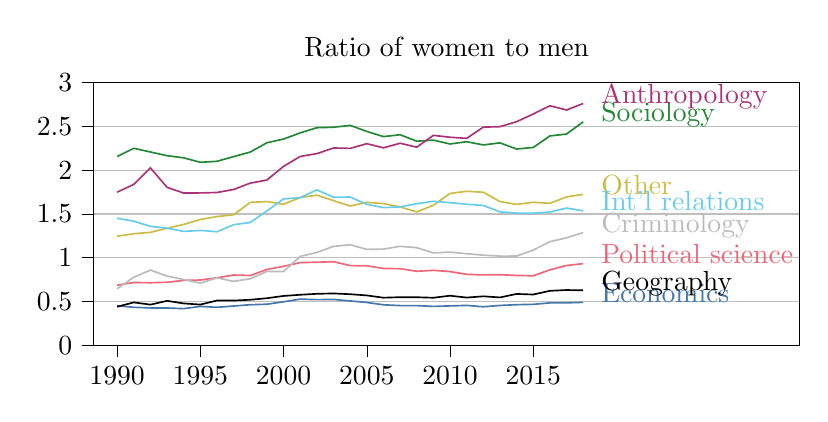
\begin{tikzpicture}

\definecolor{color0}{rgb}{0.266666666666667,0.466666666666667,0.666666666666667}
\definecolor{color1}{rgb}{0.933333333333333,0.4,0.466666666666667}
\definecolor{color2}{rgb}{0.133333333333333,0.533333333333333,0.2}
\definecolor{color3}{rgb}{0.8,0.733333333333333,0.266666666666667}
\definecolor{color4}{rgb}{0.4,0.8,0.933333333333333}
\definecolor{color5}{rgb}{0.666666666666667,0.2,0.466666666666667}

\begin{axis}[
height=140pt,
tick align=outside,
tick pos=left,
title={Ratio of women to men},
width=300pt,
x grid style={white!69.0196078431373!black},
xmin=1988.6, xmax=2031,
xtick style={color=black},
xtick={1990,1995,2000,2005,2010,2015},
xticklabels={\(\displaystyle 1990\),\(\displaystyle 1995\),\(\displaystyle 2000\),\(\displaystyle 2005\),\(\displaystyle 2010\),\(\displaystyle 2015\)},
ymajorgrids,
ymin=0, ymax=3,
ytick style={color=black},
ytick={0,0.5,1,1.5,2,2.5,3},
yticklabels={\(\displaystyle 0\),\(\displaystyle 0.5\),\(\displaystyle 1\),\(\displaystyle 1.5\),\(\displaystyle 2\),\(\displaystyle 2.5\),\(\displaystyle 3\)}
]
\addplot [semithick, color0]
table {%
1990 0.453454494476318
1991 0.434512615203857
1992 0.427694320678711
1993 0.426904916763306
1994 0.419453144073486
1995 0.444806575775146
1996 0.434596300125122
1998 0.464142203330994
1999 0.469876527786255
2000 0.497728705406189
2001 0.528073787689209
2002 0.521972298622131
2003 0.524367094039917
2005 0.490026116371155
2006 0.463130831718445
2007 0.454207539558411
2008 0.453919529914856
2009 0.445038676261902
2011 0.456213235855103
2012 0.440835237503052
2013 0.455652236938477
2014 0.464651584625244
2015 0.468673825263977
2016 0.484934091567993
2017 0.485498905181885
2018 0.491626977920532
};
\addplot [semithick, color1]
table {%
1990 0.687340497970581
1991 0.718239784240723
1992 0.715183019638062
1993 0.720339775085449
1994 0.741496920585632
1995 0.745949029922485
1996 0.771579146385193
1997 0.803107261657715
1998 0.797616720199585
1999 0.866689205169678
2000 0.902498960494995
2001 0.944846391677856
2002 0.949172735214233
2003 0.955212831497192
2004 0.910499453544617
2005 0.908062338829041
2006 0.878212213516235
2007 0.87516725063324
2008 0.845878720283508
2009 0.856622457504272
2010 0.84217095375061
2011 0.810709953308105
2012 0.804367065429688
2013 0.806700944900513
2014 0.798325777053833
2015 0.794228196144104
2016 0.862247109413147
2017 0.911926984786987
2018 0.932909369468689
};
\addplot [semithick, color2]
table {%
1990 2.15509796142578
1991 2.24903225898743
1993 2.16480875015259
1994 2.14018177986145
1995 2.08914875984192
1996 2.10084676742554
1997 2.15451312065125
1998 2.20654559135437
1999 2.31257438659668
2000 2.35462379455566
2001 2.42530727386475
2002 2.48414301872253
2003 2.48934626579285
2004 2.51065826416016
2005 2.44160652160645
2006 2.38261532783508
2007 2.40375828742981
2008 2.33004307746887
2009 2.34272146224976
2010 2.29821467399597
2011 2.32439589500427
2012 2.28757739067078
2013 2.31100392341614
2014 2.24083662033081
2015 2.25853753089905
2016 2.39009857177734
2017 2.41193509101868
2018 2.55055665969849
};
\addplot [semithick, color3]
table {%
1990 1.24622249603271
1991 1.27433001995087
1992 1.28972804546356
1993 1.33748888969421
1994 1.38074350357056
1995 1.43718707561493
1996 1.46975755691528
1997 1.49069452285767
1998 1.63201975822449
1999 1.6412159204483
2000 1.61032199859619
2001 1.68787050247192
2002 1.71428573131561
2004 1.5903924703598
2005 1.63254117965698
2006 1.61800968647003
2007 1.58040750026703
2008 1.52280271053314
2009 1.59942007064819
2010 1.7337794303894
2011 1.75879776477814
2012 1.74759149551392
2013 1.64136123657227
2014 1.60894978046417
2015 1.63310813903809
2016 1.62103271484375
2017 1.69435846805573
2018 1.7236739397049
};
\addplot [semithick, color4]
table {%
1990 1.45081532001495
1991 1.41702950000763
1992 1.35909819602966
1993 1.33774352073669
1994 1.30062794685364
1995 1.31255269050598
1996 1.29666662216187
1997 1.37724554538727
1998 1.40262174606323
1999 1.53457581996918
2000 1.67128205299377
2001 1.6860568523407
2002 1.77517664432526
2003 1.69076919555664
2004 1.69307291507721
2005 1.60994327068329
2006 1.57205748558044
2007 1.58068251609802
2008 1.61680722236633
2009 1.64477932453156
2010 1.62862813472748
2011 1.61050426959991
2012 1.59707045555115
2013 1.523766040802
2014 1.50999295711517
2015 1.5084331035614
2016 1.52219450473785
2017 1.56681549549103
2018 1.53559231758118
};
\addplot [semithick, color5]
table {%
1990 1.74866712093353
1991 1.83746552467346
1992 2.02597403526306
1993 1.80351257324219
1994 1.73820173740387
1995 1.7401157617569
1996 1.74474608898163
1997 1.77926981449127
1998 1.85183620452881
1999 1.8871773481369
2000 2.04300141334534
2001 2.15603137016296
2002 2.18847274780273
2003 2.25258803367615
2004 2.24808692932129
2005 2.30172061920166
2006 2.25455236434937
2007 2.30674362182617
2008 2.26183843612671
2009 2.39688038825989
2010 2.37516474723816
2011 2.36272668838501
2012 2.4907488822937
2013 2.49604296684265
2014 2.55269312858582
2015 2.64027833938599
2016 2.73464822769165
2017 2.68607902526855
2018 2.76014471054077
};
\addplot [semithick, white!73.3333333333333!black]
table {%
1990 0.646542310714722
1991 0.777292490005493
1992 0.859266519546509
1993 0.790786981582642
1994 0.75190258026123
1995 0.710562467575073
1996 0.770992279052734
1997 0.730769157409668
1998 0.760673522949219
1999 0.844403505325317
2000 0.842824578285217
2001 1.01557815074921
2002 1.06069529056549
2003 1.1302604675293
2004 1.14858710765839
2005 1.09585392475128
2006 1.09888970851898
2007 1.13046622276306
2008 1.11553645133972
2009 1.05514574050903
2010 1.06476509571075
2011 1.04630792140961
2012 1.02961671352386
2013 1.01904761791229
2014 1.01933991909027
2015 1.08761656284332
2016 1.18314814567566
2017 1.22725999355316
2018 1.28747606277466
};
\addplot [semithick, black]
table {%
1990 0.441163301467896
1991 0.490615487098694
1992 0.46512508392334
1993 0.508511424064636
1994 0.478793859481812
1995 0.465986371040344
1996 0.512168526649475
1997 0.511687278747559
1998 0.520879149436951
1999 0.538490056991577
2000 0.564280271530151
2001 0.577753305435181
2002 0.588586330413818
2003 0.592862367630005
2004 0.584151744842529
2005 0.570275783538818
2006 0.544358968734741
2007 0.550142288208008
2008 0.549592018127441
2009 0.543748140335083
2010 0.567093133926392
2011 0.545867681503296
2012 0.560144186019897
2013 0.5474613904953
2014 0.587161302566528
2015 0.580625534057617
2016 0.622629404067993
2017 0.63182270526886
2018 0.628732562065125
};
\draw (axis cs:2018.5,0.491626926915826) node[
  anchor=base west,
  text=color0,
  rotate=0.0
]{Economics};
\draw (axis cs:2018.5,0.932909364532259) node[
  anchor=base west,
  text=color1,
  rotate=0.0
]{Political science};
\draw (axis cs:2018.5,2.55055658627087) node[
  anchor=base west,
  text=color2,
  rotate=0.0
]{Sociology};
\draw (axis cs:2018.5,1.72367399741268) node[
  anchor=base west,
  text=color3,
  rotate=0.0
]{Other};
\draw (axis cs:2018.5,1.53559232991857) node[
  anchor=base west,
  text=color4,
  rotate=0.0
]{Int'l relations};
\draw (axis cs:2018.5,2.76014463640016) node[
  anchor=base west,
  text=color5,
  rotate=0.0
]{Anthropology};
\draw (axis cs:2018.5,1.28747602082762) node[
  anchor=base west,
  text=white!73.3333333333333!black,
  rotate=0.0
]{Criminology};
\draw (axis cs:2018.5,0.628732581287326) node[
  anchor=base west,
  text=black,
  rotate=0.0
]{Geography};
\end{axis}

\end{tikzpicture}

\vspace{0.1cm}
\begin{tikzpicture}
% This file was created by tikzplotlib v0.9.2.
\definecolor{color0}{rgb}{0.266666666666667,0.466666666666667,0.666666666666667}
\definecolor{color1}{rgb}{0.933333333333333,0.4,0.466666666666667}
\definecolor{color2}{rgb}{0.133333333333333,0.533333333333333,0.2}
\definecolor{color3}{rgb}{0.8,0.733333333333333,0.266666666666667}
\definecolor{color4}{rgb}{0.4,0.8,0.933333333333333}
\definecolor{color5}{rgb}{0.666666666666667,0.2,0.466666666666667}

\begin{groupplot}[group style={group size=2 by 1, group name=my plots, horizontal sep=0.8cm}]
\nextgroupplot[
height=90pt, width=160pt,
legend style={at={(2.02, 0.5)},anchor=west,},
reverse legend,
tick align=outside,
tick pos=left,
x grid style={white!69.0196078431373!black},
xlabel={Women},
xmin=1988.6, xmax=2019.4,
xtick style={color=black},
xtick={1990,2000,2010},
xticklabels={\(\displaystyle 1990\),\(\displaystyle 2000\),\(\displaystyle 2010\)},
ymajorgrids,
ymin=0, ymax=87.6897,
ytick style={color=black}
]
\path [draw=color0, fill=color0]
(axis cs:1990,7.482)
--(axis cs:1990,0)
--(axis cs:1991,0)
--(axis cs:1992,0)
--(axis cs:1993,0)
--(axis cs:1994,0)
--(axis cs:1995,0)
--(axis cs:1996,0)
--(axis cs:1997,0)
--(axis cs:1998,0)
--(axis cs:1999,0)
--(axis cs:2000,0)
--(axis cs:2001,0)
--(axis cs:2002,0)
--(axis cs:2003,0)
--(axis cs:2004,0)
--(axis cs:2005,0)
--(axis cs:2006,0)
--(axis cs:2007,0)
--(axis cs:2008,0)
--(axis cs:2009,0)
--(axis cs:2010,0)
--(axis cs:2011,0)
--(axis cs:2012,0)
--(axis cs:2013,0)
--(axis cs:2014,0)
--(axis cs:2015,0)
--(axis cs:2016,0)
--(axis cs:2017,0)
--(axis cs:2018,0)
--(axis cs:2018,13.299)
--(axis cs:2018,13.299)
--(axis cs:2017,12.756)
--(axis cs:2016,12.521)
--(axis cs:2015,11.924)
--(axis cs:2014,10.93)
--(axis cs:2013,10.218)
--(axis cs:2012,9.88)
--(axis cs:2011,10.221)
--(axis cs:2010,9.718)
--(axis cs:2009,9.154)
--(axis cs:2008,8.9)
--(axis cs:2007,8.431)
--(axis cs:2006,8.479)
--(axis cs:2005,8.991)
--(axis cs:2004,9.083)
--(axis cs:2003,8.823)
--(axis cs:2002,7.982)
--(axis cs:2001,7.383)
--(axis cs:2000,6.136)
--(axis cs:1999,5.631)
--(axis cs:1998,5.43)
--(axis cs:1997,5.153)
--(axis cs:1996,5.07)
--(axis cs:1995,5.46)
--(axis cs:1994,5.783)
--(axis cs:1993,6.404)
--(axis cs:1992,7.036)
--(axis cs:1991,7.136)
--(axis cs:1990,7.482)
--cycle;

\path [draw=color1, fill=color1]
(axis cs:1990,21.224)
--(axis cs:1990,7.482)
--(axis cs:1991,7.136)
--(axis cs:1992,7.036)
--(axis cs:1993,6.404)
--(axis cs:1994,5.783)
--(axis cs:1995,5.46)
--(axis cs:1996,5.07)
--(axis cs:1997,5.153)
--(axis cs:1998,5.43)
--(axis cs:1999,5.631)
--(axis cs:2000,6.136)
--(axis cs:2001,7.383)
--(axis cs:2002,7.982)
--(axis cs:2003,8.823)
--(axis cs:2004,9.083)
--(axis cs:2005,8.991)
--(axis cs:2006,8.479)
--(axis cs:2007,8.431)
--(axis cs:2008,8.9)
--(axis cs:2009,9.154)
--(axis cs:2010,9.718)
--(axis cs:2011,10.221)
--(axis cs:2012,9.88)
--(axis cs:2013,10.218)
--(axis cs:2014,10.93)
--(axis cs:2015,11.924)
--(axis cs:2016,12.521)
--(axis cs:2017,12.756)
--(axis cs:2018,13.299)
--(axis cs:2018,32.516)
--(axis cs:2018,32.516)
--(axis cs:2017,31.259)
--(axis cs:2016,30.379)
--(axis cs:2015,29.675)
--(axis cs:2014,29.622)
--(axis cs:2013,29.528)
--(axis cs:2012,29.846)
--(axis cs:2011,30.432)
--(axis cs:2010,29.952)
--(axis cs:2009,29.378)
--(axis cs:2008,29.476)
--(axis cs:2007,29.365)
--(axis cs:2006,29.189)
--(axis cs:2005,29.377)
--(axis cs:2004,28.005)
--(axis cs:2003,26.781)
--(axis cs:2002,23.874)
--(axis cs:2001,22.27)
--(axis cs:2000,19.354)
--(axis cs:1999,18.471)
--(axis cs:1998,17.947)
--(axis cs:1997,18.128)
--(axis cs:1996,18.541)
--(axis cs:1995,19.639)
--(axis cs:1994,21.218)
--(axis cs:1993,22.348)
--(axis cs:1992,22.863)
--(axis cs:1991,22.135)
--(axis cs:1990,21.224)
--cycle;

\path [draw=color2, fill=color2]
(axis cs:1990,32.215)
--(axis cs:1990,21.224)
--(axis cs:1991,22.135)
--(axis cs:1992,22.863)
--(axis cs:1993,22.348)
--(axis cs:1994,21.218)
--(axis cs:1995,19.639)
--(axis cs:1996,18.541)
--(axis cs:1997,18.128)
--(axis cs:1998,17.947)
--(axis cs:1999,18.471)
--(axis cs:2000,19.354)
--(axis cs:2001,22.27)
--(axis cs:2002,23.874)
--(axis cs:2003,26.781)
--(axis cs:2004,28.005)
--(axis cs:2005,29.377)
--(axis cs:2006,29.189)
--(axis cs:2007,29.365)
--(axis cs:2008,29.476)
--(axis cs:2009,29.378)
--(axis cs:2010,29.952)
--(axis cs:2011,30.432)
--(axis cs:2012,29.846)
--(axis cs:2013,29.528)
--(axis cs:2014,29.622)
--(axis cs:2015,29.675)
--(axis cs:2016,30.379)
--(axis cs:2017,31.259)
--(axis cs:2018,32.516)
--(axis cs:2018,54.512)
--(axis cs:2018,54.512)
--(axis cs:2017,52.923)
--(axis cs:2016,52.442)
--(axis cs:2015,52.161)
--(axis cs:2014,52.976)
--(axis cs:2013,53.47)
--(axis cs:2012,53.527)
--(axis cs:2011,53.232)
--(axis cs:2010,52.093)
--(axis cs:2009,51.587)
--(axis cs:2008,51.665)
--(axis cs:2007,52.006)
--(axis cs:2006,51.364)
--(axis cs:2005,51.747)
--(axis cs:2004,49.323)
--(axis cs:2003,47.226)
--(axis cs:2002,43.613)
--(axis cs:2001,41.801)
--(axis cs:2000,37.381)
--(axis cs:1999,35.961)
--(axis cs:1998,35.072)
--(axis cs:1997,35.028)
--(axis cs:1996,34.915)
--(axis cs:1995,35.176)
--(axis cs:1994,36.531)
--(axis cs:1993,36.718)
--(axis cs:1992,36.384)
--(axis cs:1991,34.336)
--(axis cs:1990,32.215)
--cycle;

\path [draw=color3, fill=color3]
(axis cs:1990,37.246)
--(axis cs:1990,32.215)
--(axis cs:1991,34.336)
--(axis cs:1992,36.384)
--(axis cs:1993,36.718)
--(axis cs:1994,36.531)
--(axis cs:1995,35.176)
--(axis cs:1996,34.915)
--(axis cs:1997,35.028)
--(axis cs:1998,35.072)
--(axis cs:1999,35.961)
--(axis cs:2000,37.381)
--(axis cs:2001,41.801)
--(axis cs:2002,43.613)
--(axis cs:2003,47.226)
--(axis cs:2004,49.323)
--(axis cs:2005,51.747)
--(axis cs:2006,51.364)
--(axis cs:2007,52.006)
--(axis cs:2008,51.665)
--(axis cs:2009,51.587)
--(axis cs:2010,52.093)
--(axis cs:2011,53.232)
--(axis cs:2012,53.527)
--(axis cs:2013,53.47)
--(axis cs:2014,52.976)
--(axis cs:2015,52.161)
--(axis cs:2016,52.442)
--(axis cs:2017,52.923)
--(axis cs:2018,54.512)
--(axis cs:2018,61.174)
--(axis cs:2018,61.174)
--(axis cs:2017,60.041)
--(axis cs:2016,59.286)
--(axis cs:2015,59.412)
--(axis cs:2014,60.958)
--(axis cs:2013,62.248)
--(axis cs:2012,62.597)
--(axis cs:2011,62.478)
--(axis cs:2010,60.644)
--(axis cs:2009,59.309)
--(axis cs:2008,59.011)
--(axis cs:2007,59.298)
--(axis cs:2006,58.713)
--(axis cs:2005,58.891)
--(axis cs:2004,56.739)
--(axis cs:2003,54.845)
--(axis cs:2002,51.437)
--(axis cs:2001,49.204)
--(axis cs:2000,44.183)
--(axis cs:1999,42.818)
--(axis cs:1998,41.698)
--(axis cs:1997,41.596)
--(axis cs:1996,41.16)
--(axis cs:1995,41.205)
--(axis cs:1994,42.511)
--(axis cs:1993,42.726)
--(axis cs:1992,42.122)
--(axis cs:1991,39.757)
--(axis cs:1990,37.246)
--cycle;

\path [draw=color4, fill=color4]
(axis cs:1990,40.004)
--(axis cs:1990,37.246)
--(axis cs:1991,39.757)
--(axis cs:1992,42.122)
--(axis cs:1993,42.726)
--(axis cs:1994,42.511)
--(axis cs:1995,41.205)
--(axis cs:1996,41.16)
--(axis cs:1997,41.596)
--(axis cs:1998,41.698)
--(axis cs:1999,42.818)
--(axis cs:2000,44.183)
--(axis cs:2001,49.204)
--(axis cs:2002,51.437)
--(axis cs:2003,54.845)
--(axis cs:2004,56.739)
--(axis cs:2005,58.891)
--(axis cs:2006,58.713)
--(axis cs:2007,59.298)
--(axis cs:2008,59.011)
--(axis cs:2009,59.309)
--(axis cs:2010,60.644)
--(axis cs:2011,62.478)
--(axis cs:2012,62.597)
--(axis cs:2013,62.248)
--(axis cs:2014,60.958)
--(axis cs:2015,59.412)
--(axis cs:2016,59.286)
--(axis cs:2017,60.041)
--(axis cs:2018,61.174)
--(axis cs:2018,67.02)
--(axis cs:2018,67.02)
--(axis cs:2017,66.009)
--(axis cs:2016,65.39)
--(axis cs:2015,65.583)
--(axis cs:2014,67.38)
--(axis cs:2013,68.916)
--(axis cs:2012,69.466)
--(axis cs:2011,69.408)
--(axis cs:2010,67.209)
--(axis cs:2009,65.421)
--(axis cs:2008,64.956)
--(axis cs:2007,64.764)
--(axis cs:2006,64.069)
--(axis cs:2005,63.716)
--(axis cs:2004,61.334)
--(axis cs:2003,59.241)
--(axis cs:2002,55.456)
--(axis cs:2001,53.001)
--(axis cs:2000,47.442)
--(axis cs:1999,45.947)
--(axis cs:1998,44.694)
--(axis cs:1997,44.586)
--(axis cs:1996,44.272)
--(axis cs:1995,44.321)
--(axis cs:1994,45.825)
--(axis cs:1993,46.366)
--(axis cs:1992,45.498)
--(axis cs:1991,42.686)
--(axis cs:1990,40.004)
--cycle;

\path [draw=color5, fill=color5]
(axis cs:1990,42.3)
--(axis cs:1990,40.004)
--(axis cs:1991,42.686)
--(axis cs:1992,45.498)
--(axis cs:1993,46.366)
--(axis cs:1994,45.825)
--(axis cs:1995,44.321)
--(axis cs:1996,44.272)
--(axis cs:1997,44.586)
--(axis cs:1998,44.694)
--(axis cs:1999,45.947)
--(axis cs:2000,47.442)
--(axis cs:2001,53.001)
--(axis cs:2002,55.456)
--(axis cs:2003,59.241)
--(axis cs:2004,61.334)
--(axis cs:2005,63.716)
--(axis cs:2006,64.069)
--(axis cs:2007,64.764)
--(axis cs:2008,64.956)
--(axis cs:2009,65.421)
--(axis cs:2010,67.209)
--(axis cs:2011,69.408)
--(axis cs:2012,69.466)
--(axis cs:2013,68.916)
--(axis cs:2014,67.38)
--(axis cs:2015,65.583)
--(axis cs:2016,65.39)
--(axis cs:2017,66.009)
--(axis cs:2018,67.02)
--(axis cs:2018,73.89)
--(axis cs:2018,73.89)
--(axis cs:2017,72.743)
--(axis cs:2016,72.738)
--(axis cs:2015,73.554)
--(axis cs:2014,76.1)
--(axis cs:2013,77.747)
--(axis cs:2012,77.947)
--(axis cs:2011,76.964)
--(axis cs:2010,74.42)
--(axis cs:2009,72.336)
--(axis cs:2008,71.452)
--(axis cs:2007,70.75)
--(axis cs:2006,70.012)
--(axis cs:2005,69.468)
--(axis cs:2004,66.916)
--(axis cs:2003,64.681)
--(axis cs:2002,60.658)
--(axis cs:2001,57.934)
--(axis cs:2000,52.098)
--(axis cs:1999,50.48)
--(axis cs:1998,49.081)
--(axis cs:1997,48.826)
--(axis cs:1996,48.257)
--(axis cs:1995,47.93)
--(axis cs:1994,49.324)
--(axis cs:1993,49.652)
--(axis cs:1992,48.618)
--(axis cs:1991,45.354)
--(axis cs:1990,42.3)
--cycle;

\path [draw=white!73.3333333333333!black, fill=white!73.3333333333333!black]
(axis cs:1990,42.889)
--(axis cs:1990,42.3)
--(axis cs:1991,45.354)
--(axis cs:1992,48.618)
--(axis cs:1993,49.652)
--(axis cs:1994,49.324)
--(axis cs:1995,47.93)
--(axis cs:1996,48.257)
--(axis cs:1997,48.826)
--(axis cs:1998,49.081)
--(axis cs:1999,50.48)
--(axis cs:2000,52.098)
--(axis cs:2001,57.934)
--(axis cs:2002,60.658)
--(axis cs:2003,64.681)
--(axis cs:2004,66.916)
--(axis cs:2005,69.468)
--(axis cs:2006,70.012)
--(axis cs:2007,70.75)
--(axis cs:2008,71.452)
--(axis cs:2009,72.336)
--(axis cs:2010,74.42)
--(axis cs:2011,76.964)
--(axis cs:2012,77.947)
--(axis cs:2013,77.747)
--(axis cs:2014,76.1)
--(axis cs:2015,73.554)
--(axis cs:2016,72.738)
--(axis cs:2017,72.743)
--(axis cs:2018,73.89)
--(axis cs:2018,78.588)
--(axis cs:2018,78.588)
--(axis cs:2017,77.128)
--(axis cs:2016,77.105)
--(axis cs:2015,77.638)
--(axis cs:2014,80.053)
--(axis cs:2013,81.492)
--(axis cs:2012,81.493)
--(axis cs:2011,80.308)
--(axis cs:2010,77.593)
--(axis cs:2009,75.34)
--(axis cs:2008,74.561)
--(axis cs:2007,73.878)
--(axis cs:2006,73.179)
--(axis cs:2005,72.349)
--(axis cs:2004,69.436)
--(axis cs:2003,66.937)
--(axis cs:2002,62.458)
--(axis cs:2001,59.629)
--(axis cs:2000,53.578)
--(axis cs:1999,51.853)
--(axis cs:1998,50.346)
--(axis cs:1997,50.042)
--(axis cs:1996,49.469)
--(axis cs:1995,48.966)
--(axis cs:1994,50.312)
--(axis cs:1993,50.476)
--(axis cs:1992,49.485)
--(axis cs:1991,46.066)
--(axis cs:1990,42.889)
--cycle;

\path [draw=black, fill=black]
(axis cs:1990,43.875)
--(axis cs:1990,42.889)
--(axis cs:1991,46.066)
--(axis cs:1992,49.485)
--(axis cs:1993,50.476)
--(axis cs:1994,50.312)
--(axis cs:1995,48.966)
--(axis cs:1996,49.469)
--(axis cs:1997,50.042)
--(axis cs:1998,50.346)
--(axis cs:1999,51.853)
--(axis cs:2000,53.578)
--(axis cs:2001,59.629)
--(axis cs:2002,62.458)
--(axis cs:2003,66.937)
--(axis cs:2004,69.436)
--(axis cs:2005,72.349)
--(axis cs:2006,73.179)
--(axis cs:2007,73.878)
--(axis cs:2008,74.561)
--(axis cs:2009,75.34)
--(axis cs:2010,77.593)
--(axis cs:2011,80.308)
--(axis cs:2012,81.493)
--(axis cs:2013,81.492)
--(axis cs:2014,80.053)
--(axis cs:2015,77.638)
--(axis cs:2016,77.105)
--(axis cs:2017,77.128)
--(axis cs:2018,78.588)
--(axis cs:2018,80.483)
--(axis cs:2018,80.483)
--(axis cs:2017,79.038)
--(axis cs:2016,79.042)
--(axis cs:2015,79.55)
--(axis cs:2014,82.047)
--(axis cs:2013,83.476)
--(axis cs:2012,83.514)
--(axis cs:2011,82.23)
--(axis cs:2010,79.499)
--(axis cs:2009,77.136)
--(axis cs:2008,76.312)
--(axis cs:2007,75.617)
--(axis cs:2006,74.805)
--(axis cs:2005,74.045)
--(axis cs:2004,71.161)
--(axis cs:2003,68.565)
--(axis cs:2002,64.036)
--(axis cs:2001,61.208)
--(axis cs:2000,55.044)
--(axis cs:1999,53.301)
--(axis cs:1998,51.768)
--(axis cs:1997,51.443)
--(axis cs:1996,50.879)
--(axis cs:1995,50.336)
--(axis cs:1994,51.757)
--(axis cs:1993,51.88)
--(axis cs:1992,50.712)
--(axis cs:1991,47.19)
--(axis cs:1990,43.875)
--cycle;

\addplot [semithick, color0]
table {%
1990 7.48199987411499
1991 7.13600015640259
1992 7.03599977493286
1993 6.40399980545044
1994 5.78299999237061
1995 5.46000003814697
1996 5.07000017166138
1997 5.15299987792969
1998 5.42999982833862
1999 5.63100004196167
2000 6.13600015640259
2001 7.38299989700317
2002 7.98199987411499
2003 8.82299995422363
2004 9.08300018310547
2005 8.99100017547607
2006 8.47900009155273
2007 8.43099975585938
2008 8.89999961853027
2009 9.1540002822876
2010 9.7180004119873
2011 10.2209997177124
2012 9.88000011444092
2013 10.2180004119873
2014 10.9300003051758
2015 11.923999786377
2016 12.5209999084473
2017 12.7559995651245
2018 13.298999786377
};
\addplot [semithick, color1]
table {%
1990 21.2240009307861
1991 22.1350002288818
1992 22.863000869751
1993 22.3479995727539
1994 21.2180004119873
1995 19.6389999389648
1996 18.5410003662109
1997 18.1280002593994
1998 17.94700050354
1999 18.4710006713867
2000 19.3540000915527
2001 22.2700004577637
2002 23.8740005493164
2003 26.7810001373291
2004 28.0049991607666
2005 29.3770008087158
2006 29.1889991760254
2007 29.3649997711182
2008 29.4759998321533
2009 29.3780002593994
2010 29.9519996643066
2011 30.431999206543
2012 29.8460006713867
2013 29.5279998779297
2014 29.6219997406006
2015 29.6749992370605
2016 30.378999710083
2017 31.2590007781982
2018 32.515998840332
};
\addplot [semithick, color2]
table {%
1990 32.2150001525879
1991 34.3359985351562
1992 36.3839988708496
1993 36.7179985046387
1994 36.5309982299805
1995 35.1759986877441
1996 34.9150009155273
1997 35.0279998779297
1998 35.0719985961914
1999 35.9609985351562
2000 37.3810005187988
2001 41.8009986877441
2002 43.6129989624023
2003 47.226001739502
2004 49.3230018615723
2005 51.7470016479492
2006 51.3639984130859
2007 52.0060005187988
2008 51.6650009155273
2009 51.5870018005371
2010 52.0929985046387
2011 53.2319984436035
2012 53.5270004272461
2013 53.4700012207031
2014 52.976001739502
2015 52.1609992980957
2016 52.4420013427734
2017 52.9230003356934
2018 54.5120010375977
};
\addplot [semithick, color3]
table {%
1990 37.2459983825684
1991 39.7569999694824
1992 42.1220016479492
1993 42.726001739502
1994 42.5110015869141
1995 41.2050018310547
1996 41.1599998474121
1997 41.5960006713867
1998 41.6980018615723
1999 42.818000793457
2000 44.1829986572266
2001 49.2039985656738
2002 51.4370002746582
2003 54.8450012207031
2004 56.7389984130859
2005 58.890998840332
2006 58.7130012512207
2007 59.2980003356934
2008 59.0110015869141
2009 59.3089981079102
2010 60.6440010070801
2011 62.4780006408691
2012 62.5970001220703
2013 62.2480010986328
2014 60.9580001831055
2015 59.4119987487793
2016 59.2859992980957
2017 60.0410003662109
2018 61.173999786377
};
\addplot [semithick, color4]
table {%
1990 40.0040016174316
1991 42.6860008239746
1992 45.4980010986328
1993 46.3660011291504
1994 45.8250007629395
1995 44.3209991455078
1996 44.2719993591309
1997 44.5859985351562
1998 44.6940002441406
1999 45.9469985961914
2000 47.4420013427734
2001 53.0009994506836
2002 55.4560012817383
2003 59.2410011291504
2004 61.3339996337891
2005 63.7159996032715
2006 64.0690002441406
2007 64.7639999389648
2008 64.9560012817383
2009 65.4209976196289
2010 67.2089996337891
2011 69.4079971313477
2012 69.4660034179688
2013 68.9160003662109
2014 67.379997253418
2015 65.5830001831055
2016 65.3899993896484
2017 66.0090026855469
2018 67.0199966430664
};
\addplot [semithick, color5]
table {%
1990 42.2999992370605
1991 45.3540000915527
1992 48.6180000305176
1993 49.6520004272461
1994 49.3240013122559
1995 47.9300003051758
1996 48.2569999694824
1997 48.826000213623
1998 49.0810012817383
1999 50.4799995422363
2000 52.0979995727539
2001 57.9339981079102
2002 60.6580009460449
2003 64.6809997558594
2004 66.9160003662109
2005 69.4680023193359
2006 70.0120010375977
2007 70.75
2008 71.4520034790039
2009 72.3359985351562
2010 74.4199981689453
2011 76.963996887207
2012 77.9469985961914
2013 77.7470016479492
2014 76.0999984741211
2015 73.5540008544922
2016 72.7379989624023
2017 72.7429962158203
2018 73.8899993896484
};
\addplot [semithick, white!73.3333333333333!black]
table {%
1990 42.8889999389648
1991 46.0660018920898
1992 49.4850006103516
1993 50.476001739502
1994 50.3120002746582
1995 48.9659996032715
1996 49.4690017700195
1997 50.0419998168945
1998 50.3460006713867
1999 51.8530006408691
2000 53.5779991149902
2001 59.6290016174316
2002 62.4580001831055
2003 66.9369964599609
2004 69.4359970092773
2005 72.3489990234375
2006 73.1790008544922
2007 73.8779983520508
2008 74.5609970092773
2009 75.3399963378906
2010 77.5930023193359
2011 80.3079986572266
2012 81.4929962158203
2013 81.4919967651367
2014 80.0530014038086
2015 77.6380004882812
2016 77.1050033569336
2017 77.1279983520508
2018 78.5879974365234
};
\addplot [semithick, black]
table {%
1990 43.875
1991 47.189998626709
1992 50.7120018005371
1993 51.8800010681152
1994 51.7569999694824
1995 50.3359985351562
1996 50.8790016174316
1997 51.443000793457
1998 51.7680015563965
1999 53.3009986877441
2000 55.0439987182617
2001 61.2080001831055
2002 64.036003112793
2003 68.5650024414062
2004 71.161003112793
2005 74.0449981689453
2006 74.8050003051758
2007 75.6169967651367
2008 76.3119964599609
2009 77.1360015869141
2010 79.4990005493164
2011 82.2300033569336
2012 83.5139999389648
2013 83.4759979248047
2014 82.0469970703125
2015 79.5500030517578
2016 79.0419998168945
2017 79.0380020141602
2018 80.4830017089844
};

\nextgroupplot[
height=90pt, width=160pt,
legend style={at={(2.02, 0.5)},anchor=west,},
reverse legend,
scaled y ticks=manual:{}{\pgfmathparse{#1}},
tick align=outside,
tick pos=left,
x grid style={white!69.0196078431373!black},
xlabel={Men},
xmin=1988.6, xmax=2019.4,
xtick style={color=black},
xtick={1990,2000,2010},
xticklabels={\(\displaystyle 1990\),\(\displaystyle 2000\),\(\displaystyle 2010\)},
ymajorgrids,
ymin=0, ymax=87.6897,
ytick style={color=black},
yticklabels={}
]
\path [draw=color0, fill=color0]
(axis cs:1990,16.5)
--(axis cs:1990,0)
--(axis cs:1991,0)
--(axis cs:1992,0)
--(axis cs:1993,0)
--(axis cs:1994,0)
--(axis cs:1995,0)
--(axis cs:1996,0)
--(axis cs:1997,0)
--(axis cs:1998,0)
--(axis cs:1999,0)
--(axis cs:2000,0)
--(axis cs:2001,0)
--(axis cs:2002,0)
--(axis cs:2003,0)
--(axis cs:2004,0)
--(axis cs:2005,0)
--(axis cs:2006,0)
--(axis cs:2007,0)
--(axis cs:2008,0)
--(axis cs:2009,0)
--(axis cs:2010,0)
--(axis cs:2011,0)
--(axis cs:2012,0)
--(axis cs:2013,0)
--(axis cs:2014,0)
--(axis cs:2015,0)
--(axis cs:2016,0)
--(axis cs:2017,0)
--(axis cs:2018,0)
--(axis cs:2018,27.051)
--(axis cs:2018,27.051)
--(axis cs:2017,26.274)
--(axis cs:2016,25.82)
--(axis cs:2015,25.442)
--(axis cs:2014,23.523)
--(axis cs:2013,22.425)
--(axis cs:2012,22.412)
--(axis cs:2011,22.404)
--(axis cs:2010,21.547)
--(axis cs:2009,20.569)
--(axis cs:2008,19.607)
--(axis cs:2007,18.562)
--(axis cs:2006,18.308)
--(axis cs:2005,18.348)
--(axis cs:2004,17.899)
--(axis cs:2003,16.826)
--(axis cs:2002,15.292)
--(axis cs:2001,13.981)
--(axis cs:2000,12.328)
--(axis cs:1999,11.984)
--(axis cs:1998,11.699)
--(axis cs:1997,11.473)
--(axis cs:1996,11.666)
--(axis cs:1995,12.275)
--(axis cs:1994,13.787)
--(axis cs:1993,15.001)
--(axis cs:1992,16.451)
--(axis cs:1991,16.423)
--(axis cs:1990,16.5)
--cycle;

\path [draw=color1, fill=color1]
(axis cs:1990,36.493)
--(axis cs:1990,16.5)
--(axis cs:1991,16.423)
--(axis cs:1992,16.451)
--(axis cs:1993,15.001)
--(axis cs:1994,13.787)
--(axis cs:1995,12.275)
--(axis cs:1996,11.666)
--(axis cs:1997,11.473)
--(axis cs:1998,11.699)
--(axis cs:1999,11.984)
--(axis cs:2000,12.328)
--(axis cs:2001,13.981)
--(axis cs:2002,15.292)
--(axis cs:2003,16.826)
--(axis cs:2004,17.899)
--(axis cs:2005,18.348)
--(axis cs:2006,18.308)
--(axis cs:2007,18.562)
--(axis cs:2008,19.607)
--(axis cs:2009,20.569)
--(axis cs:2010,21.547)
--(axis cs:2011,22.404)
--(axis cs:2012,22.412)
--(axis cs:2013,22.425)
--(axis cs:2014,23.523)
--(axis cs:2015,25.442)
--(axis cs:2016,25.82)
--(axis cs:2017,26.274)
--(axis cs:2018,27.051)
--(axis cs:2018,47.65)
--(axis cs:2018,47.65)
--(axis cs:2017,46.564)
--(axis cs:2016,46.531)
--(axis cs:2015,47.792)
--(axis cs:2014,46.937)
--(axis cs:2013,46.362)
--(axis cs:2012,47.234)
--(axis cs:2011,47.334)
--(axis cs:2010,45.573)
--(axis cs:2009,44.178)
--(axis cs:2008,43.932)
--(axis cs:2007,42.482)
--(axis cs:2006,41.89)
--(axis cs:2005,40.798)
--(axis cs:2004,38.681)
--(axis cs:2003,35.626)
--(axis cs:2002,32.035)
--(axis cs:2001,29.737)
--(axis cs:2000,26.974)
--(axis cs:1999,26.799)
--(axis cs:1998,27.392)
--(axis cs:1997,27.629)
--(axis cs:1996,29.125)
--(axis cs:1995,31.283)
--(axis cs:1994,34.603)
--(axis cs:1993,37.135)
--(axis cs:1992,38.581)
--(axis cs:1991,37.306)
--(axis cs:1990,36.493)
--cycle;

\path [draw=color2, fill=color2]
(axis cs:1990,41.593)
--(axis cs:1990,36.493)
--(axis cs:1991,37.306)
--(axis cs:1992,38.581)
--(axis cs:1993,37.135)
--(axis cs:1994,34.603)
--(axis cs:1995,31.283)
--(axis cs:1996,29.125)
--(axis cs:1997,27.629)
--(axis cs:1998,27.392)
--(axis cs:1999,26.799)
--(axis cs:2000,26.974)
--(axis cs:2001,29.737)
--(axis cs:2002,32.035)
--(axis cs:2003,35.626)
--(axis cs:2004,38.681)
--(axis cs:2005,40.798)
--(axis cs:2006,41.89)
--(axis cs:2007,42.482)
--(axis cs:2008,43.932)
--(axis cs:2009,44.178)
--(axis cs:2010,45.573)
--(axis cs:2011,47.334)
--(axis cs:2012,47.234)
--(axis cs:2013,46.362)
--(axis cs:2014,46.937)
--(axis cs:2015,47.792)
--(axis cs:2016,46.531)
--(axis cs:2017,46.564)
--(axis cs:2018,47.65)
--(axis cs:2018,56.274)
--(axis cs:2018,56.274)
--(axis cs:2017,55.546)
--(axis cs:2016,55.762)
--(axis cs:2015,57.748)
--(axis cs:2014,57.359)
--(axis cs:2013,56.722)
--(axis cs:2012,57.586)
--(axis cs:2011,57.143)
--(axis cs:2010,55.207)
--(axis cs:2009,53.658)
--(axis cs:2008,53.455)
--(axis cs:2007,51.901)
--(axis cs:2006,51.197)
--(axis cs:2005,49.96)
--(axis cs:2004,47.172)
--(axis cs:2003,43.839)
--(axis cs:2002,39.981)
--(axis cs:2001,37.79)
--(axis cs:2000,34.63)
--(axis cs:1999,34.362)
--(axis cs:1998,35.153)
--(axis cs:1997,35.473)
--(axis cs:1996,36.919)
--(axis cs:1995,38.72)
--(axis cs:1994,41.758)
--(axis cs:1993,43.773)
--(axis cs:1992,44.708)
--(axis cs:1991,42.731)
--(axis cs:1990,41.593)
--cycle;

\path [draw=color3, fill=color3]
(axis cs:1990,45.63)
--(axis cs:1990,41.593)
--(axis cs:1991,42.731)
--(axis cs:1992,44.708)
--(axis cs:1993,43.773)
--(axis cs:1994,41.758)
--(axis cs:1995,38.72)
--(axis cs:1996,36.919)
--(axis cs:1997,35.473)
--(axis cs:1998,35.153)
--(axis cs:1999,34.362)
--(axis cs:2000,34.63)
--(axis cs:2001,37.79)
--(axis cs:2002,39.981)
--(axis cs:2003,43.839)
--(axis cs:2004,47.172)
--(axis cs:2005,49.96)
--(axis cs:2006,51.197)
--(axis cs:2007,51.901)
--(axis cs:2008,53.455)
--(axis cs:2009,53.658)
--(axis cs:2010,55.207)
--(axis cs:2011,57.143)
--(axis cs:2012,57.586)
--(axis cs:2013,56.722)
--(axis cs:2014,57.359)
--(axis cs:2015,57.748)
--(axis cs:2016,55.762)
--(axis cs:2017,55.546)
--(axis cs:2018,56.274)
--(axis cs:2018,60.139)
--(axis cs:2018,60.139)
--(axis cs:2017,59.747)
--(axis cs:2016,59.984)
--(axis cs:2015,62.188)
--(axis cs:2014,62.32)
--(axis cs:2013,62.07)
--(axis cs:2012,62.776)
--(axis cs:2011,62.4)
--(axis cs:2010,60.139)
--(axis cs:2009,58.486)
--(axis cs:2008,58.279)
--(axis cs:2007,56.515)
--(axis cs:2006,55.739)
--(axis cs:2005,54.336)
--(axis cs:2004,51.835)
--(axis cs:2003,48.45)
--(axis cs:2002,44.545)
--(axis cs:2001,42.176)
--(axis cs:2000,38.854)
--(axis cs:1999,38.54)
--(axis cs:1998,39.213)
--(axis cs:1997,39.879)
--(axis cs:1996,41.168)
--(axis cs:1995,42.915)
--(axis cs:1994,46.089)
--(axis cs:1993,48.265)
--(axis cs:1992,49.157)
--(axis cs:1991,46.985)
--(axis cs:1990,45.63)
--cycle;

\path [draw=color4, fill=color4]
(axis cs:1990,47.531)
--(axis cs:1990,45.63)
--(axis cs:1991,46.985)
--(axis cs:1992,49.157)
--(axis cs:1993,48.265)
--(axis cs:1994,46.089)
--(axis cs:1995,42.915)
--(axis cs:1996,41.168)
--(axis cs:1997,39.879)
--(axis cs:1998,39.213)
--(axis cs:1999,38.54)
--(axis cs:2000,38.854)
--(axis cs:2001,42.176)
--(axis cs:2002,44.545)
--(axis cs:2003,48.45)
--(axis cs:2004,51.835)
--(axis cs:2005,54.336)
--(axis cs:2006,55.739)
--(axis cs:2007,56.515)
--(axis cs:2008,58.279)
--(axis cs:2009,58.486)
--(axis cs:2010,60.139)
--(axis cs:2011,62.4)
--(axis cs:2012,62.776)
--(axis cs:2013,62.07)
--(axis cs:2014,62.32)
--(axis cs:2015,62.188)
--(axis cs:2016,59.984)
--(axis cs:2017,59.747)
--(axis cs:2018,60.139)
--(axis cs:2018,63.946)
--(axis cs:2018,63.946)
--(axis cs:2017,63.556)
--(axis cs:2016,63.994)
--(axis cs:2015,66.279)
--(axis cs:2014,66.573)
--(axis cs:2013,66.446)
--(axis cs:2012,67.077)
--(axis cs:2011,66.703)
--(axis cs:2010,64.17)
--(axis cs:2009,62.202)
--(axis cs:2008,61.956)
--(axis cs:2007,59.973)
--(axis cs:2006,59.146)
--(axis cs:2005,57.333)
--(axis cs:2004,54.549)
--(axis cs:2003,51.05)
--(axis cs:2002,46.809)
--(axis cs:2001,44.428)
--(axis cs:2000,40.804)
--(axis cs:1999,40.579)
--(axis cs:1998,41.349)
--(axis cs:1997,42.05)
--(axis cs:1996,43.568)
--(axis cs:1995,45.289)
--(axis cs:1994,48.637)
--(axis cs:1993,50.986)
--(axis cs:1992,51.641)
--(axis cs:1991,49.052)
--(axis cs:1990,47.531)
--cycle;

\path [draw=color5, fill=color5]
(axis cs:1990,48.844)
--(axis cs:1990,47.531)
--(axis cs:1991,49.052)
--(axis cs:1992,51.641)
--(axis cs:1993,50.986)
--(axis cs:1994,48.637)
--(axis cs:1995,45.289)
--(axis cs:1996,43.568)
--(axis cs:1997,42.05)
--(axis cs:1998,41.349)
--(axis cs:1999,40.579)
--(axis cs:2000,40.804)
--(axis cs:2001,44.428)
--(axis cs:2002,46.809)
--(axis cs:2003,51.05)
--(axis cs:2004,54.549)
--(axis cs:2005,57.333)
--(axis cs:2006,59.146)
--(axis cs:2007,59.973)
--(axis cs:2008,61.956)
--(axis cs:2009,62.202)
--(axis cs:2010,64.17)
--(axis cs:2011,66.703)
--(axis cs:2012,67.077)
--(axis cs:2013,66.446)
--(axis cs:2014,66.573)
--(axis cs:2015,66.279)
--(axis cs:2016,63.994)
--(axis cs:2017,63.556)
--(axis cs:2018,63.946)
--(axis cs:2018,66.435)
--(axis cs:2018,66.435)
--(axis cs:2017,66.063)
--(axis cs:2016,66.681)
--(axis cs:2015,69.298)
--(axis cs:2014,69.989)
--(axis cs:2013,69.984)
--(axis cs:2012,70.482)
--(axis cs:2011,69.901)
--(axis cs:2010,67.206)
--(axis cs:2009,65.087)
--(axis cs:2008,64.828)
--(axis cs:2007,62.568)
--(axis cs:2006,61.782)
--(axis cs:2005,59.832)
--(axis cs:2004,57.032)
--(axis cs:2003,53.465)
--(axis cs:2002,49.186)
--(axis cs:2001,46.716)
--(axis cs:2000,43.083)
--(axis cs:1999,42.981)
--(axis cs:1998,43.718)
--(axis cs:1997,44.433)
--(axis cs:1996,45.852)
--(axis cs:1995,47.363)
--(axis cs:1994,50.65)
--(axis cs:1993,52.808)
--(axis cs:1992,53.181)
--(axis cs:1991,50.504)
--(axis cs:1990,48.844)
--cycle;

\path [draw=white!73.3333333333333!black, fill=white!73.3333333333333!black]
(axis cs:1990,49.755)
--(axis cs:1990,48.844)
--(axis cs:1991,50.504)
--(axis cs:1992,53.181)
--(axis cs:1993,52.808)
--(axis cs:1994,50.65)
--(axis cs:1995,47.363)
--(axis cs:1996,45.852)
--(axis cs:1997,44.433)
--(axis cs:1998,43.718)
--(axis cs:1999,42.981)
--(axis cs:2000,43.083)
--(axis cs:2001,46.716)
--(axis cs:2002,49.186)
--(axis cs:2003,53.465)
--(axis cs:2004,57.032)
--(axis cs:2005,59.832)
--(axis cs:2006,61.782)
--(axis cs:2007,62.568)
--(axis cs:2008,64.828)
--(axis cs:2009,65.087)
--(axis cs:2010,67.206)
--(axis cs:2011,69.901)
--(axis cs:2012,70.482)
--(axis cs:2013,69.984)
--(axis cs:2014,69.989)
--(axis cs:2015,69.298)
--(axis cs:2016,66.681)
--(axis cs:2017,66.063)
--(axis cs:2018,66.435)
--(axis cs:2018,70.084)
--(axis cs:2018,70.084)
--(axis cs:2017,69.636)
--(axis cs:2016,70.372)
--(axis cs:2015,73.053)
--(axis cs:2014,73.867)
--(axis cs:2013,73.659)
--(axis cs:2012,73.926)
--(axis cs:2011,73.097)
--(axis cs:2010,70.186)
--(axis cs:2009,67.934)
--(axis cs:2008,67.615)
--(axis cs:2007,65.335)
--(axis cs:2006,64.664)
--(axis cs:2005,62.461)
--(axis cs:2004,59.226)
--(axis cs:2003,55.461)
--(axis cs:2002,50.883)
--(axis cs:2001,48.385)
--(axis cs:2000,44.839)
--(axis cs:1999,44.607)
--(axis cs:1998,45.381)
--(axis cs:1997,46.097)
--(axis cs:1996,47.424)
--(axis cs:1995,48.821)
--(axis cs:1994,51.964)
--(axis cs:1993,53.85)
--(axis cs:1992,54.19)
--(axis cs:1991,51.42)
--(axis cs:1990,49.755)
--cycle;

\path [draw=black, fill=black]
(axis cs:1990,51.99)
--(axis cs:1990,49.755)
--(axis cs:1991,51.42)
--(axis cs:1992,54.19)
--(axis cs:1993,53.85)
--(axis cs:1994,51.964)
--(axis cs:1995,48.821)
--(axis cs:1996,47.424)
--(axis cs:1997,46.097)
--(axis cs:1998,45.381)
--(axis cs:1999,44.607)
--(axis cs:2000,44.839)
--(axis cs:2001,48.385)
--(axis cs:2002,50.883)
--(axis cs:2003,55.461)
--(axis cs:2004,59.226)
--(axis cs:2005,62.461)
--(axis cs:2006,64.664)
--(axis cs:2007,65.335)
--(axis cs:2008,67.615)
--(axis cs:2009,67.934)
--(axis cs:2010,70.186)
--(axis cs:2011,73.097)
--(axis cs:2012,73.926)
--(axis cs:2013,73.659)
--(axis cs:2014,73.867)
--(axis cs:2015,73.053)
--(axis cs:2016,70.372)
--(axis cs:2017,69.636)
--(axis cs:2018,70.084)
--(axis cs:2018,73.098)
--(axis cs:2018,73.098)
--(axis cs:2017,72.659)
--(axis cs:2016,73.483)
--(axis cs:2015,76.346)
--(axis cs:2014,77.263)
--(axis cs:2013,77.283)
--(axis cs:2012,77.534)
--(axis cs:2011,76.618)
--(axis cs:2010,73.547)
--(axis cs:2009,71.237)
--(axis cs:2008,70.801)
--(axis cs:2007,68.496)
--(axis cs:2006,67.651)
--(axis cs:2005,65.435)
--(axis cs:2004,62.179)
--(axis cs:2003,58.207)
--(axis cs:2002,53.564)
--(axis cs:2001,51.118)
--(axis cs:2000,47.437)
--(axis cs:1999,47.296)
--(axis cs:1998,48.111)
--(axis cs:1997,48.835)
--(axis cs:1996,50.177)
--(axis cs:1995,51.761)
--(axis cs:1994,54.982)
--(axis cs:1993,56.611)
--(axis cs:1992,56.828)
--(axis cs:1991,53.711)
--(axis cs:1990,51.99)
--cycle;

\addplot [semithick, color0]
table {%
1990 16.5
1991 16.4230003356934
1992 16.451000213623
1993 15.0010004043579
1994 13.7869997024536
1995 12.2749996185303
1996 11.6660003662109
1997 11.4729995727539
1998 11.6990003585815
1999 11.9840002059937
2000 12.3280000686646
2001 13.9809999465942
2002 15.2919998168945
2003 16.826000213623
2004 17.8990001678467
2005 18.3479995727539
2006 18.3080005645752
2007 18.5620002746582
2008 19.6070003509521
2009 20.5690002441406
2010 21.5470008850098
2011 22.4039993286133
2013 22.4249992370605
2014 23.5230007171631
2015 25.4419994354248
2016 25.8199996948242
2017 26.2740001678467
2018 27.0510005950928
};
\addplot [semithick, color1]
table {%
1990 36.4930000305176
1991 37.3059997558594
1992 38.5810012817383
1993 37.1349983215332
1994 34.6030006408691
1995 31.2830009460449
1996 29.125
1997 27.628999710083
1998 27.3920001983643
1999 26.798999786377
2000 26.9740009307861
2001 29.7369995117188
2002 32.0349998474121
2003 35.6259994506836
2004 38.6809997558594
2005 40.7980003356934
2006 41.8899993896484
2007 42.4819984436035
2008 43.931999206543
2009 44.1780014038086
2010 45.5730018615723
2011 47.3339996337891
2012 47.234001159668
2013 46.3619995117188
2014 46.9370002746582
2015 47.7919998168945
2016 46.5309982299805
2017 46.5639991760254
2018 47.6500015258789
};
\addplot [semithick, color2]
table {%
1990 41.5929985046387
1991 42.7309989929199
1992 44.7080001831055
1993 43.7729988098145
1994 41.757999420166
1995 38.7200012207031
1996 36.9189987182617
1997 35.4729995727539
1998 35.1529998779297
1999 34.3619995117188
2000 34.6300010681152
2001 37.7900009155273
2002 39.9809989929199
2003 43.8390007019043
2004 47.1720008850098
2005 49.9599990844727
2006 51.1969985961914
2007 51.9010009765625
2008 53.4550018310547
2009 53.6580009460449
2010 55.2070007324219
2011 57.1430015563965
2012 57.5859985351562
2013 56.7220001220703
2014 57.359001159668
2015 57.7480010986328
2016 55.7620010375977
2017 55.5460014343262
2018 56.273998260498
};
\addplot [semithick, color3]
table {%
1990 45.6300010681152
1991 46.9850006103516
1992 49.1570014953613
1993 48.2649993896484
1994 46.0890007019043
1995 42.9150009155273
1996 41.1679992675781
1997 39.8790016174316
1999 38.5400009155273
2000 38.8540000915527
2001 42.1759986877441
2002 44.5449981689453
2003 48.4500007629395
2004 51.8349990844727
2005 54.3359985351562
2006 55.7389984130859
2007 56.5149993896484
2008 58.2789993286133
2009 58.4860000610352
2010 60.1389999389648
2011 62.4000015258789
2012 62.7760009765625
2013 62.0699996948242
2014 62.3199996948242
2015 62.1879997253418
2016 59.984001159668
2017 59.7470016479492
2018 60.1389999389648
};
\addplot [semithick, color4]
table {%
1990 47.5309982299805
1991 49.0519981384277
1992 51.640998840332
1993 50.9860000610352
1994 48.6370010375977
1995 45.2890014648438
1996 43.568000793457
1997 42.0499992370605
1998 41.3489990234375
1999 40.5789985656738
2000 40.8040008544922
2001 44.4280014038086
2002 46.8089981079102
2003 51.0499992370605
2004 54.548999786377
2005 57.3330001831055
2006 59.1459999084473
2007 59.9729995727539
2008 61.9560012817383
2009 62.2019996643066
2010 64.1699981689453
2011 66.7030029296875
2012 67.0770034790039
2013 66.4459991455078
2014 66.572998046875
2015 66.2789993286133
2016 63.9939994812012
2017 63.5559997558594
2018 63.9459991455078
};
\addplot [semithick, color5]
table {%
1990 48.8440017700195
1991 50.5040016174316
1992 53.1809997558594
1993 52.8079986572266
1994 50.6500015258789
1995 47.3629989624023
1996 45.8520011901855
1997 44.4329986572266
1998 43.7179985046387
1999 42.9809989929199
2000 43.0830001831055
2001 46.7159996032715
2002 49.1860008239746
2003 53.4650001525879
2004 57.0320014953613
2005 59.8320007324219
2006 61.7820014953613
2007 62.568000793457
2008 64.8280029296875
2009 65.0869979858398
2010 67.2060012817383
2011 69.9010009765625
2012 70.4820022583008
2013 69.984001159668
2014 69.9889984130859
2015 69.2979965209961
2016 66.6809997558594
2017 66.0630035400391
2018 66.4349975585938
};
\addplot [semithick, white!73.3333333333333!black]
table {%
1990 49.7550010681152
1991 51.4199981689453
1992 54.189998626709
1993 53.8499984741211
1994 51.9640007019043
1995 48.8209991455078
1996 47.423999786377
1997 46.0970001220703
1998 45.3810005187988
1999 44.6069984436035
2000 44.8390007019043
2001 48.3849983215332
2002 50.882999420166
2003 55.4609985351562
2004 59.226001739502
2005 62.4609985351562
2006 64.6640014648438
2007 65.3349990844727
2008 67.6149978637695
2009 67.9339981079102
2010 70.1859970092773
2011 73.0970001220703
2012 73.9260025024414
2013 73.6589965820312
2014 73.8669967651367
2015 73.0530014038086
2016 70.3720016479492
2017 69.6360015869141
2018 70.0839996337891
};
\addplot [semithick, black]
table {%
1990 51.9900016784668
1991 53.7109985351562
1992 56.8279991149902
1993 56.6110000610352
1994 54.9819984436035
1995 51.7610015869141
1996 50.1769981384277
1997 48.8349990844727
1998 48.1110000610352
1999 47.2960014343262
2000 47.4370002746582
2001 51.1180000305176
2002 53.5639991760254
2003 58.2070007324219
2004 62.1790008544922
2005 65.4349975585938
2006 67.6510009765625
2007 68.4960021972656
2008 70.8010025024414
2009 71.2369995117188
2010 73.5469970703125
2011 76.6179962158203
2012 77.5339965820312
2013 77.2829971313477
2014 77.2630004882812
2015 76.3460006713867
2016 73.4830017089844
2017 72.6589965820312
2018 73.0979995727539
};
\end{groupplot}




\end{tikzpicture}
\caption{Number Bachelor's degrees awarded (thousands). Source: IPEDS.}

\end{figure}
\hyperlink{intro_social_science_ratio}{\beamerbutton{Return: Social science ratio}}
}
\end{frame}

%%%%%%%%%%%%%%%%%%%%%%%%%%%%%%%%%%%%%%%%%%%%%%%%%%%%%%%%%%%%%%%%%%%%%%%%%%%%%%%%
\begin{frame}{Engineering}\label{app_engineering}
\Wider[4em]{

\begin{figure}
\setlength{\abovecaptionskip}{2pt}
\setlength{\belowcaptionskip}{-2pt}
% This file was created by tikzplotlib v0.9.2.
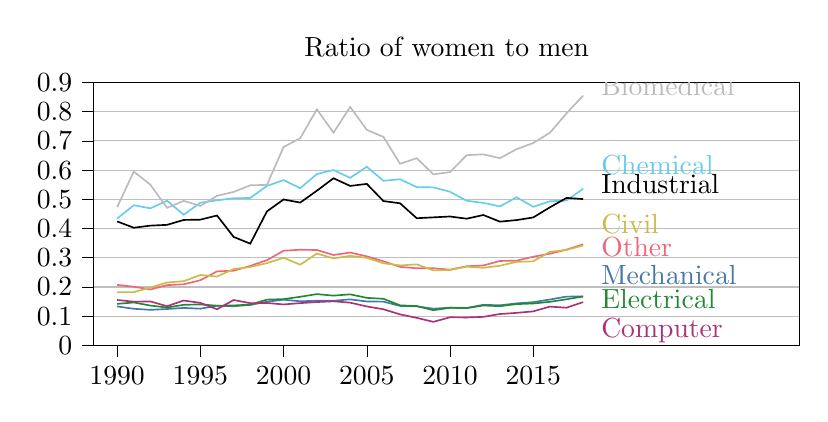
\begin{tikzpicture}

\definecolor{color0}{rgb}{0.266666666666667,0.466666666666667,0.666666666666667}
\definecolor{color1}{rgb}{0.933333333333333,0.4,0.466666666666667}
\definecolor{color2}{rgb}{0.133333333333333,0.533333333333333,0.2}
\definecolor{color3}{rgb}{0.8,0.733333333333333,0.266666666666667}
\definecolor{color4}{rgb}{0.4,0.8,0.933333333333333}
\definecolor{color5}{rgb}{0.666666666666667,0.2,0.466666666666667}

\begin{axis}[
height=140pt,
tick align=outside,
tick pos=left,
title={Ratio of women to men},
width=300pt,
x grid style={white!69.0196078431373!black},
xmin=1988.6, xmax=2031,
xtick style={color=black},
xtick={1990,1995,2000,2005,2010,2015},
xticklabels={\(\displaystyle 1990\),\(\displaystyle 1995\),\(\displaystyle 2000\),\(\displaystyle 2005\),\(\displaystyle 2010\),\(\displaystyle 2015\)},
ymajorgrids,
ymin=0, ymax=0.9,
ytick style={color=black},
ytick={0,0.1,0.2,0.3,0.4,0.5,0.6,0.7,0.8,0.9},
yticklabels={\(\displaystyle 0\),\(\displaystyle 0.1\),\(\displaystyle 0.2\),\(\displaystyle 0.3\),\(\displaystyle 0.4\),\(\displaystyle 0.5\),\(\displaystyle 0.6\),\(\displaystyle 0.7\),\(\displaystyle 0.8\),\(\displaystyle 0.9\)}
]
\addplot [semithick, color0]
table {%
1990 0.133521556854248
1991 0.125428318977356
1992 0.121800899505615
1993 0.124536991119385
1994 0.1283940076828
1995 0.125721096992493
1996 0.135704159736633
1997 0.134093880653381
1998 0.138679265975952
1999 0.149649620056152
2000 0.156452298164368
2001 0.151057720184326
2002 0.15287172794342
2003 0.152811050415039
2004 0.157570838928223
2005 0.150475263595581
2006 0.149786353111267
2007 0.135184168815613
2008 0.13373064994812
2009 0.125677108764648
2010 0.129287123680115
2011 0.128005504608154
2012 0.139001965522766
2013 0.137305736541748
2014 0.143918752670288
2015 0.147996425628662
2016 0.157168388366699
2017 0.167122602462769
2018 0.167282342910767
};
\addplot [semithick, color1]
table {%
1990 0.207133769989014
1991 0.200923800468445
1992 0.191551089286804
1993 0.206375241279602
1994 0.209223508834839
1995 0.223085045814514
1996 0.253410577774048
1997 0.255735635757446
1998 0.272221565246582
1999 0.291794538497925
2000 0.324131488800049
2001 0.327505469322205
2002 0.326584935188293
2003 0.309486031532288
2004 0.317858457565308
2005 0.304843902587891
2006 0.287989020347595
2007 0.268769383430481
2008 0.264016389846802
2009 0.264185905456543
2010 0.259300589561462
2011 0.270962476730347
2012 0.273542642593384
2013 0.289090156555176
2014 0.289969205856323
2015 0.303547978401184
2016 0.313785076141357
2017 0.328002452850342
2018 0.346036434173584
};
\addplot [semithick, color2]
table {%
1990 0.142164587974548
1991 0.14699125289917
1992 0.13635516166687
1993 0.129748225212097
1994 0.138940334320068
1995 0.140307426452637
1996 0.136027097702026
1997 0.136842966079712
1998 0.13962721824646
1999 0.156737327575684
2000 0.158464670181274
2001 0.166464805603027
2002 0.175607204437256
2003 0.170428991317749
2004 0.174860715866089
2005 0.162805438041687
2006 0.159482002258301
2007 0.137158155441284
2008 0.134697079658508
2009 0.120520830154419
2010 0.128779172897339
2011 0.127724051475525
2012 0.136640310287476
2013 0.134304046630859
2014 0.141414165496826
2015 0.143487811088562
2016 0.149130344390869
2017 0.157915830612183
2018 0.167531847953796
};
\addplot [semithick, color3]
table {%
1990 0.182199239730835
1991 0.182399034500122
1992 0.198182344436646
1993 0.215372204780579
1994 0.219987392425537
1995 0.241003632545471
1996 0.235892176628113
1997 0.26132607460022
1998 0.268557786941528
1999 0.281527280807495
2000 0.300077676773071
2001 0.276347756385803
2002 0.314508080482483
2003 0.297957181930542
2004 0.30656111240387
2005 0.299785137176514
2006 0.281087040901184
2007 0.273751616477966
2008 0.27750563621521
2009 0.256733655929565
2010 0.258218050003052
2011 0.269679546356201
2012 0.265576601028442
2013 0.272735834121704
2014 0.285907864570618
2015 0.287872791290283
2016 0.320383548736572
2017 0.326789855957031
2018 0.34207284450531
};
\addplot [semithick, color4]
table {%
1990 0.434355854988098
1991 0.479647517204285
1992 0.469239592552185
1993 0.495284557342529
1994 0.447426080703735
1995 0.488406538963318
1996 0.496622443199158
1997 0.503818511962891
1998 0.504664182662964
1999 0.545890092849731
2000 0.565838098526001
2001 0.538193464279175
2002 0.586538434028625
2003 0.600490212440491
2004 0.573595881462097
2005 0.611626267433167
2006 0.56350314617157
2007 0.568941950798035
2008 0.541939496994019
2009 0.540934801101685
2010 0.526014566421509
2011 0.495244741439819
2012 0.487799882888794
2013 0.475916385650635
2014 0.507153272628784
2015 0.474493980407715
2016 0.493396639823914
2017 0.495806217193604
2018 0.536412477493286
};
\addplot [semithick, color5]
table {%
1990 0.155529260635376
1991 0.149697303771973
1992 0.150432944297791
1993 0.134165406227112
1994 0.153651118278503
1995 0.145593881607056
1996 0.123738527297974
1997 0.155402660369873
1998 0.144569516181946
1999 0.145196199417114
2000 0.14024543762207
2001 0.144772052764893
2002 0.148424863815308
2003 0.151001811027527
2004 0.146325826644897
2005 0.133470892906189
2006 0.123713374137878
2007 0.106176018714905
2008 0.0943655967712402
2009 0.0806730985641479
2010 0.0962733030319214
2011 0.0956826210021973
2012 0.0977426767349243
2013 0.107462048530579
2014 0.111381053924561
2015 0.116504907608032
2016 0.132821917533875
2017 0.129049062728882
2018 0.14827299118042
};
\addplot [semithick, white!73.3333333333333!black]
table {%
1990 0.473233461380005
1991 0.595238089561462
1992 0.549751281738281
1993 0.470833301544189
1994 0.494802474975586
1995 0.477346301078796
1996 0.512121200561523
1997 0.525316476821899
1998 0.548063039779663
1999 0.549549579620361
2000 0.679144382476807
2001 0.709468245506287
2002 0.808068513870239
2003 0.728334903717041
2004 0.816225171089172
2005 0.737945556640625
2006 0.713721036911011
2007 0.62163507938385
2008 0.640889406204224
2009 0.585684299468994
2010 0.593220353126526
2011 0.651247024536133
2012 0.654028415679932
2013 0.640931844711304
2014 0.671709537506104
2015 0.692857146263123
2016 0.72786808013916
2017 0.794380664825439
2018 0.855445623397827
};
\addplot [semithick, black]
table {%
1990 0.424391984939575
1991 0.402864456176758
1992 0.410018563270569
1993 0.412691831588745
1994 0.429512500762939
1995 0.430440425872803
1996 0.44477105140686
1997 0.371356606483459
1998 0.348366498947144
1999 0.458837747573853
2000 0.499592542648315
2001 0.488832712173462
2002 0.529606580734253
2003 0.572199702262878
2004 0.545943021774292
2005 0.552849531173706
2006 0.494150638580322
2007 0.486431121826172
2008 0.43541145324707
2010 0.441269874572754
2011 0.433761596679688
2012 0.446334600448608
2013 0.423632144927979
2014 0.429048418998718
2015 0.438001275062561
2016 0.472658514976501
2017 0.504892349243164
2018 0.50092625617981
};
\draw (axis cs:2018.5,0.207282356402628) node[
  anchor=base west,
  text=color0,
  rotate=0.0
]{Mechanical};
\draw (axis cs:2018.5,0.306036399169415) node[
  anchor=base west,
  text=color1,
  rotate=0.0
]{Other};
\draw (axis cs:2018.5,0.127531854648419) node[
  anchor=base west,
  text=color2,
  rotate=0.0
]{Electrical};
\draw (axis cs:2018.5,0.382072882158069) node[
  anchor=base west,
  text=color3,
  rotate=0.0
]{Civil};
\draw (axis cs:2018.5,0.586412544285527) node[
  anchor=base west,
  text=color4,
  rotate=0.0
]{Chemical};
\draw (axis cs:2018.5,0.0282730550063961) node[
  anchor=base west,
  text=color5,
  rotate=0.0
]{Computer};
\draw (axis cs:2018.5,0.855445544554455) node[
  anchor=base west,
  text=white!73.3333333333333!black,
  rotate=0.0
]{Biomedical};
\draw (axis cs:2018.5,0.520926170944694) node[
  anchor=base west,
  text=black,
  rotate=0.0
]{Industrial};
\end{axis}

\end{tikzpicture}

\vspace{0.1cm}
\begin{tikzpicture}
% This file was created by tikzplotlib v0.9.2.
\definecolor{color0}{rgb}{0.266666666666667,0.466666666666667,0.666666666666667}
\definecolor{color1}{rgb}{0.933333333333333,0.4,0.466666666666667}
\definecolor{color2}{rgb}{0.133333333333333,0.533333333333333,0.2}
\definecolor{color3}{rgb}{0.8,0.733333333333333,0.266666666666667}
\definecolor{color4}{rgb}{0.4,0.8,0.933333333333333}
\definecolor{color5}{rgb}{0.666666666666667,0.2,0.466666666666667}

\begin{groupplot}[group style={group size=2 by 1, group name=my plots, horizontal sep=0.8cm}]
\nextgroupplot[
height=90pt, width=160pt,
legend style={at={(2.02, 0.5)},anchor=west,},
reverse legend,
tick align=outside,
tick pos=left,
x grid style={white!69.0196078431373!black},
xlabel={Women},
xmin=1988.6, xmax=2019.4,
xtick style={color=black},
xtick={1990,2000,2010},
xticklabels={\(\displaystyle 1990\),\(\displaystyle 2000\),\(\displaystyle 2010\)},
ymajorgrids,
ymin=0, ymax=28.9737,
ytick style={color=black}
]
\path [draw=color0, fill=color0]
(axis cs:1990,1.702)
--(axis cs:1990,0)
--(axis cs:1991,0)
--(axis cs:1992,0)
--(axis cs:1993,0)
--(axis cs:1994,0)
--(axis cs:1995,0)
--(axis cs:1996,0)
--(axis cs:1997,0)
--(axis cs:1998,0)
--(axis cs:1999,0)
--(axis cs:2000,0)
--(axis cs:2001,0)
--(axis cs:2002,0)
--(axis cs:2003,0)
--(axis cs:2004,0)
--(axis cs:2005,0)
--(axis cs:2006,0)
--(axis cs:2007,0)
--(axis cs:2008,0)
--(axis cs:2009,0)
--(axis cs:2010,0)
--(axis cs:2011,0)
--(axis cs:2012,0)
--(axis cs:2013,0)
--(axis cs:2014,0)
--(axis cs:2015,0)
--(axis cs:2016,0)
--(axis cs:2017,0)
--(axis cs:2018,0)
--(axis cs:2018,5.117)
--(axis cs:2018,5.117)
--(axis cs:2017,4.704)
--(axis cs:2016,4.043)
--(axis cs:2015,3.468)
--(axis cs:2014,3.118)
--(axis cs:2013,2.703)
--(axis cs:2012,2.56)
--(axis cs:2011,2.22)
--(axis cs:2010,2.16)
--(axis cs:2009,1.972)
--(axis cs:2008,2.087)
--(axis cs:2007,2.011)
--(axis cs:2006,2.103)
--(axis cs:2005,1.947)
--(axis cs:2004,1.946)
--(axis cs:2003,1.851)
--(axis cs:2002,1.762)
--(axis cs:2001,1.721)
--(axis cs:2000,1.764)
--(axis cs:1999,1.687)
--(axis cs:1998,1.617)
--(axis cs:1997,1.622)
--(axis cs:1996,1.721)
--(axis cs:1995,1.678)
--(axis cs:1994,1.726)
--(axis cs:1993,1.614)
--(axis cs:1992,1.542)
--(axis cs:1991,1.574)
--(axis cs:1990,1.702)
--cycle;

\path [draw=color1, fill=color1]
(axis cs:1990,3.81)
--(axis cs:1990,1.702)
--(axis cs:1991,1.574)
--(axis cs:1992,1.542)
--(axis cs:1993,1.614)
--(axis cs:1994,1.726)
--(axis cs:1995,1.678)
--(axis cs:1996,1.721)
--(axis cs:1997,1.622)
--(axis cs:1998,1.617)
--(axis cs:1999,1.687)
--(axis cs:2000,1.764)
--(axis cs:2001,1.721)
--(axis cs:2002,1.762)
--(axis cs:2003,1.851)
--(axis cs:2004,1.946)
--(axis cs:2005,1.947)
--(axis cs:2006,2.103)
--(axis cs:2007,2.011)
--(axis cs:2008,2.087)
--(axis cs:2009,1.972)
--(axis cs:2010,2.16)
--(axis cs:2011,2.22)
--(axis cs:2012,2.56)
--(axis cs:2013,2.703)
--(axis cs:2014,3.118)
--(axis cs:2015,3.468)
--(axis cs:2016,4.043)
--(axis cs:2017,4.704)
--(axis cs:2018,5.117)
--(axis cs:2018,10.783)
--(axis cs:2018,10.783)
--(axis cs:2017,10.057)
--(axis cs:2016,8.896)
--(axis cs:2015,7.857)
--(axis cs:2014,7.168)
--(axis cs:2013,6.532)
--(axis cs:2012,6.098)
--(axis cs:2011,5.5)
--(axis cs:2010,5.178)
--(axis cs:2009,4.826)
--(axis cs:2008,4.79)
--(axis cs:2007,4.61)
--(axis cs:2006,4.834)
--(axis cs:2005,4.565)
--(axis cs:2004,4.582)
--(axis cs:2003,4.386)
--(axis cs:2002,4.214)
--(axis cs:2001,4.1)
--(axis cs:2000,4.171)
--(axis cs:1999,3.874)
--(axis cs:1998,3.77)
--(axis cs:1997,3.673)
--(axis cs:1996,3.82)
--(axis cs:1995,3.574)
--(axis cs:1994,3.577)
--(axis cs:1993,3.498)
--(axis cs:1992,3.324)
--(axis cs:1991,3.575)
--(axis cs:1990,3.81)
--cycle;

\path [draw=color2, fill=color2]
(axis cs:1990,6.42)
--(axis cs:1990,3.81)
--(axis cs:1991,3.575)
--(axis cs:1992,3.324)
--(axis cs:1993,3.498)
--(axis cs:1994,3.577)
--(axis cs:1995,3.574)
--(axis cs:1996,3.82)
--(axis cs:1997,3.673)
--(axis cs:1998,3.77)
--(axis cs:1999,3.874)
--(axis cs:2000,4.171)
--(axis cs:2001,4.1)
--(axis cs:2002,4.214)
--(axis cs:2003,4.386)
--(axis cs:2004,4.582)
--(axis cs:2005,4.565)
--(axis cs:2006,4.834)
--(axis cs:2007,4.61)
--(axis cs:2008,4.79)
--(axis cs:2009,4.826)
--(axis cs:2010,5.178)
--(axis cs:2011,5.5)
--(axis cs:2012,6.098)
--(axis cs:2013,6.532)
--(axis cs:2014,7.168)
--(axis cs:2015,7.857)
--(axis cs:2016,8.896)
--(axis cs:2017,10.057)
--(axis cs:2018,10.783)
--(axis cs:2018,13.268)
--(axis cs:2018,13.268)
--(axis cs:2017,12.427)
--(axis cs:2016,10.988)
--(axis cs:2015,9.742)
--(axis cs:2014,8.932)
--(axis cs:2013,8.1)
--(axis cs:2012,7.602)
--(axis cs:2011,6.848)
--(axis cs:2010,6.524)
--(axis cs:2009,6.131)
--(axis cs:2008,6.311)
--(axis cs:2007,6.25)
--(axis cs:2006,6.817)
--(axis cs:2005,6.624)
--(axis cs:2004,6.78)
--(axis cs:2003,6.432)
--(axis cs:2002,6.224)
--(axis cs:2001,6.024)
--(axis cs:2000,5.971)
--(axis cs:1999,5.613)
--(axis cs:1998,5.388)
--(axis cs:1997,5.308)
--(axis cs:1996,5.51)
--(axis cs:1995,5.445)
--(axis cs:1994,5.528)
--(axis cs:1993,5.503)
--(axis cs:1992,5.514)
--(axis cs:1991,6.069)
--(axis cs:1990,6.42)
--cycle;

\path [draw=color3, fill=color3]
(axis cs:1990,7.55)
--(axis cs:1990,6.42)
--(axis cs:1991,6.069)
--(axis cs:1992,5.514)
--(axis cs:1993,5.503)
--(axis cs:1994,5.528)
--(axis cs:1995,5.445)
--(axis cs:1996,5.51)
--(axis cs:1997,5.308)
--(axis cs:1998,5.388)
--(axis cs:1999,5.613)
--(axis cs:2000,5.971)
--(axis cs:2001,6.024)
--(axis cs:2002,6.224)
--(axis cs:2003,6.432)
--(axis cs:2004,6.78)
--(axis cs:2005,6.624)
--(axis cs:2006,6.817)
--(axis cs:2007,6.25)
--(axis cs:2008,6.311)
--(axis cs:2009,6.131)
--(axis cs:2010,6.524)
--(axis cs:2011,6.848)
--(axis cs:2012,7.602)
--(axis cs:2013,8.1)
--(axis cs:2014,8.932)
--(axis cs:2015,9.742)
--(axis cs:2016,10.988)
--(axis cs:2017,12.427)
--(axis cs:2018,13.268)
--(axis cs:2018,16.882)
--(axis cs:2018,16.882)
--(axis cs:2017,15.823)
--(axis cs:2016,14.262)
--(axis cs:2015,12.638)
--(axis cs:2014,11.886)
--(axis cs:2013,11)
--(axis cs:2012,10.347)
--(axis cs:2011,9.575)
--(axis cs:2010,8.912)
--(axis cs:2009,8.39)
--(axis cs:2008,8.634)
--(axis cs:2007,8.388)
--(axis cs:2006,8.865)
--(axis cs:2005,8.578)
--(axis cs:2004,8.677)
--(axis cs:2003,8.299)
--(axis cs:2002,8.123)
--(axis cs:2001,7.731)
--(axis cs:2000,7.902)
--(axis cs:1999,7.707)
--(axis cs:1998,7.537)
--(axis cs:1997,7.523)
--(axis cs:1996,7.575)
--(axis cs:1995,7.414)
--(axis cs:1994,7.267)
--(axis cs:1993,7.103)
--(axis cs:1992,6.866)
--(axis cs:1991,7.211)
--(axis cs:1990,7.55)
--cycle;

\path [draw=color4, fill=color4]
(axis cs:1990,8.612)
--(axis cs:1990,7.55)
--(axis cs:1991,7.211)
--(axis cs:1992,6.866)
--(axis cs:1993,7.103)
--(axis cs:1994,7.267)
--(axis cs:1995,7.414)
--(axis cs:1996,7.575)
--(axis cs:1997,7.523)
--(axis cs:1998,7.537)
--(axis cs:1999,7.707)
--(axis cs:2000,7.902)
--(axis cs:2001,7.731)
--(axis cs:2002,8.123)
--(axis cs:2003,8.299)
--(axis cs:2004,8.677)
--(axis cs:2005,8.578)
--(axis cs:2006,8.865)
--(axis cs:2007,8.388)
--(axis cs:2008,8.634)
--(axis cs:2009,8.39)
--(axis cs:2010,8.912)
--(axis cs:2011,9.575)
--(axis cs:2012,10.347)
--(axis cs:2013,11)
--(axis cs:2014,11.886)
--(axis cs:2015,12.638)
--(axis cs:2016,14.262)
--(axis cs:2017,15.823)
--(axis cs:2018,16.882)
--(axis cs:2018,20.97)
--(axis cs:2018,20.97)
--(axis cs:2017,19.488)
--(axis cs:2016,17.587)
--(axis cs:2015,15.568)
--(axis cs:2014,14.651)
--(axis cs:2013,13.48)
--(axis cs:2012,12.706)
--(axis cs:2011,11.71)
--(axis cs:2010,10.934)
--(axis cs:2009,10.207)
--(axis cs:2008,10.372)
--(axis cs:2007,10.055)
--(axis cs:2006,10.48)
--(axis cs:2005,10.293)
--(axis cs:2004,10.454)
--(axis cs:2003,10.259)
--(axis cs:2002,10.197)
--(axis cs:2001,9.739)
--(axis cs:2000,10.042)
--(axis cs:1999,9.872)
--(axis cs:1998,9.701)
--(axis cs:1997,9.766)
--(axis cs:1996,9.707)
--(axis cs:1995,9.394)
--(axis cs:1994,8.901)
--(axis cs:1993,8.626)
--(axis cs:1992,8.094)
--(axis cs:1991,8.354)
--(axis cs:1990,8.612)
--cycle;

\path [draw=color5, fill=color5]
(axis cs:1990,8.875)
--(axis cs:1990,8.612)
--(axis cs:1991,8.354)
--(axis cs:1992,8.094)
--(axis cs:1993,8.626)
--(axis cs:1994,8.901)
--(axis cs:1995,9.394)
--(axis cs:1996,9.707)
--(axis cs:1997,9.766)
--(axis cs:1998,9.701)
--(axis cs:1999,9.872)
--(axis cs:2000,10.042)
--(axis cs:2001,9.739)
--(axis cs:2002,10.197)
--(axis cs:2003,10.259)
--(axis cs:2004,10.454)
--(axis cs:2005,10.293)
--(axis cs:2006,10.48)
--(axis cs:2007,10.055)
--(axis cs:2008,10.372)
--(axis cs:2009,10.207)
--(axis cs:2010,10.934)
--(axis cs:2011,11.71)
--(axis cs:2012,12.706)
--(axis cs:2013,13.48)
--(axis cs:2014,14.651)
--(axis cs:2015,15.568)
--(axis cs:2016,17.587)
--(axis cs:2017,19.488)
--(axis cs:2018,20.97)
--(axis cs:2018,22.245)
--(axis cs:2018,22.245)
--(axis cs:2017,20.476)
--(axis cs:2016,18.47)
--(axis cs:2015,16.252)
--(axis cs:2014,15.247)
--(axis cs:2013,13.997)
--(axis cs:2012,13.152)
--(axis cs:2011,12.12)
--(axis cs:2010,11.337)
--(axis cs:2009,10.533)
--(axis cs:2008,10.784)
--(axis cs:2007,10.557)
--(axis cs:2006,11.117)
--(axis cs:2005,11.134)
--(axis cs:2004,11.37)
--(axis cs:2003,11.186)
--(axis cs:2002,10.932)
--(axis cs:2001,10.387)
--(axis cs:2000,10.602)
--(axis cs:1999,10.342)
--(axis cs:1998,10.099)
--(axis cs:1997,10.15)
--(axis cs:1996,9.989)
--(axis cs:1995,9.698)
--(axis cs:1994,9.204)
--(axis cs:1993,8.884)
--(axis cs:1992,8.372)
--(axis cs:1991,8.626)
--(axis cs:1990,8.875)
--cycle;

\path [draw=white!73.3333333333333!black, fill=white!73.3333333333333!black]
(axis cs:1990,9.096)
--(axis cs:1990,8.875)
--(axis cs:1991,8.626)
--(axis cs:1992,8.372)
--(axis cs:1993,8.884)
--(axis cs:1994,9.204)
--(axis cs:1995,9.698)
--(axis cs:1996,9.989)
--(axis cs:1997,10.15)
--(axis cs:1998,10.099)
--(axis cs:1999,10.342)
--(axis cs:2000,10.602)
--(axis cs:2001,10.387)
--(axis cs:2002,10.932)
--(axis cs:2003,11.186)
--(axis cs:2004,11.37)
--(axis cs:2005,11.134)
--(axis cs:2006,11.117)
--(axis cs:2007,10.557)
--(axis cs:2008,10.784)
--(axis cs:2009,10.533)
--(axis cs:2010,11.337)
--(axis cs:2011,12.12)
--(axis cs:2012,13.152)
--(axis cs:2013,13.997)
--(axis cs:2014,15.247)
--(axis cs:2015,16.252)
--(axis cs:2016,18.47)
--(axis cs:2017,20.476)
--(axis cs:2018,22.245)
--(axis cs:2018,25.701)
--(axis cs:2018,25.701)
--(axis cs:2017,23.586)
--(axis cs:2016,21.249)
--(axis cs:2015,18.677)
--(axis cs:2014,17.467)
--(axis cs:2013,15.923)
--(axis cs:2012,14.946)
--(axis cs:2011,13.739)
--(axis cs:2010,12.772)
--(axis cs:2009,11.924)
--(axis cs:2008,12.11)
--(axis cs:2007,11.804)
--(axis cs:2006,12.381)
--(axis cs:2005,12.19)
--(axis cs:2004,12.356)
--(axis cs:2003,11.934)
--(axis cs:2002,11.593)
--(axis cs:2001,10.934)
--(axis cs:2000,11.11)
--(axis cs:1999,10.708)
--(axis cs:1998,10.481)
--(axis cs:1997,10.482)
--(axis cs:1996,10.327)
--(axis cs:1995,9.993)
--(axis cs:1994,9.442)
--(axis cs:1993,9.11)
--(axis cs:1992,8.593)
--(axis cs:1991,8.876)
--(axis cs:1990,9.096)
--cycle;

\path [draw=black, fill=black]
(axis cs:1990,10.3)
--(axis cs:1990,9.096)
--(axis cs:1991,8.876)
--(axis cs:1992,8.593)
--(axis cs:1993,9.11)
--(axis cs:1994,9.442)
--(axis cs:1995,9.993)
--(axis cs:1996,10.327)
--(axis cs:1997,10.482)
--(axis cs:1998,10.481)
--(axis cs:1999,10.708)
--(axis cs:2000,11.11)
--(axis cs:2001,10.934)
--(axis cs:2002,11.593)
--(axis cs:2003,11.934)
--(axis cs:2004,12.356)
--(axis cs:2005,12.19)
--(axis cs:2006,12.381)
--(axis cs:2007,11.804)
--(axis cs:2008,12.11)
--(axis cs:2009,11.924)
--(axis cs:2010,12.772)
--(axis cs:2011,13.739)
--(axis cs:2012,14.946)
--(axis cs:2013,15.923)
--(axis cs:2014,17.467)
--(axis cs:2015,18.677)
--(axis cs:2016,21.249)
--(axis cs:2017,23.586)
--(axis cs:2018,25.701)
--(axis cs:2018,27.594)
--(axis cs:2018,27.594)
--(axis cs:2017,25.392)
--(axis cs:2016,22.874)
--(axis cs:2015,20.097)
--(axis cs:2014,18.752)
--(axis cs:2013,17.038)
--(axis cs:2012,16.048)
--(axis cs:2011,14.718)
--(axis cs:2010,13.745)
--(axis cs:2009,12.842)
--(axis cs:2008,12.983)
--(axis cs:2007,12.754)
--(axis cs:2006,13.437)
--(axis cs:2005,13.325)
--(axis cs:2004,13.372)
--(axis cs:2003,12.358)
--(axis cs:2002,12.872)
--(axis cs:2001,12.094)
--(axis cs:2000,12.336)
--(axis cs:1999,11.845)
--(axis cs:1998,11.462)
--(axis cs:1997,11.514)
--(axis cs:1996,11.386)
--(axis cs:1995,10.98)
--(axis cs:1994,10.42)
--(axis cs:1993,10.105)
--(axis cs:1992,9.698)
--(axis cs:1991,9.973)
--(axis cs:1990,10.3)
--cycle;

\addplot [semithick, color0]
table {%
1990 1.70200002193451
1991 1.57400000095367
1992 1.54200005531311
1993 1.6139999628067
1994 1.72599995136261
1995 1.67799997329712
1996 1.72099995613098
1997 1.62199997901917
1998 1.61699998378754
2000 1.76400005817413
2001 1.72099995613098
2002 1.76199996471405
2004 1.94599997997284
2005 1.94700002670288
2006 2.1029999256134
2007 2.01099991798401
2008 2.08699989318848
2009 1.97200000286102
2010 2.16000008583069
2011 2.22000002861023
2012 2.55999994277954
2013 2.70300006866455
2014 3.11800003051758
2015 3.46799993515015
2016 4.04300022125244
2017 4.7039999961853
2018 5.11700010299683
};
\addplot [semithick, color1]
table {%
1990 3.80999994277954
1991 3.57500004768372
1992 3.32399988174438
1993 3.49799990653992
1994 3.57699990272522
1995 3.57399988174438
1996 3.8199999332428
1997 3.67300009727478
1999 3.87400007247925
2000 4.1710000038147
2001 4.09999990463257
2002 4.21400022506714
2003 4.38600015640259
2004 4.58199977874756
2005 4.56500005722046
2006 4.83400011062622
2007 4.6100001335144
2008 4.78999996185303
2009 4.82600021362305
2010 5.17799997329712
2011 5.5
2012 6.09800004959106
2013 6.53200006484985
2014 7.16800022125244
2015 7.85699987411499
2016 8.89599990844727
2017 10.0570001602173
2018 10.7829999923706
};
\addplot [semithick, color2]
table {%
1990 6.42000007629395
1991 6.06899976730347
1992 5.51399993896484
1993 5.50299978256226
1994 5.52799987792969
1995 5.44500017166138
1996 5.51000022888184
1997 5.30800008773804
1998 5.38800001144409
1999 5.61299991607666
2000 5.97100019454956
2001 6.02400016784668
2003 6.43200016021729
2004 6.78000020980835
2005 6.62400007247925
2006 6.81699991226196
2007 6.25
2008 6.31099987030029
2009 6.13100004196167
2010 6.52400016784668
2011 6.84800004959106
2012 7.60200023651123
2013 8.10000038146973
2014 8.93200016021729
2015 9.74199962615967
2016 10.9879999160767
2017 12.4270000457764
2018 13.2679996490479
};
\addplot [semithick, color3]
table {%
1990 7.55000019073486
1992 6.86600017547607
1993 7.10300016403198
1994 7.26700019836426
1995 7.41400003433228
1996 7.57499980926514
1997 7.52299976348877
1998 7.53700017929077
1999 7.70699977874756
2000 7.90199995040894
2001 7.73099994659424
2002 8.1230001449585
2003 8.29899978637695
2004 8.67700004577637
2005 8.57800006866455
2006 8.86499977111816
2007 8.38799953460693
2008 8.63399982452393
2009 8.39000034332275
2010 8.91199970245361
2011 9.57499980926514
2012 10.3470001220703
2013 11
2014 11.8859996795654
2015 12.6379995346069
2016 14.2620000839233
2017 15.8229999542236
2018 16.8819999694824
};
\addplot [semithick, color4]
table {%
1990 8.61200046539307
1992 8.0939998626709
1993 8.62600040435791
1994 8.90100002288818
1995 9.39400005340576
1996 9.70699977874756
1997 9.76599979400635
1998 9.70100021362305
2000 10.0419998168945
2001 9.73900032043457
2002 10.1969995498657
2003 10.2589998245239
2004 10.4540004730225
2005 10.2930002212524
2006 10.4799995422363
2007 10.0550003051758
2008 10.3719997406006
2009 10.2069997787476
2010 10.9340000152588
2011 11.710000038147
2012 12.706000328064
2013 13.4799995422363
2014 14.6510000228882
2015 15.5679998397827
2016 17.5869998931885
2017 19.488000869751
2018 20.9699993133545
};
\addplot [semithick, color5]
table {%
1990 8.875
1992 8.37199974060059
1993 8.88399982452393
1994 9.20400047302246
1995 9.69799995422363
1996 9.98900032043457
1997 10.1499996185303
1998 10.0989999771118
1999 10.3420000076294
2000 10.6020002365112
2001 10.3870000839233
2002 10.9320001602173
2003 11.1859998703003
2004 11.3699998855591
2005 11.1339998245239
2006 11.1169996261597
2007 10.5570001602173
2008 10.7840003967285
2009 10.5329999923706
2010 11.3369998931885
2011 12.1199998855591
2012 13.1520004272461
2013 13.9969997406006
2014 15.2469997406006
2015 16.2520008087158
2016 18.4699993133545
2017 20.4759998321533
2018 22.2450008392334
};
\addplot [semithick, white!73.3333333333333!black]
table {%
1990 9.0959997177124
1991 8.87600040435791
1992 8.5930004119873
1993 9.10999965667725
1994 9.44200038909912
1995 9.99300003051758
1996 10.3269996643066
1997 10.4820003509521
1998 10.4809999465942
1999 10.7080001831055
2000 11.1099996566772
2001 10.9340000152588
2002 11.5930004119873
2003 11.9340000152588
2004 12.3559999465942
2005 12.1899995803833
2006 12.3809995651245
2007 11.8039999008179
2008 12.1099996566772
2009 11.923999786377
2010 12.7720003128052
2011 13.7390003204346
2012 14.9460000991821
2013 15.9230003356934
2014 17.4669990539551
2015 18.6770000457764
2016 21.2490005493164
2017 23.5860004425049
2018 25.701000213623
};
\addplot [semithick, black]
table {%
1990 10.3000001907349
1991 9.97299957275391
1992 9.69799995422363
1993 10.1049995422363
1994 10.4200000762939
1995 10.9799995422363
1996 11.3859996795654
1997 11.5139999389648
1998 11.4619998931885
1999 11.8450002670288
2000 12.3360004425049
2001 12.0939998626709
2002 12.8719997406006
2003 12.3579998016357
2004 13.3719997406006
2005 13.3249998092651
2006 13.4370002746582
2007 12.753999710083
2008 12.9829998016357
2009 12.8420000076294
2010 13.7449998855591
2011 14.7180004119873
2012 16.0480003356934
2013 17.0380001068115
2014 18.7520008087158
2015 20.0970001220703
2016 22.8740005493164
2017 25.3920001983643
2018 27.5939998626709
};

\nextgroupplot[
height=90pt, width=160pt,
legend style={at={(2.02, 0.5)},anchor=west,},
reverse legend,
tick align=outside,
tick pos=left,
x grid style={white!69.0196078431373!black},
xlabel={Men},
xmin=1988.6, xmax=2019.4,
xtick style={color=black},
xtick={1990,2000,2010},
xticklabels={\(\displaystyle 1990\),\(\displaystyle 2000\),\(\displaystyle 2010\)},
ymajorgrids,
ymin=0, ymax=101.22,
ytick style={color=black}
]
\path [draw=color0, fill=color0]
(axis cs:1990,12.747)
--(axis cs:1990,0)
--(axis cs:1991,0)
--(axis cs:1992,0)
--(axis cs:1993,0)
--(axis cs:1994,0)
--(axis cs:1995,0)
--(axis cs:1996,0)
--(axis cs:1997,0)
--(axis cs:1998,0)
--(axis cs:1999,0)
--(axis cs:2000,0)
--(axis cs:2001,0)
--(axis cs:2002,0)
--(axis cs:2003,0)
--(axis cs:2004,0)
--(axis cs:2005,0)
--(axis cs:2006,0)
--(axis cs:2007,0)
--(axis cs:2008,0)
--(axis cs:2009,0)
--(axis cs:2010,0)
--(axis cs:2011,0)
--(axis cs:2012,0)
--(axis cs:2013,0)
--(axis cs:2014,0)
--(axis cs:2015,0)
--(axis cs:2016,0)
--(axis cs:2017,0)
--(axis cs:2018,0)
--(axis cs:2018,30.589)
--(axis cs:2018,30.589)
--(axis cs:2017,28.147)
--(axis cs:2016,25.724)
--(axis cs:2015,23.433)
--(axis cs:2014,21.665)
--(axis cs:2013,19.686)
--(axis cs:2012,18.417)
--(axis cs:2011,17.343)
--(axis cs:2010,16.707)
--(axis cs:2009,15.691)
--(axis cs:2008,15.606)
--(axis cs:2007,14.876)
--(axis cs:2006,14.04)
--(axis cs:2005,12.939)
--(axis cs:2004,12.35)
--(axis cs:2003,12.113)
--(axis cs:2002,11.526)
--(axis cs:2001,11.393)
--(axis cs:2000,11.275)
--(axis cs:1999,11.273)
--(axis cs:1998,11.66)
--(axis cs:1997,12.096)
--(axis cs:1996,12.682)
--(axis cs:1995,13.347)
--(axis cs:1994,13.443)
--(axis cs:1993,12.96)
--(axis cs:1992,12.66)
--(axis cs:1991,12.549)
--(axis cs:1990,12.747)
--cycle;

\path [draw=color1, fill=color1]
(axis cs:1990,22.924)
--(axis cs:1990,12.747)
--(axis cs:1991,12.549)
--(axis cs:1992,12.66)
--(axis cs:1993,12.96)
--(axis cs:1994,13.443)
--(axis cs:1995,13.347)
--(axis cs:1996,12.682)
--(axis cs:1997,12.096)
--(axis cs:1998,11.66)
--(axis cs:1999,11.273)
--(axis cs:2000,11.275)
--(axis cs:2001,11.393)
--(axis cs:2002,11.526)
--(axis cs:2003,12.113)
--(axis cs:2004,12.35)
--(axis cs:2005,12.939)
--(axis cs:2006,14.04)
--(axis cs:2007,14.876)
--(axis cs:2008,15.606)
--(axis cs:2009,15.691)
--(axis cs:2010,16.707)
--(axis cs:2011,17.343)
--(axis cs:2012,18.417)
--(axis cs:2013,19.686)
--(axis cs:2014,21.665)
--(axis cs:2015,23.433)
--(axis cs:2016,25.724)
--(axis cs:2017,28.147)
--(axis cs:2018,30.589)
--(axis cs:2018,46.963)
--(axis cs:2018,46.963)
--(axis cs:2017,44.467)
--(axis cs:2016,41.19)
--(axis cs:2015,37.892)
--(axis cs:2014,35.632)
--(axis cs:2013,32.931)
--(axis cs:2012,31.351)
--(axis cs:2011,29.448)
--(axis cs:2010,28.346)
--(axis cs:2009,26.494)
--(axis cs:2008,25.844)
--(axis cs:2007,24.546)
--(axis cs:2006,23.523)
--(axis cs:2005,21.527)
--(axis cs:2004,20.643)
--(axis cs:2003,20.304)
--(axis cs:2002,19.034)
--(axis cs:2001,18.657)
--(axis cs:2000,18.701)
--(axis cs:1999,18.768)
--(axis cs:1998,19.569)
--(axis cs:1997,20.116)
--(axis cs:1996,20.965)
--(axis cs:1995,21.846)
--(axis cs:1994,22.29)
--(axis cs:1993,22.089)
--(axis cs:1992,21.963)
--(axis cs:1991,22.508)
--(axis cs:1990,22.924)
--cycle;

\path [draw=color2, fill=color2]
(axis cs:1990,41.283)
--(axis cs:1990,22.924)
--(axis cs:1991,22.508)
--(axis cs:1992,21.963)
--(axis cs:1993,22.089)
--(axis cs:1994,22.29)
--(axis cs:1995,21.846)
--(axis cs:1996,20.965)
--(axis cs:1997,20.116)
--(axis cs:1998,19.569)
--(axis cs:1999,18.768)
--(axis cs:2000,18.701)
--(axis cs:2001,18.657)
--(axis cs:2002,19.034)
--(axis cs:2003,20.304)
--(axis cs:2004,20.643)
--(axis cs:2005,21.527)
--(axis cs:2006,23.523)
--(axis cs:2007,24.546)
--(axis cs:2008,25.844)
--(axis cs:2009,26.494)
--(axis cs:2010,28.346)
--(axis cs:2011,29.448)
--(axis cs:2012,31.351)
--(axis cs:2013,32.931)
--(axis cs:2014,35.632)
--(axis cs:2015,37.892)
--(axis cs:2016,41.19)
--(axis cs:2017,44.467)
--(axis cs:2018,46.963)
--(axis cs:2018,61.796)
--(axis cs:2018,61.796)
--(axis cs:2017,59.475)
--(axis cs:2016,55.218)
--(axis cs:2015,51.029)
--(axis cs:2014,48.106)
--(axis cs:2013,44.606)
--(axis cs:2012,42.358)
--(axis cs:2011,40.002)
--(axis cs:2010,38.798)
--(axis cs:2009,37.322)
--(axis cs:2008,37.136)
--(axis cs:2007,36.503)
--(axis cs:2006,35.957)
--(axis cs:2005,34.174)
--(axis cs:2004,33.213)
--(axis cs:2003,32.309)
--(axis cs:2002,30.48)
--(axis cs:2001,30.215)
--(axis cs:2000,30.06)
--(axis cs:1999,29.863)
--(axis cs:1998,31.157)
--(axis cs:1997,32.064)
--(axis cs:1996,33.389)
--(axis cs:1995,35.181)
--(axis cs:1994,36.332)
--(axis cs:1993,37.542)
--(axis cs:1992,38.024)
--(axis cs:1991,39.475)
--(axis cs:1990,41.283)
--cycle;

\path [draw=color3, fill=color3]
(axis cs:1990,47.485)
--(axis cs:1990,41.283)
--(axis cs:1991,39.475)
--(axis cs:1992,38.024)
--(axis cs:1993,37.542)
--(axis cs:1994,36.332)
--(axis cs:1995,35.181)
--(axis cs:1996,33.389)
--(axis cs:1997,32.064)
--(axis cs:1998,31.157)
--(axis cs:1999,29.863)
--(axis cs:2000,30.06)
--(axis cs:2001,30.215)
--(axis cs:2002,30.48)
--(axis cs:2003,32.309)
--(axis cs:2004,33.213)
--(axis cs:2005,34.174)
--(axis cs:2006,35.957)
--(axis cs:2007,36.503)
--(axis cs:2008,37.136)
--(axis cs:2009,37.322)
--(axis cs:2010,38.798)
--(axis cs:2011,40.002)
--(axis cs:2012,42.358)
--(axis cs:2013,44.606)
--(axis cs:2014,48.106)
--(axis cs:2015,51.029)
--(axis cs:2016,55.218)
--(axis cs:2017,59.475)
--(axis cs:2018,61.796)
--(axis cs:2018,72.361)
--(axis cs:2018,72.361)
--(axis cs:2017,69.867)
--(axis cs:2016,65.437)
--(axis cs:2015,61.089)
--(axis cs:2014,58.438)
--(axis cs:2013,55.239)
--(axis cs:2012,52.694)
--(axis cs:2011,50.114)
--(axis cs:2010,48.046)
--(axis cs:2009,46.121)
--(axis cs:2008,45.507)
--(axis cs:2007,44.313)
--(axis cs:2006,43.243)
--(axis cs:2005,40.692)
--(axis cs:2004,39.401)
--(axis cs:2003,38.575)
--(axis cs:2002,36.518)
--(axis cs:2001,36.392)
--(axis cs:2000,36.495)
--(axis cs:1999,37.301)
--(axis cs:1998,39.159)
--(axis cs:1997,40.54)
--(axis cs:1996,42.143)
--(axis cs:1995,43.351)
--(axis cs:1994,44.237)
--(axis cs:1993,44.971)
--(axis cs:1992,44.846)
--(axis cs:1991,45.736)
--(axis cs:1990,47.485)
--cycle;

\path [draw=color4, fill=color4]
(axis cs:1990,49.93)
--(axis cs:1990,47.485)
--(axis cs:1991,45.736)
--(axis cs:1992,44.846)
--(axis cs:1993,44.971)
--(axis cs:1994,44.237)
--(axis cs:1995,43.351)
--(axis cs:1996,42.143)
--(axis cs:1997,40.54)
--(axis cs:1998,39.159)
--(axis cs:1999,37.301)
--(axis cs:2000,36.495)
--(axis cs:2001,36.392)
--(axis cs:2002,36.518)
--(axis cs:2003,38.575)
--(axis cs:2004,39.401)
--(axis cs:2005,40.692)
--(axis cs:2006,43.243)
--(axis cs:2007,44.313)
--(axis cs:2008,45.507)
--(axis cs:2009,46.121)
--(axis cs:2010,48.046)
--(axis cs:2011,50.114)
--(axis cs:2012,52.694)
--(axis cs:2013,55.239)
--(axis cs:2014,58.438)
--(axis cs:2015,61.089)
--(axis cs:2016,65.437)
--(axis cs:2017,69.867)
--(axis cs:2018,72.361)
--(axis cs:2018,79.982)
--(axis cs:2018,79.982)
--(axis cs:2017,77.259)
--(axis cs:2016,72.176)
--(axis cs:2015,67.264)
--(axis cs:2014,63.89)
--(axis cs:2013,60.45)
--(axis cs:2012,57.53)
--(axis cs:2011,54.425)
--(axis cs:2010,51.89)
--(axis cs:2009,49.48)
--(axis cs:2008,48.714)
--(axis cs:2007,47.243)
--(axis cs:2006,46.109)
--(axis cs:2005,43.496)
--(axis cs:2004,42.499)
--(axis cs:2003,41.839)
--(axis cs:2002,40.054)
--(axis cs:2001,40.123)
--(axis cs:2000,40.277)
--(axis cs:1999,41.267)
--(axis cs:1998,43.447)
--(axis cs:1997,44.992)
--(axis cs:1996,46.436)
--(axis cs:1995,47.405)
--(axis cs:1994,47.889)
--(axis cs:1993,48.046)
--(axis cs:1992,47.463)
--(axis cs:1991,48.119)
--(axis cs:1990,49.93)
--cycle;

\path [draw=color5, fill=color5]
(axis cs:1990,51.621)
--(axis cs:1990,49.93)
--(axis cs:1991,48.119)
--(axis cs:1992,47.463)
--(axis cs:1993,48.046)
--(axis cs:1994,47.889)
--(axis cs:1995,47.405)
--(axis cs:1996,46.436)
--(axis cs:1997,44.992)
--(axis cs:1998,43.447)
--(axis cs:1999,41.267)
--(axis cs:2000,40.277)
--(axis cs:2001,40.123)
--(axis cs:2002,40.054)
--(axis cs:2003,41.839)
--(axis cs:2004,42.499)
--(axis cs:2005,43.496)
--(axis cs:2006,46.109)
--(axis cs:2007,47.243)
--(axis cs:2008,48.714)
--(axis cs:2009,49.48)
--(axis cs:2010,51.89)
--(axis cs:2011,54.425)
--(axis cs:2012,57.53)
--(axis cs:2013,60.45)
--(axis cs:2014,63.89)
--(axis cs:2015,67.264)
--(axis cs:2016,72.176)
--(axis cs:2017,77.259)
--(axis cs:2018,79.982)
--(axis cs:2018,88.581)
--(axis cs:2018,88.581)
--(axis cs:2017,84.915)
--(axis cs:2016,78.824)
--(axis cs:2015,73.135)
--(axis cs:2014,69.241)
--(axis cs:2013,65.261)
--(axis cs:2012,62.093)
--(axis cs:2011,58.71)
--(axis cs:2010,56.076)
--(axis cs:2009,53.521)
--(axis cs:2008,53.08)
--(axis cs:2007,51.971)
--(axis cs:2006,51.258)
--(axis cs:2005,49.797)
--(axis cs:2004,48.759)
--(axis cs:2003,47.978)
--(axis cs:2002,45.006)
--(axis cs:2001,44.599)
--(axis cs:2000,44.27)
--(axis cs:1999,44.504)
--(axis cs:1998,46.2)
--(axis cs:1997,47.463)
--(axis cs:1996,48.715)
--(axis cs:1995,49.493)
--(axis cs:1994,49.861)
--(axis cs:1993,49.969)
--(axis cs:1992,49.311)
--(axis cs:1991,49.936)
--(axis cs:1990,51.621)
--cycle;

\path [draw=white!73.3333333333333!black, fill=white!73.3333333333333!black]
(axis cs:1990,52.088)
--(axis cs:1990,51.621)
--(axis cs:1991,49.936)
--(axis cs:1992,49.311)
--(axis cs:1993,49.969)
--(axis cs:1994,49.861)
--(axis cs:1995,49.493)
--(axis cs:1996,48.715)
--(axis cs:1997,47.463)
--(axis cs:1998,46.2)
--(axis cs:1999,44.504)
--(axis cs:2000,44.27)
--(axis cs:2001,44.599)
--(axis cs:2002,45.006)
--(axis cs:2003,47.978)
--(axis cs:2004,48.759)
--(axis cs:2005,49.797)
--(axis cs:2006,51.258)
--(axis cs:2007,51.971)
--(axis cs:2008,53.08)
--(axis cs:2009,53.521)
--(axis cs:2010,56.076)
--(axis cs:2011,58.71)
--(axis cs:2012,62.093)
--(axis cs:2013,65.261)
--(axis cs:2014,69.241)
--(axis cs:2015,73.135)
--(axis cs:2016,78.824)
--(axis cs:2017,84.915)
--(axis cs:2018,88.581)
--(axis cs:2018,92.621)
--(axis cs:2018,92.621)
--(axis cs:2017,88.83)
--(axis cs:2016,82.642)
--(axis cs:2015,76.635)
--(axis cs:2014,72.546)
--(axis cs:2013,68.266)
--(axis cs:2012,64.836)
--(axis cs:2011,61.196)
--(axis cs:2010,58.495)
--(axis cs:2009,55.896)
--(axis cs:2008,55.149)
--(axis cs:2007,53.977)
--(axis cs:2006,53.029)
--(axis cs:2005,51.228)
--(axis cs:2004,49.967)
--(axis cs:2003,49.005)
--(axis cs:2002,45.824)
--(axis cs:2001,45.37)
--(axis cs:2000,45.018)
--(axis cs:1999,45.17)
--(axis cs:1998,46.897)
--(axis cs:1997,48.095)
--(axis cs:1996,49.375)
--(axis cs:1995,50.111)
--(axis cs:1994,50.342)
--(axis cs:1993,50.449)
--(axis cs:1992,49.713)
--(axis cs:1991,50.356)
--(axis cs:1990,52.088)
--cycle;

\path [draw=black, fill=black]
(axis cs:1990,54.925)
--(axis cs:1990,52.088)
--(axis cs:1991,50.356)
--(axis cs:1992,49.713)
--(axis cs:1993,50.449)
--(axis cs:1994,50.342)
--(axis cs:1995,50.111)
--(axis cs:1996,49.375)
--(axis cs:1997,48.095)
--(axis cs:1998,46.897)
--(axis cs:1999,45.17)
--(axis cs:2000,45.018)
--(axis cs:2001,45.37)
--(axis cs:2002,45.824)
--(axis cs:2003,49.005)
--(axis cs:2004,49.967)
--(axis cs:2005,51.228)
--(axis cs:2006,53.029)
--(axis cs:2007,53.977)
--(axis cs:2008,55.149)
--(axis cs:2009,55.896)
--(axis cs:2010,58.495)
--(axis cs:2011,61.196)
--(axis cs:2012,64.836)
--(axis cs:2013,68.266)
--(axis cs:2014,72.546)
--(axis cs:2015,76.635)
--(axis cs:2016,82.642)
--(axis cs:2017,88.83)
--(axis cs:2018,92.621)
--(axis cs:2018,96.4)
--(axis cs:2018,96.4)
--(axis cs:2017,92.407)
--(axis cs:2016,86.08)
--(axis cs:2015,79.877)
--(axis cs:2014,75.541)
--(axis cs:2013,70.898)
--(axis cs:2012,67.305)
--(axis cs:2011,63.453)
--(axis cs:2010,60.7)
--(axis cs:2009,57.99)
--(axis cs:2008,57.154)
--(axis cs:2007,55.93)
--(axis cs:2006,55.166)
--(axis cs:2005,53.281)
--(axis cs:2004,51.828)
--(axis cs:2003,49.746)
--(axis cs:2002,48.239)
--(axis cs:2001,47.743)
--(axis cs:2000,47.472)
--(axis cs:1999,47.648)
--(axis cs:1998,49.713)
--(axis cs:1997,50.874)
--(axis cs:1996,51.756)
--(axis cs:1995,52.404)
--(axis cs:1994,52.619)
--(axis cs:1993,52.86)
--(axis cs:1992,52.408)
--(axis cs:1991,53.079)
--(axis cs:1990,54.925)
--cycle;

\addplot [semithick, color0]
table {%
1990 12.7469997406006
1991 12.548999786377
1992 12.6599998474121
1993 12.960000038147
1994 13.4429998397827
1995 13.3470001220703
1996 12.6820001602173
1997 12.0959997177124
1998 11.6599998474121
1999 11.2729997634888
2000 11.2749996185303
2001 11.3929996490479
2002 11.5260000228882
2003 12.1129999160767
2004 12.3500003814697
2005 12.9390001296997
2006 14.039999961853
2007 14.8760004043579
2008 15.6059999465942
2009 15.6909999847412
2010 16.7070007324219
2011 17.3430004119873
2012 18.4169998168945
2013 19.6860008239746
2014 21.6650009155273
2015 23.4330005645752
2016 25.7240009307861
2018 30.5890007019043
};
\addplot [semithick, color1]
table {%
1990 22.923999786377
1991 22.507999420166
1992 21.9629993438721
1993 22.0890007019043
1994 22.2900009155273
1995 21.8460006713867
1996 20.9650001525879
1997 20.1159992218018
1998 19.5690002441406
1999 18.7679996490479
2000 18.701000213623
2001 18.6569995880127
2002 19.0340003967285
2003 20.3040008544922
2004 20.6429996490479
2005 21.5270004272461
2006 23.5230007171631
2007 24.5459995269775
2008 25.8439998626709
2009 26.4939994812012
2010 28.3460006713867
2011 29.4479999542236
2012 31.3509998321533
2013 32.9309997558594
2014 35.6319999694824
2015 37.8919982910156
2017 44.4669990539551
2018 46.9630012512207
};
\addplot [semithick, color2]
table {%
1990 41.2830009460449
1991 39.4749984741211
1992 38.023998260498
1993 37.5419998168945
1994 36.3320007324219
1995 35.1809997558594
1996 33.3889999389648
1997 32.0639991760254
1998 31.1569995880127
1999 29.863000869751
2000 30.0599994659424
2001 30.2150001525879
2002 30.4799995422363
2003 32.3089981079102
2004 33.2130012512207
2005 34.173999786377
2006 35.9570007324219
2007 36.5029983520508
2008 37.1360015869141
2009 37.3219985961914
2010 38.7980003356934
2011 40.0019989013672
2012 42.3580017089844
2013 44.6059989929199
2014 48.1059989929199
2015 51.0289993286133
2016 55.2179985046387
2017 59.4749984741211
2018 61.7960014343262
};
\addplot [semithick, color3]
table {%
1990 47.4850006103516
1991 45.7360000610352
1992 44.8460006713867
1993 44.9710006713867
1994 44.2369995117188
1995 43.351001739502
1996 42.1430015563965
1997 40.5400009155273
1998 39.1590003967285
1999 37.3009986877441
2000 36.4949989318848
2001 36.3919982910156
2002 36.5180015563965
2003 38.5750007629395
2004 39.4010009765625
2005 40.6920013427734
2006 43.2430000305176
2007 44.3129997253418
2008 45.5069999694824
2009 46.1209983825684
2010 48.0460014343262
2011 50.1139984130859
2012 52.6940002441406
2013 55.2389984130859
2014 58.4379997253418
2015 61.0890007019043
2016 65.4369964599609
2017 69.8669967651367
2018 72.3610000610352
};
\addplot [semithick, color4]
table {%
1990 49.9300003051758
1991 48.1189994812012
1992 47.4630012512207
1993 48.0460014343262
1994 47.8889999389648
1995 47.4049987792969
1996 46.4360008239746
1997 44.992000579834
1998 43.4469985961914
1999 41.2669982910156
2000 40.2770004272461
2001 40.1230010986328
2002 40.0540008544922
2003 41.8390007019043
2004 42.4990005493164
2005 43.4959983825684
2006 46.109001159668
2007 47.2430000305176
2008 48.7140007019043
2009 49.4799995422363
2010 51.8899993896484
2011 54.4249992370605
2012 57.5299987792969
2013 60.4500007629395
2014 63.8899993896484
2015 67.2639999389648
2016 72.1760025024414
2017 77.2590026855469
2018 79.9820022583008
};
\addplot [semithick, color5]
table {%
1990 51.6209983825684
1991 49.9360008239746
1992 49.3110008239746
1993 49.9690017700195
1994 49.8610000610352
1995 49.4930000305176
1996 48.7150001525879
1998 46.2000007629395
1999 44.5040016174316
2000 44.2700004577637
2001 44.5989990234375
2002 45.0060005187988
2003 47.9780006408691
2004 48.7589988708496
2005 49.7970008850098
2006 51.257999420166
2007 51.9710006713867
2008 53.0800018310547
2009 53.5209999084473
2010 56.076000213623
2011 58.7099990844727
2012 62.0929985046387
2013 65.2610015869141
2014 69.2409973144531
2015 73.1350021362305
2016 78.8239974975586
2017 84.9150009155273
2018 88.5810012817383
};
\addplot [semithick, white!73.3333333333333!black]
table {%
1990 52.0880012512207
1991 50.3559989929199
1992 49.7130012512207
1993 50.4490013122559
1994 50.3419990539551
1995 50.1110000610352
1996 49.375
1997 48.0950012207031
1998 46.8969993591309
1999 45.1699981689453
2000 45.0180015563965
2001 45.3699989318848
2002 45.8240013122559
2003 49.0050010681152
2004 49.9669990539551
2005 51.2280006408691
2006 53.0289993286133
2007 53.9770011901855
2008 55.148998260498
2009 55.8959999084473
2010 58.4949989318848
2011 61.1959991455078
2012 64.8359985351562
2013 68.265998840332
2014 72.5459976196289
2015 76.6350021362305
2016 82.6419982910156
2017 88.8300018310547
2018 92.6210021972656
};
\addplot [semithick, black]
table {%
1990 54.9249992370605
1991 53.0789985656738
1992 52.4080009460449
1993 52.8600006103516
1994 52.6189994812012
1995 52.4039993286133
1996 51.7560005187988
1997 50.8740005493164
1998 49.7130012512207
1999 47.6479988098145
2000 47.4720001220703
2001 47.7430000305176
2002 48.2389984130859
2003 49.7459983825684
2004 51.8279991149902
2005 53.2809982299805
2006 55.1660003662109
2007 55.9300003051758
2008 57.1539993286133
2009 57.9900016784668
2010 60.7000007629395
2011 63.4529991149902
2012 67.3050003051758
2013 70.8980026245117
2014 75.5410003662109
2015 79.8769989013672
2016 86.0800018310547
2017 92.4069976806641
2018 96.4000015258789
};
\end{groupplot}




\end{tikzpicture}
\caption{Number Bachelor's degrees awarded (thousands). Source: IPEDS.}

\end{figure}
\hyperlink{intro_social_science_ratio}{\beamerbutton{Return: Social science ratio}}
}
\end{frame}

%%%%%%%%%%%%%%%%%%%%%%%%%%%%%%%%%%%%%%%%%%%%%%%%%%%%%%%%%%%%%%%%%%%%%%%%%%%%%%%%
\begin{frame}{Business}\label{app_business}
\Wider[4em]{

\begin{figure}
\setlength{\abovecaptionskip}{2pt}
\setlength{\belowcaptionskip}{-2pt}
% This file was created by tikzplotlib v0.9.2.
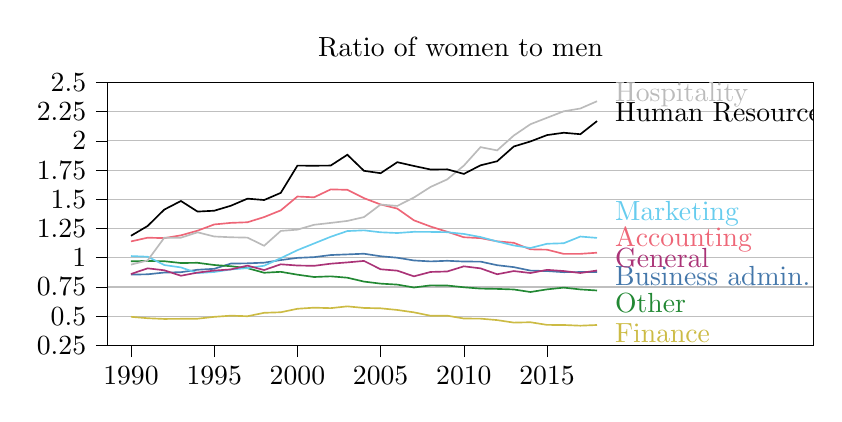
\begin{tikzpicture}

\definecolor{color0}{rgb}{0.266666666666667,0.466666666666667,0.666666666666667}
\definecolor{color1}{rgb}{0.933333333333333,0.4,0.466666666666667}
\definecolor{color2}{rgb}{0.133333333333333,0.533333333333333,0.2}
\definecolor{color3}{rgb}{0.8,0.733333333333333,0.266666666666667}
\definecolor{color4}{rgb}{0.4,0.8,0.933333333333333}
\definecolor{color5}{rgb}{0.666666666666667,0.2,0.466666666666667}

\begin{axis}[
height=140pt,
tick align=outside,
tick pos=left,
title={Ratio of women to men},
width=300pt,
x grid style={white!69.0196078431373!black},
xmin=1988.6, xmax=2031,
xtick style={color=black},
xtick={1990,1995,2000,2005,2010,2015},
xticklabels={\(\displaystyle 1990\),\(\displaystyle 1995\),\(\displaystyle 2000\),\(\displaystyle 2005\),\(\displaystyle 2010\),\(\displaystyle 2015\)},
ymajorgrids,
ymin=0.25, ymax=2.5,
ytick style={color=black},
ytick={0.25,0.5,0.75,1,1.25,1.5,1.75,2,2.25,2.5},
yticklabels={\(\displaystyle 0.25\),\(\displaystyle 0.5\),\(\displaystyle 0.75\),\(\displaystyle 1\),\(\displaystyle 1.25\),\(\displaystyle 1.5\),\(\displaystyle 1.75\),\(\displaystyle 2\),\(\displaystyle 2.25\),\(\displaystyle 2.5\)}
]
\addplot [semithick, color0]
table {%
1990 0.855923891067505
1991 0.858499646186829
1992 0.873625755310059
1993 0.876446723937988
1994 0.897413969039917
1995 0.905493259429932
1996 0.950320243835449
1997 0.952427268028259
1998 0.958088636398315
1999 0.98037052154541
2000 0.999127626419067
2001 1.00533866882324
2002 1.02328741550446
2004 1.0345550775528
2005 1.01294660568237
2006 1.00042128562927
2007 0.977001309394836
2008 0.968769311904907
2009 0.974252581596375
2010 0.967673659324646
2011 0.967098712921143
2012 0.936467170715332
2013 0.919848442077637
2014 0.890383005142212
2015 0.886321067810059
2016 0.876662254333496
2018 0.878681659698486
};
\addplot [semithick, color1]
table {%
1990 1.13988542556763
1991 1.1717381477356
1992 1.16826033592224
1993 1.19189810752869
1994 1.23183035850525
1995 1.28510403633118
1996 1.29853117465973
1997 1.30399119853973
1998 1.34818077087402
1999 1.40573620796204
2000 1.52416360378265
2001 1.51745867729187
2002 1.58518242835999
2003 1.58147966861725
2004 1.51002717018127
2005 1.456014752388
2006 1.42076075077057
2007 1.32044470310211
2008 1.2673145532608
2009 1.22254264354706
2010 1.17547738552094
2011 1.16801261901855
2012 1.14089381694794
2013 1.12785935401917
2014 1.07197296619415
2015 1.06915903091431
2016 1.0330513715744
2017 1.03354048728943
2018 1.04328894615173
};
\addplot [semithick, color2]
table {%
1990 0.969658970832825
1991 0.973115086555481
1992 0.970463752746582
1993 0.955047607421875
1994 0.956976652145386
1995 0.938142776489258
1996 0.927846670150757
1997 0.91083288192749
1998 0.87178099155426
1999 0.87964141368866
2000 0.855305314064026
2001 0.835356950759888
2002 0.841058731079102
2003 0.82944655418396
2004 0.79613983631134
2005 0.778645634651184
2006 0.770365953445435
2007 0.74560809135437
2008 0.763678312301636
2009 0.762497425079346
2010 0.74750542640686
2011 0.736180543899536
2012 0.733488798141479
2013 0.728652119636536
2014 0.706964612007141
2015 0.729573011398315
2016 0.744415998458862
2017 0.728988885879517
2018 0.719980478286743
};
\addplot [semithick, color3]
table {%
1990 0.49474048614502
1991 0.48264217376709
1992 0.476449251174927
1994 0.478503584861755
1995 0.494351148605347
1996 0.504431128501892
1997 0.499608635902405
1998 0.528938055038452
1999 0.533716917037964
2000 0.563410043716431
2001 0.572907209396362
2002 0.568907380104065
2003 0.584142923355103
2004 0.570617437362671
2005 0.567357778549194
2006 0.553342580795288
2007 0.532948732376099
2008 0.503714203834534
2009 0.504439830780029
2010 0.480128288269043
2011 0.478906154632568
2012 0.466524124145508
2013 0.445134520530701
2014 0.448230862617493
2015 0.425532698631287
2016 0.424667119979858
2017 0.41870379447937
2018 0.424674272537231
};
\addplot [semithick, color4]
table {%
1990 1.01468873023987
1991 1.00883519649506
1992 0.937637329101562
1993 0.917446732521057
1994 0.868930578231812
1995 0.878239393234253
1996 0.899912118911743
1997 0.911455988883972
1998 0.931899070739746
1999 0.996749401092529
2000 1.0648535490036
2002 1.17976760864258
2003 1.22849726676941
2004 1.23473429679871
2005 1.2180141210556
2006 1.21180033683777
2007 1.22205579280853
2008 1.22124528884888
2009 1.21890938282013
2010 1.20387494564056
2011 1.17748737335205
2012 1.13956677913666
2013 1.10532748699188
2014 1.08349931240082
2015 1.11986660957336
2016 1.12428367137909
2017 1.18163049221039
2018 1.16992998123169
};
\addplot [semithick, color5]
table {%
1990 0.861037015914917
1991 0.909496307373047
1992 0.893054842948914
1993 0.8460613489151
1994 0.87312376499176
1995 0.890304684638977
1996 0.900253534317017
1997 0.932639718055725
1998 0.895020723342896
1999 0.944103479385376
2000 0.933780074119568
2001 0.930939912796021
2002 0.949302673339844
2003 0.960346698760986
2004 0.972952365875244
2005 0.901530504226685
2006 0.889637112617493
2007 0.841140389442444
2008 0.878536462783813
2009 0.88262951374054
2010 0.926678895950317
2011 0.909467339515686
2012 0.858922958374023
2013 0.886270761489868
2014 0.869454860687256
2015 0.896628022193909
2016 0.886447668075562
2017 0.869688153266907
2018 0.890924692153931
};
\addplot [semithick, white!73.3333333333333!black]
table {%
1990 0.941532969474792
1991 0.977084040641785
1992 1.17099964618683
1993 1.17165815830231
1994 1.21797752380371
1995 1.18203127384186
1996 1.17541718482971
1997 1.1724408864975
1998 1.10279369354248
1999 1.22963798046112
2000 1.2407341003418
2001 1.28217816352844
2002 1.2982589006424
2003 1.31532526016235
2004 1.34824526309967
2005 1.45553934574127
2006 1.44362664222717
2007 1.51550507545471
2008 1.60611200332642
2009 1.67078626155853
2010 1.78851175308228
2011 1.9467670917511
2012 1.91895806789398
2013 2.04611229896545
2014 2.14282178878784
2016 2.25355696678162
2017 2.27748966217041
2018 2.33958673477173
};
\addplot [semithick, black]
table {%
1990 1.18811392784119
1991 1.27188158035278
1992 1.41224634647369
1993 1.48585689067841
1994 1.3953104019165
1995 1.40260148048401
1996 1.44512021541595
1997 1.50595235824585
1998 1.49415647983551
1999 1.55555558204651
2000 1.78858864307404
2001 1.7877551317215
2002 1.78911745548248
2003 1.881502866745
2004 1.74398624897003
2005 1.7236841917038
2006 1.81799638271332
2007 1.78561353683472
2008 1.75531148910522
2009 1.75689280033112
2010 1.71764981746674
2011 1.79099905490875
2012 1.82608699798584
2013 1.95220589637756
2014 1.99545776844025
2015 2.04999995231628
2016 2.06989645957947
2017 2.05740785598755
2018 2.16946482658386
};
\draw (axis cs:2018.5,0.758681735069284) node[
  anchor=base west,
  text=color0,
  rotate=0.0
]{Business admin.};
\draw (axis cs:2018.5,1.09328892497324) node[
  anchor=base west,
  text=color1,
  rotate=0.0
]{Accounting};
\draw (axis cs:2018.5,0.529980452387601) node[
  anchor=base west,
  text=color2,
  rotate=0.0
]{Other};
\draw (axis cs:2018.5,0.274674343968284) node[
  anchor=base west,
  text=color3,
  rotate=0.0
]{Finance};
\draw (axis cs:2018.5,1.31992992580379) node[
  anchor=base west,
  text=color4,
  rotate=0.0
]{Marketing};
\draw (axis cs:2018.5,0.920924768269023) node[
  anchor=base west,
  text=color5,
  rotate=0.0
]{General};
\draw (axis cs:2018.5,2.33958673191952) node[
  anchor=base west,
  text=white!73.3333333333333!black,
  rotate=0.0
]{Hospitality};
\draw (axis cs:2018.5,2.1694648478489) node[
  anchor=base west,
  text=black,
  rotate=0.0
]{Human Resources};
\end{axis}

\end{tikzpicture}

\vspace{0.1cm}
\begin{tikzpicture}
% This file was created by tikzplotlib v0.9.2.
\definecolor{color0}{rgb}{0.266666666666667,0.466666666666667,0.666666666666667}
\definecolor{color1}{rgb}{0.933333333333333,0.4,0.466666666666667}
\definecolor{color2}{rgb}{0.133333333333333,0.533333333333333,0.2}
\definecolor{color3}{rgb}{0.8,0.733333333333333,0.266666666666667}
\definecolor{color4}{rgb}{0.4,0.8,0.933333333333333}
\definecolor{color5}{rgb}{0.666666666666667,0.2,0.466666666666667}

\begin{groupplot}[group style={group size=2 by 1, horizontal sep=0.8cm, group name=my plots}]
\nextgroupplot[
height=90pt, width=160pt,
legend style={at={(2.02, 0.5)},anchor=west,},
reverse legend,
tick align=outside,
tick pos=left,
x grid style={white!69.0196078431373!black},
xlabel={Women},
xmin=1988.6, xmax=2019.4,
xtick style={color=black},
xtick={1990,2000,2010},
xticklabels={\(\displaystyle 1990\),\(\displaystyle 2000\),\(\displaystyle 2010\)},
ymajorgrids,
ymin=0, ymax=203.85225,
ytick style={color=black}
]
\path [draw=color0, fill=color0]
(axis cs:1990,33.304)
--(axis cs:1990,0)
--(axis cs:1991,0)
--(axis cs:1992,0)
--(axis cs:1993,0)
--(axis cs:1994,0)
--(axis cs:1995,0)
--(axis cs:1996,0)
--(axis cs:1997,0)
--(axis cs:1998,0)
--(axis cs:1999,0)
--(axis cs:2000,0)
--(axis cs:2001,0)
--(axis cs:2002,0)
--(axis cs:2003,0)
--(axis cs:2004,0)
--(axis cs:2005,0)
--(axis cs:2006,0)
--(axis cs:2007,0)
--(axis cs:2008,0)
--(axis cs:2009,0)
--(axis cs:2010,0)
--(axis cs:2011,0)
--(axis cs:2012,0)
--(axis cs:2013,0)
--(axis cs:2014,0)
--(axis cs:2015,0)
--(axis cs:2016,0)
--(axis cs:2017,0)
--(axis cs:2018,0)
--(axis cs:2018,79.772)
--(axis cs:2018,79.772)
--(axis cs:2017,79.439)
--(axis cs:2016,77.589)
--(axis cs:2015,77.203)
--(axis cs:2014,77.206)
--(axis cs:2013,79.646)
--(axis cs:2012,81.379)
--(axis cs:2011,82.009)
--(axis cs:2010,79.117)
--(axis cs:2009,76.775)
--(axis cs:2008,73.672)
--(axis cs:2007,72.982)
--(axis cs:2006,71.242)
--(axis cs:2005,69.086)
--(axis cs:2004,67.124)
--(axis cs:2003,61.62)
--(axis cs:2002,55.63)
--(axis cs:2001,52.916)
--(axis cs:2000,49.247)
--(axis cs:1999,44.55)
--(axis cs:1998,43.228)
--(axis cs:1997,42.103)
--(axis cs:1996,41.835)
--(axis cs:1995,41.621)
--(axis cs:1994,41.955)
--(axis cs:1993,42.633)
--(axis cs:1992,41.319)
--(axis cs:1991,33.806)
--(axis cs:1990,33.304)
--cycle;

\path [draw=color1, fill=color1]
(axis cs:1990,57.579)
--(axis cs:1990,33.304)
--(axis cs:1991,33.806)
--(axis cs:1992,41.319)
--(axis cs:1993,42.633)
--(axis cs:1994,41.955)
--(axis cs:1995,41.621)
--(axis cs:1996,41.835)
--(axis cs:1997,42.103)
--(axis cs:1998,43.228)
--(axis cs:1999,44.55)
--(axis cs:2000,49.247)
--(axis cs:2001,52.916)
--(axis cs:2002,55.63)
--(axis cs:2003,61.62)
--(axis cs:2004,67.124)
--(axis cs:2005,69.086)
--(axis cs:2006,71.242)
--(axis cs:2007,72.982)
--(axis cs:2008,73.672)
--(axis cs:2009,76.775)
--(axis cs:2010,79.117)
--(axis cs:2011,82.009)
--(axis cs:2012,81.379)
--(axis cs:2013,79.646)
--(axis cs:2014,77.206)
--(axis cs:2015,77.203)
--(axis cs:2016,77.589)
--(axis cs:2017,79.439)
--(axis cs:2018,79.772)
--(axis cs:2018,108.042)
--(axis cs:2018,108.042)
--(axis cs:2017,107.881)
--(axis cs:2016,106.407)
--(axis cs:2015,106.344)
--(axis cs:2014,106.041)
--(axis cs:2013,109.673)
--(axis cs:2012,112.012)
--(axis cs:2011,112.236)
--(axis cs:2010,108.846)
--(axis cs:2009,104.759)
--(axis cs:2008,100.406)
--(axis cs:2007,99.346)
--(axis cs:2006,96.864)
--(axis cs:2005,93.499)
--(axis cs:2004,90.466)
--(axis cs:2003,83.873)
--(axis cs:2002,76.919)
--(axis cs:2001,73.863)
--(axis cs:2000,71.387)
--(axis cs:1999,67.292)
--(axis cs:1998,65.868)
--(axis cs:1997,65.79)
--(axis cs:1996,66.411)
--(axis cs:1995,67.192)
--(axis cs:1994,69.192)
--(axis cs:1993,70.055)
--(axis cs:1992,67.71)
--(axis cs:1991,59.221)
--(axis cs:1990,57.579)
--cycle;

\path [draw=color2, fill=color2]
(axis cs:1990,68.413)
--(axis cs:1990,57.579)
--(axis cs:1991,59.221)
--(axis cs:1992,67.71)
--(axis cs:1993,70.055)
--(axis cs:1994,69.192)
--(axis cs:1995,67.192)
--(axis cs:1996,66.411)
--(axis cs:1997,65.79)
--(axis cs:1998,65.868)
--(axis cs:1999,67.292)
--(axis cs:2000,71.387)
--(axis cs:2001,73.863)
--(axis cs:2002,76.919)
--(axis cs:2003,83.873)
--(axis cs:2004,90.466)
--(axis cs:2005,93.499)
--(axis cs:2006,96.864)
--(axis cs:2007,99.346)
--(axis cs:2008,100.406)
--(axis cs:2009,104.759)
--(axis cs:2010,108.846)
--(axis cs:2011,112.236)
--(axis cs:2012,112.012)
--(axis cs:2013,109.673)
--(axis cs:2014,106.041)
--(axis cs:2015,106.344)
--(axis cs:2016,106.407)
--(axis cs:2017,107.881)
--(axis cs:2018,108.042)
--(axis cs:2018,128.668)
--(axis cs:2018,128.668)
--(axis cs:2017,127.692)
--(axis cs:2016,125.604)
--(axis cs:2015,124.336)
--(axis cs:2014,123.409)
--(axis cs:2013,127.729)
--(axis cs:2012,130.559)
--(axis cs:2011,130.335)
--(axis cs:2010,126.301)
--(axis cs:2009,123.2)
--(axis cs:2008,118.286)
--(axis cs:2007,116.917)
--(axis cs:2006,115.03)
--(axis cs:2005,113.138)
--(axis cs:2004,111.008)
--(axis cs:2003,105.996)
--(axis cs:2002,97.985)
--(axis cs:2001,92.92)
--(axis cs:2000,87.944)
--(axis cs:1999,81.814)
--(axis cs:1998,78.732)
--(axis cs:1997,77.578)
--(axis cs:1996,78.023)
--(axis cs:1995,79.598)
--(axis cs:1994,82.271)
--(axis cs:1993,83.801)
--(axis cs:1992,81.477)
--(axis cs:1991,70.695)
--(axis cs:1990,68.413)
--cycle;

\path [draw=color3, fill=color3]
(axis cs:1990,77.02)
--(axis cs:1990,68.413)
--(axis cs:1991,70.695)
--(axis cs:1992,81.477)
--(axis cs:1993,83.801)
--(axis cs:1994,82.271)
--(axis cs:1995,79.598)
--(axis cs:1996,78.023)
--(axis cs:1997,77.578)
--(axis cs:1998,78.732)
--(axis cs:1999,81.814)
--(axis cs:2000,87.944)
--(axis cs:2001,92.92)
--(axis cs:2002,97.985)
--(axis cs:2003,105.996)
--(axis cs:2004,111.008)
--(axis cs:2005,113.138)
--(axis cs:2006,115.03)
--(axis cs:2007,116.917)
--(axis cs:2008,118.286)
--(axis cs:2009,123.2)
--(axis cs:2010,126.301)
--(axis cs:2011,130.335)
--(axis cs:2012,130.559)
--(axis cs:2013,127.729)
--(axis cs:2014,123.409)
--(axis cs:2015,124.336)
--(axis cs:2016,125.604)
--(axis cs:2017,127.692)
--(axis cs:2018,128.668)
--(axis cs:2018,142.165)
--(axis cs:2018,142.165)
--(axis cs:2017,140.367)
--(axis cs:2016,137.662)
--(axis cs:2015,135.679)
--(axis cs:2014,134.734)
--(axis cs:2013,138.767)
--(axis cs:2012,142.126)
--(axis cs:2011,142.243)
--(axis cs:2010,138.72)
--(axis cs:2009,136.209)
--(axis cs:2008,130.356)
--(axis cs:2007,128.652)
--(axis cs:2006,126.643)
--(axis cs:2005,124.905)
--(axis cs:2004,122.765)
--(axis cs:2003,117.541)
--(axis cs:2002,108.784)
--(axis cs:2001,102.939)
--(axis cs:2000,96.998)
--(axis cs:1999,90.069)
--(axis cs:1998,86.418)
--(axis cs:1997,84.6)
--(axis cs:1996,85.024)
--(axis cs:1995,86.599)
--(axis cs:1994,89.472)
--(axis cs:1993,91.448)
--(axis cs:1992,89.63)
--(axis cs:1991,78.703)
--(axis cs:1990,77.02)
--cycle;

\path [draw=color4, fill=color4]
(axis cs:1990,91.803)
--(axis cs:1990,77.02)
--(axis cs:1991,78.703)
--(axis cs:1992,89.63)
--(axis cs:1993,91.448)
--(axis cs:1994,89.472)
--(axis cs:1995,86.599)
--(axis cs:1996,85.024)
--(axis cs:1997,84.6)
--(axis cs:1998,86.418)
--(axis cs:1999,90.069)
--(axis cs:2000,96.998)
--(axis cs:2001,102.939)
--(axis cs:2002,108.784)
--(axis cs:2003,117.541)
--(axis cs:2004,122.765)
--(axis cs:2005,124.905)
--(axis cs:2006,126.643)
--(axis cs:2007,128.652)
--(axis cs:2008,130.356)
--(axis cs:2009,136.209)
--(axis cs:2010,138.72)
--(axis cs:2011,142.243)
--(axis cs:2012,142.126)
--(axis cs:2013,138.767)
--(axis cs:2014,134.734)
--(axis cs:2015,135.679)
--(axis cs:2016,137.662)
--(axis cs:2017,140.367)
--(axis cs:2018,142.165)
--(axis cs:2018,164.871)
--(axis cs:2018,164.871)
--(axis cs:2017,162.109)
--(axis cs:2016,157.672)
--(axis cs:2015,154.822)
--(axis cs:2014,152.68)
--(axis cs:2013,156.838)
--(axis cs:2012,161.224)
--(axis cs:2011,162.066)
--(axis cs:2010,159.287)
--(axis cs:2009,156.527)
--(axis cs:2008,150.636)
--(axis cs:2007,149.042)
--(axis cs:2006,146.668)
--(axis cs:2005,144.973)
--(axis cs:2004,142.743)
--(axis cs:2003,136.466)
--(axis cs:2002,126.149)
--(axis cs:2001,118.122)
--(axis cs:2000,110.232)
--(axis cs:1999,102.028)
--(axis cs:1998,97.42)
--(axis cs:1997,94.76)
--(axis cs:1996,95.274)
--(axis cs:1995,97.274)
--(axis cs:1994,101.319)
--(axis cs:1993,104.973)
--(axis cs:1992,103.703)
--(axis cs:1991,92.976)
--(axis cs:1990,91.803)
--cycle;

\path [draw=color5, fill=color5]
(axis cs:1990,111.798)
--(axis cs:1990,91.803)
--(axis cs:1991,92.976)
--(axis cs:1992,103.703)
--(axis cs:1993,104.973)
--(axis cs:1994,101.319)
--(axis cs:1995,97.274)
--(axis cs:1996,95.274)
--(axis cs:1997,94.76)
--(axis cs:1998,97.42)
--(axis cs:1999,102.028)
--(axis cs:2000,110.232)
--(axis cs:2001,118.122)
--(axis cs:2002,126.149)
--(axis cs:2003,136.466)
--(axis cs:2004,142.743)
--(axis cs:2005,144.973)
--(axis cs:2006,146.668)
--(axis cs:2007,149.042)
--(axis cs:2008,150.636)
--(axis cs:2009,156.527)
--(axis cs:2010,159.287)
--(axis cs:2011,162.066)
--(axis cs:2012,161.224)
--(axis cs:2013,156.838)
--(axis cs:2014,152.68)
--(axis cs:2015,154.822)
--(axis cs:2016,157.672)
--(axis cs:2017,162.109)
--(axis cs:2018,164.871)
--(axis cs:2018,177.27)
--(axis cs:2018,177.27)
--(axis cs:2017,174.102)
--(axis cs:2016,169.413)
--(axis cs:2015,166.575)
--(axis cs:2014,163.989)
--(axis cs:2013,168.987)
--(axis cs:2012,173.632)
--(axis cs:2011,175.025)
--(axis cs:2010,172.368)
--(axis cs:2009,167.416)
--(axis cs:2008,161.753)
--(axis cs:2007,159.457)
--(axis cs:2006,157.897)
--(axis cs:2005,156.106)
--(axis cs:2004,155.477)
--(axis cs:2003,148.212)
--(axis cs:2002,139.968)
--(axis cs:2001,130.672)
--(axis cs:2000,122.077)
--(axis cs:1999,113.412)
--(axis cs:1998,108.205)
--(axis cs:1997,105.338)
--(axis cs:1996,105.924)
--(axis cs:1995,108.523)
--(axis cs:1994,113.651)
--(axis cs:1993,117.636)
--(axis cs:1992,117.256)
--(axis cs:1991,112.552)
--(axis cs:1990,111.798)
--cycle;

\path [draw=white!73.3333333333333!black, fill=white!73.3333333333333!black]
(axis cs:1990,114.439)
--(axis cs:1990,111.798)
--(axis cs:1991,112.552)
--(axis cs:1992,117.256)
--(axis cs:1993,117.636)
--(axis cs:1994,113.651)
--(axis cs:1995,108.523)
--(axis cs:1996,105.924)
--(axis cs:1997,105.338)
--(axis cs:1998,108.205)
--(axis cs:1999,113.412)
--(axis cs:2000,122.077)
--(axis cs:2001,130.672)
--(axis cs:2002,139.968)
--(axis cs:2003,148.212)
--(axis cs:2004,155.477)
--(axis cs:2005,156.106)
--(axis cs:2006,157.897)
--(axis cs:2007,159.457)
--(axis cs:2008,161.753)
--(axis cs:2009,167.416)
--(axis cs:2010,172.368)
--(axis cs:2011,175.025)
--(axis cs:2012,173.632)
--(axis cs:2013,168.987)
--(axis cs:2014,163.989)
--(axis cs:2015,166.575)
--(axis cs:2016,169.413)
--(axis cs:2017,174.102)
--(axis cs:2018,177.27)
--(axis cs:2018,185.875)
--(axis cs:2018,185.875)
--(axis cs:2017,182.884)
--(axis cs:2016,178.283)
--(axis cs:2015,175.395)
--(axis cs:2014,172.676)
--(axis cs:2013,177.329)
--(axis cs:2012,181.588)
--(axis cs:2011,182.522)
--(axis cs:2010,179.218)
--(axis cs:2009,173.77)
--(axis cs:2008,167.429)
--(axis cs:2007,164.393)
--(axis cs:2006,162.212)
--(axis cs:2005,160.1)
--(axis cs:2004,158.973)
--(axis cs:2003,150.598)
--(axis cs:2002,143.398)
--(axis cs:2001,134.039)
--(axis cs:2000,125.525)
--(axis cs:1999,116.673)
--(axis cs:1998,111.284)
--(axis cs:1997,108.316)
--(axis cs:1996,108.812)
--(axis cs:1995,111.549)
--(axis cs:1994,116.903)
--(axis cs:1993,120.844)
--(axis cs:1992,120.454)
--(axis cs:1991,115.494)
--(axis cs:1990,114.439)
--cycle;

\path [draw=black, fill=black]
(axis cs:1990,116.858)
--(axis cs:1990,114.439)
--(axis cs:1991,115.494)
--(axis cs:1992,120.454)
--(axis cs:1993,120.844)
--(axis cs:1994,116.903)
--(axis cs:1995,111.549)
--(axis cs:1996,108.812)
--(axis cs:1997,108.316)
--(axis cs:1998,111.284)
--(axis cs:1999,116.673)
--(axis cs:2000,125.525)
--(axis cs:2001,134.039)
--(axis cs:2002,143.398)
--(axis cs:2003,150.598)
--(axis cs:2004,158.973)
--(axis cs:2005,160.1)
--(axis cs:2006,162.212)
--(axis cs:2007,164.393)
--(axis cs:2008,167.429)
--(axis cs:2009,173.77)
--(axis cs:2010,179.218)
--(axis cs:2011,182.522)
--(axis cs:2012,181.588)
--(axis cs:2013,177.329)
--(axis cs:2014,172.676)
--(axis cs:2015,175.395)
--(axis cs:2016,178.283)
--(axis cs:2017,182.884)
--(axis cs:2018,185.875)
--(axis cs:2018,194.145)
--(axis cs:2018,194.145)
--(axis cs:2017,191.091)
--(axis cs:2016,186.871)
--(axis cs:2015,183.677)
--(axis cs:2014,181.023)
--(axis cs:2013,185.294)
--(axis cs:2012,189.526)
--(axis cs:2011,190.123)
--(axis cs:2010,186.439)
--(axis cs:2009,181.098)
--(axis cs:2008,174.782)
--(axis cs:2007,171.989)
--(axis cs:2006,169.344)
--(axis cs:2005,167.043)
--(axis cs:2004,166.078)
--(axis cs:2003,157.759)
--(axis cs:2002,150.007)
--(axis cs:2001,140.171)
--(axis cs:2000,131.481)
--(axis cs:1999,121.937)
--(axis cs:1998,116.27)
--(axis cs:1997,113.376)
--(axis cs:1996,113.802)
--(axis cs:1995,116.078)
--(axis cs:1994,121.128)
--(axis cs:1993,125.309)
--(axis cs:1992,124.421)
--(axis cs:1991,118.502)
--(axis cs:1990,116.858)
--cycle;

\addplot [semithick, color0]
table {%
1990 33.3040008544922
1991 33.8059997558594
1992 41.3190002441406
1993 42.632999420166
1994 41.9550018310547
1995 41.6209983825684
1996 41.8349990844727
1997 42.1030006408691
1998 43.2280006408691
1999 44.5499992370605
2000 49.2470016479492
2001 52.9160003662109
2002 55.6300010681152
2003 61.6199989318848
2004 67.1240005493164
2005 69.0859985351562
2006 71.2419967651367
2007 72.9820022583008
2008 73.6719970703125
2009 76.7750015258789
2010 79.1169967651367
2011 82.0090026855469
2012 81.3789978027344
2013 79.6460037231445
2014 77.2060012817383
2015 77.2030029296875
2016 77.588996887207
2017 79.4390029907227
2018 79.7720031738281
};
\addplot [semithick, color1]
table {%
1990 57.5789985656738
1991 59.2210006713867
1992 67.7099990844727
1993 70.0550003051758
1994 69.1920013427734
1995 67.1920013427734
1996 66.411003112793
1997 65.7900009155273
1998 65.8679962158203
1999 67.2919998168945
2000 71.3870010375977
2001 73.8629989624023
2002 76.9189987182617
2003 83.8730010986328
2004 90.4660034179688
2005 93.4990005493164
2006 96.8639984130859
2007 99.3460006713867
2008 100.40599822998
2009 104.759002685547
2010 108.846000671387
2011 112.236000061035
2012 112.012001037598
2013 109.672996520996
2014 106.041000366211
2015 106.34400177002
2016 106.406997680664
2017 107.880996704102
2018 108.041999816895
};
\addplot [semithick, color2]
table {%
1990 68.4130020141602
1991 70.6949996948242
1992 81.4769973754883
1993 83.8010025024414
1994 82.2710037231445
1995 79.5979995727539
1996 78.0230026245117
1997 77.5780029296875
1998 78.7320022583008
1999 81.8140029907227
2000 87.9440002441406
2001 92.9199981689453
2002 97.9850006103516
2003 105.996002197266
2004 111.008003234863
2005 113.138000488281
2007 116.916999816895
2008 118.286003112793
2009 123.199996948242
2010 126.301002502441
2011 130.335006713867
2012 130.559005737305
2013 127.728996276855
2014 123.408996582031
2015 124.335998535156
2016 125.603996276855
2017 127.692001342773
2018 128.667999267578
};
\addplot [semithick, color3]
table {%
1990 77.0199966430664
1991 78.7030029296875
1992 89.629997253418
1993 91.447998046875
1994 89.4720001220703
1995 86.5989990234375
1996 85.0240020751953
1997 84.5999984741211
1998 86.4179992675781
1999 90.0690002441406
2000 96.9980010986328
2001 102.939002990723
2002 108.783996582031
2003 117.541000366211
2004 122.764999389648
2005 124.904998779297
2006 126.642997741699
2007 128.651992797852
2008 130.356002807617
2009 136.208999633789
2010 138.720001220703
2011 142.24299621582
2012 142.126007080078
2013 138.766998291016
2014 134.733993530273
2015 135.679000854492
2016 137.662002563477
2017 140.367004394531
2018 142.164993286133
};
\addplot [semithick, color4]
table {%
1990 91.8030014038086
1991 92.9759979248047
1992 103.703002929688
1993 104.972999572754
1994 101.319000244141
1995 97.2740020751953
1996 95.2740020751953
1997 94.7600021362305
1998 97.4199981689453
1999 102.02799987793
2000 110.232002258301
2001 118.122001647949
2002 126.149002075195
2003 136.466003417969
2004 142.74299621582
2005 144.973007202148
2006 146.667999267578
2007 149.042007446289
2008 150.636001586914
2009 156.526992797852
2011 162.065994262695
2012 161.223999023438
2013 156.837997436523
2014 152.679992675781
2015 154.822006225586
2016 157.671997070312
2017 162.108993530273
2018 164.871002197266
};
\addplot [semithick, color5]
table {%
1990 111.797996520996
1991 112.552001953125
1992 117.255996704102
1993 117.636001586914
1994 113.651000976562
1995 108.523002624512
1996 105.924003601074
1997 105.337997436523
1998 108.205001831055
1999 113.412002563477
2000 122.077003479004
2001 130.671997070312
2002 139.968002319336
2003 148.212005615234
2004 155.477005004883
2005 156.106002807617
2006 157.897003173828
2007 159.457000732422
2008 161.753005981445
2009 167.416000366211
2010 172.36799621582
2011 175.024993896484
2012 173.63200378418
2013 168.986999511719
2014 163.988998413086
2015 166.574996948242
2016 169.412994384766
2017 174.102005004883
2018 177.270004272461
};
\addplot [semithick, white!73.3333333333333!black]
table {%
1990 114.439002990723
1991 115.494003295898
1992 120.454002380371
1993 120.84400177002
1994 116.90299987793
1995 111.549003601074
1996 108.811996459961
1997 108.31600189209
1998 111.283996582031
1999 116.672996520996
2000 125.525001525879
2001 134.039001464844
2002 143.397994995117
2003 150.598007202148
2004 158.973007202148
2005 160.100006103516
2006 162.212005615234
2007 164.393005371094
2008 167.429000854492
2009 173.770004272461
2010 179.218002319336
2011 182.522003173828
2012 181.587997436523
2013 177.328994750977
2014 172.675994873047
2015 175.395004272461
2016 178.283004760742
2017 182.884002685547
2018 185.875
};
\addplot [semithick, black]
table {%
1990 116.858001708984
1991 118.501998901367
1992 124.420997619629
1993 125.30899810791
1994 121.127998352051
1995 116.078002929688
1996 113.802001953125
1997 113.375999450684
1998 116.269996643066
1999 121.936996459961
2000 131.481002807617
2001 140.171005249023
2002 150.00700378418
2003 157.759002685547
2004 166.078002929688
2005 167.042999267578
2006 169.343994140625
2007 171.988998413086
2008 174.781997680664
2009 181.098007202148
2010 186.438995361328
2011 190.123001098633
2012 189.526000976562
2013 185.294006347656
2014 181.022994995117
2015 183.677001953125
2016 186.871002197266
2017 191.091003417969
2018 194.145004272461
};

\nextgroupplot[
height=90pt, width=160pt,
legend style={at={(2.02, 0.5)},anchor=west,},
reverse legend,
scaled y ticks=manual:{}{\pgfmathparse{#1}},
tick align=outside,
tick pos=left,
x grid style={white!69.0196078431373!black},
xlabel={Men},
xmin=1988.6, xmax=2019.4,
xtick style={color=black},
xtick={1990,2000,2010},
xticklabels={\(\displaystyle 1990\),\(\displaystyle 2000\),\(\displaystyle 2010\)},
ymajorgrids,
ymin=0, ymax=203.85225,
ytick style={color=black},
yticklabels={}
]
\path [draw=color0, fill=color0]
(axis cs:1990,38.91)
--(axis cs:1990,0)
--(axis cs:1991,0)
--(axis cs:1992,0)
--(axis cs:1993,0)
--(axis cs:1994,0)
--(axis cs:1995,0)
--(axis cs:1996,0)
--(axis cs:1997,0)
--(axis cs:1998,0)
--(axis cs:1999,0)
--(axis cs:2000,0)
--(axis cs:2001,0)
--(axis cs:2002,0)
--(axis cs:2003,0)
--(axis cs:2004,0)
--(axis cs:2005,0)
--(axis cs:2006,0)
--(axis cs:2007,0)
--(axis cs:2008,0)
--(axis cs:2009,0)
--(axis cs:2010,0)
--(axis cs:2011,0)
--(axis cs:2012,0)
--(axis cs:2013,0)
--(axis cs:2014,0)
--(axis cs:2015,0)
--(axis cs:2016,0)
--(axis cs:2017,0)
--(axis cs:2018,0)
--(axis cs:2018,90.786)
--(axis cs:2018,90.786)
--(axis cs:2017,90.487)
--(axis cs:2016,88.505)
--(axis cs:2015,87.105)
--(axis cs:2014,86.711)
--(axis cs:2013,86.586)
--(axis cs:2012,86.9)
--(axis cs:2011,84.799)
--(axis cs:2010,81.76)
--(axis cs:2009,78.804)
--(axis cs:2008,76.047)
--(axis cs:2007,74.7)
--(axis cs:2006,71.212)
--(axis cs:2005,68.203)
--(axis cs:2004,64.882)
--(axis cs:2003,59.893)
--(axis cs:2002,54.364)
--(axis cs:2001,52.635)
--(axis cs:2000,49.29)
--(axis cs:1999,45.442)
--(axis cs:1998,45.119)
--(axis cs:1997,44.206)
--(axis cs:1996,44.022)
--(axis cs:1995,45.965)
--(axis cs:1994,46.751)
--(axis cs:1993,48.643)
--(axis cs:1992,47.296)
--(axis cs:1991,39.378)
--(axis cs:1990,38.91)
--cycle;

\path [draw=color1, fill=color1]
(axis cs:1990,60.206)
--(axis cs:1990,38.91)
--(axis cs:1991,39.378)
--(axis cs:1992,47.296)
--(axis cs:1993,48.643)
--(axis cs:1994,46.751)
--(axis cs:1995,45.965)
--(axis cs:1996,44.022)
--(axis cs:1997,44.206)
--(axis cs:1998,45.119)
--(axis cs:1999,45.442)
--(axis cs:2000,49.29)
--(axis cs:2001,52.635)
--(axis cs:2002,54.364)
--(axis cs:2003,59.893)
--(axis cs:2004,64.882)
--(axis cs:2005,68.203)
--(axis cs:2006,71.212)
--(axis cs:2007,74.7)
--(axis cs:2008,76.047)
--(axis cs:2009,78.804)
--(axis cs:2010,81.76)
--(axis cs:2011,84.799)
--(axis cs:2012,86.9)
--(axis cs:2013,86.586)
--(axis cs:2014,86.711)
--(axis cs:2015,87.105)
--(axis cs:2016,88.505)
--(axis cs:2017,90.487)
--(axis cs:2018,90.786)
--(axis cs:2018,117.883)
--(axis cs:2018,117.883)
--(axis cs:2017,118.006)
--(axis cs:2016,116.401)
--(axis cs:2015,114.361)
--(axis cs:2014,113.61)
--(axis cs:2013,113.209)
--(axis cs:2012,113.75)
--(axis cs:2011,110.678)
--(axis cs:2010,107.051)
--(axis cs:2009,101.694)
--(axis cs:2008,97.142)
--(axis cs:2007,94.666)
--(axis cs:2006,89.246)
--(axis cs:2005,84.97)
--(axis cs:2004,80.34)
--(axis cs:2003,73.964)
--(axis cs:2002,67.794)
--(axis cs:2001,66.439)
--(axis cs:2000,63.816)
--(axis cs:1999,61.62)
--(axis cs:1998,61.912)
--(axis cs:1997,62.371)
--(axis cs:1996,62.948)
--(axis cs:1995,65.863)
--(axis cs:1994,68.862)
--(axis cs:1993,71.65)
--(axis cs:1992,69.886)
--(axis cs:1991,61.068)
--(axis cs:1990,60.206)
--cycle;

\path [draw=color2, fill=color2]
(axis cs:1990,71.379)
--(axis cs:1990,60.206)
--(axis cs:1991,61.068)
--(axis cs:1992,69.886)
--(axis cs:1993,71.65)
--(axis cs:1994,68.862)
--(axis cs:1995,65.863)
--(axis cs:1996,62.948)
--(axis cs:1997,62.371)
--(axis cs:1998,61.912)
--(axis cs:1999,61.62)
--(axis cs:2000,63.816)
--(axis cs:2001,66.439)
--(axis cs:2002,67.794)
--(axis cs:2003,73.964)
--(axis cs:2004,80.34)
--(axis cs:2005,84.97)
--(axis cs:2006,89.246)
--(axis cs:2007,94.666)
--(axis cs:2008,97.142)
--(axis cs:2009,101.694)
--(axis cs:2010,107.051)
--(axis cs:2011,110.678)
--(axis cs:2012,113.75)
--(axis cs:2013,113.209)
--(axis cs:2014,113.61)
--(axis cs:2015,114.361)
--(axis cs:2016,116.401)
--(axis cs:2017,118.006)
--(axis cs:2018,117.883)
--(axis cs:2018,146.531)
--(axis cs:2018,146.531)
--(axis cs:2017,145.182)
--(axis cs:2016,142.189)
--(axis cs:2015,139.022)
--(axis cs:2014,138.177)
--(axis cs:2013,137.989)
--(axis cs:2012,139.036)
--(axis cs:2011,135.263)
--(axis cs:2010,130.402)
--(axis cs:2009,125.879)
--(axis cs:2008,120.555)
--(axis cs:2007,118.232)
--(axis cs:2006,112.827)
--(axis cs:2005,110.192)
--(axis cs:2004,106.142)
--(axis cs:2003,100.636)
--(axis cs:2002,92.841)
--(axis cs:2001,89.252)
--(axis cs:2000,83.174)
--(axis cs:1999,78.129)
--(axis cs:1998,76.668)
--(axis cs:1997,75.313)
--(axis cs:1996,75.463)
--(axis cs:1995,79.087)
--(axis cs:1994,82.529)
--(axis cs:1993,86.043)
--(axis cs:1992,84.072)
--(axis cs:1991,72.859)
--(axis cs:1990,71.379)
--cycle;

\path [draw=color3, fill=color3]
(axis cs:1990,88.776)
--(axis cs:1990,71.379)
--(axis cs:1991,72.859)
--(axis cs:1992,84.072)
--(axis cs:1993,86.043)
--(axis cs:1994,82.529)
--(axis cs:1995,79.087)
--(axis cs:1996,75.463)
--(axis cs:1997,75.313)
--(axis cs:1998,76.668)
--(axis cs:1999,78.129)
--(axis cs:2000,83.174)
--(axis cs:2001,89.252)
--(axis cs:2002,92.841)
--(axis cs:2003,100.636)
--(axis cs:2004,106.142)
--(axis cs:2005,110.192)
--(axis cs:2006,112.827)
--(axis cs:2007,118.232)
--(axis cs:2008,120.555)
--(axis cs:2009,125.879)
--(axis cs:2010,130.402)
--(axis cs:2011,135.263)
--(axis cs:2012,139.036)
--(axis cs:2013,137.989)
--(axis cs:2014,138.177)
--(axis cs:2015,139.022)
--(axis cs:2016,142.189)
--(axis cs:2017,145.182)
--(axis cs:2018,146.531)
--(axis cs:2018,178.313)
--(axis cs:2018,178.313)
--(axis cs:2017,175.454)
--(axis cs:2016,170.583)
--(axis cs:2015,165.678)
--(axis cs:2014,163.443)
--(axis cs:2013,162.786)
--(axis cs:2012,163.83)
--(axis cs:2011,160.128)
--(axis cs:2010,156.268)
--(axis cs:2009,151.668)
--(axis cs:2008,144.517)
--(axis cs:2007,140.251)
--(axis cs:2006,133.814)
--(axis cs:2005,130.932)
--(axis cs:2004,126.746)
--(axis cs:2003,120.4)
--(axis cs:2002,111.823)
--(axis cs:2001,106.74)
--(axis cs:2000,99.244)
--(axis cs:1999,93.596)
--(axis cs:1998,91.199)
--(axis cs:1997,89.368)
--(axis cs:1996,89.342)
--(axis cs:1995,93.249)
--(axis cs:1994,97.578)
--(axis cs:1993,102.054)
--(axis cs:1992,101.184)
--(axis cs:1991,89.451)
--(axis cs:1990,88.776)
--cycle;

\path [draw=color4, fill=color4]
(axis cs:1990,103.345)
--(axis cs:1990,88.776)
--(axis cs:1991,89.451)
--(axis cs:1992,101.184)
--(axis cs:1993,102.054)
--(axis cs:1994,97.578)
--(axis cs:1995,93.249)
--(axis cs:1996,89.342)
--(axis cs:1997,89.368)
--(axis cs:1998,91.199)
--(axis cs:1999,93.596)
--(axis cs:2000,99.244)
--(axis cs:2001,106.74)
--(axis cs:2002,111.823)
--(axis cs:2003,120.4)
--(axis cs:2004,126.746)
--(axis cs:2005,130.932)
--(axis cs:2006,133.814)
--(axis cs:2007,140.251)
--(axis cs:2008,144.517)
--(axis cs:2009,151.668)
--(axis cs:2010,156.268)
--(axis cs:2011,160.128)
--(axis cs:2012,163.83)
--(axis cs:2013,162.786)
--(axis cs:2014,163.443)
--(axis cs:2015,165.678)
--(axis cs:2016,170.583)
--(axis cs:2017,175.454)
--(axis cs:2018,178.313)
--(axis cs:2018,197.721)
--(axis cs:2018,197.721)
--(axis cs:2017,193.854)
--(axis cs:2016,188.381)
--(axis cs:2015,182.772)
--(axis cs:2014,180.006)
--(axis cs:2013,179.135)
--(axis cs:2012,180.589)
--(axis cs:2011,176.963)
--(axis cs:2010,173.352)
--(axis cs:2009,168.337)
--(axis cs:2008,161.123)
--(axis cs:2007,156.936)
--(axis cs:2006,150.339)
--(axis cs:2005,147.408)
--(axis cs:2004,142.926)
--(axis cs:2003,135.805)
--(axis cs:2002,126.542)
--(axis cs:2001,120.269)
--(axis cs:2000,111.672)
--(axis cs:1999,105.594)
--(axis cs:1998,103.005)
--(axis cs:1997,100.515)
--(axis cs:1996,100.732)
--(axis cs:1995,105.404)
--(axis cs:1994,111.212)
--(axis cs:1993,116.796)
--(axis cs:1992,116.193)
--(axis cs:1991,103.599)
--(axis cs:1990,103.345)
--cycle;

\path [draw=color5, fill=color5]
(axis cs:1990,126.567)
--(axis cs:1990,103.345)
--(axis cs:1991,103.599)
--(axis cs:1992,116.193)
--(axis cs:1993,116.796)
--(axis cs:1994,111.212)
--(axis cs:1995,105.404)
--(axis cs:1996,100.732)
--(axis cs:1997,100.515)
--(axis cs:1998,103.005)
--(axis cs:1999,105.594)
--(axis cs:2000,111.672)
--(axis cs:2001,120.269)
--(axis cs:2002,126.542)
--(axis cs:2003,135.805)
--(axis cs:2004,142.926)
--(axis cs:2005,147.408)
--(axis cs:2006,150.339)
--(axis cs:2007,156.936)
--(axis cs:2008,161.123)
--(axis cs:2009,168.337)
--(axis cs:2010,173.352)
--(axis cs:2011,176.963)
--(axis cs:2012,180.589)
--(axis cs:2013,179.135)
--(axis cs:2014,180.006)
--(axis cs:2015,182.772)
--(axis cs:2016,188.381)
--(axis cs:2017,193.854)
--(axis cs:2018,197.721)
--(axis cs:2018,211.638)
--(axis cs:2018,211.638)
--(axis cs:2017,207.644)
--(axis cs:2016,201.626)
--(axis cs:2015,195.88)
--(axis cs:2014,193.013)
--(axis cs:2013,192.843)
--(axis cs:2012,195.035)
--(axis cs:2011,191.212)
--(axis cs:2010,187.468)
--(axis cs:2009,180.674)
--(axis cs:2008,173.777)
--(axis cs:2007,169.318)
--(axis cs:2006,162.961)
--(axis cs:2005,159.757)
--(axis cs:2004,156.014)
--(axis cs:2003,148.036)
--(axis cs:2002,141.099)
--(axis cs:2001,133.75)
--(axis cs:2000,124.357)
--(axis cs:1999,117.652)
--(axis cs:1998,115.055)
--(axis cs:1997,111.857)
--(axis cs:1996,112.562)
--(axis cs:1995,118.039)
--(axis cs:1994,125.336)
--(axis cs:1993,131.763)
--(axis cs:1992,131.369)
--(axis cs:1991,125.123)
--(axis cs:1990,126.567)
--cycle;

\path [draw=white!73.3333333333333!black, fill=white!73.3333333333333!black]
(axis cs:1990,129.372)
--(axis cs:1990,126.567)
--(axis cs:1991,125.123)
--(axis cs:1992,131.369)
--(axis cs:1993,131.763)
--(axis cs:1994,125.336)
--(axis cs:1995,118.039)
--(axis cs:1996,112.562)
--(axis cs:1997,111.857)
--(axis cs:1998,115.055)
--(axis cs:1999,117.652)
--(axis cs:2000,124.357)
--(axis cs:2001,133.75)
--(axis cs:2002,141.099)
--(axis cs:2003,148.036)
--(axis cs:2004,156.014)
--(axis cs:2005,159.757)
--(axis cs:2006,162.961)
--(axis cs:2007,169.318)
--(axis cs:2008,173.777)
--(axis cs:2009,180.674)
--(axis cs:2010,187.468)
--(axis cs:2011,191.212)
--(axis cs:2012,195.035)
--(axis cs:2013,192.843)
--(axis cs:2014,193.013)
--(axis cs:2015,195.88)
--(axis cs:2016,201.626)
--(axis cs:2017,207.644)
--(axis cs:2018,211.638)
--(axis cs:2018,215.316)
--(axis cs:2018,215.316)
--(axis cs:2017,211.5)
--(axis cs:2016,205.562)
--(axis cs:2015,199.892)
--(axis cs:2014,197.067)
--(axis cs:2013,196.92)
--(axis cs:2012,199.181)
--(axis cs:2011,195.063)
--(axis cs:2010,191.298)
--(axis cs:2009,184.477)
--(axis cs:2008,177.311)
--(axis cs:2007,172.575)
--(axis cs:2006,165.95)
--(axis cs:2005,162.501)
--(axis cs:2004,158.607)
--(axis cs:2003,149.85)
--(axis cs:2002,143.741)
--(axis cs:2001,136.376)
--(axis cs:2000,127.136)
--(axis cs:1999,120.304)
--(axis cs:1998,117.847)
--(axis cs:1997,114.397)
--(axis cs:1996,115.019)
--(axis cs:1995,120.599)
--(axis cs:1994,128.006)
--(axis cs:1993,134.501)
--(axis cs:1992,134.1)
--(axis cs:1991,128.134)
--(axis cs:1990,129.372)
--cycle;

\path [draw=black, fill=black]
(axis cs:1990,131.408)
--(axis cs:1990,129.372)
--(axis cs:1991,128.134)
--(axis cs:1992,134.1)
--(axis cs:1993,134.501)
--(axis cs:1994,128.006)
--(axis cs:1995,120.599)
--(axis cs:1996,115.019)
--(axis cs:1997,114.397)
--(axis cs:1998,117.847)
--(axis cs:1999,120.304)
--(axis cs:2000,127.136)
--(axis cs:2001,136.376)
--(axis cs:2002,143.741)
--(axis cs:2003,149.85)
--(axis cs:2004,158.607)
--(axis cs:2005,162.501)
--(axis cs:2006,165.95)
--(axis cs:2007,172.575)
--(axis cs:2008,177.311)
--(axis cs:2009,184.477)
--(axis cs:2010,191.298)
--(axis cs:2011,195.063)
--(axis cs:2012,199.181)
--(axis cs:2013,196.92)
--(axis cs:2014,197.067)
--(axis cs:2015,199.892)
--(axis cs:2016,205.562)
--(axis cs:2017,211.5)
--(axis cs:2018,215.316)
--(axis cs:2018,219.128)
--(axis cs:2018,219.128)
--(axis cs:2017,215.489)
--(axis cs:2016,209.711)
--(axis cs:2015,203.932)
--(axis cs:2014,201.25)
--(axis cs:2013,201)
--(axis cs:2012,203.528)
--(axis cs:2011,199.307)
--(axis cs:2010,195.502)
--(axis cs:2009,188.648)
--(axis cs:2008,181.5)
--(axis cs:2007,176.829)
--(axis cs:2006,169.873)
--(axis cs:2005,166.529)
--(axis cs:2004,162.681)
--(axis cs:2003,153.656)
--(axis cs:2002,147.435)
--(axis cs:2001,139.806)
--(axis cs:2000,130.466)
--(axis cs:1999,123.688)
--(axis cs:1998,121.184)
--(axis cs:1997,117.757)
--(axis cs:1996,118.472)
--(axis cs:1995,123.828)
--(axis cs:1994,131.034)
--(axis cs:1993,137.506)
--(axis cs:1992,136.909)
--(axis cs:1991,130.499)
--(axis cs:1990,131.408)
--cycle;

\addplot [semithick, color0]
table {%
1990 38.9099998474121
1991 39.3779983520508
1992 47.2960014343262
1993 48.6430015563965
1994 46.7509994506836
1995 45.9650001525879
1996 44.0219993591309
1997 44.2060012817383
1998 45.1189994812012
1999 45.4420013427734
2000 49.2900009155273
2001 52.6349983215332
2002 54.3639984130859
2003 59.8930015563965
2004 64.8820037841797
2005 68.2030029296875
2006 71.2119979858398
2007 74.6999969482422
2008 76.0469970703125
2009 78.8040008544922
2010 81.7600021362305
2011 84.7990036010742
2012 86.9000015258789
2013 86.5859985351562
2014 86.7109985351562
2015 87.1050033569336
2016 88.504997253418
2017 90.4869995117188
2018 90.786003112793
};
\addplot [semithick, color1]
table {%
1990 60.2060012817383
1991 61.068000793457
1992 69.8860015869141
1993 71.6500015258789
1994 68.8619995117188
1995 65.8629989624023
1996 62.9480018615723
1997 62.3709983825684
1998 61.9119987487793
1999 61.6199989318848
2000 63.8160018920898
2001 66.4390029907227
2002 67.7939987182617
2003 73.963996887207
2004 80.3399963378906
2005 84.9700012207031
2006 89.2460021972656
2007 94.6660003662109
2008 97.1419982910156
2009 101.694000244141
2010 107.051002502441
2011 110.678001403809
2012 113.75
2013 113.208999633789
2014 113.610000610352
2015 114.361000061035
2016 116.401000976562
2017 118.005996704102
2018 117.883003234863
};
\addplot [semithick, color2]
table {%
1990 71.3789978027344
1991 72.859001159668
1992 84.0719985961914
1993 86.0429992675781
1994 82.5289993286133
1995 79.0869979858398
1996 75.4629974365234
1997 75.3130035400391
1998 76.6679992675781
1999 78.1289978027344
2000 83.1740036010742
2001 89.2519989013672
2002 92.8410034179688
2003 100.636001586914
2004 106.141998291016
2005 110.192001342773
2006 112.827003479004
2007 118.232002258301
2008 120.555000305176
2009 125.878997802734
2010 130.401992797852
2011 135.263000488281
2012 139.035995483398
2013 137.988998413086
2014 138.177001953125
2015 139.022003173828
2016 142.188995361328
2017 145.182006835938
2018 146.531005859375
};
\addplot [semithick, color3]
table {%
1990 88.7760009765625
1991 89.4509963989258
1992 101.18399810791
1993 102.054000854492
1994 97.5780029296875
1995 93.2490005493164
1996 89.3420028686523
1997 89.3679962158203
1998 91.1989974975586
1999 93.5960006713867
2000 99.2440032958984
2001 106.73999786377
2002 111.822998046875
2003 120.400001525879
2004 126.746002197266
2005 130.932006835938
2006 133.813995361328
2007 140.251007080078
2008 144.516998291016
2009 151.667999267578
2010 156.268005371094
2011 160.128005981445
2012 163.830001831055
2013 162.785995483398
2014 163.442993164062
2015 165.677993774414
2017 175.453994750977
2018 178.313003540039
};
\addplot [semithick, color4]
table {%
1990 103.345001220703
1991 103.598999023438
1992 116.193000793457
1993 116.795997619629
1994 111.21199798584
1995 105.403999328613
1996 100.732002258301
1997 100.514999389648
1998 103.004997253418
1999 105.59400177002
2000 111.671997070312
2001 120.268997192383
2002 126.541999816895
2003 135.804992675781
2004 142.925994873047
2005 147.408004760742
2006 150.339004516602
2007 156.936004638672
2008 161.123001098633
2009 168.337005615234
2010 173.352005004883
2012 180.589004516602
2013 179.134994506836
2014 180.005996704102
2015 182.772003173828
2016 188.380996704102
2017 193.85400390625
2018 197.720993041992
};
\addplot [semithick, color5]
table {%
1990 126.567001342773
1991 125.123001098633
1992 131.369003295898
1993 131.763000488281
1994 125.335998535156
1995 118.039001464844
1996 112.561996459961
1997 111.857002258301
1998 115.055000305176
1999 117.652000427246
2000 124.357002258301
2001 133.75
2002 141.098999023438
2003 148.035995483398
2004 156.014007568359
2005 159.75700378418
2006 162.960998535156
2007 169.317993164062
2008 173.776992797852
2009 180.67399597168
2010 187.468002319336
2011 191.212005615234
2012 195.035003662109
2013 192.843002319336
2014 193.013000488281
2015 195.880004882812
2016 201.626007080078
2017 207.643997192383
};
\addplot [semithick, white!73.3333333333333!black]
table {%
1990 129.371994018555
1991 128.134002685547
1992 134.100006103516
1993 134.501007080078
1994 128.005996704102
1995 120.598999023438
1996 115.018997192383
1997 114.397003173828
1998 117.84700012207
1999 120.304000854492
2000 127.136001586914
2001 136.376007080078
2002 143.740997314453
2003 149.850006103516
2004 158.606994628906
2005 162.501007080078
2006 165.949996948242
2007 172.574996948242
2008 177.311004638672
2009 184.477005004883
2010 191.298004150391
2011 195.063003540039
2012 199.180999755859
2013 196.919998168945
2014 197.067001342773
2015 199.891998291016
2016 205.561996459961
};
\addplot [semithick, black]
table {%
1990 131.408004760742
1991 130.498992919922
1992 136.908996582031
1993 137.505996704102
1994 131.033996582031
1995 123.828002929688
1996 118.47200012207
1997 117.75700378418
1998 121.18399810791
1999 123.688003540039
2000 130.466003417969
2001 139.805999755859
2002 147.434997558594
2003 153.656005859375
2004 162.680999755859
2005 166.529006958008
2006 169.873001098633
2007 176.828994750977
2008 181.5
2009 188.647994995117
2010 195.501998901367
2011 199.307006835938
2012 203.52799987793
2013 201
2014 201.25
2015 203.932006835938
};
\end{groupplot}




\end{tikzpicture}
\caption{Number Bachelor's degrees awarded (thousands). Source: IPEDS.}

\end{figure}
\hyperlink{intro_social_science_ratio}{\beamerbutton{Return: Social science ratio}}
}
\end{frame}

%%%%%%%%%%%%%%%%%%%%%%%%%%%%%%%%%%%%%%%%%%%%%%%%%%%%%%%%%%%%%%%%%%%%%%%%%%%%%%%%
\begin{frame}{Computer Science}\label{app_computer_science}
\Wider[4em]{

\begin{figure}
\setlength{\abovecaptionskip}{2pt}
\setlength{\belowcaptionskip}{-2pt}
% This file was created by tikzplotlib v0.9.2.
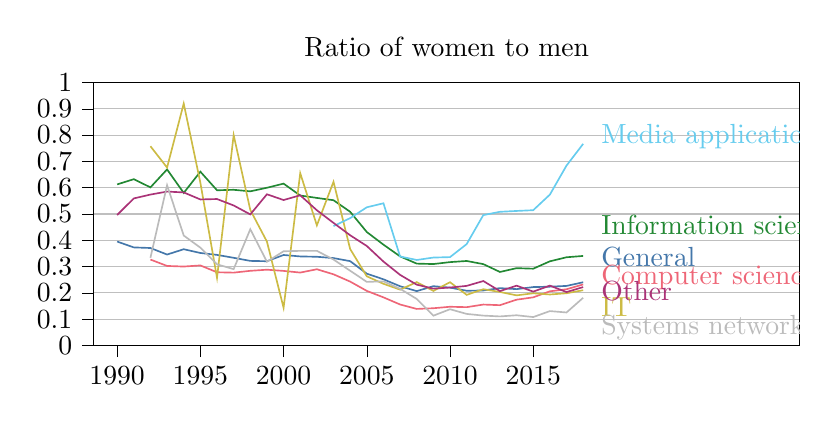
\begin{tikzpicture}

\definecolor{color0}{rgb}{0.266666666666667,0.466666666666667,0.666666666666667}
\definecolor{color1}{rgb}{0.933333333333333,0.4,0.466666666666667}
\definecolor{color2}{rgb}{0.133333333333333,0.533333333333333,0.2}
\definecolor{color3}{rgb}{0.8,0.733333333333333,0.266666666666667}
\definecolor{color4}{rgb}{0.4,0.8,0.933333333333333}
\definecolor{color5}{rgb}{0.666666666666667,0.2,0.466666666666667}

\begin{axis}[
height=140pt,
tick align=outside,
tick pos=left,
title={Ratio of women to men},
unbounded coords=jump,
width=300pt,
x grid style={white!69.0196078431373!black},
xmin=1988.6, xmax=2031,
xtick style={color=black},
xtick={1990,1995,2000,2005,2010,2015},
xticklabels={\(\displaystyle 1990\),\(\displaystyle 1995\),\(\displaystyle 2000\),\(\displaystyle 2005\),\(\displaystyle 2010\),\(\displaystyle 2015\)},
ymajorgrids,
ymin=0, ymax=1,
ytick style={color=black},
ytick={0,0.1,0.2,0.3,0.4,0.5,0.6,0.7,0.8,0.9,1},
yticklabels={\(\displaystyle 0\),\(\displaystyle 0.1\),\(\displaystyle 0.2\),\(\displaystyle 0.3\),\(\displaystyle 0.4\),\(\displaystyle 0.5\),\(\displaystyle 0.6\),\(\displaystyle 0.7\),\(\displaystyle 0.8\),\(\displaystyle 0.9\),\(\displaystyle 1\)}
]
\addplot [semithick, color0]
table {%
1990 0.394967913627625
1991 0.37271773815155
1992 0.370465278625488
1993 0.345574140548706
1994 0.365840792655945
1995 0.351528167724609
1996 0.344272255897522
1997 0.3332200050354
1998 0.321436882019043
1999 0.320170640945435
2000 0.343914747238159
2001 0.338396310806274
2002 0.337104439735413
2003 0.332112669944763
2004 0.320477366447449
2005 0.272923469543457
2006 0.251452445983887
2007 0.225056648254395
2008 0.206436157226562
2009 0.225293636322021
2010 0.219744563102722
2011 0.207880258560181
2012 0.208938837051392
2013 0.217817306518555
2014 0.214048385620117
2015 0.221825838088989
2016 0.223389029502869
2017 0.226261734962463
2018 0.240228176116943
};
\addplot [semithick, color1]
table {%
1990 nan
1991 nan
1992 0.3265465935787
1993 0.302248126561199
1994 0.2999222999223
1995 0.304198473282443
1996 0.278148148148148
1997 0.276795380728979
1998 0.283663704716336
1999 0.287935502447452
2000 0.283360408447436
2001 0.276973281664287
2002 0.289675114815445
2003 0.270382165605096
2004 0.242696416753333
2005 0.207340962985875
2006 0.182779629842511
2007 0.155608214849921
2008 0.13874859708193
2009 0.14136500214623
2010 0.146981988175443
2011 0.145420088439671
2012 0.155357142857143
2013 0.15297619047619
2014 0.173902111967818
2015 0.1828334168516
2016 0.205791482401405
2017 0.2134888957118
2018 0.231927175843694
};
\addplot [semithick, color2]
table {%
1990 0.612352168199737
1991 0.632269348491474
1992 0.601075750784402
1993 0.669402644778842
1994 0.580039920159681
1995 0.66078753076292
1996 0.590057361376673
1997 0.591881116346502
1998 0.586007702182285
1999 0.599660729431722
2000 0.615333035315154
2001 0.570116566584246
2002 0.560919540229885
2003 0.552210724365005
2004 0.508236165093467
2005 0.431290064102564
2006 0.383183709218305
2007 0.338664635694339
2008 0.311026615969582
2009 0.309437854564208
2010 0.316780821917808
2011 0.321109328443731
2012 0.309195912927588
2013 0.279330792037272
2014 0.293806030969845
2015 0.291763791763792
2016 0.319848771266541
2017 0.335242527295507
2018 0.340254305488492
};
\addplot [semithick, color3]
table {%
1990 nan
1991 nan
1992 0.757575757575758
1993 0.676470588235294
1994 0.92
1995 0.619047619047619
1996 0.257142857142857
1997 0.8
1998 0.515151515151515
1999 0.394736842105263
2000 0.142857142857143
2001 0.655172413793103
2002 0.456521739130435
2003 0.622327790973872
2004 0.366598778004073
2005 0.26284751474305
2006 0.234259259259259
2007 0.212081418253447
2008 0.240674501788452
2009 0.20728441349759
2010 0.24040404040404
2011 0.192297111416781
2012 0.213741987179487
2013 0.203204661325564
2014 0.190322580645161
2015 0.198224852071006
2016 0.193636363636364
2017 0.198331193838254
2018 0.209817893903405
};
\addplot [semithick, color4]
table {%
1990 nan
1991 nan
1992 nan
1993 nan
1994 nan
1995 nan
1996 nan
1997 nan
1998 nan
1999 nan
2000 nan
2001 nan
2002 nan
2003 0.453731343283582
2004 0.48406862745098
2005 0.52530779753762
2006 0.540609137055838
2007 0.338213762811127
2008 0.324987963408763
2009 0.334102445777573
2010 0.335807050092764
2011 0.385281385281385
2012 0.495648734177215
2013 0.508133230054222
2014 0.511384845091452
2015 0.514325974635979
2016 0.573572120038722
2017 0.684032802701399
2018 0.766576819407008
};
\addplot [semithick, color5]
table {%
1990 0.496227510156703
1991 0.559025133282559
1992 0.573730862207897
1993 0.585096596136155
1994 0.581833761782348
1995 0.555163283318623
1996 0.556741028128031
1997 0.532289628180039
1998 0.498251748251748
1999 0.57484076433121
2000 0.55296343001261
2001 0.571029529130088
2002 0.514033427940713
2003 0.465948777648428
2004 0.418907007492287
2005 0.37811320754717
2006 0.318900343642612
2007 0.268292682926829
2008 0.230987246102976
2009 0.21584440227704
2010 0.220114689016321
2011 0.226400613967767
2012 0.244788164088769
2013 0.206656101426307
2014 0.227162209100382
2015 0.204568700988749
2016 0.227431770468859
2017 0.202842873607376
2018 0.221844453888653
};
\addplot [semithick, white!73.3333333333333!black]
table {%
1990 nan
1991 nan
1992 0.333333333333333
1993 0.609375
1994 0.417910447761194
1995 0.371794871794872
1996 0.308411214953271
1997 0.290123456790123
1998 0.441913439635535
1999 0.318181818181818
2000 0.358090185676393
2001 0.359615384615385
2002 0.35969387755102
2003 0.326538931920098
2004 0.284086112283664
2005 0.241577335375191
2006 0.243598862019915
2007 0.215324927255092
2008 0.176638176638177
2009 0.113035551504102
2010 0.137533274179237
2011 0.119799139167862
2012 0.113329040566645
2013 0.110236220472441
2014 0.114686951433587
2015 0.107761027359017
2016 0.130511463844797
2017 0.125265392781316
2018 0.181153533712429
};
\draw (axis cs:2018.5,0.300228192859772) node[
  anchor=base west,
  text=color0,
  rotate=0.0
]{General};
\draw (axis cs:2018.5,0.231927175843694) node[
  anchor=base west,
  text=color1,
  rotate=0.0
]{Computer science};
\draw (axis cs:2018.5,0.420254305488492) node[
  anchor=base west,
  text=color2,
  rotate=0.0
]{Information science};
\draw (axis cs:2018.5,0.109817893903405) node[
  anchor=base west,
  text=color3,
  rotate=0.0
]{IT};
\draw (axis cs:2018.5,0.766576819407008) node[
  anchor=base west,
  text=color4,
  rotate=0.0
]{Media applications};
\draw (axis cs:2018.5,0.171844453888653) node[
  anchor=base west,
  text=color5,
  rotate=0.0
]{Other};
\draw (axis cs:2018.5,0.0411535337124289) node[
  anchor=base west,
  text=white!73.3333333333333!black,
  rotate=0.0
]{Systems network};
\end{axis}

\end{tikzpicture}

\vspace{0.1cm}
\begin{tikzpicture}
% This file was created by tikzplotlib v0.9.2.
\definecolor{color0}{rgb}{0.266666666666667,0.466666666666667,0.666666666666667}
\definecolor{color1}{rgb}{0.933333333333333,0.4,0.466666666666667}
\definecolor{color2}{rgb}{0.133333333333333,0.533333333333333,0.2}
\definecolor{color3}{rgb}{0.8,0.733333333333333,0.266666666666667}
\definecolor{color4}{rgb}{0.4,0.8,0.933333333333333}
\definecolor{color5}{rgb}{0.666666666666667,0.2,0.466666666666667}

\begin{groupplot}[group style={group size=2 by 1, group name=my plots, horizontal sep=0.8cm}]
\nextgroupplot[
height=90pt, width=160pt,
legend style={at={(2.02, 0.5)},anchor=west,},
reverse legend,
tick align=outside,
tick pos=left,
x grid style={white!69.0196078431373!black},
xlabel={Women},
xmin=1988.6, xmax=2019.4,
xtick style={color=black},
xtick={1990,2000,2010},
xticklabels={\(\displaystyle 1990\),\(\displaystyle 2000\),\(\displaystyle 2010\)},
ymajorgrids,
ymin=0, ymax=17.94555,
ytick style={color=black}
]
\path [draw=color0, fill=color0]
(axis cs:1990,6.028)
--(axis cs:1990,0)
--(axis cs:1991,0)
--(axis cs:1992,0)
--(axis cs:1993,0)
--(axis cs:1994,0)
--(axis cs:1995,0)
--(axis cs:1996,0)
--(axis cs:1997,0)
--(axis cs:1998,0)
--(axis cs:1999,0)
--(axis cs:2000,0)
--(axis cs:2001,0)
--(axis cs:2002,0)
--(axis cs:2003,0)
--(axis cs:2004,0)
--(axis cs:2005,0)
--(axis cs:2006,0)
--(axis cs:2007,0)
--(axis cs:2008,0)
--(axis cs:2009,0)
--(axis cs:2010,0)
--(axis cs:2011,0)
--(axis cs:2012,0)
--(axis cs:2013,0)
--(axis cs:2014,0)
--(axis cs:2015,0)
--(axis cs:2016,0)
--(axis cs:2017,0)
--(axis cs:2018,0)
--(axis cs:2018,6.527)
--(axis cs:2018,6.527)
--(axis cs:2017,5.483)
--(axis cs:2016,4.85)
--(axis cs:2015,4.291)
--(axis cs:2014,3.736)
--(axis cs:2013,3.423)
--(axis cs:2012,3.048)
--(axis cs:2011,2.944)
--(axis cs:2010,2.976)
--(axis cs:2009,3.203)
--(axis cs:2008,2.489)
--(axis cs:2007,3.679)
--(axis cs:2006,4.501)
--(axis cs:2005,5.566)
--(axis cs:2004,6.955)
--(axis cs:2003,6.439)
--(axis cs:2002,6.913)
--(axis cs:2001,6.461)
--(axis cs:2000,5.612)
--(axis cs:1999,4.354)
--(axis cs:1998,4.152)
--(axis cs:1997,3.922)
--(axis cs:1996,3.955)
--(axis cs:1995,4.083)
--(axis cs:1994,4.164)
--(axis cs:1993,4.15)
--(axis cs:1992,4.34)
--(axis cs:1991,5.328)
--(axis cs:1990,6.028)
--cycle;

\path [draw=color1, fill=color1]
(axis cs:1990,6.028)
--(axis cs:1990,6.028)
--(axis cs:1991,5.328)
--(axis cs:1992,4.34)
--(axis cs:1993,4.15)
--(axis cs:1994,4.164)
--(axis cs:1995,4.083)
--(axis cs:1996,3.955)
--(axis cs:1997,3.922)
--(axis cs:1998,4.152)
--(axis cs:1999,4.354)
--(axis cs:2000,5.612)
--(axis cs:2001,6.461)
--(axis cs:2002,6.913)
--(axis cs:2003,6.439)
--(axis cs:2004,6.955)
--(axis cs:2005,5.566)
--(axis cs:2006,4.501)
--(axis cs:2007,3.679)
--(axis cs:2008,2.489)
--(axis cs:2009,3.203)
--(axis cs:2010,2.976)
--(axis cs:2011,2.944)
--(axis cs:2012,3.048)
--(axis cs:2013,3.423)
--(axis cs:2014,3.736)
--(axis cs:2015,4.291)
--(axis cs:2016,4.85)
--(axis cs:2017,5.483)
--(axis cs:2018,6.527)
--(axis cs:2018,11.75)
--(axis cs:2018,11.75)
--(axis cs:2017,9.655)
--(axis cs:2016,8.247)
--(axis cs:2015,6.845)
--(axis cs:2014,5.811)
--(axis cs:2013,4.965)
--(axis cs:2012,4.44)
--(axis cs:2011,4.095)
--(axis cs:2010,4.045)
--(axis cs:2009,4.191)
--(axis cs:2008,3.478)
--(axis cs:2007,4.861)
--(axis cs:2006,6.091)
--(axis cs:2005,7.577)
--(axis cs:2004,9.522)
--(axis cs:2003,8.986)
--(axis cs:2002,8.616)
--(axis cs:2001,7.819)
--(axis cs:2000,6.833)
--(axis cs:1999,5.354)
--(axis cs:1998,4.982)
--(axis cs:1997,4.689)
--(axis cs:1996,4.706)
--(axis cs:1995,4.88)
--(axis cs:1994,4.936)
--(axis cs:1993,4.876)
--(axis cs:1992,5.174)
--(axis cs:1991,5.328)
--(axis cs:1990,6.028)
--cycle;

\path [draw=color2, fill=color2]
(axis cs:1990,7.426)
--(axis cs:1990,6.028)
--(axis cs:1991,5.328)
--(axis cs:1992,5.174)
--(axis cs:1993,4.876)
--(axis cs:1994,4.936)
--(axis cs:1995,4.88)
--(axis cs:1996,4.706)
--(axis cs:1997,4.689)
--(axis cs:1998,4.982)
--(axis cs:1999,5.354)
--(axis cs:2000,6.833)
--(axis cs:2001,7.819)
--(axis cs:2002,8.616)
--(axis cs:2003,8.986)
--(axis cs:2004,9.522)
--(axis cs:2005,7.577)
--(axis cs:2006,6.091)
--(axis cs:2007,4.861)
--(axis cs:2008,3.478)
--(axis cs:2009,4.191)
--(axis cs:2010,4.045)
--(axis cs:2011,4.095)
--(axis cs:2012,4.44)
--(axis cs:2013,4.965)
--(axis cs:2014,5.811)
--(axis cs:2015,6.845)
--(axis cs:2016,8.247)
--(axis cs:2017,9.655)
--(axis cs:2018,11.75)
--(axis cs:2018,13.864)
--(axis cs:2018,13.864)
--(axis cs:2017,11.528)
--(axis cs:2016,9.939)
--(axis cs:2015,8.347)
--(axis cs:2014,7.253)
--(axis cs:2013,6.284)
--(axis cs:2012,5.832)
--(axis cs:2011,5.496)
--(axis cs:2010,5.34)
--(axis cs:2009,5.391)
--(axis cs:2008,4.705)
--(axis cs:2007,6.195)
--(axis cs:2006,7.841)
--(axis cs:2005,9.73)
--(axis cs:2004,12.268)
--(axis cs:2003,13.095)
--(axis cs:2002,12.276)
--(axis cs:2001,11.047)
--(axis cs:2000,9.586)
--(axis cs:1999,7.475)
--(axis cs:1998,6.808)
--(axis cs:1997,6.322)
--(axis cs:1996,6.249)
--(axis cs:1995,6.491)
--(axis cs:1994,6.389)
--(axis cs:1993,6.344)
--(axis cs:1992,6.515)
--(axis cs:1991,6.774)
--(axis cs:1990,7.426)
--cycle;

\path [draw=color3, fill=color3]
(axis cs:1990,7.426)
--(axis cs:1990,7.426)
--(axis cs:1991,6.774)
--(axis cs:1992,6.515)
--(axis cs:1993,6.344)
--(axis cs:1994,6.389)
--(axis cs:1995,6.491)
--(axis cs:1996,6.249)
--(axis cs:1997,6.322)
--(axis cs:1998,6.808)
--(axis cs:1999,7.475)
--(axis cs:2000,9.586)
--(axis cs:2001,11.047)
--(axis cs:2002,12.276)
--(axis cs:2003,13.095)
--(axis cs:2004,12.268)
--(axis cs:2005,9.73)
--(axis cs:2006,7.841)
--(axis cs:2007,6.195)
--(axis cs:2008,4.705)
--(axis cs:2009,5.391)
--(axis cs:2010,5.34)
--(axis cs:2011,5.496)
--(axis cs:2012,5.832)
--(axis cs:2013,6.284)
--(axis cs:2014,7.253)
--(axis cs:2015,8.347)
--(axis cs:2016,9.939)
--(axis cs:2017,11.528)
--(axis cs:2018,13.864)
--(axis cs:2018,14.924)
--(axis cs:2018,14.924)
--(axis cs:2017,12.455)
--(axis cs:2016,10.791)
--(axis cs:2015,9.419)
--(axis cs:2014,8.315)
--(axis cs:2013,7.4)
--(axis cs:2012,6.899)
--(axis cs:2011,6.195)
--(axis cs:2010,5.935)
--(axis cs:2009,5.778)
--(axis cs:2008,5.647)
--(axis cs:2007,6.518)
--(axis cs:2006,8.094)
--(axis cs:2005,10.042)
--(axis cs:2004,12.448)
--(axis cs:2003,13.357)
--(axis cs:2002,12.297)
--(axis cs:2001,11.066)
--(axis cs:2000,9.591)
--(axis cs:1999,7.49)
--(axis cs:1998,6.825)
--(axis cs:1997,6.338)
--(axis cs:1996,6.258)
--(axis cs:1995,6.504)
--(axis cs:1994,6.412)
--(axis cs:1993,6.367)
--(axis cs:1992,6.54)
--(axis cs:1991,6.774)
--(axis cs:1990,7.426)
--cycle;

\path [draw=color4, fill=color4]
(axis cs:1990,7.426)
--(axis cs:1990,7.426)
--(axis cs:1991,6.774)
--(axis cs:1992,6.54)
--(axis cs:1993,6.367)
--(axis cs:1994,6.412)
--(axis cs:1995,6.504)
--(axis cs:1996,6.258)
--(axis cs:1997,6.338)
--(axis cs:1998,6.825)
--(axis cs:1999,7.49)
--(axis cs:2000,9.591)
--(axis cs:2001,11.066)
--(axis cs:2002,12.297)
--(axis cs:2003,13.357)
--(axis cs:2004,12.448)
--(axis cs:2005,10.042)
--(axis cs:2006,8.094)
--(axis cs:2007,6.518)
--(axis cs:2008,5.647)
--(axis cs:2009,5.778)
--(axis cs:2010,5.935)
--(axis cs:2011,6.195)
--(axis cs:2012,6.899)
--(axis cs:2013,7.4)
--(axis cs:2014,8.315)
--(axis cs:2015,9.419)
--(axis cs:2016,10.791)
--(axis cs:2017,12.455)
--(axis cs:2018,14.924)
--(axis cs:2018,16.346)
--(axis cs:2018,16.346)
--(axis cs:2017,13.873)
--(axis cs:2016,11.976)
--(axis cs:2015,10.514)
--(axis cs:2014,9.685)
--(axis cs:2013,8.712)
--(axis cs:2012,8.152)
--(axis cs:2011,7.174)
--(axis cs:2010,6.84)
--(axis cs:2009,6.502)
--(axis cs:2008,6.322)
--(axis cs:2007,6.98)
--(axis cs:2006,8.52)
--(axis cs:2005,10.426)
--(axis cs:2004,12.843)
--(axis cs:2003,13.661)
--(axis cs:2002,12.297)
--(axis cs:2001,11.066)
--(axis cs:2000,9.591)
--(axis cs:1999,7.49)
--(axis cs:1998,6.825)
--(axis cs:1997,6.338)
--(axis cs:1996,6.258)
--(axis cs:1995,6.504)
--(axis cs:1994,6.412)
--(axis cs:1993,6.367)
--(axis cs:1992,6.54)
--(axis cs:1991,6.774)
--(axis cs:1990,7.426)
--cycle;

\path [draw=color5, fill=color5]
(axis cs:1990,8.281)
--(axis cs:1990,7.426)
--(axis cs:1991,6.774)
--(axis cs:1992,6.54)
--(axis cs:1993,6.367)
--(axis cs:1994,6.412)
--(axis cs:1995,6.504)
--(axis cs:1996,6.258)
--(axis cs:1997,6.338)
--(axis cs:1998,6.825)
--(axis cs:1999,7.49)
--(axis cs:2000,9.591)
--(axis cs:2001,11.066)
--(axis cs:2002,12.297)
--(axis cs:2003,13.661)
--(axis cs:2004,12.843)
--(axis cs:2005,10.426)
--(axis cs:2006,8.52)
--(axis cs:2007,6.98)
--(axis cs:2008,6.322)
--(axis cs:2009,6.502)
--(axis cs:2010,6.84)
--(axis cs:2011,7.174)
--(axis cs:2012,8.152)
--(axis cs:2013,8.712)
--(axis cs:2014,9.685)
--(axis cs:2015,10.514)
--(axis cs:2016,11.976)
--(axis cs:2017,13.873)
--(axis cs:2018,16.346)
--(axis cs:2018,16.868)
--(axis cs:2018,16.868)
--(axis cs:2017,14.401)
--(axis cs:2016,12.626)
--(axis cs:2015,11.114)
--(axis cs:2014,10.339)
--(axis cs:2013,9.364)
--(axis cs:2012,8.88)
--(axis cs:2011,7.764)
--(axis cs:2010,7.339)
--(axis cs:2009,6.957)
--(axis cs:2008,6.811)
--(axis cs:2007,7.651)
--(axis cs:2006,9.448)
--(axis cs:2005,11.929)
--(axis cs:2004,14.744)
--(axis cs:2003,15.262)
--(axis cs:2002,13.927)
--(axis cs:2001,12.497)
--(axis cs:2000,10.468)
--(axis cs:1999,8.212)
--(axis cs:1998,7.395)
--(axis cs:1997,6.882)
--(axis cs:1996,6.832)
--(axis cs:1995,7.133)
--(axis cs:1994,7.091)
--(axis cs:1993,7.003)
--(axis cs:1992,7.252)
--(axis cs:1991,7.508)
--(axis cs:1990,8.281)
--cycle;

\path [draw=white!73.3333333333333!black, fill=white!73.3333333333333!black]
(axis cs:1990,8.281)
--(axis cs:1990,8.281)
--(axis cs:1991,7.508)
--(axis cs:1992,7.252)
--(axis cs:1993,7.003)
--(axis cs:1994,7.091)
--(axis cs:1995,7.133)
--(axis cs:1996,6.832)
--(axis cs:1997,6.882)
--(axis cs:1998,7.395)
--(axis cs:1999,8.212)
--(axis cs:2000,10.468)
--(axis cs:2001,12.497)
--(axis cs:2002,13.927)
--(axis cs:2003,15.262)
--(axis cs:2004,14.744)
--(axis cs:2005,11.929)
--(axis cs:2006,9.448)
--(axis cs:2007,7.651)
--(axis cs:2008,6.811)
--(axis cs:2009,6.957)
--(axis cs:2010,7.339)
--(axis cs:2011,7.764)
--(axis cs:2012,8.88)
--(axis cs:2013,9.364)
--(axis cs:2014,10.339)
--(axis cs:2015,11.114)
--(axis cs:2016,12.626)
--(axis cs:2017,14.401)
--(axis cs:2018,16.868)
--(axis cs:2018,17.091)
--(axis cs:2018,17.091)
--(axis cs:2017,14.578)
--(axis cs:2016,12.848)
--(axis cs:2015,11.307)
--(axis cs:2014,10.535)
--(axis cs:2013,9.546)
--(axis cs:2012,9.056)
--(axis cs:2011,7.931)
--(axis cs:2010,7.494)
--(axis cs:2009,7.081)
--(axis cs:2008,7.059)
--(axis cs:2007,8.095)
--(axis cs:2006,10.133)
--(axis cs:2005,12.56)
--(axis cs:2004,15.417)
--(axis cs:2003,16.063)
--(axis cs:2002,14.491)
--(axis cs:2001,12.871)
--(axis cs:2000,10.738)
--(axis cs:1999,8.408)
--(axis cs:1998,7.589)
--(axis cs:1997,6.976)
--(axis cs:1996,6.865)
--(axis cs:1995,7.162)
--(axis cs:1994,7.119)
--(axis cs:1993,7.042)
--(axis cs:1992,7.278)
--(axis cs:1991,7.508)
--(axis cs:1990,8.281)
--cycle;

\addplot [semithick, color0]
table {%
1990 6.02799987792969
1991 5.32800006866455
1992 4.34000015258789
1993 4.15000009536743
1994 4.16400003433228
1995 4.08300018310547
1996 3.95499992370605
1997 3.92199993133545
1998 4.15199995040894
1999 4.35400009155273
2000 5.61199998855591
2001 6.46099996566772
2002 6.91300010681152
2003 6.43900012969971
2004 6.95499992370605
2005 5.56599998474121
2006 4.50099992752075
2007 3.67899990081787
2008 2.48900008201599
2009 3.20300006866455
2010 2.9760000705719
2011 2.94400000572205
2012 3.04800009727478
2013 3.42300009727478
2014 3.73600006103516
2016 4.84999990463257
2017 5.48299980163574
2018 6.52699995040894
};
\addplot [semithick, color1]
table {%
1990 6.02799987792969
1991 5.32800006866455
1992 5.17399978637695
1993 4.87599992752075
1994 4.93599987030029
1995 4.88000011444092
1996 4.70599985122681
1997 4.68900012969971
1998 4.98199987411499
1999 5.35400009155273
2000 6.83300018310547
2001 7.81899976730347
2002 8.61600017547607
2003 8.98600006103516
2004 9.52200031280518
2005 7.5770001411438
2006 6.09100008010864
2007 4.86100006103516
2008 3.4779999256134
2009 4.19099998474121
2010 4.04500007629395
2011 4.09499979019165
2012 4.44000005722046
2013 4.96500015258789
2014 5.81099987030029
2015 6.84499979019165
2017 9.65499973297119
2018 11.75
};
\addplot [semithick, color2]
table {%
1990 7.42600011825562
1991 6.77400016784668
1992 6.5149998664856
1993 6.3439998626709
1994 6.38899993896484
1995 6.49100017547607
1996 6.24900007247925
1997 6.32200002670288
1998 6.80800008773804
1999 7.47499990463257
2000 9.58600044250488
2001 11.0469999313354
2002 12.2760000228882
2003 13.0950002670288
2004 12.2679996490479
2005 9.72999954223633
2006 7.84100008010864
2007 6.19500017166138
2008 4.70499992370605
2009 5.39099979400635
2010 5.34000015258789
2011 5.49599981307983
2012 5.83199977874756
2013 6.28399991989136
2014 7.25299978256226
2015 8.34700012207031
2017 11.5279998779297
2018 13.8640003204346
};
\addplot [semithick, color3]
table {%
1990 7.42600011825562
1991 6.77400016784668
1992 6.53999996185303
1993 6.36700010299683
1994 6.41200017929077
1995 6.50400018692017
1996 6.25799989700317
1997 6.33799982070923
1998 6.82499980926514
1999 7.48999977111816
2000 9.59099960327148
2001 11.0659999847412
2002 12.2969999313354
2003 13.3570003509521
2004 12.4479999542236
2005 10.0419998168945
2006 8.0939998626709
2007 6.51800012588501
2008 5.64699983596802
2009 5.77799987792969
2010 5.93499994277954
2011 6.19500017166138
2012 6.89900016784668
2013 7.40000009536743
2014 8.3149995803833
2015 9.41899967193604
2016 10.7910003662109
2017 12.4549999237061
2018 14.923999786377
};
\addplot [semithick, color4]
table {%
1990 7.42600011825562
1991 6.77400016784668
1992 6.53999996185303
1993 6.36700010299683
1994 6.41200017929077
1995 6.50400018692017
1996 6.25799989700317
1997 6.33799982070923
1998 6.82499980926514
1999 7.48999977111816
2000 9.59099960327148
2001 11.0659999847412
2002 12.2969999313354
2003 13.66100025177
2004 12.8430004119873
2005 10.4259996414185
2006 8.52000045776367
2007 6.98000001907349
2008 6.32200002670288
2009 6.5019998550415
2011 7.17399978637695
2012 8.15200042724609
2013 8.71199989318848
2014 9.6850004196167
2015 10.5139999389648
2016 11.9759998321533
2017 13.8730001449585
2018 16.3460006713867
};
\addplot [semithick, color5]
table {%
1990 8.2810001373291
1991 7.50799989700317
1992 7.2519998550415
1993 7.00299978256226
1994 7.09100008010864
1995 7.13299989700317
1996 6.83199977874756
1997 6.88199996948242
1998 7.39499998092651
1999 8.21199989318848
2000 10.4680004119873
2001 12.4969997406006
2002 13.9270000457764
2003 15.2620000839233
2004 14.7440004348755
2005 11.9289999008179
2006 9.44799995422363
2007 7.65100002288818
2008 6.81099987030029
2009 6.95699977874756
2010 7.33900022506714
2011 7.76399993896484
2012 8.88000011444092
2013 9.36400032043457
2014 10.33899974823
2015 11.1140003204346
2016 12.6260004043579
2017 14.4010000228882
2018 16.8680000305176
};
\addplot [semithick, white!73.3333333333333!black]
table {%
1990 8.2810001373291
1991 7.50799989700317
1993 7.04199981689453
1994 7.11899995803833
1995 7.16200017929077
1996 6.86499977111816
1997 6.97599983215332
1998 7.58900022506714
1999 8.40799999237061
2000 10.7379999160767
2001 12.871000289917
2002 14.4910001754761
2003 16.0629997253418
2004 15.4169998168945
2005 12.5600004196167
2006 10.1330003738403
2007 8.09500026702881
2008 7.05900001525879
2009 7.08099985122681
2010 7.49399995803833
2011 7.93100023269653
2012 9.05599975585938
2013 9.54599952697754
2014 10.5349998474121
2015 11.3070001602173
2016 12.8479995727539
2017 14.5780000686646
2018 17.0909996032715
};

\nextgroupplot[
height=90pt, width=160pt,
legend style={at={(2.02, 0.5)},anchor=west,},
reverse legend,
tick align=outside,
tick pos=left,
x grid style={white!69.0196078431373!black},
xlabel={Men},
xmin=1988.6, xmax=2019.4,
xtick style={color=black},
xtick={1990,2000,2010},
xticklabels={\(\displaystyle 1990\),\(\displaystyle 2000\),\(\displaystyle 2010\)},
ymajorgrids,
ymin=0, ymax=69.7137,
ytick style={color=black}
]
\path [draw=color0, fill=color0]
(axis cs:1990,15.262)
--(axis cs:1990,0)
--(axis cs:1991,0)
--(axis cs:1992,0)
--(axis cs:1993,0)
--(axis cs:1994,0)
--(axis cs:1995,0)
--(axis cs:1996,0)
--(axis cs:1997,0)
--(axis cs:1998,0)
--(axis cs:1999,0)
--(axis cs:2000,0)
--(axis cs:2001,0)
--(axis cs:2002,0)
--(axis cs:2003,0)
--(axis cs:2004,0)
--(axis cs:2005,0)
--(axis cs:2006,0)
--(axis cs:2007,0)
--(axis cs:2008,0)
--(axis cs:2009,0)
--(axis cs:2010,0)
--(axis cs:2011,0)
--(axis cs:2012,0)
--(axis cs:2013,0)
--(axis cs:2014,0)
--(axis cs:2015,0)
--(axis cs:2016,0)
--(axis cs:2017,0)
--(axis cs:2018,0)
--(axis cs:2018,27.17)
--(axis cs:2018,27.17)
--(axis cs:2017,24.233)
--(axis cs:2016,21.711)
--(axis cs:2015,19.344)
--(axis cs:2014,17.454)
--(axis cs:2013,15.715)
--(axis cs:2012,14.588)
--(axis cs:2011,14.162)
--(axis cs:2010,13.543)
--(axis cs:2009,14.217)
--(axis cs:2008,12.057)
--(axis cs:2007,16.347)
--(axis cs:2006,17.9)
--(axis cs:2005,20.394)
--(axis cs:2004,21.702)
--(axis cs:2003,19.388)
--(axis cs:2002,20.507)
--(axis cs:2001,19.093)
--(axis cs:2000,16.318)
--(axis cs:1999,13.599)
--(axis cs:1998,12.917)
--(axis cs:1997,11.77)
--(axis cs:1996,11.488)
--(axis cs:1995,11.615)
--(axis cs:1994,11.382)
--(axis cs:1993,12.009)
--(axis cs:1992,11.715)
--(axis cs:1991,14.295)
--(axis cs:1990,15.262)
--cycle;

\path [draw=color1, fill=color1]
(axis cs:1990,15.262)
--(axis cs:1990,15.262)
--(axis cs:1991,14.295)
--(axis cs:1992,11.715)
--(axis cs:1993,12.009)
--(axis cs:1994,11.382)
--(axis cs:1995,11.615)
--(axis cs:1996,11.488)
--(axis cs:1997,11.77)
--(axis cs:1998,12.917)
--(axis cs:1999,13.599)
--(axis cs:2000,16.318)
--(axis cs:2001,19.093)
--(axis cs:2002,20.507)
--(axis cs:2003,19.388)
--(axis cs:2004,21.702)
--(axis cs:2005,20.394)
--(axis cs:2006,17.9)
--(axis cs:2007,16.347)
--(axis cs:2008,12.057)
--(axis cs:2009,14.217)
--(axis cs:2010,13.543)
--(axis cs:2011,14.162)
--(axis cs:2012,14.588)
--(axis cs:2013,15.715)
--(axis cs:2014,17.454)
--(axis cs:2015,19.344)
--(axis cs:2016,21.711)
--(axis cs:2017,24.233)
--(axis cs:2018,27.17)
--(axis cs:2018,49.69)
--(axis cs:2018,49.69)
--(axis cs:2017,43.775)
--(axis cs:2016,38.218)
--(axis cs:2015,33.313)
--(axis cs:2014,29.386)
--(axis cs:2013,25.795)
--(axis cs:2012,23.548)
--(axis cs:2011,22.077)
--(axis cs:2010,20.816)
--(axis cs:2009,21.206)
--(axis cs:2008,19.185)
--(axis cs:2007,23.943)
--(axis cs:2006,26.599)
--(axis cs:2005,30.093)
--(axis cs:2004,32.279)
--(axis cs:2003,28.808)
--(axis cs:2002,26.386)
--(axis cs:2001,23.996)
--(axis cs:2000,20.627)
--(axis cs:1999,17.072)
--(axis cs:1998,15.843)
--(axis cs:1997,14.541)
--(axis cs:1996,14.188)
--(axis cs:1995,14.235)
--(axis cs:1994,13.956)
--(axis cs:1993,14.411)
--(axis cs:1992,14.269)
--(axis cs:1991,14.295)
--(axis cs:1990,15.262)
--cycle;

\path [draw=color2, fill=color2]
(axis cs:1990,17.545)
--(axis cs:1990,15.262)
--(axis cs:1991,14.295)
--(axis cs:1992,14.269)
--(axis cs:1993,14.411)
--(axis cs:1994,13.956)
--(axis cs:1995,14.235)
--(axis cs:1996,14.188)
--(axis cs:1997,14.541)
--(axis cs:1998,15.843)
--(axis cs:1999,17.072)
--(axis cs:2000,20.627)
--(axis cs:2001,23.996)
--(axis cs:2002,26.386)
--(axis cs:2003,28.808)
--(axis cs:2004,32.279)
--(axis cs:2005,30.093)
--(axis cs:2006,26.599)
--(axis cs:2007,23.943)
--(axis cs:2008,19.185)
--(axis cs:2009,21.206)
--(axis cs:2010,20.816)
--(axis cs:2011,22.077)
--(axis cs:2012,23.548)
--(axis cs:2013,25.795)
--(axis cs:2014,29.386)
--(axis cs:2015,33.313)
--(axis cs:2016,38.218)
--(axis cs:2017,43.775)
--(axis cs:2018,49.69)
--(axis cs:2018,55.903)
--(axis cs:2018,55.903)
--(axis cs:2017,49.362)
--(axis cs:2016,43.508)
--(axis cs:2015,38.461)
--(axis cs:2014,34.294)
--(axis cs:2013,30.517)
--(axis cs:2012,28.05)
--(axis cs:2011,26.44)
--(axis cs:2010,24.904)
--(axis cs:2009,25.084)
--(axis cs:2008,23.13)
--(axis cs:2007,27.882)
--(axis cs:2006,31.166)
--(axis cs:2005,35.085)
--(axis cs:2004,37.682)
--(axis cs:2003,36.249)
--(axis cs:2002,32.911)
--(axis cs:2001,29.658)
--(axis cs:2000,25.101)
--(axis cs:1999,20.609)
--(axis cs:1998,18.959)
--(axis cs:1997,17.3)
--(axis cs:1996,16.803)
--(axis cs:1995,16.673)
--(axis cs:1994,16.461)
--(axis cs:1993,16.604)
--(axis cs:1992,16.5)
--(axis cs:1991,16.582)
--(axis cs:1990,17.545)
--cycle;

\path [draw=color3, fill=color3]
(axis cs:1990,17.545)
--(axis cs:1990,17.545)
--(axis cs:1991,16.582)
--(axis cs:1992,16.5)
--(axis cs:1993,16.604)
--(axis cs:1994,16.461)
--(axis cs:1995,16.673)
--(axis cs:1996,16.803)
--(axis cs:1997,17.3)
--(axis cs:1998,18.959)
--(axis cs:1999,20.609)
--(axis cs:2000,25.101)
--(axis cs:2001,29.658)
--(axis cs:2002,32.911)
--(axis cs:2003,36.249)
--(axis cs:2004,37.682)
--(axis cs:2005,35.085)
--(axis cs:2006,31.166)
--(axis cs:2007,27.882)
--(axis cs:2008,23.13)
--(axis cs:2009,25.084)
--(axis cs:2010,24.904)
--(axis cs:2011,26.44)
--(axis cs:2012,28.05)
--(axis cs:2013,30.517)
--(axis cs:2014,34.294)
--(axis cs:2015,38.461)
--(axis cs:2016,43.508)
--(axis cs:2017,49.362)
--(axis cs:2018,55.903)
--(axis cs:2018,60.955)
--(axis cs:2018,60.955)
--(axis cs:2017,54.036)
--(axis cs:2016,47.908)
--(axis cs:2015,43.869)
--(axis cs:2014,39.874)
--(axis cs:2013,36.009)
--(axis cs:2012,33.042)
--(axis cs:2011,30.075)
--(axis cs:2010,27.379)
--(axis cs:2009,26.951)
--(axis cs:2008,27.044)
--(axis cs:2007,29.405)
--(axis cs:2006,32.246)
--(axis cs:2005,36.272)
--(axis cs:2004,38.173)
--(axis cs:2003,36.67)
--(axis cs:2002,32.957)
--(axis cs:2001,29.687)
--(axis cs:2000,25.136)
--(axis cs:1999,20.647)
--(axis cs:1998,18.992)
--(axis cs:1997,17.32)
--(axis cs:1996,16.838)
--(axis cs:1995,16.694)
--(axis cs:1994,16.486)
--(axis cs:1993,16.638)
--(axis cs:1992,16.533)
--(axis cs:1991,16.582)
--(axis cs:1990,17.545)
--cycle;

\path [draw=color4, fill=color4]
(axis cs:1990,17.545)
--(axis cs:1990,17.545)
--(axis cs:1991,16.582)
--(axis cs:1992,16.533)
--(axis cs:1993,16.638)
--(axis cs:1994,16.486)
--(axis cs:1995,16.694)
--(axis cs:1996,16.838)
--(axis cs:1997,17.32)
--(axis cs:1998,18.992)
--(axis cs:1999,20.647)
--(axis cs:2000,25.136)
--(axis cs:2001,29.687)
--(axis cs:2002,32.957)
--(axis cs:2003,36.67)
--(axis cs:2004,38.173)
--(axis cs:2005,36.272)
--(axis cs:2006,32.246)
--(axis cs:2007,29.405)
--(axis cs:2008,27.044)
--(axis cs:2009,26.951)
--(axis cs:2010,27.379)
--(axis cs:2011,30.075)
--(axis cs:2012,33.042)
--(axis cs:2013,36.009)
--(axis cs:2014,39.874)
--(axis cs:2015,43.869)
--(axis cs:2016,47.908)
--(axis cs:2017,54.036)
--(axis cs:2018,60.955)
--(axis cs:2018,62.81)
--(axis cs:2018,62.81)
--(axis cs:2017,56.109)
--(axis cs:2016,49.974)
--(axis cs:2015,45.998)
--(axis cs:2014,42.553)
--(axis cs:2013,38.591)
--(axis cs:2012,35.57)
--(axis cs:2011,32.616)
--(axis cs:2010,30.074)
--(axis cs:2009,29.118)
--(axis cs:2008,29.121)
--(axis cs:2007,30.771)
--(axis cs:2006,33.034)
--(axis cs:2005,37.003)
--(axis cs:2004,38.989)
--(axis cs:2003,37.34)
--(axis cs:2002,32.957)
--(axis cs:2001,29.687)
--(axis cs:2000,25.136)
--(axis cs:1999,20.647)
--(axis cs:1998,18.992)
--(axis cs:1997,17.32)
--(axis cs:1996,16.838)
--(axis cs:1995,16.694)
--(axis cs:1994,16.486)
--(axis cs:1993,16.638)
--(axis cs:1992,16.533)
--(axis cs:1991,16.582)
--(axis cs:1990,17.545)
--cycle;

\path [draw=color5, fill=color5]
(axis cs:1990,19.268)
--(axis cs:1990,17.545)
--(axis cs:1991,16.582)
--(axis cs:1992,16.533)
--(axis cs:1993,16.638)
--(axis cs:1994,16.486)
--(axis cs:1995,16.694)
--(axis cs:1996,16.838)
--(axis cs:1997,17.32)
--(axis cs:1998,18.992)
--(axis cs:1999,20.647)
--(axis cs:2000,25.136)
--(axis cs:2001,29.687)
--(axis cs:2002,32.957)
--(axis cs:2003,37.34)
--(axis cs:2004,38.989)
--(axis cs:2005,37.003)
--(axis cs:2006,33.034)
--(axis cs:2007,30.771)
--(axis cs:2008,29.121)
--(axis cs:2009,29.118)
--(axis cs:2010,30.074)
--(axis cs:2011,32.616)
--(axis cs:2012,35.57)
--(axis cs:2013,38.591)
--(axis cs:2014,42.553)
--(axis cs:2015,45.998)
--(axis cs:2016,49.974)
--(axis cs:2017,56.109)
--(axis cs:2018,62.81)
--(axis cs:2018,65.163)
--(axis cs:2018,65.163)
--(axis cs:2017,58.712)
--(axis cs:2016,52.832)
--(axis cs:2015,48.931)
--(axis cs:2014,45.432)
--(axis cs:2013,41.746)
--(axis cs:2012,38.544)
--(axis cs:2011,35.222)
--(axis cs:2010,32.341)
--(axis cs:2009,31.226)
--(axis cs:2008,31.238)
--(axis cs:2007,33.272)
--(axis cs:2006,35.944)
--(axis cs:2005,40.978)
--(axis cs:2004,43.527)
--(axis cs:2003,40.776)
--(axis cs:2002,36.128)
--(axis cs:2001,32.193)
--(axis cs:2000,26.722)
--(axis cs:1999,21.903)
--(axis cs:1998,20.136)
--(axis cs:1997,18.342)
--(axis cs:1996,17.869)
--(axis cs:1995,17.827)
--(axis cs:1994,17.653)
--(axis cs:1993,17.725)
--(axis cs:1992,17.774)
--(axis cs:1991,17.895)
--(axis cs:1990,19.268)
--cycle;

\path [draw=white!73.3333333333333!black, fill=white!73.3333333333333!black]
(axis cs:1990,19.268)
--(axis cs:1990,19.268)
--(axis cs:1991,17.895)
--(axis cs:1992,17.774)
--(axis cs:1993,17.725)
--(axis cs:1994,17.653)
--(axis cs:1995,17.827)
--(axis cs:1996,17.869)
--(axis cs:1997,18.342)
--(axis cs:1998,20.136)
--(axis cs:1999,21.903)
--(axis cs:2000,26.722)
--(axis cs:2001,32.193)
--(axis cs:2002,36.128)
--(axis cs:2003,40.776)
--(axis cs:2004,43.527)
--(axis cs:2005,40.978)
--(axis cs:2006,35.944)
--(axis cs:2007,33.272)
--(axis cs:2008,31.238)
--(axis cs:2009,31.226)
--(axis cs:2010,32.341)
--(axis cs:2011,35.222)
--(axis cs:2012,38.544)
--(axis cs:2013,41.746)
--(axis cs:2014,45.432)
--(axis cs:2015,48.931)
--(axis cs:2016,52.832)
--(axis cs:2017,58.712)
--(axis cs:2018,65.163)
--(axis cs:2018,66.394)
--(axis cs:2018,66.394)
--(axis cs:2017,60.125)
--(axis cs:2016,54.533)
--(axis cs:2015,50.722)
--(axis cs:2014,47.141)
--(axis cs:2013,43.397)
--(axis cs:2012,40.097)
--(axis cs:2011,36.616)
--(axis cs:2010,33.468)
--(axis cs:2009,32.323)
--(axis cs:2008,32.642)
--(axis cs:2007,35.334)
--(axis cs:2006,38.756)
--(axis cs:2005,43.59)
--(axis cs:2004,45.896)
--(axis cs:2003,43.229)
--(axis cs:2002,37.696)
--(axis cs:2001,33.233)
--(axis cs:2000,27.476)
--(axis cs:1999,22.519)
--(axis cs:1998,20.575)
--(axis cs:1997,18.666)
--(axis cs:1996,17.976)
--(axis cs:1995,17.905)
--(axis cs:1994,17.72)
--(axis cs:1993,17.789)
--(axis cs:1992,17.852)
--(axis cs:1991,17.895)
--(axis cs:1990,19.268)
--cycle;

\addplot [semithick, color0]
table {%
1990 15.2620000839233
1991 14.2950000762939
1992 11.7150001525879
1993 12.0089998245239
1994 11.3819999694824
1995 11.6149997711182
1996 11.4879999160767
1997 11.7700004577637
1998 12.9169998168945
1999 13.5989999771118
2000 16.318000793457
2001 19.0930004119873
2002 20.5069999694824
2003 19.3880004882812
2004 21.7019996643066
2005 20.3939990997314
2006 17.8999996185303
2007 16.3470001220703
2008 12.0570001602173
2009 14.2170000076294
2010 13.5430002212524
2011 14.1619997024536
2012 14.5880002975464
2013 15.7150001525879
2014 17.4540004730225
2015 19.3439998626709
2016 21.7110004425049
2017 24.2329998016357
2018 27.1700000762939
};
\addplot [semithick, color1]
table {%
1990 15.2620000839233
1991 14.2950000762939
1992 14.2690000534058
1993 14.41100025177
1994 13.956000328064
1995 14.2349996566772
1996 14.1879997253418
1997 14.5410003662109
1998 15.8430004119873
1999 17.07200050354
2000 20.6270008087158
2001 23.996000289917
2002 26.3859996795654
2003 28.8080005645752
2004 32.2789993286133
2005 30.0930004119873
2006 26.5990009307861
2007 23.943000793457
2008 19.1849994659424
2009 21.2059993743896
2010 20.8159999847412
2011 22.0769996643066
2012 23.5480003356934
2013 25.7950000762939
2014 29.3859996795654
2015 33.3129997253418
2016 38.2179985046387
2017 43.7750015258789
2018 49.689998626709
};
\addplot [semithick, color2]
table {%
1990 17.5450000762939
1991 16.5820007324219
1992 16.5
1993 16.6040000915527
1994 16.4610004425049
1995 16.6730003356934
1996 16.80299949646
1997 17.2999992370605
1999 20.6089992523193
2000 25.1009998321533
2001 29.6580009460449
2002 32.9109992980957
2003 36.2490005493164
2004 37.681999206543
2005 35.0849990844727
2006 31.1660003662109
2007 27.8819999694824
2008 23.1299991607666
2009 25.0839996337891
2010 24.9039993286133
2011 26.4400005340576
2012 28.0499992370605
2013 30.5170001983643
2014 34.2939987182617
2015 38.4609985351562
2016 43.507999420166
2017 49.3619995117188
2018 55.9029998779297
};
\addplot [semithick, color3]
table {%
1990 17.5450000762939
1991 16.5820007324219
1992 16.5330009460449
1993 16.6380004882812
1994 16.4860000610352
1995 16.6940002441406
1996 16.8379993438721
1997 17.3199996948242
1998 18.992000579834
1999 20.6469993591309
2000 25.1359996795654
2001 29.6870002746582
2002 32.9570007324219
2003 36.6699981689453
2004 38.1730003356934
2005 36.2719993591309
2006 32.2459983825684
2007 29.4050006866455
2008 27.0440006256104
2009 26.951000213623
2010 27.378999710083
2011 30.0750007629395
2013 36.0089988708496
2014 39.8740005493164
2015 43.8689994812012
2016 47.9080009460449
2017 54.0359992980957
2018 60.9550018310547
};
\addplot [semithick, color4]
table {%
1990 17.5450000762939
1991 16.5820007324219
1992 16.5330009460449
1993 16.6380004882812
1994 16.4860000610352
1995 16.6940002441406
1996 16.8379993438721
1997 17.3199996948242
1998 18.992000579834
1999 20.6469993591309
2000 25.1359996795654
2001 29.6870002746582
2002 32.9570007324219
2003 37.3400001525879
2004 38.9889984130859
2005 37.0029983520508
2006 33.0340003967285
2007 30.7709999084473
2008 29.121000289917
2009 29.1180000305176
2010 30.0739994049072
2011 32.6160011291504
2012 35.5699996948242
2013 38.5909996032715
2014 42.5530014038086
2015 45.9980010986328
2016 49.9739990234375
2017 56.109001159668
2018 62.810001373291
};
\addplot [semithick, color5]
table {%
1990 19.2679996490479
1991 17.8950004577637
1992 17.7740001678467
1993 17.7250003814697
1994 17.6529998779297
1995 17.8269996643066
1996 17.8689994812012
1997 18.3419990539551
1998 20.1359996795654
1999 21.9029998779297
2000 26.7220001220703
2001 32.193000793457
2002 36.1279983520508
2003 40.7760009765625
2004 43.5270004272461
2005 40.9780006408691
2006 35.9440002441406
2007 33.2719993591309
2008 31.238000869751
2009 31.2259998321533
2010 32.3409996032715
2011 35.2220001220703
2012 38.5439987182617
2013 41.7459983825684
2014 45.431999206543
2015 48.9309997558594
2016 52.8320007324219
2017 58.7120018005371
2018 65.1630020141602
};
\addplot [semithick, white!73.3333333333333!black]
table {%
1990 19.2679996490479
1991 17.8950004577637
1992 17.8519992828369
1994 17.7199993133545
1995 17.9050006866455
1996 17.9759998321533
1997 18.6660003662109
1998 20.5750007629395
1999 22.5189990997314
2000 27.4759998321533
2001 33.2330017089844
2002 37.6959991455078
2003 43.2290000915527
2004 45.8959999084473
2005 43.5900001525879
2006 38.7560005187988
2007 35.3339996337891
2008 32.6419982910156
2009 32.3230018615723
2010 33.4679985046387
2011 36.6160011291504
2012 40.0970001220703
2013 43.3969993591309
2014 47.140998840332
2015 50.7220001220703
2016 54.5330009460449
2017 60.125
2018 66.3939971923828
};
\end{groupplot}



\draw ($(my plots c1r1.north)!0.5!(my plots c2r1.north) + (0, 0.25cm)$) node {Number Bachelor's degrees awarded (thousands)};
\end{tikzpicture}
\caption{Source: IPEDS}

\end{figure}
\hyperlink{intro_social_science_ratio}{\beamerbutton{Return: Social science ratio}}
}
\end{frame}

%%%%%%%%%%%%%%%%%%%%%%%%%%%%%%%%%%%%%%%%%%%%%%%%%%%%%%%%%%%%%%%%%%%%%%%%%%%%%%%%
\begin{frame}{Education}\label{app_education}
\Wider[4em]{

\begin{figure}
\setlength{\abovecaptionskip}{2pt}
\setlength{\belowcaptionskip}{-2pt}
% This file was created by tikzplotlib v0.9.2.
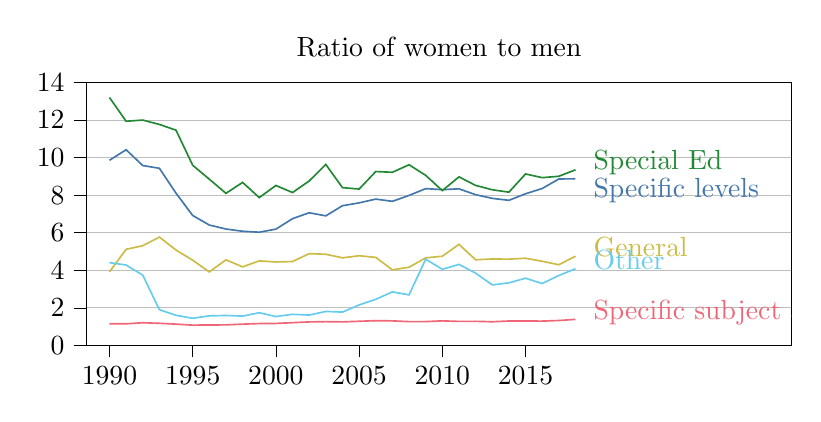
\begin{tikzpicture}

\definecolor{color0}{rgb}{0.266666666666667,0.466666666666667,0.666666666666667}
\definecolor{color1}{rgb}{0.933333333333333,0.4,0.466666666666667}
\definecolor{color2}{rgb}{0.133333333333333,0.533333333333333,0.2}
\definecolor{color3}{rgb}{0.8,0.733333333333333,0.266666666666667}
\definecolor{color4}{rgb}{0.4,0.8,0.933333333333333}

\begin{axis}[
height=140pt,
tick align=outside,
tick pos=left,
title={Ratio of women to men},
width=300pt,
x grid style={white!69.0196078431373!black},
xmin=1988.6, xmax=2031,
xtick style={color=black},
xtick={1990,1995,2000,2005,2010,2015},
xticklabels={\(\displaystyle 1990\),\(\displaystyle 1995\),\(\displaystyle 2000\),\(\displaystyle 2005\),\(\displaystyle 2010\),\(\displaystyle 2015\)},
ymajorgrids,
ymin=0, ymax=14,
ytick style={color=black},
ytick={0,2,4,6,8,10,12,14},
yticklabels={\(\displaystyle 0\),\(\displaystyle 2\),\(\displaystyle 4\),\(\displaystyle 6\),\(\displaystyle 8\),\(\displaystyle 10\),\(\displaystyle 12\),\(\displaystyle 14\)}
]
\addplot [semithick, color0]
table {%
1990 9.85678482055664
1991 10.4184417724609
1992 9.57731819152832
1993 9.43160533905029
1994 8.10525512695312
1995 6.9180326461792
1996 6.40954542160034
1997 6.19707584381104
1998 6.07839679718018
1999 6.02802467346191
2000 6.19081592559814
2001 6.74944686889648
2002 7.06294870376587
2003 6.89906072616577
2004 7.43850517272949
2005 7.58988857269287
2006 7.79117202758789
2007 7.67146778106689
2008 7.98672437667847
2009 8.34756278991699
2010 8.29460144042969
2011 8.33722496032715
2012 8.02534294128418
2013 7.83027839660645
2014 7.72595024108887
2015 8.07444095611572
2016 8.35525131225586
2017 8.86260604858398
2018 8.87155628204346
};
\addplot [semithick, color1]
table {%
1990 1.15532171726227
1991 1.15024888515472
1992 1.20649778842926
1993 1.1759877204895
1994 1.1329128742218
1995 1.07971060276031
1997 1.09327447414398
1998 1.13211607933044
1999 1.16261231899261
2000 1.17057001590729
2002 1.25058615207672
2003 1.2647932767868
2004 1.2525497674942
2006 1.31692135334015
2007 1.3057245016098
2008 1.26573371887207
2009 1.26778817176819
2010 1.30617690086365
2011 1.27807295322418
2012 1.28198528289795
2013 1.25922918319702
2014 1.29929637908936
2016 1.29459202289581
2017 1.32512831687927
2018 1.38676393032074
};
\addplot [semithick, color2]
table {%
1990 13.2028684616089
1991 11.9372758865356
1992 11.9983997344971
1993 11.7669067382812
1994 11.4590606689453
1995 9.59314727783203
1996 8.85048580169678
1997 8.09811019897461
1998 8.68064785003662
1999 7.87073612213135
2000 8.5166015625
2001 8.13870620727539
2002 8.75614738464355
2003 9.63495826721191
2004 8.40132331848145
2005 8.32505416870117
2006 9.25802612304688
2007 9.21923923492432
2008 9.6187572479248
2009 9.05656147003174
2010 8.24395179748535
2011 8.97454929351807
2012 8.51985263824463
2013 8.28767108917236
2014 8.15909099578857
2015 9.13000965118408
2016 8.93281364440918
2017 9.00601196289062
2018 9.35100746154785
};
\addplot [semithick, color3]
table {%
1990 3.91208791732788
1991 5.11620807647705
1992 5.30857133865356
1993 5.76821184158325
1994 5.07865190505981
1995 4.53516817092896
1996 3.91124248504639
1997 4.55709362030029
1998 4.18258428573608
1999 4.50142431259155
2000 4.44356966018677
2001 4.46636772155762
2002 4.8848614692688
2003 4.85388994216919
2004 4.66360282897949
2005 4.77389287948608
2006 4.68814945220947
2007 4.02201843261719
2008 4.16236162185669
2009 4.6621880531311
2010 4.74836587905884
2011 5.38130855560303
2012 4.5588698387146
2013 4.60235643386841
2014 4.59259271621704
2015 4.64153289794922
2016 4.47950839996338
2017 4.29462099075317
2018 4.74932241439819
};
\addplot [semithick, color4]
table {%
1990 4.40740728378296
1991 4.28019332885742
1992 3.74193549156189
1993 1.90348529815674
1994 1.60401463508606
1995 1.44357371330261
1996 1.57372260093689
1997 1.59370529651642
1998 1.55980062484741
1999 1.74101793766022
2000 1.53652060031891
2001 1.65552699565887
2002 1.61428570747375
2003 1.80882358551025
2004 1.77362632751465
2005 2.15558052062988
2006 2.45138049125671
2007 2.84980750083923
2008 2.69146013259888
2009 4.59161138534546
2010 4.0516529083252
2011 4.31400012969971
2012 3.84789633750916
2013 3.22127652168274
2014 3.33093523979187
2015 3.57739949226379
2016 3.29508185386658
2017 3.72172617912292
2018 4.08270692825317
};
\draw (axis cs:2018.5,7.87155599603568) node[
  anchor=base west,
  text=color0,
  rotate=0.0
]{Specific levels};
\draw (axis cs:2018.5,1.38676388109927) node[
  anchor=base west,
  text=color1,
  rotate=0.0
]{Specific subject area};
\draw (axis cs:2018.5,9.35100742311771) node[
  anchor=base west,
  text=color2,
  rotate=0.0
]{Special Ed};
\draw (axis cs:2018.5,4.74932249322493) node[
  anchor=base west,
  text=color3,
  rotate=0.0
]{General};
\draw (axis cs:2018.5,4.03270676691729) node[
  anchor=base west,
  text=color4,
  rotate=0.0
]{Other};
\end{axis}

\end{tikzpicture}

\vspace{0.1cm}
\begin{tikzpicture}
% This file was created by tikzplotlib v0.9.2.
\definecolor{color0}{rgb}{0.266666666666667,0.466666666666667,0.666666666666667}
\definecolor{color1}{rgb}{0.933333333333333,0.4,0.466666666666667}
\definecolor{color2}{rgb}{0.133333333333333,0.533333333333333,0.2}
\definecolor{color3}{rgb}{0.8,0.733333333333333,0.266666666666667}
\definecolor{color4}{rgb}{0.4,0.8,0.933333333333333}

\begin{groupplot}[group style={group size=2 by 1, group name=my plots, horizontal sep=0.8cm}]
\nextgroupplot[
height=90pt, width=160pt,
legend style={at={(2.02, 0.5)},anchor=west,},
reverse legend,
tick align=outside,
tick pos=left,
x grid style={white!69.0196078431373!black},
xlabel={Women},
xmin=1988.6, xmax=2019.4,
xtick style={color=black},
xtick={1990,2000,2010},
xticklabels={\(\displaystyle 1990\),\(\displaystyle 2000\),\(\displaystyle 2010\)},
ymajorgrids,
ymin=0, ymax=95.61825,
ytick style={color=black}
]
\path [draw=color0, fill=color0]
(axis cs:1990,55.129)
--(axis cs:1990,0)
--(axis cs:1991,0)
--(axis cs:1992,0)
--(axis cs:1993,0)
--(axis cs:1994,0)
--(axis cs:1995,0)
--(axis cs:1996,0)
--(axis cs:1997,0)
--(axis cs:1998,0)
--(axis cs:1999,0)
--(axis cs:2000,0)
--(axis cs:2001,0)
--(axis cs:2002,0)
--(axis cs:2003,0)
--(axis cs:2004,0)
--(axis cs:2005,0)
--(axis cs:2006,0)
--(axis cs:2007,0)
--(axis cs:2008,0)
--(axis cs:2009,0)
--(axis cs:2010,0)
--(axis cs:2011,0)
--(axis cs:2012,0)
--(axis cs:2013,0)
--(axis cs:2014,0)
--(axis cs:2015,0)
--(axis cs:2016,0)
--(axis cs:2017,0)
--(axis cs:2018,0)
--(axis cs:2018,44.757)
--(axis cs:2018,44.757)
--(axis cs:2017,46.121)
--(axis cs:2016,46.38)
--(axis cs:2015,48.051)
--(axis cs:2014,52.042)
--(axis cs:2013,55.963)
--(axis cs:2012,57.317)
--(axis cs:2011,57.135)
--(axis cs:2010,55.466)
--(axis cs:2009,56.513)
--(axis cs:2008,57.153)
--(axis cs:2007,58.587)
--(axis cs:2006,60.366)
--(axis cs:2005,59.148)
--(axis cs:2004,58.727)
--(axis cs:2003,52.15)
--(axis cs:2002,56.101)
--(axis cs:2001,54.927)
--(axis cs:2000,53.792)
--(axis cs:1999,52.914)
--(axis cs:1998,51.405)
--(axis cs:1997,51.287)
--(axis cs:1996,51.302)
--(axis cs:1995,52.75)
--(axis cs:1994,55.367)
--(axis cs:1993,56.401)
--(axis cs:1992,57.847)
--(axis cs:1991,59.656)
--(axis cs:1990,55.129)
--cycle;

\path [draw=color1, fill=color1]
(axis cs:1990,74.342)
--(axis cs:1990,55.129)
--(axis cs:1991,59.656)
--(axis cs:1992,57.847)
--(axis cs:1993,56.401)
--(axis cs:1994,55.367)
--(axis cs:1995,52.75)
--(axis cs:1996,51.302)
--(axis cs:1997,51.287)
--(axis cs:1998,51.405)
--(axis cs:1999,52.914)
--(axis cs:2000,53.792)
--(axis cs:2001,54.927)
--(axis cs:2002,56.101)
--(axis cs:2003,52.15)
--(axis cs:2004,58.727)
--(axis cs:2005,59.148)
--(axis cs:2006,60.366)
--(axis cs:2007,58.587)
--(axis cs:2008,57.153)
--(axis cs:2009,56.513)
--(axis cs:2010,55.466)
--(axis cs:2011,57.135)
--(axis cs:2012,57.317)
--(axis cs:2013,55.963)
--(axis cs:2014,52.042)
--(axis cs:2015,48.051)
--(axis cs:2016,46.38)
--(axis cs:2017,46.121)
--(axis cs:2018,44.757)
--(axis cs:2018,57.12)
--(axis cs:2018,57.12)
--(axis cs:2017,58.772)
--(axis cs:2016,60.025)
--(axis cs:2015,62.74)
--(axis cs:2014,67.922)
--(axis cs:2013,73.018)
--(axis cs:2012,74.752)
--(axis cs:2011,74.697)
--(axis cs:2010,73.102)
--(axis cs:2009,74.224)
--(axis cs:2008,74.972)
--(axis cs:2007,77.268)
--(axis cs:2006,78.982)
--(axis cs:2005,77.085)
--(axis cs:2004,76.289)
--(axis cs:2003,69.613)
--(axis cs:2002,74.771)
--(axis cs:2001,73.56)
--(axis cs:2000,72.335)
--(axis cs:1999,71.41)
--(axis cs:1998,69.82)
--(axis cs:1997,69.103)
--(axis cs:1996,69.404)
--(axis cs:1995,70.657)
--(axis cs:1994,74.051)
--(axis cs:1993,75.599)
--(axis cs:1992,77.046)
--(axis cs:1991,79.063)
--(axis cs:1990,74.342)
--cycle;

\path [draw=color2, fill=color2]
(axis cs:1990,80.785)
--(axis cs:1990,74.342)
--(axis cs:1991,79.063)
--(axis cs:1992,77.046)
--(axis cs:1993,75.599)
--(axis cs:1994,74.051)
--(axis cs:1995,70.657)
--(axis cs:1996,69.404)
--(axis cs:1997,69.103)
--(axis cs:1998,69.82)
--(axis cs:1999,71.41)
--(axis cs:2000,72.335)
--(axis cs:2001,73.56)
--(axis cs:2002,74.771)
--(axis cs:2003,69.613)
--(axis cs:2004,76.289)
--(axis cs:2005,77.085)
--(axis cs:2006,78.982)
--(axis cs:2007,77.268)
--(axis cs:2008,74.972)
--(axis cs:2009,74.224)
--(axis cs:2010,73.102)
--(axis cs:2011,74.697)
--(axis cs:2012,74.752)
--(axis cs:2013,73.018)
--(axis cs:2014,67.922)
--(axis cs:2015,62.74)
--(axis cs:2016,60.025)
--(axis cs:2017,58.772)
--(axis cs:2018,57.12)
--(axis cs:2018,65.938)
--(axis cs:2018,65.938)
--(axis cs:2017,67.76)
--(axis cs:2016,69.199)
--(axis cs:2015,72.08)
--(axis cs:2014,77.615)
--(axis cs:2013,82.698)
--(axis cs:2012,83.979)
--(axis cs:2011,83.16)
--(axis cs:2010,81.28)
--(axis cs:2009,82.23)
--(axis cs:2008,82.869)
--(axis cs:2007,85.51)
--(axis cs:2006,86.768)
--(axis cs:2005,84.794)
--(axis cs:2004,83.909)
--(axis cs:2003,77.716)
--(axis cs:2002,83.317)
--(axis cs:2001,82.244)
--(axis cs:2000,81.056)
--(axis cs:1999,80.178)
--(axis cs:1998,78.926)
--(axis cs:1997,78.1)
--(axis cs:1996,78.52)
--(axis cs:1995,79.617)
--(axis cs:1994,82.588)
--(axis cs:1993,83.777)
--(axis cs:1992,84.545)
--(axis cs:1991,85.724)
--(axis cs:1990,80.785)
--cycle;

\path [draw=color3, fill=color3]
(axis cs:1990,82.565)
--(axis cs:1990,80.785)
--(axis cs:1991,85.724)
--(axis cs:1992,84.545)
--(axis cs:1993,83.777)
--(axis cs:1994,82.588)
--(axis cs:1995,79.617)
--(axis cs:1996,78.52)
--(axis cs:1997,78.1)
--(axis cs:1998,78.926)
--(axis cs:1999,80.178)
--(axis cs:2000,81.056)
--(axis cs:2001,82.244)
--(axis cs:2002,83.317)
--(axis cs:2003,77.716)
--(axis cs:2004,83.909)
--(axis cs:2005,84.794)
--(axis cs:2006,86.768)
--(axis cs:2007,85.51)
--(axis cs:2008,82.869)
--(axis cs:2009,82.23)
--(axis cs:2010,81.28)
--(axis cs:2011,83.16)
--(axis cs:2012,83.979)
--(axis cs:2013,82.698)
--(axis cs:2014,77.615)
--(axis cs:2015,72.08)
--(axis cs:2016,69.199)
--(axis cs:2017,67.76)
--(axis cs:2018,65.938)
--(axis cs:2018,69.443)
--(axis cs:2018,69.443)
--(axis cs:2017,71.273)
--(axis cs:2016,72.478)
--(axis cs:2015,75.835)
--(axis cs:2014,81.087)
--(axis cs:2013,85.823)
--(axis cs:2012,86.883)
--(axis cs:2011,86.039)
--(axis cs:2010,84.186)
--(axis cs:2009,84.659)
--(axis cs:2008,85.125)
--(axis cs:2007,87.702)
--(axis cs:2006,89.023)
--(axis cs:2005,86.842)
--(axis cs:2004,86.446)
--(axis cs:2003,80.274)
--(axis cs:2002,85.608)
--(axis cs:2001,84.236)
--(axis cs:2000,82.749)
--(axis cs:1999,81.758)
--(axis cs:1998,80.415)
--(axis cs:1997,79.417)
--(axis cs:1996,79.842)
--(axis cs:1995,81.1)
--(axis cs:1994,83.944)
--(axis cs:1993,85.519)
--(axis cs:1992,86.403)
--(axis cs:1991,87.397)
--(axis cs:1990,82.565)
--cycle;

\path [draw=color4, fill=color4]
(axis cs:1990,83.993)
--(axis cs:1990,82.565)
--(axis cs:1991,87.397)
--(axis cs:1992,86.403)
--(axis cs:1993,85.519)
--(axis cs:1994,83.944)
--(axis cs:1995,81.1)
--(axis cs:1996,79.842)
--(axis cs:1997,79.417)
--(axis cs:1998,80.415)
--(axis cs:1999,81.758)
--(axis cs:2000,82.749)
--(axis cs:2001,84.236)
--(axis cs:2002,85.608)
--(axis cs:2003,80.274)
--(axis cs:2004,86.446)
--(axis cs:2005,86.842)
--(axis cs:2006,89.023)
--(axis cs:2007,87.702)
--(axis cs:2008,85.125)
--(axis cs:2009,84.659)
--(axis cs:2010,84.186)
--(axis cs:2011,86.039)
--(axis cs:2012,86.883)
--(axis cs:2013,85.823)
--(axis cs:2014,81.087)
--(axis cs:2015,75.835)
--(axis cs:2016,72.478)
--(axis cs:2017,71.273)
--(axis cs:2018,69.443)
--(axis cs:2018,72.158)
--(axis cs:2018,72.158)
--(axis cs:2017,73.774)
--(axis cs:2016,74.89)
--(axis cs:2015,78.146)
--(axis cs:2014,83.402)
--(axis cs:2013,88.094)
--(axis cs:2012,89.261)
--(axis cs:2011,88.196)
--(axis cs:2010,86.147)
--(axis cs:2009,86.739)
--(axis cs:2008,87.079)
--(axis cs:2007,89.922)
--(axis cs:2006,91.065)
--(axis cs:2005,88.754)
--(axis cs:2004,88.06)
--(axis cs:2003,81.75)
--(axis cs:2002,87.077)
--(axis cs:2001,85.524)
--(axis cs:2000,83.906)
--(axis cs:1999,82.921)
--(axis cs:1998,81.354)
--(axis cs:1997,80.531)
--(axis cs:1996,80.92)
--(axis cs:1995,82.021)
--(axis cs:1994,84.823)
--(axis cs:1993,86.229)
--(axis cs:1992,87.215)
--(axis cs:1991,89.169)
--(axis cs:1990,83.993)
--cycle;

\addplot [semithick, color0]
table {%
1990 55.1290016174316
1991 59.6559982299805
1992 57.8470001220703
1993 56.4010009765625
1994 55.367000579834
1995 52.75
1996 51.3019981384277
1997 51.2869987487793
1998 51.4049987792969
1999 52.9140014648438
2000 53.7919998168945
2001 54.9269981384277
2002 56.101001739502
2003 52.1500015258789
2004 58.7270011901855
2005 59.1479988098145
2006 60.3660011291504
2007 58.5870018005371
2008 57.1529998779297
2009 56.5130004882812
2010 55.4659996032715
2011 57.1349983215332
2012 57.3170013427734
2013 55.9630012512207
2014 52.0419998168945
2015 48.0509986877441
2016 46.3800010681152
2017 46.1209983825684
2018 44.7569999694824
};
\addplot [semithick, color1]
table {%
1990 74.3420028686523
1991 79.0630035400391
1992 77.0459976196289
1993 75.5989990234375
1994 74.0510025024414
1995 70.6569976806641
1996 69.4039993286133
1997 69.1029968261719
1998 69.8199996948242
1999 71.4100036621094
2000 72.3349990844727
2001 73.5599975585938
2002 74.7710037231445
2003 69.6129989624023
2004 76.2890014648438
2005 77.0849990844727
2006 78.9820022583008
2007 77.2679977416992
2008 74.9720001220703
2009 74.2239990234375
2010 73.1019973754883
2011 74.6969985961914
2012 74.7519989013672
2013 73.0179977416992
2014 67.9219970703125
2015 62.7400016784668
2016 60.0250015258789
2017 58.7719993591309
2018 57.1199989318848
};
\addplot [semithick, color2]
table {%
1990 80.7850036621094
1991 85.7239990234375
1992 84.5449981689453
1993 83.7770004272461
1994 82.5879974365234
1995 79.6169967651367
1996 78.5199966430664
1997 78.0999984741211
1998 78.9260025024414
1999 80.1780014038086
2000 81.0559997558594
2001 82.2440032958984
2002 83.3170013427734
2003 77.7160034179688
2004 83.9089965820312
2005 84.7939987182617
2006 86.7679977416992
2007 85.5100021362305
2008 82.8690032958984
2009 82.2300033569336
2010 81.2799987792969
2011 83.1600036621094
2012 83.9789962768555
2013 82.697998046875
2014 77.6149978637695
2015 72.0800018310547
2016 69.1989974975586
2017 67.7600021362305
2018 65.9380035400391
};
\addplot [semithick, color3]
table {%
1990 82.5650024414062
1991 87.3970031738281
1992 86.4029998779297
1993 85.5189971923828
1994 83.9440002441406
1995 81.0999984741211
1996 79.8420028686523
1997 79.4169998168945
1998 80.4150009155273
1999 81.7580032348633
2000 82.7490005493164
2001 84.2360000610352
2002 85.6080017089844
2003 80.2740020751953
2004 86.4459991455078
2005 86.8420028686523
2006 89.0230026245117
2007 87.7020034790039
2008 85.125
2010 84.1859970092773
2011 86.0390014648438
2012 86.8830032348633
2013 85.822998046875
2014 81.0869979858398
2015 75.8349990844727
2016 72.4779968261719
2017 71.2730026245117
2018 69.443000793457
};
\addplot [semithick, color4]
table {%
1990 83.9929962158203
1991 89.1689987182617
1992 87.2149963378906
1993 86.2289962768555
1994 84.822998046875
1995 82.0210037231445
1996 80.9199981689453
1997 80.5309982299805
1998 81.3539962768555
1999 82.9209976196289
2000 83.9059982299805
2001 85.5240020751953
2002 87.0770034790039
2003 81.75
2004 88.0599975585938
2005 88.7539978027344
2006 91.0650024414062
2007 89.9219970703125
2008 87.0790023803711
2009 86.7389984130859
2010 86.1470031738281
2011 88.1959991455078
2012 89.2610015869141
2013 88.0940017700195
2014 83.4020004272461
2015 78.1460037231445
2016 74.8899993896484
2017 73.7740020751953
2018 72.1579971313477
};

\nextgroupplot[
height=90pt, width=160pt,
legend style={at={(2.02, 0.5)},anchor=west,},
reverse legend,
tick align=outside,
tick pos=left,
x grid style={white!69.0196078431373!black},
xlabel={Men},
xmin=1988.6, xmax=2019.4,
xtick style={color=black},
xtick={1990,2000,2010},
xticklabels={\(\displaystyle 1990\),\(\displaystyle 2000\),\(\displaystyle 2010\)},
ymajorgrids,
ymin=0, ymax=28.161,
ytick style={color=black}
]
\path [draw=color0, fill=color0]
(axis cs:1990,5.593)
--(axis cs:1990,0)
--(axis cs:1991,0)
--(axis cs:1992,0)
--(axis cs:1993,0)
--(axis cs:1994,0)
--(axis cs:1995,0)
--(axis cs:1996,0)
--(axis cs:1997,0)
--(axis cs:1998,0)
--(axis cs:1999,0)
--(axis cs:2000,0)
--(axis cs:2001,0)
--(axis cs:2002,0)
--(axis cs:2003,0)
--(axis cs:2004,0)
--(axis cs:2005,0)
--(axis cs:2006,0)
--(axis cs:2007,0)
--(axis cs:2008,0)
--(axis cs:2009,0)
--(axis cs:2010,0)
--(axis cs:2011,0)
--(axis cs:2012,0)
--(axis cs:2013,0)
--(axis cs:2014,0)
--(axis cs:2015,0)
--(axis cs:2016,0)
--(axis cs:2017,0)
--(axis cs:2018,0)
--(axis cs:2018,5.045)
--(axis cs:2018,5.045)
--(axis cs:2017,5.204)
--(axis cs:2016,5.551)
--(axis cs:2015,5.951)
--(axis cs:2014,6.736)
--(axis cs:2013,7.147)
--(axis cs:2012,7.142)
--(axis cs:2011,6.853)
--(axis cs:2010,6.687)
--(axis cs:2009,6.77)
--(axis cs:2008,7.156)
--(axis cs:2007,7.637)
--(axis cs:2006,7.748)
--(axis cs:2005,7.793)
--(axis cs:2004,7.895)
--(axis cs:2003,7.559)
--(axis cs:2002,7.943)
--(axis cs:2001,8.138)
--(axis cs:2000,8.689)
--(axis cs:1999,8.778)
--(axis cs:1998,8.457)
--(axis cs:1997,8.276)
--(axis cs:1996,8.004)
--(axis cs:1995,7.625)
--(axis cs:1994,6.831)
--(axis cs:1993,5.98)
--(axis cs:1992,6.04)
--(axis cs:1991,5.726)
--(axis cs:1990,5.593)
--cycle;

\path [draw=color1, fill=color1]
(axis cs:1990,22.223)
--(axis cs:1990,5.593)
--(axis cs:1991,5.726)
--(axis cs:1992,6.04)
--(axis cs:1993,5.98)
--(axis cs:1994,6.831)
--(axis cs:1995,7.625)
--(axis cs:1996,8.004)
--(axis cs:1997,8.276)
--(axis cs:1998,8.457)
--(axis cs:1999,8.778)
--(axis cs:2000,8.689)
--(axis cs:2001,8.138)
--(axis cs:2002,7.943)
--(axis cs:2003,7.559)
--(axis cs:2004,7.895)
--(axis cs:2005,7.793)
--(axis cs:2006,7.748)
--(axis cs:2007,7.637)
--(axis cs:2008,7.156)
--(axis cs:2009,6.77)
--(axis cs:2010,6.687)
--(axis cs:2011,6.853)
--(axis cs:2012,7.142)
--(axis cs:2013,7.147)
--(axis cs:2014,6.736)
--(axis cs:2015,5.951)
--(axis cs:2016,5.551)
--(axis cs:2017,5.204)
--(axis cs:2018,5.045)
--(axis cs:2018,13.96)
--(axis cs:2018,13.96)
--(axis cs:2017,14.751)
--(axis cs:2016,16.091)
--(axis cs:2015,17.272)
--(axis cs:2014,18.958)
--(axis cs:2013,20.691)
--(axis cs:2012,20.742)
--(axis cs:2011,20.594)
--(axis cs:2010,20.189)
--(axis cs:2009,20.74)
--(axis cs:2008,21.234)
--(axis cs:2007,21.944)
--(axis cs:2006,21.884)
--(axis cs:2005,21.766)
--(axis cs:2004,21.916)
--(axis cs:2003,21.366)
--(axis cs:2002,22.872)
--(axis cs:2001,23.53)
--(axis cs:2000,24.53)
--(axis cs:1999,24.687)
--(axis cs:1998,24.723)
--(axis cs:1997,24.572)
--(axis cs:1996,24.651)
--(axis cs:1995,24.21)
--(axis cs:1994,23.323)
--(axis cs:1993,22.305)
--(axis cs:1992,21.953)
--(axis cs:1991,22.598)
--(axis cs:1990,22.223)
--cycle;

\path [draw=color2, fill=color2]
(axis cs:1990,22.711)
--(axis cs:1990,22.223)
--(axis cs:1991,22.598)
--(axis cs:1992,21.953)
--(axis cs:1993,22.305)
--(axis cs:1994,23.323)
--(axis cs:1995,24.21)
--(axis cs:1996,24.651)
--(axis cs:1997,24.572)
--(axis cs:1998,24.723)
--(axis cs:1999,24.687)
--(axis cs:2000,24.53)
--(axis cs:2001,23.53)
--(axis cs:2002,22.872)
--(axis cs:2003,21.366)
--(axis cs:2004,21.916)
--(axis cs:2005,21.766)
--(axis cs:2006,21.884)
--(axis cs:2007,21.944)
--(axis cs:2008,21.234)
--(axis cs:2009,20.74)
--(axis cs:2010,20.189)
--(axis cs:2011,20.594)
--(axis cs:2012,20.742)
--(axis cs:2013,20.691)
--(axis cs:2014,18.958)
--(axis cs:2015,17.272)
--(axis cs:2016,16.091)
--(axis cs:2017,14.751)
--(axis cs:2018,13.96)
--(axis cs:2018,14.903)
--(axis cs:2018,14.903)
--(axis cs:2017,15.749)
--(axis cs:2016,17.118)
--(axis cs:2015,18.295)
--(axis cs:2014,20.146)
--(axis cs:2013,21.859)
--(axis cs:2012,21.825)
--(axis cs:2011,21.537)
--(axis cs:2010,21.181)
--(axis cs:2009,21.624)
--(axis cs:2008,22.055)
--(axis cs:2007,22.838)
--(axis cs:2006,22.725)
--(axis cs:2005,22.692)
--(axis cs:2004,22.823)
--(axis cs:2003,22.207)
--(axis cs:2002,23.848)
--(axis cs:2001,24.597)
--(axis cs:2000,25.554)
--(axis cs:1999,25.801)
--(axis cs:1998,25.772)
--(axis cs:1997,25.683)
--(axis cs:1996,25.681)
--(axis cs:1995,25.144)
--(axis cs:1994,24.068)
--(axis cs:1993,23)
--(axis cs:1992,22.578)
--(axis cs:1991,23.156)
--(axis cs:1990,22.711)
--cycle;

\path [draw=color3, fill=color3]
(axis cs:1990,23.166)
--(axis cs:1990,22.711)
--(axis cs:1991,23.156)
--(axis cs:1992,22.578)
--(axis cs:1993,23)
--(axis cs:1994,24.068)
--(axis cs:1995,25.144)
--(axis cs:1996,25.681)
--(axis cs:1997,25.683)
--(axis cs:1998,25.772)
--(axis cs:1999,25.801)
--(axis cs:2000,25.554)
--(axis cs:2001,24.597)
--(axis cs:2002,23.848)
--(axis cs:2003,22.207)
--(axis cs:2004,22.823)
--(axis cs:2005,22.692)
--(axis cs:2006,22.725)
--(axis cs:2007,22.838)
--(axis cs:2008,22.055)
--(axis cs:2009,21.624)
--(axis cs:2010,21.181)
--(axis cs:2011,21.537)
--(axis cs:2012,21.825)
--(axis cs:2013,21.859)
--(axis cs:2014,20.146)
--(axis cs:2015,18.295)
--(axis cs:2016,17.118)
--(axis cs:2017,15.749)
--(axis cs:2018,14.903)
--(axis cs:2018,15.641)
--(axis cs:2018,15.641)
--(axis cs:2017,16.567)
--(axis cs:2016,17.85)
--(axis cs:2015,19.104)
--(axis cs:2014,20.902)
--(axis cs:2013,22.538)
--(axis cs:2012,22.462)
--(axis cs:2011,22.072)
--(axis cs:2010,21.793)
--(axis cs:2009,22.145)
--(axis cs:2008,22.597)
--(axis cs:2007,23.383)
--(axis cs:2006,23.206)
--(axis cs:2005,23.121)
--(axis cs:2004,23.367)
--(axis cs:2003,22.734)
--(axis cs:2002,24.317)
--(axis cs:2001,25.043)
--(axis cs:2000,25.935)
--(axis cs:1999,26.152)
--(axis cs:1998,26.128)
--(axis cs:1997,25.972)
--(axis cs:1996,26.019)
--(axis cs:1995,25.471)
--(axis cs:1994,24.335)
--(axis cs:1993,23.302)
--(axis cs:1992,22.928)
--(axis cs:1991,23.483)
--(axis cs:1990,23.166)
--cycle;

\path [draw=color4, fill=color4]
(axis cs:1990,23.49)
--(axis cs:1990,23.166)
--(axis cs:1991,23.483)
--(axis cs:1992,22.928)
--(axis cs:1993,23.302)
--(axis cs:1994,24.335)
--(axis cs:1995,25.471)
--(axis cs:1996,26.019)
--(axis cs:1997,25.972)
--(axis cs:1998,26.128)
--(axis cs:1999,26.152)
--(axis cs:2000,25.935)
--(axis cs:2001,25.043)
--(axis cs:2002,24.317)
--(axis cs:2003,22.734)
--(axis cs:2004,23.367)
--(axis cs:2005,23.121)
--(axis cs:2006,23.206)
--(axis cs:2007,23.383)
--(axis cs:2008,22.597)
--(axis cs:2009,22.145)
--(axis cs:2010,21.793)
--(axis cs:2011,22.072)
--(axis cs:2012,22.462)
--(axis cs:2013,22.538)
--(axis cs:2014,20.902)
--(axis cs:2015,19.104)
--(axis cs:2016,17.85)
--(axis cs:2017,16.567)
--(axis cs:2018,15.641)
--(axis cs:2018,16.306)
--(axis cs:2018,16.306)
--(axis cs:2017,17.239)
--(axis cs:2016,18.582)
--(axis cs:2015,19.75)
--(axis cs:2014,21.597)
--(axis cs:2013,23.243)
--(axis cs:2012,23.08)
--(axis cs:2011,22.572)
--(axis cs:2010,22.277)
--(axis cs:2009,22.598)
--(axis cs:2008,23.323)
--(axis cs:2007,24.162)
--(axis cs:2006,24.039)
--(axis cs:2005,24.008)
--(axis cs:2004,24.277)
--(axis cs:2003,23.55)
--(axis cs:2002,25.227)
--(axis cs:2001,25.821)
--(axis cs:2000,26.688)
--(axis cs:1999,26.82)
--(axis cs:1998,26.73)
--(axis cs:1997,26.671)
--(axis cs:1996,26.704)
--(axis cs:1995,26.109)
--(axis cs:1994,24.883)
--(axis cs:1993,23.675)
--(axis cs:1992,23.145)
--(axis cs:1991,23.897)
--(axis cs:1990,23.49)
--cycle;

\addplot [semithick, color0]
table {%
1990 5.59299993515015
1991 5.72599983215332
1992 6.03999996185303
1993 5.98000001907349
1994 6.83099985122681
1995 7.625
1996 8.00399971008301
1997 8.27600002288818
1998 8.45699977874756
1999 8.77799987792969
2000 8.68900012969971
2001 8.13799953460693
2002 7.94299983978271
2003 7.55900001525879
2004 7.89499998092651
2005 7.79300022125244
2006 7.7480001449585
2007 7.63700008392334
2008 7.1560001373291
2009 6.76999998092651
2010 6.68699979782104
2011 6.85300016403198
2012 7.14200019836426
2013 7.14699983596802
2014 6.73600006103516
2015 5.95100021362305
2016 5.55100011825562
2017 5.2039999961853
2018 5.04500007629395
};
\addplot [semithick, color1]
table {%
1990 22.2229995727539
1991 22.5979995727539
1992 21.9529991149902
1993 22.3050003051758
1994 23.3229999542236
1995 24.2099990844727
1996 24.6509990692139
1997 24.57200050354
1998 24.7229995727539
1999 24.6870002746582
2000 24.5300006866455
2001 23.5300006866455
2002 22.8719997406006
2003 21.3659992218018
2004 21.9160003662109
2005 21.7660007476807
2006 21.8840007781982
2007 21.9440002441406
2008 21.2339992523193
2009 20.7399997711182
2010 20.1889991760254
2011 20.5939998626709
2012 20.742000579834
2013 20.6909999847412
2014 18.9580001831055
2015 17.2719993591309
2016 16.0909996032715
2017 14.7510004043579
2018 13.960000038147
};
\addplot [semithick, color2]
table {%
1990 22.7110004425049
1991 23.1560001373291
1992 22.5779991149902
1993 23
1995 25.1439990997314
1996 25.6809997558594
1997 25.6830005645752
1998 25.7719993591309
1999 25.8010005950928
2000 25.5540008544922
2001 24.5970001220703
2002 23.8479995727539
2003 22.2070007324219
2004 22.8229999542236
2005 22.6919994354248
2006 22.7250003814697
2007 22.8379993438721
2008 22.0550003051758
2009 21.6240005493164
2010 21.1809997558594
2011 21.5370006561279
2012 21.8250007629395
2013 21.8589992523193
2014 20.1459999084473
2015 18.2950000762939
2016 17.1180000305176
2017 15.7489995956421
2018 14.9029998779297
};
\addplot [semithick, color3]
table {%
1990 23.1660003662109
1991 23.4829998016357
1992 22.92799949646
1993 23.3020000457764
1994 24.3349990844727
1995 25.4710006713867
1996 26.0189990997314
1997 25.9720001220703
1998 26.1280002593994
1999 26.1520004272461
2000 25.9349994659424
2001 25.0429992675781
2002 24.3169994354248
2003 22.7339992523193
2004 23.367000579834
2005 23.121000289917
2006 23.2059993743896
2007 23.382999420166
2008 22.5970001220703
2009 22.1450004577637
2010 21.7929992675781
2011 22.07200050354
2012 22.4619998931885
2013 22.5380001068115
2014 20.9020004272461
2015 19.1040000915527
2016 17.8500003814697
2017 16.5669994354248
2018 15.6409997940063
};
\addplot [semithick, color4]
table {%
1990 23.4899997711182
1991 23.8969993591309
1992 23.1450004577637
1993 23.6749992370605
1994 24.882999420166
1995 26.1089992523193
1996 26.7040004730225
1997 26.6709995269775
1998 26.7299995422363
1999 26.8199996948242
2000 26.6879997253418
2001 25.8209991455078
2002 25.2269992828369
2003 23.5499992370605
2004 24.2770004272461
2005 24.007999420166
2006 24.0389995574951
2007 24.1620006561279
2008 23.3229999542236
2009 22.5979995727539
2010 22.2770004272461
2011 22.57200050354
2012 23.0799999237061
2013 23.2430000305176
2014 21.5970001220703
2015 19.75
2016 18.5820007324219
2017 17.2390003204346
2018 16.3059997558594
};
\end{groupplot}




\end{tikzpicture}
\caption{Number Bachelor's degrees awarded (thousands). Source: IPEDS.}

\end{figure}
\hyperlink{intro_social_science_ratio}{\beamerbutton{Return: Social science ratio}}
}
\end{frame}

%%%%%%%%%%%%%%%%%%%%%%%%%%%%%%%%%%%%%%%%%%%%%%%%%%%%%%%%%%%%%%%%%%%%%%%%%%%%%%%%
\begin{frame}{Biological and Physical Sciences and Mathematics}\label{app_science_math}
\Wider[4em]{

\begin{figure}
\setlength{\abovecaptionskip}{2pt}
\setlength{\belowcaptionskip}{-2pt}
% This file was created by tikzplotlib v0.9.2.
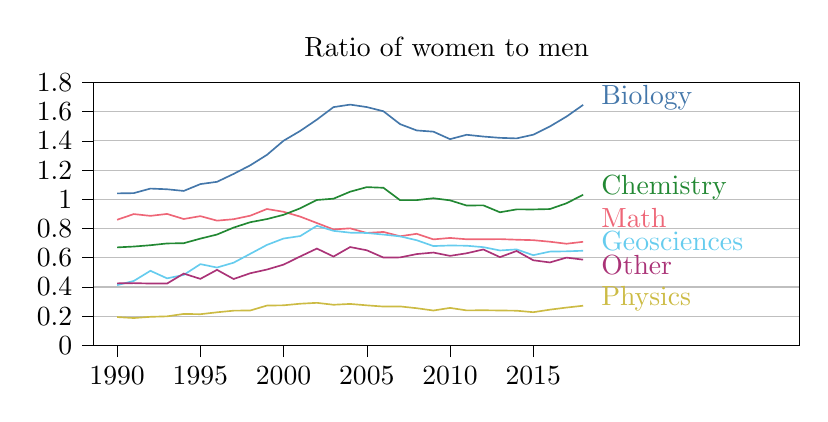
\begin{tikzpicture}

\definecolor{color0}{rgb}{0.266666666666667,0.466666666666667,0.666666666666667}
\definecolor{color1}{rgb}{0.933333333333333,0.4,0.466666666666667}
\definecolor{color2}{rgb}{0.133333333333333,0.533333333333333,0.2}
\definecolor{color3}{rgb}{0.8,0.733333333333333,0.266666666666667}
\definecolor{color4}{rgb}{0.4,0.8,0.933333333333333}
\definecolor{color5}{rgb}{0.666666666666667,0.2,0.466666666666667}

\begin{axis}[
height=140pt,
tick align=outside,
tick pos=left,
title={Ratio of women to men},
width=300pt,
x grid style={white!69.0196078431373!black},
xmin=1988.6, xmax=2031,
xtick style={color=black},
xtick={1990,1995,2000,2005,2010,2015},
xticklabels={\(\displaystyle 1990\),\(\displaystyle 1995\),\(\displaystyle 2000\),\(\displaystyle 2005\),\(\displaystyle 2010\),\(\displaystyle 2015\)},
ymajorgrids,
ymin=0, ymax=1.8,
ytick style={color=black},
ytick={0,0.2,0.4,0.6,0.8,1,1.2,1.4,1.6,1.8},
yticklabels={\(\displaystyle 0\),\(\displaystyle 0.2\),\(\displaystyle 0.4\),\(\displaystyle 0.6\),\(\displaystyle 0.8\),\(\displaystyle 1\),\(\displaystyle 1.2\),\(\displaystyle 1.4\),\(\displaystyle 1.6\),\(\displaystyle 1.8\)}
]
\addplot [semithick, color0]
table {%
1990 1.04078304767609
1991 1.04256737232208
1992 1.07366561889648
1993 1.06894600391388
1994 1.05757308006287
1995 1.10440194606781
1996 1.11996006965637
1997 1.17428719997406
1998 1.23312425613403
1999 1.30454993247986
2000 1.40134906768799
2001 1.46844744682312
2002 1.54577028751373
2003 1.63139522075653
2004 1.64863216876984
2005 1.63168549537659
2006 1.602987408638
2007 1.51491057872772
2008 1.47168242931366
2009 1.46346211433411
2010 1.41208970546722
2011 1.44205784797668
2012 1.42999362945557
2013 1.42106962203979
2014 1.41722071170807
2015 1.44253933429718
2016 1.49894797801971
2017 1.56678104400635
2018 1.64683747291565
};
\addplot [semithick, color1]
table {%
1990 0.86025857925415
1991 0.899104356765747
1992 0.886856079101562
1993 0.900158047676086
1994 0.865336656570435
1995 0.88508152961731
1996 0.85411524772644
1997 0.864051580429077
1998 0.88809061050415
1999 0.93377161026001
2000 0.914776563644409
2001 0.881730198860168
2003 0.793915510177612
2004 0.801473140716553
2005 0.769950985908508
2006 0.776896238327026
2007 0.747289896011353
2008 0.764146089553833
2009 0.725896239280701
2010 0.73568868637085
2011 0.726636171340942
2012 0.726435899734497
2013 0.727647542953491
2014 0.723636150360107
2015 0.720515251159668
2016 0.709809184074402
2017 0.696071982383728
2018 0.709341764450073
};
\addplot [semithick, color2]
table {%
1990 0.671039342880249
1991 0.676785707473755
1992 0.685910940170288
1993 0.69794774055481
1994 0.69971776008606
1995 0.731048822402954
1996 0.759006500244141
1997 0.806735277175903
1998 0.843441247940063
1999 0.864903688430786
2000 0.894080996513367
2001 0.938588261604309
2002 0.995605230331421
2003 1.00445258617401
2004 1.05229568481445
2005 1.08357799053192
2006 1.0791380405426
2007 0.994340896606445
2008 0.994724988937378
2009 1.00745689868927
2010 0.993175625801086
2011 0.957595586776733
2012 0.958948135375977
2013 0.91149640083313
2014 0.931159019470215
2015 0.93084180355072
2016 0.933491468429565
2017 0.97307550907135
2018 1.03163325786591
};
\addplot [semithick, color3]
table {%
1990 0.194038391113281
1991 0.187412619590759
1992 0.195633172988892
1993 0.198942065238953
1994 0.21547794342041
1995 0.213540077209473
1996 0.22656512260437
1997 0.237869381904602
1998 0.239068150520325
1999 0.272727251052856
2000 0.274450302124023
2001 0.285370826721191
2002 0.291399240493774
2003 0.278211355209351
2004 0.283905506134033
2005 0.274263858795166
2006 0.265949487686157
2007 0.266808748245239
2008 0.254617691040039
2009 0.238819718360901
2010 0.256713628768921
2011 0.239596724510193
2012 0.240569829940796
2014 0.237533092498779
2015 0.227295517921448
2016 0.244655251502991
2017 0.259088039398193
2018 0.271610617637634
};
\addplot [semithick, color4]
table {%
1990 0.412641644477844
1991 0.441265940666199
1992 0.510834217071533
1993 0.459031701087952
1994 0.482448577880859
1995 0.556327104568481
1996 0.53315544128418
1997 0.566381931304932
1999 0.687969923019409
2000 0.731742858886719
2001 0.748560428619385
2002 0.818825960159302
2003 0.7843337059021
2004 0.771822333335876
2005 0.769706249237061
2006 0.758743047714233
2007 0.746450304985046
2008 0.720018625259399
2009 0.680118918418884
2010 0.684106230735779
2011 0.682439565658569
2012 0.672641515731812
2013 0.649957060813904
2014 0.657241940498352
2015 0.617704272270203
2016 0.642288208007812
2017 0.644059658050537
2018 0.64803409576416
};
\addplot [semithick, color5]
table {%
1990 0.4248366355896
1991 0.426124215126038
1992 0.423603773117065
1993 0.423517227172852
1994 0.491578936576843
1995 0.455523014068604
1996 0.517167329788208
1997 0.454545497894287
1998 0.49407958984375
1999 0.519343495368958
2000 0.553086400032043
2001 0.608958840370178
2002 0.662933945655823
2003 0.608324527740479
2004 0.673349142074585
2005 0.651209592819214
2006 0.601332068443298
2007 0.602455139160156
2008 0.625346899032593
2009 0.635593175888062
2010 0.612959742546082
2011 0.630742073059082
2012 0.656804800033569
2013 0.604386687278748
2014 0.646360754966736
2015 0.582999229431152
2016 0.567901253700256
2017 0.60113263130188
2018 0.58702540397644
};
\draw (axis cs:2018.5,1.64683752645192) node[
  anchor=base west,
  text=color0,
  rotate=0.0
]{Biology};
\draw (axis cs:2018.5,0.809341764874964) node[
  anchor=base west,
  text=color1,
  rotate=0.0
]{Math};
\draw (axis cs:2018.5,1.03163331181407) node[
  anchor=base west,
  text=color2,
  rotate=0.0
]{Chemistry};
\draw (axis cs:2018.5,0.271610624904038) node[
  anchor=base west,
  text=color3,
  rotate=0.0
]{Physics};
\draw (axis cs:2018.5,0.648034107058266) node[
  anchor=base west,
  text=color4,
  rotate=0.0
]{Geosciences};
\draw (axis cs:2018.5,0.487025316455696) node[
  anchor=base west,
  text=color5,
  rotate=0.0
]{Other};
\end{axis}

\end{tikzpicture}

\vspace{0.1cm}
\begin{tikzpicture}
% This file was created by tikzplotlib v0.9.2.
\definecolor{color0}{rgb}{0.266666666666667,0.466666666666667,0.666666666666667}
\definecolor{color1}{rgb}{0.933333333333333,0.4,0.466666666666667}
\definecolor{color2}{rgb}{0.133333333333333,0.533333333333333,0.2}
\definecolor{color3}{rgb}{0.8,0.733333333333333,0.266666666666667}
\definecolor{color4}{rgb}{0.4,0.8,0.933333333333333}
\definecolor{color5}{rgb}{0.666666666666667,0.2,0.466666666666667}

\begin{groupplot}[group style={group size=2 by 1, group name=my plots, horizontal sep=0.8cm}]
\nextgroupplot[
height=90pt, width=160pt,
legend style={at={(2.02, 0.5)},anchor=west,},
reverse legend,
tick align=outside,
tick pos=left,
x grid style={white!69.0196078431373!black},
xlabel={Women},
xmin=1988.6, xmax=2019.4,
xtick style={color=black},
xtick={1990,2000,2010},
xticklabels={\(\displaystyle 1990\),\(\displaystyle 2000\),\(\displaystyle 2010\)},
ymajorgrids,
ymin=0, ymax=107.751,
ytick style={color=black}
]
\path [draw=color0, fill=color0]
(axis cs:1990,19.14)
--(axis cs:1990,0)
--(axis cs:1991,0)
--(axis cs:1992,0)
--(axis cs:1993,0)
--(axis cs:1994,0)
--(axis cs:1995,0)
--(axis cs:1996,0)
--(axis cs:1997,0)
--(axis cs:1998,0)
--(axis cs:1999,0)
--(axis cs:2000,0)
--(axis cs:2001,0)
--(axis cs:2002,0)
--(axis cs:2003,0)
--(axis cs:2004,0)
--(axis cs:2005,0)
--(axis cs:2006,0)
--(axis cs:2007,0)
--(axis cs:2008,0)
--(axis cs:2009,0)
--(axis cs:2010,0)
--(axis cs:2011,0)
--(axis cs:2012,0)
--(axis cs:2013,0)
--(axis cs:2014,0)
--(axis cs:2015,0)
--(axis cs:2016,0)
--(axis cs:2017,0)
--(axis cs:2018,0)
--(axis cs:2018,77.044)
--(axis cs:2018,77.044)
--(axis cs:2017,74.455)
--(axis cs:2016,71.245)
--(axis cs:2015,67.896)
--(axis cs:2014,64.159)
--(axis cs:2013,61.484)
--(axis cs:2012,58.89)
--(axis cs:2011,55.388)
--(axis cs:2010,52.654)
--(axis cs:2009,51.148)
--(axis cs:2008,49.45)
--(axis cs:2007,48.209)
--(axis cs:2006,45.395)
--(axis cs:2005,42.742)
--(axis cs:2004,40.68)
--(axis cs:2003,39.731)
--(axis cs:2002,37.825)
--(axis cs:2001,37.162)
--(axis cs:2000,37.189)
--(axis cs:1999,37.331)
--(axis cs:1998,36.773)
--(axis cs:1997,34.928)
--(axis cs:1996,32.583)
--(axis cs:1995,29.63)
--(axis cs:1994,26.617)
--(axis cs:1993,24.543)
--(axis cs:1992,22.489)
--(axis cs:1991,20.304)
--(axis cs:1990,19.14)
--cycle;

\path [draw=color1, fill=color1]
(axis cs:1990,25.727)
--(axis cs:1990,19.14)
--(axis cs:1991,20.304)
--(axis cs:1992,22.489)
--(axis cs:1993,24.543)
--(axis cs:1994,26.617)
--(axis cs:1995,29.63)
--(axis cs:1996,32.583)
--(axis cs:1997,34.928)
--(axis cs:1998,36.773)
--(axis cs:1999,37.331)
--(axis cs:2000,37.189)
--(axis cs:2001,37.162)
--(axis cs:2002,37.825)
--(axis cs:2003,39.731)
--(axis cs:2004,40.68)
--(axis cs:2005,42.742)
--(axis cs:2006,45.395)
--(axis cs:2007,48.209)
--(axis cs:2008,49.45)
--(axis cs:2009,51.148)
--(axis cs:2010,52.654)
--(axis cs:2011,55.388)
--(axis cs:2012,58.89)
--(axis cs:2013,61.484)
--(axis cs:2014,64.159)
--(axis cs:2015,67.896)
--(axis cs:2016,71.245)
--(axis cs:2017,74.455)
--(axis cs:2018,77.044)
--(axis cs:2018,89.383)
--(axis cs:2018,89.383)
--(axis cs:2017,86.062)
--(axis cs:2016,82.367)
--(axis cs:2015,78.636)
--(axis cs:2014,74.452)
--(axis cs:2013,71.543)
--(axis cs:2012,68.123)
--(axis cs:2011,63.793)
--(axis cs:2010,60.442)
--(axis cs:2009,58.579)
--(axis cs:2008,56.918)
--(axis cs:2007,55.516)
--(axis cs:2006,52.739)
--(axis cs:2005,49.814)
--(axis cs:2004,47.426)
--(axis cs:2003,45.968)
--(axis cs:2002,43.91)
--(axis cs:2001,42.992)
--(axis cs:2000,42.674)
--(axis cs:1999,43.154)
--(axis cs:1998,42.336)
--(axis cs:1997,40.699)
--(axis cs:1996,38.467)
--(axis cs:1995,35.984)
--(axis cs:1994,33.21)
--(axis cs:1993,31.377)
--(axis cs:1992,29.324)
--(axis cs:1991,27.13)
--(axis cs:1990,25.727)
--cycle;

\path [draw=color2, fill=color2]
(axis cs:1990,29.052)
--(axis cs:1990,25.727)
--(axis cs:1991,27.13)
--(axis cs:1992,29.324)
--(axis cs:1993,31.377)
--(axis cs:1994,33.21)
--(axis cs:1995,35.984)
--(axis cs:1996,38.467)
--(axis cs:1997,40.699)
--(axis cs:1998,42.336)
--(axis cs:1999,43.154)
--(axis cs:2000,42.674)
--(axis cs:2001,42.992)
--(axis cs:2002,43.91)
--(axis cs:2003,45.968)
--(axis cs:2004,47.426)
--(axis cs:2005,49.814)
--(axis cs:2006,52.739)
--(axis cs:2007,55.516)
--(axis cs:2008,56.918)
--(axis cs:2009,58.579)
--(axis cs:2010,60.442)
--(axis cs:2011,63.793)
--(axis cs:2012,68.123)
--(axis cs:2013,71.543)
--(axis cs:2014,74.452)
--(axis cs:2015,78.636)
--(axis cs:2016,82.367)
--(axis cs:2017,86.062)
--(axis cs:2018,89.383)
--(axis cs:2018,97.373)
--(axis cs:2018,97.373)
--(axis cs:2017,94.013)
--(axis cs:2016,89.848)
--(axis cs:2015,86.133)
--(axis cs:2014,81.932)
--(axis cs:2013,78.639)
--(axis cs:2012,75.271)
--(axis cs:2011,70.5)
--(axis cs:2010,66.991)
--(axis cs:2009,65.064)
--(axis cs:2008,63.141)
--(axis cs:2007,61.49)
--(axis cs:2006,58.698)
--(axis cs:2005,55.35)
--(axis cs:2004,52.537)
--(axis cs:2003,50.931)
--(axis cs:2002,48.894)
--(axis cs:2001,48.005)
--(axis cs:2000,47.553)
--(axis cs:1999,47.962)
--(axis cs:1998,47.287)
--(axis cs:1997,45.562)
--(axis cs:1996,43.081)
--(axis cs:1995,40.208)
--(axis cs:1994,37.176)
--(axis cs:1993,35.118)
--(axis cs:1992,32.912)
--(axis cs:1991,30.541)
--(axis cs:1990,29.052)
--cycle;

\path [draw=color3, fill=color3]
(axis cs:1990,29.729)
--(axis cs:1990,29.052)
--(axis cs:1991,30.541)
--(axis cs:1992,32.912)
--(axis cs:1993,35.118)
--(axis cs:1994,37.176)
--(axis cs:1995,40.208)
--(axis cs:1996,43.081)
--(axis cs:1997,45.562)
--(axis cs:1998,47.287)
--(axis cs:1999,47.962)
--(axis cs:2000,47.553)
--(axis cs:2001,48.005)
--(axis cs:2002,48.894)
--(axis cs:2003,50.931)
--(axis cs:2004,52.537)
--(axis cs:2005,55.35)
--(axis cs:2006,58.698)
--(axis cs:2007,61.49)
--(axis cs:2008,63.141)
--(axis cs:2009,65.064)
--(axis cs:2010,66.991)
--(axis cs:2011,70.5)
--(axis cs:2012,75.271)
--(axis cs:2013,78.639)
--(axis cs:2014,81.932)
--(axis cs:2015,86.133)
--(axis cs:2016,89.848)
--(axis cs:2017,94.013)
--(axis cs:2018,97.373)
--(axis cs:2018,99.142)
--(axis cs:2018,99.142)
--(axis cs:2017,95.638)
--(axis cs:2016,91.37)
--(axis cs:2015,87.492)
--(axis cs:2014,83.28)
--(axis cs:2013,79.946)
--(axis cs:2012,76.47)
--(axis cs:2011,71.617)
--(axis cs:2010,68.119)
--(axis cs:2009,66.1)
--(axis cs:2008,64.23)
--(axis cs:2007,62.617)
--(axis cs:2006,59.761)
--(axis cs:2005,56.356)
--(axis cs:2004,53.546)
--(axis cs:2003,51.858)
--(axis cs:2002,49.802)
--(axis cs:2001,48.836)
--(axis cs:2000,48.277)
--(axis cs:1999,48.655)
--(axis cs:1998,47.954)
--(axis cs:1997,46.214)
--(axis cs:1996,43.765)
--(axis cs:1995,40.883)
--(axis cs:1994,37.886)
--(axis cs:1993,35.795)
--(axis cs:1992,33.584)
--(axis cs:1991,31.211)
--(axis cs:1990,29.729)
--cycle;

\path [draw=color4, fill=color4]
(axis cs:1990,30.421)
--(axis cs:1990,29.729)
--(axis cs:1991,31.211)
--(axis cs:1992,33.584)
--(axis cs:1993,35.795)
--(axis cs:1994,37.886)
--(axis cs:1995,40.883)
--(axis cs:1996,43.765)
--(axis cs:1997,46.214)
--(axis cs:1998,47.954)
--(axis cs:1999,48.655)
--(axis cs:2000,48.277)
--(axis cs:2001,48.836)
--(axis cs:2002,49.802)
--(axis cs:2003,51.858)
--(axis cs:2004,53.546)
--(axis cs:2005,56.356)
--(axis cs:2006,59.761)
--(axis cs:2007,62.617)
--(axis cs:2008,64.23)
--(axis cs:2009,66.1)
--(axis cs:2010,68.119)
--(axis cs:2011,71.617)
--(axis cs:2012,76.47)
--(axis cs:2013,79.946)
--(axis cs:2014,83.28)
--(axis cs:2015,87.492)
--(axis cs:2016,91.37)
--(axis cs:2017,95.638)
--(axis cs:2018,99.142)
--(axis cs:2018,101.878)
--(axis cs:2018,101.878)
--(axis cs:2017,98.316)
--(axis cs:2016,94.031)
--(axis cs:2015,90.032)
--(axis cs:2014,85.744)
--(axis cs:2013,82.215)
--(axis cs:2012,78.609)
--(axis cs:2011,73.564)
--(axis cs:2010,69.845)
--(axis cs:2009,67.701)
--(axis cs:2008,65.773)
--(axis cs:2007,64.089)
--(axis cs:2006,61.258)
--(axis cs:2005,57.85)
--(axis cs:2004,55.058)
--(axis cs:2003,53.4)
--(axis cs:2002,51.42)
--(axis cs:2001,50.396)
--(axis cs:2000,49.78)
--(axis cs:1999,50.119)
--(axis cs:1998,49.449)
--(axis cs:1997,47.673)
--(axis cs:1996,45.164)
--(axis cs:1995,42.325)
--(axis cs:1994,39.013)
--(axis cs:1993,36.781)
--(axis cs:1992,34.527)
--(axis cs:1991,31.936)
--(axis cs:1990,30.421)
--cycle;

\path [draw=color5, fill=color5]
(axis cs:1990,30.811)
--(axis cs:1990,30.421)
--(axis cs:1991,31.936)
--(axis cs:1992,34.527)
--(axis cs:1993,36.781)
--(axis cs:1994,39.013)
--(axis cs:1995,42.325)
--(axis cs:1996,45.164)
--(axis cs:1997,47.673)
--(axis cs:1998,49.449)
--(axis cs:1999,50.119)
--(axis cs:2000,49.78)
--(axis cs:2001,50.396)
--(axis cs:2002,51.42)
--(axis cs:2003,53.4)
--(axis cs:2004,55.058)
--(axis cs:2005,57.85)
--(axis cs:2006,61.258)
--(axis cs:2007,64.089)
--(axis cs:2008,65.773)
--(axis cs:2009,67.701)
--(axis cs:2010,69.845)
--(axis cs:2011,73.564)
--(axis cs:2012,78.609)
--(axis cs:2013,82.215)
--(axis cs:2014,85.744)
--(axis cs:2015,90.032)
--(axis cs:2016,94.031)
--(axis cs:2017,98.316)
--(axis cs:2018,101.878)
--(axis cs:2018,102.62)
--(axis cs:2018,102.62)
--(axis cs:2017,99.059)
--(axis cs:2016,94.721)
--(axis cs:2015,90.759)
--(axis cs:2014,86.561)
--(axis cs:2013,82.959)
--(axis cs:2012,79.386)
--(axis cs:2011,74.278)
--(axis cs:2010,70.545)
--(axis cs:2009,68.376)
--(axis cs:2008,66.449)
--(axis cs:2007,64.727)
--(axis cs:2006,61.89)
--(axis cs:2005,58.496)
--(axis cs:2004,55.629)
--(axis cs:2003,53.97)
--(axis cs:2002,52.012)
--(axis cs:2001,50.899)
--(axis cs:2000,50.228)
--(axis cs:1999,50.562)
--(axis cs:1998,49.908)
--(axis cs:1997,48.103)
--(axis cs:1996,45.646)
--(axis cs:1995,42.791)
--(axis cs:1994,39.48)
--(axis cs:1993,37.188)
--(axis cs:1992,34.929)
--(axis cs:1991,32.334)
--(axis cs:1990,30.811)
--cycle;

\addplot [semithick, color0]
table {%
1990 19.1399993896484
1991 20.3040008544922
1992 22.4890003204346
1993 24.5429992675781
1994 26.617000579834
1995 29.6299991607666
1996 32.5830001831055
1997 34.9280014038086
1998 36.7729988098145
1999 37.3310012817383
2000 37.1889991760254
2001 37.1619987487793
2002 37.8250007629395
2003 39.7309989929199
2004 40.6800003051758
2005 42.742000579834
2006 45.3950004577637
2007 48.2089996337891
2008 49.4500007629395
2009 51.1479988098145
2010 52.6539993286133
2011 55.3880004882812
2012 58.8899993896484
2013 61.484001159668
2014 64.1589965820312
2015 67.8960037231445
2016 71.245002746582
2017 74.4550018310547
2018 77.0439987182617
};
\addplot [semithick, color1]
table {%
1990 25.7269992828369
1991 27.1299991607666
1992 29.3239994049072
1993 31.3770008087158
1994 33.2099990844727
1995 35.984001159668
1996 38.4669990539551
1997 40.6990013122559
1998 42.3359985351562
1999 43.1539993286133
2000 42.673999786377
2001 42.992000579834
2002 43.9099998474121
2003 45.9679985046387
2004 47.4259986877441
2005 49.8139991760254
2006 52.7389984130859
2007 55.515998840332
2008 56.9179992675781
2009 58.5789985656738
2010 60.4420013427734
2011 63.7929992675781
2012 68.1230010986328
2013 71.5429992675781
2014 74.4520034790039
2015 78.6360015869141
2016 82.3669967651367
2017 86.0619964599609
2018 89.3830032348633
};
\addplot [semithick, color2]
table {%
1990 29.0520000457764
1991 30.5410003662109
1992 32.9119987487793
1993 35.1180000305176
1994 37.1759986877441
1995 40.2080001831055
1996 43.0810012817383
1997 45.5620002746582
1998 47.2869987487793
1999 47.9620018005371
2000 47.5530014038086
2001 48.0050010681152
2002 48.8940010070801
2003 50.9309997558594
2004 52.5369987487793
2005 55.3499984741211
2006 58.6980018615723
2007 61.4900016784668
2008 63.140998840332
2010 66.9909973144531
2011 70.5
2012 75.2710037231445
2013 78.6389999389648
2014 81.931999206543
2015 86.1330032348633
2016 89.8479995727539
2017 94.0130004882812
2018 97.3730010986328
};
\addplot [semithick, color3]
table {%
1990 29.7290000915527
1991 31.2110004425049
1992 33.5839996337891
1993 35.7949981689453
1994 37.8860015869141
1995 40.882999420166
1996 43.7649993896484
1997 46.2140007019043
1998 47.9539985656738
1999 48.6549987792969
2000 48.2770004272461
2001 48.8359985351562
2002 49.8019981384277
2003 51.8580017089844
2004 53.5460014343262
2005 56.3559989929199
2006 59.7610015869141
2007 62.617000579834
2008 64.2300033569336
2009 66.0999984741211
2010 68.1190032958984
2011 71.6169967651367
2012 76.4700012207031
2013 79.9459991455078
2014 83.2799987792969
2015 87.4919967651367
2016 91.370002746582
2017 95.6380004882812
2018 99.1419982910156
};
\addplot [semithick, color4]
table {%
1990 30.4209995269775
1991 31.9360008239746
1992 34.5270004272461
1993 36.7809982299805
1994 39.0130004882812
1995 42.3250007629395
1996 45.1640014648438
1997 47.6730003356934
1998 49.4490013122559
1999 50.1189994812012
2000 49.7799987792969
2001 50.3959999084473
2002 51.4199981689453
2003 53.4000015258789
2004 55.0579986572266
2005 57.8499984741211
2006 61.257999420166
2007 64.088996887207
2008 65.7730026245117
2009 67.7009963989258
2010 69.8450012207031
2011 73.5640029907227
2012 78.609001159668
2013 82.2149963378906
2014 85.7440032958984
2015 90.0319976806641
2016 94.0309982299805
2017 98.3160018920898
2018 101.877998352051
};
\addplot [semithick, color5]
table {%
1990 30.8110008239746
1991 32.3339996337891
1992 34.9290008544922
1993 37.1879997253418
1994 39.4799995422363
1995 42.7910003662109
1996 45.6459999084473
1997 48.1030006408691
1998 49.9080009460449
1999 50.5620002746582
2000 50.2280006408691
2001 50.898998260498
2002 52.0120010375977
2003 53.9700012207031
2004 55.6290016174316
2005 58.4959983825684
2006 61.8899993896484
2007 64.7269973754883
2008 66.4489974975586
2009 68.3759994506836
2010 70.5449981689453
2011 74.2779998779297
2012 79.3860015869141
2014 86.5609970092773
2015 90.7590026855469
2016 94.7210006713867
2017 99.0589981079102
2018 102.620002746582
};

\nextgroupplot[
height=90pt, width=160pt,
legend style={at={(2.02, 0.5)},anchor=west,},
reverse legend,
tick align=outside,
tick pos=left,
x grid style={white!69.0196078431373!black},
xlabel={Men},
xmin=1988.6, xmax=2019.4,
xtick style={color=black},
xtick={1990,2000,2010},
xticklabels={\(\displaystyle 1990\),\(\displaystyle 2000\),\(\displaystyle 2010\)},
ymajorgrids,
ymin=0, ymax=88.23465,
ytick style={color=black}
]
\path [draw=color0, fill=color0]
(axis cs:1990,18.39)
--(axis cs:1990,0)
--(axis cs:1991,0)
--(axis cs:1992,0)
--(axis cs:1993,0)
--(axis cs:1994,0)
--(axis cs:1995,0)
--(axis cs:1996,0)
--(axis cs:1997,0)
--(axis cs:1998,0)
--(axis cs:1999,0)
--(axis cs:2000,0)
--(axis cs:2001,0)
--(axis cs:2002,0)
--(axis cs:2003,0)
--(axis cs:2004,0)
--(axis cs:2005,0)
--(axis cs:2006,0)
--(axis cs:2007,0)
--(axis cs:2008,0)
--(axis cs:2009,0)
--(axis cs:2010,0)
--(axis cs:2011,0)
--(axis cs:2012,0)
--(axis cs:2013,0)
--(axis cs:2014,0)
--(axis cs:2015,0)
--(axis cs:2016,0)
--(axis cs:2017,0)
--(axis cs:2018,0)
--(axis cs:2018,46.783)
--(axis cs:2018,46.783)
--(axis cs:2017,47.521)
--(axis cs:2016,47.53)
--(axis cs:2015,47.067)
--(axis cs:2014,45.271)
--(axis cs:2013,43.266)
--(axis cs:2012,41.182)
--(axis cs:2011,38.409)
--(axis cs:2010,37.288)
--(axis cs:2009,34.95)
--(axis cs:2008,33.601)
--(axis cs:2007,31.823)
--(axis cs:2006,28.319)
--(axis cs:2005,26.195)
--(axis cs:2004,24.675)
--(axis cs:2003,24.354)
--(axis cs:2002,24.47)
--(axis cs:2001,25.307)
--(axis cs:2000,26.538)
--(axis cs:1999,28.616)
--(axis cs:1998,29.821)
--(axis cs:1997,29.744)
--(axis cs:1996,29.093)
--(axis cs:1995,26.829)
--(axis cs:1994,25.168)
--(axis cs:1993,22.96)
--(axis cs:1992,20.946)
--(axis cs:1991,19.475)
--(axis cs:1990,18.39)
--cycle;

\path [draw=color1, fill=color1]
(axis cs:1990,26.047)
--(axis cs:1990,18.39)
--(axis cs:1991,19.475)
--(axis cs:1992,20.946)
--(axis cs:1993,22.96)
--(axis cs:1994,25.168)
--(axis cs:1995,26.829)
--(axis cs:1996,29.093)
--(axis cs:1997,29.744)
--(axis cs:1998,29.821)
--(axis cs:1999,28.616)
--(axis cs:2000,26.538)
--(axis cs:2001,25.307)
--(axis cs:2002,24.47)
--(axis cs:2003,24.354)
--(axis cs:2004,24.675)
--(axis cs:2005,26.195)
--(axis cs:2006,28.319)
--(axis cs:2007,31.823)
--(axis cs:2008,33.601)
--(axis cs:2009,34.95)
--(axis cs:2010,37.288)
--(axis cs:2011,38.409)
--(axis cs:2012,41.182)
--(axis cs:2013,43.266)
--(axis cs:2014,45.271)
--(axis cs:2015,47.067)
--(axis cs:2016,47.53)
--(axis cs:2017,47.521)
--(axis cs:2018,46.783)
--(axis cs:2018,64.178)
--(axis cs:2018,64.178)
--(axis cs:2017,64.196)
--(axis cs:2016,63.199)
--(axis cs:2015,61.973)
--(axis cs:2014,59.495)
--(axis cs:2013,57.09)
--(axis cs:2012,53.892)
--(axis cs:2011,49.976)
--(axis cs:2010,47.874)
--(axis cs:2009,45.187)
--(axis cs:2008,43.374)
--(axis cs:2007,41.601)
--(axis cs:2006,37.772)
--(axis cs:2005,35.38)
--(axis cs:2004,33.092)
--(axis cs:2003,32.21)
--(axis cs:2002,31.732)
--(axis cs:2001,31.919)
--(axis cs:2000,32.534)
--(axis cs:1999,34.852)
--(axis cs:1998,36.085)
--(axis cs:1997,36.423)
--(axis cs:1996,35.982)
--(axis cs:1995,34.008)
--(axis cs:1994,32.787)
--(axis cs:1993,30.552)
--(axis cs:1992,28.653)
--(axis cs:1991,27.067)
--(axis cs:1990,26.047)
--cycle;

\path [draw=color2, fill=color2]
(axis cs:1990,31.002)
--(axis cs:1990,26.047)
--(axis cs:1991,27.067)
--(axis cs:1992,28.653)
--(axis cs:1993,30.552)
--(axis cs:1994,32.787)
--(axis cs:1995,34.008)
--(axis cs:1996,35.982)
--(axis cs:1997,36.423)
--(axis cs:1998,36.085)
--(axis cs:1999,34.852)
--(axis cs:2000,32.534)
--(axis cs:2001,31.919)
--(axis cs:2002,31.732)
--(axis cs:2003,32.21)
--(axis cs:2004,33.092)
--(axis cs:2005,35.38)
--(axis cs:2006,37.772)
--(axis cs:2007,41.601)
--(axis cs:2008,43.374)
--(axis cs:2009,45.187)
--(axis cs:2010,47.874)
--(axis cs:2011,49.976)
--(axis cs:2012,53.892)
--(axis cs:2013,57.09)
--(axis cs:2014,59.495)
--(axis cs:2015,61.973)
--(axis cs:2016,63.199)
--(axis cs:2017,64.196)
--(axis cs:2018,64.178)
--(axis cs:2018,71.923)
--(axis cs:2018,71.923)
--(axis cs:2017,72.367)
--(axis cs:2016,71.213)
--(axis cs:2015,70.027)
--(axis cs:2014,67.528)
--(axis cs:2013,64.875)
--(axis cs:2012,61.346)
--(axis cs:2011,56.98)
--(axis cs:2010,54.468)
--(axis cs:2009,51.624)
--(axis cs:2008,49.63)
--(axis cs:2007,47.609)
--(axis cs:2006,43.294)
--(axis cs:2005,40.489)
--(axis cs:2004,37.949)
--(axis cs:2003,37.151)
--(axis cs:2002,36.738)
--(axis cs:2001,37.26)
--(axis cs:2000,37.991)
--(axis cs:1999,40.411)
--(axis cs:1998,41.955)
--(axis cs:1997,42.451)
--(axis cs:1996,42.061)
--(axis cs:1995,39.786)
--(axis cs:1994,38.455)
--(axis cs:1993,35.912)
--(axis cs:1992,33.884)
--(axis cs:1991,32.107)
--(axis cs:1990,31.002)
--cycle;

\path [draw=color3, fill=color3]
(axis cs:1990,34.491)
--(axis cs:1990,31.002)
--(axis cs:1991,32.107)
--(axis cs:1992,33.884)
--(axis cs:1993,35.912)
--(axis cs:1994,38.455)
--(axis cs:1995,39.786)
--(axis cs:1996,42.061)
--(axis cs:1997,42.451)
--(axis cs:1998,41.955)
--(axis cs:1999,40.411)
--(axis cs:2000,37.991)
--(axis cs:2001,37.26)
--(axis cs:2002,36.738)
--(axis cs:2003,37.151)
--(axis cs:2004,37.949)
--(axis cs:2005,40.489)
--(axis cs:2006,43.294)
--(axis cs:2007,47.609)
--(axis cs:2008,49.63)
--(axis cs:2009,51.624)
--(axis cs:2010,54.468)
--(axis cs:2011,56.98)
--(axis cs:2012,61.346)
--(axis cs:2013,64.875)
--(axis cs:2014,67.528)
--(axis cs:2015,70.027)
--(axis cs:2016,71.213)
--(axis cs:2017,72.367)
--(axis cs:2018,71.923)
--(axis cs:2018,78.436)
--(axis cs:2018,78.436)
--(axis cs:2017,78.639)
--(axis cs:2016,77.434)
--(axis cs:2015,76.006)
--(axis cs:2014,73.203)
--(axis cs:2013,70.338)
--(axis cs:2012,66.33)
--(axis cs:2011,61.642)
--(axis cs:2010,58.862)
--(axis cs:2009,55.962)
--(axis cs:2008,53.907)
--(axis cs:2007,51.833)
--(axis cs:2006,47.291)
--(axis cs:2005,44.157)
--(axis cs:2004,41.503)
--(axis cs:2003,40.483)
--(axis cs:2002,39.854)
--(axis cs:2001,40.172)
--(axis cs:2000,40.629)
--(axis cs:1999,42.952)
--(axis cs:1998,44.745)
--(axis cs:1997,45.192)
--(axis cs:1996,45.08)
--(axis cs:1995,42.947)
--(axis cs:1994,41.75)
--(axis cs:1993,39.315)
--(axis cs:1992,37.319)
--(axis cs:1991,35.682)
--(axis cs:1990,34.491)
--cycle;

\path [draw=color4, fill=color4]
(axis cs:1990,36.168)
--(axis cs:1990,34.491)
--(axis cs:1991,35.682)
--(axis cs:1992,37.319)
--(axis cs:1993,39.315)
--(axis cs:1994,41.75)
--(axis cs:1995,42.947)
--(axis cs:1996,45.08)
--(axis cs:1997,45.192)
--(axis cs:1998,44.745)
--(axis cs:1999,42.952)
--(axis cs:2000,40.629)
--(axis cs:2001,40.172)
--(axis cs:2002,39.854)
--(axis cs:2003,40.483)
--(axis cs:2004,41.503)
--(axis cs:2005,44.157)
--(axis cs:2006,47.291)
--(axis cs:2007,51.833)
--(axis cs:2008,53.907)
--(axis cs:2009,55.962)
--(axis cs:2010,58.862)
--(axis cs:2011,61.642)
--(axis cs:2012,66.33)
--(axis cs:2013,70.338)
--(axis cs:2014,73.203)
--(axis cs:2015,76.006)
--(axis cs:2016,77.434)
--(axis cs:2017,78.639)
--(axis cs:2018,78.436)
--(axis cs:2018,82.658)
--(axis cs:2018,82.658)
--(axis cs:2017,82.797)
--(axis cs:2016,81.577)
--(axis cs:2015,80.118)
--(axis cs:2014,76.952)
--(axis cs:2013,73.829)
--(axis cs:2012,69.51)
--(axis cs:2011,64.495)
--(axis cs:2010,61.385)
--(axis cs:2009,58.316)
--(axis cs:2008,56.05)
--(axis cs:2007,53.805)
--(axis cs:2006,49.264)
--(axis cs:2005,46.098)
--(axis cs:2004,43.462)
--(axis cs:2003,42.449)
--(axis cs:2002,41.83)
--(axis cs:2001,42.256)
--(axis cs:2000,42.683)
--(axis cs:1999,45.08)
--(axis cs:1998,47.128)
--(axis cs:1997,47.768)
--(axis cs:1996,47.704)
--(axis cs:1995,45.539)
--(axis cs:1994,44.086)
--(axis cs:1993,41.463)
--(axis cs:1992,39.165)
--(axis cs:1991,37.325)
--(axis cs:1990,36.168)
--cycle;

\path [draw=color5, fill=color5]
(axis cs:1990,37.086)
--(axis cs:1990,36.168)
--(axis cs:1991,37.325)
--(axis cs:1992,39.165)
--(axis cs:1993,41.463)
--(axis cs:1994,44.086)
--(axis cs:1995,45.539)
--(axis cs:1996,47.704)
--(axis cs:1997,47.768)
--(axis cs:1998,47.128)
--(axis cs:1999,45.08)
--(axis cs:2000,42.683)
--(axis cs:2001,42.256)
--(axis cs:2002,41.83)
--(axis cs:2003,42.449)
--(axis cs:2004,43.462)
--(axis cs:2005,46.098)
--(axis cs:2006,49.264)
--(axis cs:2007,53.805)
--(axis cs:2008,56.05)
--(axis cs:2009,58.316)
--(axis cs:2010,61.385)
--(axis cs:2011,64.495)
--(axis cs:2012,69.51)
--(axis cs:2013,73.829)
--(axis cs:2014,76.952)
--(axis cs:2015,80.118)
--(axis cs:2016,81.577)
--(axis cs:2017,82.797)
--(axis cs:2018,82.658)
--(axis cs:2018,83.922)
--(axis cs:2018,83.922)
--(axis cs:2017,84.033)
--(axis cs:2016,82.792)
--(axis cs:2015,81.365)
--(axis cs:2014,78.216)
--(axis cs:2013,75.06)
--(axis cs:2012,70.693)
--(axis cs:2011,65.627)
--(axis cs:2010,62.527)
--(axis cs:2009,59.378)
--(axis cs:2008,57.131)
--(axis cs:2007,54.864)
--(axis cs:2006,50.315)
--(axis cs:2005,47.09)
--(axis cs:2004,44.31)
--(axis cs:2003,43.386)
--(axis cs:2002,42.723)
--(axis cs:2001,43.082)
--(axis cs:2000,43.493)
--(axis cs:1999,45.933)
--(axis cs:1998,48.057)
--(axis cs:1997,48.714)
--(axis cs:1996,48.636)
--(axis cs:1995,46.562)
--(axis cs:1994,45.036)
--(axis cs:1993,42.424)
--(axis cs:1992,40.114)
--(axis cs:1991,38.259)
--(axis cs:1990,37.086)
--cycle;

\addplot [semithick, color0]
table {%
1990 18.3899993896484
1991 19.4750003814697
1992 20.9459991455078
1993 22.9599990844727
1994 25.1679992675781
1995 26.8290004730225
1996 29.0930004119873
1997 29.7439994812012
1998 29.8209991455078
1999 28.6159992218018
2000 26.5380001068115
2001 25.306999206543
2002 24.4699993133545
2003 24.3540000915527
2004 24.6749992370605
2005 26.1949996948242
2006 28.3190002441406
2007 31.8229999542236
2008 33.601001739502
2009 34.9500007629395
2010 37.2879981994629
2011 38.4090003967285
2012 41.181999206543
2013 43.265998840332
2014 45.2709999084473
2015 47.0670013427734
2016 47.5299987792969
2017 47.5209999084473
2018 46.7830009460449
};
\addplot [semithick, color1]
table {%
1990 26.0470008850098
1991 27.0669994354248
1992 28.6529998779297
1993 30.5520000457764
1994 32.7869987487793
1995 34.007999420166
1996 35.9819984436035
1997 36.4230003356934
1998 36.0849990844727
1999 34.8520011901855
2000 32.5340003967285
2001 31.9190006256104
2002 31.7320003509521
2003 32.2099990844727
2004 33.0919990539551
2005 35.3800010681152
2006 37.7719993591309
2007 41.601001739502
2008 43.3740005493164
2009 45.1870002746582
2010 47.8740005493164
2011 49.976001739502
2012 53.8919982910156
2013 57.0900001525879
2014 59.4949989318848
2015 61.9729995727539
2016 63.1990013122559
2017 64.1959991455078
2018 64.1780014038086
};
\addplot [semithick, color2]
table {%
1990 31.0020008087158
1991 32.1069984436035
1992 33.8839988708496
1993 35.9119987487793
1994 38.4550018310547
1995 39.7859992980957
1996 42.0610008239746
1997 42.451000213623
1998 41.9550018310547
1999 40.4109992980957
2000 37.9910011291504
2001 37.2599983215332
2002 36.7379989624023
2003 37.1510009765625
2004 37.9490013122559
2005 40.4889984130859
2006 43.2939987182617
2007 47.609001159668
2008 49.6300010681152
2009 51.6240005493164
2010 54.4679985046387
2011 56.9799995422363
2012 61.3460006713867
2013 64.875
2014 67.5279998779297
2015 70.0270004272461
2016 71.2129974365234
2017 72.3669967651367
2018 71.9229965209961
};
\addplot [semithick, color3]
table {%
1990 34.4910011291504
1991 35.681999206543
1992 37.3190002441406
1993 39.314998626709
1994 41.75
1995 42.9469985961914
1996 45.0800018310547
1997 45.1920013427734
1998 44.7449989318848
1999 42.9519996643066
2000 40.6290016174316
2001 40.1720008850098
2002 39.8540000915527
2003 40.4830017089844
2004 41.5029983520508
2005 44.1570014953613
2006 47.2910003662109
2007 51.8330001831055
2008 53.9070014953613
2009 55.9620018005371
2010 58.8619995117188
2011 61.6419982910156
2012 66.3300018310547
2013 70.3379974365234
2014 73.2030029296875
2015 76.0059967041016
2016 77.4339981079102
2017 78.6389999389648
2018 78.4359970092773
};
\addplot [semithick, color4]
table {%
1990 36.1679992675781
1991 37.3250007629395
1992 39.1650009155273
1993 41.4630012512207
1994 44.0859985351562
1995 45.5390014648438
1996 47.7039985656738
1997 47.7680015563965
1998 47.1279983520508
1999 45.0800018310547
2000 42.6829986572266
2002 41.8300018310547
2003 42.4490013122559
2004 43.4620018005371
2005 46.0979995727539
2006 49.2639999389648
2007 53.8050003051758
2008 56.0499992370605
2009 58.3160018920898
2010 61.3849983215332
2011 64.495002746582
2012 69.5100021362305
2013 73.8290023803711
2014 76.9520034790039
2015 80.1179962158203
2016 81.5770034790039
2017 82.7969970703125
2018 82.6579971313477
};
\addplot [semithick, color5]
table {%
1990 37.0859985351562
1991 38.2589988708496
1992 40.1139984130859
1993 42.423999786377
1994 45.0359992980957
1995 46.5620002746582
1996 48.6360015869141
1997 48.7140007019043
1998 48.056999206543
1999 45.9329986572266
2000 43.4930000305176
2001 43.0820007324219
2002 42.7229995727539
2003 43.3860015869141
2004 44.310001373291
2005 47.0900001525879
2006 50.314998626709
2007 54.8639984130859
2008 57.1310005187988
2009 59.3779983520508
2010 62.5270004272461
2011 65.6269989013672
2012 70.693000793457
2013 75.0599975585938
2015 81.3649978637695
2016 82.7919998168945
2017 84.0329971313477
2018 83.9219970703125
};
\end{groupplot}



\draw ($(my plots c1r1.north)!0.5!(my plots c2r1.north) + (0, 0.25cm)$) node {Number Bachelor's degrees awarded (thousands)};
\end{tikzpicture}
\caption{Source: IPEDS}

\end{figure}
\hyperlink{intro_social_science_ratio}{\beamerbutton{Return: Social science ratio}}
\hyperlink{app_physical_science_math}{\beamerbutton{No biology}}
}
\end{frame}

%%%%%%%%%%%%%%%%%%%%%%%%%%%%%%%%%%%%%%%%%%%%%%%%%%%%%%%%%%%%%%%%%%%%%%%%%%%%%%%%
\begin{frame}{Physical Sciences and math}\label{app_physical_science_math}
\Wider[4em]{

\begin{figure}
\setlength{\abovecaptionskip}{2pt}
\setlength{\belowcaptionskip}{-2pt}
% This file was created by tikzplotlib v0.9.2.
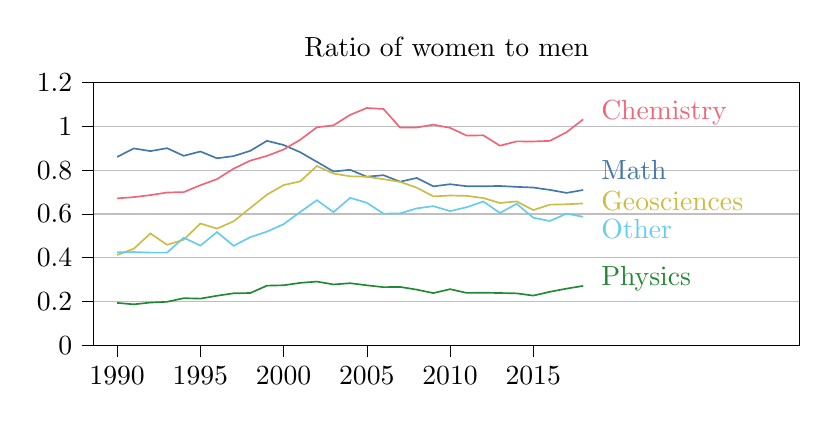
\begin{tikzpicture}

\definecolor{color0}{rgb}{0.266666666666667,0.466666666666667,0.666666666666667}
\definecolor{color1}{rgb}{0.933333333333333,0.4,0.466666666666667}
\definecolor{color2}{rgb}{0.133333333333333,0.533333333333333,0.2}
\definecolor{color3}{rgb}{0.8,0.733333333333333,0.266666666666667}
\definecolor{color4}{rgb}{0.4,0.8,0.933333333333333}

\begin{axis}[
height=140pt,
tick align=outside,
tick pos=left,
title={Ratio of women to men},
width=300pt,
x grid style={white!69.0196078431373!black},
xmin=1988.6, xmax=2031,
xtick style={color=black},
xtick={1990,1995,2000,2005,2010,2015},
xticklabels={\(\displaystyle 1990\),\(\displaystyle 1995\),\(\displaystyle 2000\),\(\displaystyle 2005\),\(\displaystyle 2010\),\(\displaystyle 2015\)},
ymajorgrids,
ymin=0, ymax=1.2,
ytick style={color=black},
ytick={0,0.2,0.4,0.6,0.8,1,1.2},
yticklabels={\(\displaystyle 0\),\(\displaystyle 0.2\),\(\displaystyle 0.4\),\(\displaystyle 0.6\),\(\displaystyle 0.8\),\(\displaystyle 1\),\(\displaystyle 1.2\)}
]
\addplot [semithick, color0]
table {%
1990 0.86025857925415
1991 0.899104356765747
1992 0.886856079101562
1993 0.900158047676086
1994 0.865336656570435
1995 0.88508152961731
1996 0.85411524772644
1997 0.864051580429077
1998 0.88809061050415
1999 0.93377161026001
2000 0.914776563644409
2001 0.881730198860168
2003 0.793915510177612
2004 0.801473140716553
2005 0.769950985908508
2006 0.776896238327026
2007 0.747289896011353
2008 0.764146089553833
2009 0.725896239280701
2010 0.73568868637085
2011 0.726636171340942
2012 0.726435899734497
2013 0.727647542953491
2014 0.723636150360107
2015 0.720515251159668
2016 0.709809184074402
2017 0.696071982383728
2018 0.709341764450073
};
\addplot [semithick, color1]
table {%
1990 0.671039342880249
1991 0.676785707473755
1992 0.685910940170288
1993 0.69794774055481
1994 0.69971776008606
1995 0.731048822402954
1996 0.759006500244141
1997 0.806735277175903
1998 0.843441247940063
1999 0.864903688430786
2000 0.894080996513367
2001 0.938588261604309
2002 0.995605230331421
2003 1.00445258617401
2004 1.05229568481445
2005 1.08357799053192
2006 1.0791380405426
2007 0.994340896606445
2008 0.994724988937378
2009 1.00745689868927
2010 0.993175625801086
2011 0.957595586776733
2012 0.958948135375977
2013 0.91149640083313
2014 0.931159019470215
2015 0.93084180355072
2016 0.933491468429565
2017 0.97307550907135
2018 1.03163325786591
};
\addplot [semithick, color2]
table {%
1990 0.194038391113281
1991 0.187412619590759
1992 0.195633172988892
1993 0.198942065238953
1994 0.21547794342041
1995 0.213540077209473
1996 0.22656512260437
1997 0.237869381904602
1998 0.239068150520325
1999 0.272727251052856
2000 0.274450302124023
2001 0.285370826721191
2002 0.291399240493774
2003 0.278211355209351
2004 0.283905506134033
2005 0.274263858795166
2006 0.265949487686157
2007 0.266808748245239
2008 0.254617691040039
2009 0.238819718360901
2010 0.256713628768921
2011 0.239596724510193
2012 0.240569829940796
2014 0.237533092498779
2015 0.227295517921448
2016 0.244655251502991
2017 0.259088039398193
2018 0.271610617637634
};
\addplot [semithick, color3]
table {%
1990 0.412641644477844
1991 0.441265940666199
1992 0.510834217071533
1993 0.459031701087952
1994 0.482448577880859
1995 0.556327104568481
1996 0.53315544128418
1997 0.566381931304932
1999 0.687969923019409
2000 0.731742858886719
2001 0.748560428619385
2002 0.818825960159302
2003 0.7843337059021
2004 0.771822333335876
2005 0.769706249237061
2006 0.758743047714233
2007 0.746450304985046
2008 0.720018625259399
2009 0.680118918418884
2010 0.684106230735779
2011 0.682439565658569
2012 0.672641515731812
2013 0.649957060813904
2014 0.657241940498352
2015 0.617704272270203
2016 0.642288208007812
2017 0.644059658050537
2018 0.64803409576416
};
\addplot [semithick, color4]
table {%
1990 0.4248366355896
1991 0.426124215126038
1992 0.423603773117065
1993 0.423517227172852
1994 0.491578936576843
1995 0.455523014068604
1996 0.517167329788208
1997 0.454545497894287
1998 0.49407958984375
1999 0.519343495368958
2000 0.553086400032043
2001 0.608958840370178
2002 0.662933945655823
2003 0.608324527740479
2004 0.673349142074585
2005 0.651209592819214
2006 0.601332068443298
2007 0.602455139160156
2008 0.625346899032593
2009 0.635593175888062
2010 0.612959742546082
2011 0.630742073059082
2012 0.656804800033569
2013 0.604386687278748
2014 0.646360754966736
2015 0.582999229431152
2016 0.567901253700256
2017 0.60113263130188
2018 0.58702540397644
};
\draw (axis cs:2018.5,0.759341764874964) node[
  anchor=base west,
  text=color0,
  rotate=0.0
]{Math};
\draw (axis cs:2018.5,1.03163331181407) node[
  anchor=base west,
  text=color1,
  rotate=0.0
]{Chemistry};
\draw (axis cs:2018.5,0.271610624904038) node[
  anchor=base west,
  text=color2,
  rotate=0.0
]{Physics};
\draw (axis cs:2018.5,0.618034107058266) node[
  anchor=base west,
  text=color3,
  rotate=0.0
]{Geosciences};
\draw (axis cs:2018.5,0.487025316455696) node[
  anchor=base west,
  text=color4,
  rotate=0.0
]{Other};
\end{axis}

\end{tikzpicture}

\vspace{0.1cm}
\begin{tikzpicture}
% This file was created by tikzplotlib v0.9.2.
\definecolor{color0}{rgb}{0.266666666666667,0.466666666666667,0.666666666666667}
\definecolor{color1}{rgb}{0.933333333333333,0.4,0.466666666666667}
\definecolor{color2}{rgb}{0.133333333333333,0.533333333333333,0.2}
\definecolor{color3}{rgb}{0.8,0.733333333333333,0.266666666666667}
\definecolor{color4}{rgb}{0.4,0.8,0.933333333333333}

\begin{groupplot}[group style={group size=2 by 1, group name=my plots, horizontal sep=0.8cm}]
\nextgroupplot[
height=90pt, width=160pt,
legend style={at={(2.02, 0.5)},anchor=west,},
reverse legend,
tick align=outside,
tick pos=left,
x grid style={white!69.0196078431373!black},
xlabel={Women},
xmin=1988.6, xmax=2019.4,
xtick style={color=black},
xtick={1990,2000,2010},
xticklabels={\(\displaystyle 1990\),\(\displaystyle 2000\),\(\displaystyle 2010\)},
ymajorgrids,
ymin=0, ymax=26.8548,
ytick style={color=black}
]
\path [draw=color0, fill=color0]
(axis cs:1990,6.587)
--(axis cs:1990,0)
--(axis cs:1991,0)
--(axis cs:1992,0)
--(axis cs:1993,0)
--(axis cs:1994,0)
--(axis cs:1995,0)
--(axis cs:1996,0)
--(axis cs:1997,0)
--(axis cs:1998,0)
--(axis cs:1999,0)
--(axis cs:2000,0)
--(axis cs:2001,0)
--(axis cs:2002,0)
--(axis cs:2003,0)
--(axis cs:2004,0)
--(axis cs:2005,0)
--(axis cs:2006,0)
--(axis cs:2007,0)
--(axis cs:2008,0)
--(axis cs:2009,0)
--(axis cs:2010,0)
--(axis cs:2011,0)
--(axis cs:2012,0)
--(axis cs:2013,0)
--(axis cs:2014,0)
--(axis cs:2015,0)
--(axis cs:2016,0)
--(axis cs:2017,0)
--(axis cs:2018,0)
--(axis cs:2018,12.339)
--(axis cs:2018,12.339)
--(axis cs:2017,11.607)
--(axis cs:2016,11.122)
--(axis cs:2015,10.74)
--(axis cs:2014,10.293)
--(axis cs:2013,10.059)
--(axis cs:2012,9.233)
--(axis cs:2011,8.405)
--(axis cs:2010,7.788)
--(axis cs:2009,7.431)
--(axis cs:2008,7.468)
--(axis cs:2007,7.307)
--(axis cs:2006,7.344)
--(axis cs:2005,7.072)
--(axis cs:2004,6.746)
--(axis cs:2003,6.237)
--(axis cs:2002,6.085)
--(axis cs:2001,5.83)
--(axis cs:2000,5.485)
--(axis cs:1999,5.823)
--(axis cs:1998,5.563)
--(axis cs:1997,5.771)
--(axis cs:1996,5.884)
--(axis cs:1995,6.354)
--(axis cs:1994,6.593)
--(axis cs:1993,6.834)
--(axis cs:1992,6.835)
--(axis cs:1991,6.826)
--(axis cs:1990,6.587)
--cycle;

\path [draw=color1, fill=color1]
(axis cs:1990,9.912)
--(axis cs:1990,6.587)
--(axis cs:1991,6.826)
--(axis cs:1992,6.835)
--(axis cs:1993,6.834)
--(axis cs:1994,6.593)
--(axis cs:1995,6.354)
--(axis cs:1996,5.884)
--(axis cs:1997,5.771)
--(axis cs:1998,5.563)
--(axis cs:1999,5.823)
--(axis cs:2000,5.485)
--(axis cs:2001,5.83)
--(axis cs:2002,6.085)
--(axis cs:2003,6.237)
--(axis cs:2004,6.746)
--(axis cs:2005,7.072)
--(axis cs:2006,7.344)
--(axis cs:2007,7.307)
--(axis cs:2008,7.468)
--(axis cs:2009,7.431)
--(axis cs:2010,7.788)
--(axis cs:2011,8.405)
--(axis cs:2012,9.233)
--(axis cs:2013,10.059)
--(axis cs:2014,10.293)
--(axis cs:2015,10.74)
--(axis cs:2016,11.122)
--(axis cs:2017,11.607)
--(axis cs:2018,12.339)
--(axis cs:2018,20.329)
--(axis cs:2018,20.329)
--(axis cs:2017,19.558)
--(axis cs:2016,18.603)
--(axis cs:2015,18.237)
--(axis cs:2014,17.773)
--(axis cs:2013,17.155)
--(axis cs:2012,16.381)
--(axis cs:2011,15.112)
--(axis cs:2010,14.337)
--(axis cs:2009,13.916)
--(axis cs:2008,13.691)
--(axis cs:2007,13.281)
--(axis cs:2006,13.303)
--(axis cs:2005,12.608)
--(axis cs:2004,11.857)
--(axis cs:2003,11.2)
--(axis cs:2002,11.069)
--(axis cs:2001,10.843)
--(axis cs:2000,10.364)
--(axis cs:1999,10.631)
--(axis cs:1998,10.514)
--(axis cs:1997,10.634)
--(axis cs:1996,10.498)
--(axis cs:1995,10.578)
--(axis cs:1994,10.559)
--(axis cs:1993,10.575)
--(axis cs:1992,10.423)
--(axis cs:1991,10.237)
--(axis cs:1990,9.912)
--cycle;

\path [draw=color2, fill=color2]
(axis cs:1990,10.589)
--(axis cs:1990,9.912)
--(axis cs:1991,10.237)
--(axis cs:1992,10.423)
--(axis cs:1993,10.575)
--(axis cs:1994,10.559)
--(axis cs:1995,10.578)
--(axis cs:1996,10.498)
--(axis cs:1997,10.634)
--(axis cs:1998,10.514)
--(axis cs:1999,10.631)
--(axis cs:2000,10.364)
--(axis cs:2001,10.843)
--(axis cs:2002,11.069)
--(axis cs:2003,11.2)
--(axis cs:2004,11.857)
--(axis cs:2005,12.608)
--(axis cs:2006,13.303)
--(axis cs:2007,13.281)
--(axis cs:2008,13.691)
--(axis cs:2009,13.916)
--(axis cs:2010,14.337)
--(axis cs:2011,15.112)
--(axis cs:2012,16.381)
--(axis cs:2013,17.155)
--(axis cs:2014,17.773)
--(axis cs:2015,18.237)
--(axis cs:2016,18.603)
--(axis cs:2017,19.558)
--(axis cs:2018,20.329)
--(axis cs:2018,22.098)
--(axis cs:2018,22.098)
--(axis cs:2017,21.183)
--(axis cs:2016,20.125)
--(axis cs:2015,19.596)
--(axis cs:2014,19.121)
--(axis cs:2013,18.462)
--(axis cs:2012,17.58)
--(axis cs:2011,16.229)
--(axis cs:2010,15.465)
--(axis cs:2009,14.952)
--(axis cs:2008,14.78)
--(axis cs:2007,14.408)
--(axis cs:2006,14.366)
--(axis cs:2005,13.614)
--(axis cs:2004,12.866)
--(axis cs:2003,12.127)
--(axis cs:2002,11.977)
--(axis cs:2001,11.674)
--(axis cs:2000,11.088)
--(axis cs:1999,11.324)
--(axis cs:1998,11.181)
--(axis cs:1997,11.286)
--(axis cs:1996,11.182)
--(axis cs:1995,11.253)
--(axis cs:1994,11.269)
--(axis cs:1993,11.252)
--(axis cs:1992,11.095)
--(axis cs:1991,10.907)
--(axis cs:1990,10.589)
--cycle;

\path [draw=color3, fill=color3]
(axis cs:1990,11.281)
--(axis cs:1990,10.589)
--(axis cs:1991,10.907)
--(axis cs:1992,11.095)
--(axis cs:1993,11.252)
--(axis cs:1994,11.269)
--(axis cs:1995,11.253)
--(axis cs:1996,11.182)
--(axis cs:1997,11.286)
--(axis cs:1998,11.181)
--(axis cs:1999,11.324)
--(axis cs:2000,11.088)
--(axis cs:2001,11.674)
--(axis cs:2002,11.977)
--(axis cs:2003,12.127)
--(axis cs:2004,12.866)
--(axis cs:2005,13.614)
--(axis cs:2006,14.366)
--(axis cs:2007,14.408)
--(axis cs:2008,14.78)
--(axis cs:2009,14.952)
--(axis cs:2010,15.465)
--(axis cs:2011,16.229)
--(axis cs:2012,17.58)
--(axis cs:2013,18.462)
--(axis cs:2014,19.121)
--(axis cs:2015,19.596)
--(axis cs:2016,20.125)
--(axis cs:2017,21.183)
--(axis cs:2018,22.098)
--(axis cs:2018,24.834)
--(axis cs:2018,24.834)
--(axis cs:2017,23.861)
--(axis cs:2016,22.786)
--(axis cs:2015,22.136)
--(axis cs:2014,21.585)
--(axis cs:2013,20.731)
--(axis cs:2012,19.719)
--(axis cs:2011,18.176)
--(axis cs:2010,17.191)
--(axis cs:2009,16.553)
--(axis cs:2008,16.323)
--(axis cs:2007,15.88)
--(axis cs:2006,15.863)
--(axis cs:2005,15.108)
--(axis cs:2004,14.378)
--(axis cs:2003,13.669)
--(axis cs:2002,13.595)
--(axis cs:2001,13.234)
--(axis cs:2000,12.591)
--(axis cs:1999,12.788)
--(axis cs:1998,12.676)
--(axis cs:1997,12.745)
--(axis cs:1996,12.581)
--(axis cs:1995,12.695)
--(axis cs:1994,12.396)
--(axis cs:1993,12.238)
--(axis cs:1992,12.038)
--(axis cs:1991,11.632)
--(axis cs:1990,11.281)
--cycle;

\path [draw=color4, fill=color4]
(axis cs:1990,11.671)
--(axis cs:1990,11.281)
--(axis cs:1991,11.632)
--(axis cs:1992,12.038)
--(axis cs:1993,12.238)
--(axis cs:1994,12.396)
--(axis cs:1995,12.695)
--(axis cs:1996,12.581)
--(axis cs:1997,12.745)
--(axis cs:1998,12.676)
--(axis cs:1999,12.788)
--(axis cs:2000,12.591)
--(axis cs:2001,13.234)
--(axis cs:2002,13.595)
--(axis cs:2003,13.669)
--(axis cs:2004,14.378)
--(axis cs:2005,15.108)
--(axis cs:2006,15.863)
--(axis cs:2007,15.88)
--(axis cs:2008,16.323)
--(axis cs:2009,16.553)
--(axis cs:2010,17.191)
--(axis cs:2011,18.176)
--(axis cs:2012,19.719)
--(axis cs:2013,20.731)
--(axis cs:2014,21.585)
--(axis cs:2015,22.136)
--(axis cs:2016,22.786)
--(axis cs:2017,23.861)
--(axis cs:2018,24.834)
--(axis cs:2018,25.576)
--(axis cs:2018,25.576)
--(axis cs:2017,24.604)
--(axis cs:2016,23.476)
--(axis cs:2015,22.863)
--(axis cs:2014,22.402)
--(axis cs:2013,21.475)
--(axis cs:2012,20.496)
--(axis cs:2011,18.89)
--(axis cs:2010,17.891)
--(axis cs:2009,17.228)
--(axis cs:2008,16.999)
--(axis cs:2007,16.518)
--(axis cs:2006,16.495)
--(axis cs:2005,15.754)
--(axis cs:2004,14.949)
--(axis cs:2003,14.239)
--(axis cs:2002,14.187)
--(axis cs:2001,13.737)
--(axis cs:2000,13.039)
--(axis cs:1999,13.231)
--(axis cs:1998,13.135)
--(axis cs:1997,13.175)
--(axis cs:1996,13.063)
--(axis cs:1995,13.161)
--(axis cs:1994,12.863)
--(axis cs:1993,12.645)
--(axis cs:1992,12.44)
--(axis cs:1991,12.03)
--(axis cs:1990,11.671)
--cycle;

\addplot [semithick, color0]
table {%
1990 6.58699989318848
1991 6.82600021362305
1992 6.83500003814697
1993 6.83400011062622
1995 6.35400009155273
1996 5.88399982452393
1997 5.77099990844727
1998 5.56300020217896
1999 5.82299995422363
2000 5.4850001335144
2001 5.82999992370605
2002 6.08500003814697
2003 6.23699998855591
2004 6.74599981307983
2005 7.07200002670288
2006 7.3439998626709
2007 7.30700016021729
2008 7.46799993515015
2009 7.43100023269653
2010 7.78800010681152
2011 8.40499973297119
2013 10.0590000152588
2014 10.2930002212524
2015 10.7399997711182
2016 11.1219997406006
2017 11.6070003509521
2018 12.33899974823
};
\addplot [semithick, color1]
table {%
1990 9.91199970245361
1991 10.2370004653931
1992 10.4230003356934
1993 10.5749998092651
1994 10.5590000152588
1995 10.5780000686646
1996 10.4980001449585
1997 10.6339998245239
1998 10.5139999389648
1999 10.6309995651245
2000 10.3640003204346
2001 10.8430004119873
2002 11.0690002441406
2003 11.1999998092651
2004 11.8570003509521
2005 12.6079998016357
2006 13.3030004501343
2007 13.2810001373291
2008 13.6909999847412
2009 13.9160003662109
2010 14.3369998931885
2011 15.1120004653931
2012 16.3810005187988
2013 17.1550006866455
2014 17.7730007171631
2015 18.2369995117188
2016 18.6030006408691
2017 19.5580005645752
2018 20.3290004730225
};
\addplot [semithick, color2]
table {%
1990 10.58899974823
1991 10.9069995880127
1992 11.0950002670288
1993 11.2519998550415
1994 11.2690000534058
1995 11.2530002593994
1996 11.1820001602173
1997 11.28600025177
1998 11.1809997558594
1999 11.3240003585815
2000 11.0880002975464
2001 11.673999786377
2002 11.9770002365112
2003 12.1269998550415
2005 13.6140003204346
2006 14.3660001754761
2007 14.4079999923706
2008 14.7799997329712
2009 14.9519996643066
2010 15.4650001525879
2011 16.2290000915527
2012 17.5799999237061
2013 18.4619998931885
2014 19.121000289917
2015 19.5960006713867
2016 20.125
2017 21.1830005645752
2018 22.0979995727539
};
\addplot [semithick, color3]
table {%
1990 11.2810001373291
1991 11.6319999694824
1992 12.0380001068115
1993 12.2379999160767
1994 12.3959999084473
1995 12.6949996948242
1996 12.581000328064
1997 12.7449998855591
1998 12.6759996414185
1999 12.7880001068115
2000 12.5909996032715
2001 13.2340002059937
2002 13.5950002670288
2003 13.668999671936
2004 14.3780002593994
2005 15.1079998016357
2006 15.8629999160767
2007 15.8800001144409
2008 16.3229999542236
2009 16.55299949646
2010 17.1909999847412
2011 18.1760005950928
2012 19.7189998626709
2013 20.7310009002686
2014 21.5849990844727
2015 22.1359996795654
2016 22.7859992980957
2017 23.8610000610352
2018 24.8339996337891
};
\addplot [semithick, color4]
table {%
1990 11.6709995269775
1991 12.0299997329712
1992 12.4399995803833
1993 12.6450004577637
1994 12.8629999160767
1995 13.16100025177
1996 13.0629997253418
1997 13.1750001907349
1998 13.1350002288818
1999 13.2309999465942
2000 13.0389995574951
2001 13.7370004653931
2002 14.1870002746582
2003 14.2390003204346
2004 14.9490003585815
2005 15.753999710083
2006 16.4950008392334
2007 16.5179996490479
2008 16.9990005493164
2009 17.2280006408691
2010 17.8910007476807
2011 18.8899993896484
2012 20.496000289917
2013 21.4750003814697
2014 22.4020004272461
2015 22.863000869751
2016 23.4759998321533
2017 24.6040000915527
2018 25.576000213623
};

\nextgroupplot[
height=90pt, width=160pt,
legend style={at={(2.02, 0.5)},anchor=west,},
reverse legend,
tick align=outside,
tick pos=left,
x grid style={white!69.0196078431373!black},
xlabel={Men},
xmin=1988.6, xmax=2019.4,
xtick style={color=black},
xtick={1990,2000,2010},
xticklabels={\(\displaystyle 1990\),\(\displaystyle 2000\),\(\displaystyle 2010\)},
ymajorgrids,
ymin=0, ymax=38.99595,
ytick style={color=black}
]
\path [draw=color0, fill=color0]
(axis cs:1990,7.657)
--(axis cs:1990,0)
--(axis cs:1991,0)
--(axis cs:1992,0)
--(axis cs:1993,0)
--(axis cs:1994,0)
--(axis cs:1995,0)
--(axis cs:1996,0)
--(axis cs:1997,0)
--(axis cs:1998,0)
--(axis cs:1999,0)
--(axis cs:2000,0)
--(axis cs:2001,0)
--(axis cs:2002,0)
--(axis cs:2003,0)
--(axis cs:2004,0)
--(axis cs:2005,0)
--(axis cs:2006,0)
--(axis cs:2007,0)
--(axis cs:2008,0)
--(axis cs:2009,0)
--(axis cs:2010,0)
--(axis cs:2011,0)
--(axis cs:2012,0)
--(axis cs:2013,0)
--(axis cs:2014,0)
--(axis cs:2015,0)
--(axis cs:2016,0)
--(axis cs:2017,0)
--(axis cs:2018,0)
--(axis cs:2018,17.395)
--(axis cs:2018,17.395)
--(axis cs:2017,16.675)
--(axis cs:2016,15.669)
--(axis cs:2015,14.906)
--(axis cs:2014,14.224)
--(axis cs:2013,13.824)
--(axis cs:2012,12.71)
--(axis cs:2011,11.567)
--(axis cs:2010,10.586)
--(axis cs:2009,10.237)
--(axis cs:2008,9.773)
--(axis cs:2007,9.778)
--(axis cs:2006,9.453)
--(axis cs:2005,9.185)
--(axis cs:2004,8.417)
--(axis cs:2003,7.856)
--(axis cs:2002,7.262)
--(axis cs:2001,6.612)
--(axis cs:2000,5.996)
--(axis cs:1999,6.236)
--(axis cs:1998,6.264)
--(axis cs:1997,6.679)
--(axis cs:1996,6.889)
--(axis cs:1995,7.179)
--(axis cs:1994,7.619)
--(axis cs:1993,7.592)
--(axis cs:1992,7.707)
--(axis cs:1991,7.592)
--(axis cs:1990,7.657)
--cycle;

\path [draw=color1, fill=color1]
(axis cs:1990,12.612)
--(axis cs:1990,7.657)
--(axis cs:1991,7.592)
--(axis cs:1992,7.707)
--(axis cs:1993,7.592)
--(axis cs:1994,7.619)
--(axis cs:1995,7.179)
--(axis cs:1996,6.889)
--(axis cs:1997,6.679)
--(axis cs:1998,6.264)
--(axis cs:1999,6.236)
--(axis cs:2000,5.996)
--(axis cs:2001,6.612)
--(axis cs:2002,7.262)
--(axis cs:2003,7.856)
--(axis cs:2004,8.417)
--(axis cs:2005,9.185)
--(axis cs:2006,9.453)
--(axis cs:2007,9.778)
--(axis cs:2008,9.773)
--(axis cs:2009,10.237)
--(axis cs:2010,10.586)
--(axis cs:2011,11.567)
--(axis cs:2012,12.71)
--(axis cs:2013,13.824)
--(axis cs:2014,14.224)
--(axis cs:2015,14.906)
--(axis cs:2016,15.669)
--(axis cs:2017,16.675)
--(axis cs:2018,17.395)
--(axis cs:2018,25.14)
--(axis cs:2018,25.14)
--(axis cs:2017,24.846)
--(axis cs:2016,23.683)
--(axis cs:2015,22.96)
--(axis cs:2014,22.257)
--(axis cs:2013,21.609)
--(axis cs:2012,20.164)
--(axis cs:2011,18.571)
--(axis cs:2010,17.18)
--(axis cs:2009,16.674)
--(axis cs:2008,16.029)
--(axis cs:2007,15.786)
--(axis cs:2006,14.975)
--(axis cs:2005,14.294)
--(axis cs:2004,13.274)
--(axis cs:2003,12.797)
--(axis cs:2002,12.268)
--(axis cs:2001,11.953)
--(axis cs:2000,11.453)
--(axis cs:1999,11.795)
--(axis cs:1998,12.134)
--(axis cs:1997,12.707)
--(axis cs:1996,12.968)
--(axis cs:1995,12.957)
--(axis cs:1994,13.287)
--(axis cs:1993,12.952)
--(axis cs:1992,12.938)
--(axis cs:1991,12.632)
--(axis cs:1990,12.612)
--cycle;

\path [draw=color2, fill=color2]
(axis cs:1990,16.101)
--(axis cs:1990,12.612)
--(axis cs:1991,12.632)
--(axis cs:1992,12.938)
--(axis cs:1993,12.952)
--(axis cs:1994,13.287)
--(axis cs:1995,12.957)
--(axis cs:1996,12.968)
--(axis cs:1997,12.707)
--(axis cs:1998,12.134)
--(axis cs:1999,11.795)
--(axis cs:2000,11.453)
--(axis cs:2001,11.953)
--(axis cs:2002,12.268)
--(axis cs:2003,12.797)
--(axis cs:2004,13.274)
--(axis cs:2005,14.294)
--(axis cs:2006,14.975)
--(axis cs:2007,15.786)
--(axis cs:2008,16.029)
--(axis cs:2009,16.674)
--(axis cs:2010,17.18)
--(axis cs:2011,18.571)
--(axis cs:2012,20.164)
--(axis cs:2013,21.609)
--(axis cs:2014,22.257)
--(axis cs:2015,22.96)
--(axis cs:2016,23.683)
--(axis cs:2017,24.846)
--(axis cs:2018,25.14)
--(axis cs:2018,31.653)
--(axis cs:2018,31.653)
--(axis cs:2017,31.118)
--(axis cs:2016,29.904)
--(axis cs:2015,28.939)
--(axis cs:2014,27.932)
--(axis cs:2013,27.072)
--(axis cs:2012,25.148)
--(axis cs:2011,23.233)
--(axis cs:2010,21.574)
--(axis cs:2009,21.012)
--(axis cs:2008,20.306)
--(axis cs:2007,20.01)
--(axis cs:2006,18.972)
--(axis cs:2005,17.962)
--(axis cs:2004,16.828)
--(axis cs:2003,16.129)
--(axis cs:2002,15.384)
--(axis cs:2001,14.865)
--(axis cs:2000,14.091)
--(axis cs:1999,14.336)
--(axis cs:1998,14.924)
--(axis cs:1997,15.448)
--(axis cs:1996,15.987)
--(axis cs:1995,16.118)
--(axis cs:1994,16.582)
--(axis cs:1993,16.355)
--(axis cs:1992,16.373)
--(axis cs:1991,16.207)
--(axis cs:1990,16.101)
--cycle;

\path [draw=color3, fill=color3]
(axis cs:1990,17.778)
--(axis cs:1990,16.101)
--(axis cs:1991,16.207)
--(axis cs:1992,16.373)
--(axis cs:1993,16.355)
--(axis cs:1994,16.582)
--(axis cs:1995,16.118)
--(axis cs:1996,15.987)
--(axis cs:1997,15.448)
--(axis cs:1998,14.924)
--(axis cs:1999,14.336)
--(axis cs:2000,14.091)
--(axis cs:2001,14.865)
--(axis cs:2002,15.384)
--(axis cs:2003,16.129)
--(axis cs:2004,16.828)
--(axis cs:2005,17.962)
--(axis cs:2006,18.972)
--(axis cs:2007,20.01)
--(axis cs:2008,20.306)
--(axis cs:2009,21.012)
--(axis cs:2010,21.574)
--(axis cs:2011,23.233)
--(axis cs:2012,25.148)
--(axis cs:2013,27.072)
--(axis cs:2014,27.932)
--(axis cs:2015,28.939)
--(axis cs:2016,29.904)
--(axis cs:2017,31.118)
--(axis cs:2018,31.653)
--(axis cs:2018,35.875)
--(axis cs:2018,35.875)
--(axis cs:2017,35.276)
--(axis cs:2016,34.047)
--(axis cs:2015,33.051)
--(axis cs:2014,31.681)
--(axis cs:2013,30.563)
--(axis cs:2012,28.328)
--(axis cs:2011,26.086)
--(axis cs:2010,24.097)
--(axis cs:2009,23.366)
--(axis cs:2008,22.449)
--(axis cs:2007,21.982)
--(axis cs:2006,20.945)
--(axis cs:2005,19.903)
--(axis cs:2004,18.787)
--(axis cs:2003,18.095)
--(axis cs:2002,17.36)
--(axis cs:2001,16.949)
--(axis cs:2000,16.145)
--(axis cs:1999,16.464)
--(axis cs:1998,17.307)
--(axis cs:1997,18.024)
--(axis cs:1996,18.611)
--(axis cs:1995,18.71)
--(axis cs:1994,18.918)
--(axis cs:1993,18.503)
--(axis cs:1992,18.219)
--(axis cs:1991,17.85)
--(axis cs:1990,17.778)
--cycle;

\path [draw=color4, fill=color4]
(axis cs:1990,18.696)
--(axis cs:1990,17.778)
--(axis cs:1991,17.85)
--(axis cs:1992,18.219)
--(axis cs:1993,18.503)
--(axis cs:1994,18.918)
--(axis cs:1995,18.71)
--(axis cs:1996,18.611)
--(axis cs:1997,18.024)
--(axis cs:1998,17.307)
--(axis cs:1999,16.464)
--(axis cs:2000,16.145)
--(axis cs:2001,16.949)
--(axis cs:2002,17.36)
--(axis cs:2003,18.095)
--(axis cs:2004,18.787)
--(axis cs:2005,19.903)
--(axis cs:2006,20.945)
--(axis cs:2007,21.982)
--(axis cs:2008,22.449)
--(axis cs:2009,23.366)
--(axis cs:2010,24.097)
--(axis cs:2011,26.086)
--(axis cs:2012,28.328)
--(axis cs:2013,30.563)
--(axis cs:2014,31.681)
--(axis cs:2015,33.051)
--(axis cs:2016,34.047)
--(axis cs:2017,35.276)
--(axis cs:2018,35.875)
--(axis cs:2018,37.139)
--(axis cs:2018,37.139)
--(axis cs:2017,36.512)
--(axis cs:2016,35.262)
--(axis cs:2015,34.298)
--(axis cs:2014,32.945)
--(axis cs:2013,31.794)
--(axis cs:2012,29.511)
--(axis cs:2011,27.218)
--(axis cs:2010,25.239)
--(axis cs:2009,24.428)
--(axis cs:2008,23.53)
--(axis cs:2007,23.041)
--(axis cs:2006,21.996)
--(axis cs:2005,20.895)
--(axis cs:2004,19.635)
--(axis cs:2003,19.032)
--(axis cs:2002,18.253)
--(axis cs:2001,17.775)
--(axis cs:2000,16.955)
--(axis cs:1999,17.317)
--(axis cs:1998,18.236)
--(axis cs:1997,18.97)
--(axis cs:1996,19.543)
--(axis cs:1995,19.733)
--(axis cs:1994,19.868)
--(axis cs:1993,19.464)
--(axis cs:1992,19.168)
--(axis cs:1991,18.784)
--(axis cs:1990,18.696)
--cycle;

\addplot [semithick, color0]
table {%
1990 7.65700006484985
1991 7.59200000762939
1992 7.70699977874756
1993 7.59200000762939
1994 7.61899995803833
1995 7.17899990081787
1996 6.88899993896484
1997 6.67899990081787
1998 6.26399993896484
1999 6.23600006103516
2000 5.99599981307983
2001 6.61199998855591
2002 7.26200008392334
2003 7.85599994659424
2004 8.41699981689453
2005 9.1850004196167
2006 9.45300006866455
2007 9.77799987792969
2008 9.77299976348877
2009 10.2370004653931
2010 10.5860004425049
2011 11.5670003890991
2012 12.710000038147
2013 13.8240003585815
2014 14.2239999771118
2015 14.9060001373291
2016 15.668999671936
2017 16.6749992370605
2018 17.3950004577637
};
\addplot [semithick, color1]
table {%
1990 12.6120004653931
1991 12.6319999694824
1992 12.9379997253418
1993 12.9519996643066
1994 13.2869997024536
1995 12.9569997787476
1996 12.9680004119873
1997 12.7069997787476
1998 12.1339998245239
2000 11.4530000686646
2001 11.9530000686646
2002 12.2679996490479
2003 12.7969999313354
2004 13.2740001678467
2005 14.293999671936
2006 14.9750003814697
2007 15.78600025177
2008 16.0289993286133
2009 16.673999786377
2010 17.1800003051758
2011 18.5709991455078
2012 20.1639995574951
2013 21.6089992523193
2014 22.2569999694824
2015 22.9599990844727
2016 23.6830005645752
2017 24.8460006713867
2018 25.1399993896484
};
\addplot [semithick, color2]
table {%
1990 16.1009998321533
1991 16.2070007324219
1992 16.3729991912842
1993 16.3549995422363
1994 16.5820007324219
1995 16.1180000305176
1996 15.9870004653931
1997 15.4479999542236
1998 14.923999786377
1999 14.3360004425049
2000 14.0909996032715
2001 14.8649997711182
2002 15.3839998245239
2003 16.128999710083
2004 16.8279991149902
2005 17.9619998931885
2006 18.9720001220703
2007 20.0100002288818
2008 20.3059997558594
2009 21.011999130249
2010 21.5739994049072
2011 23.2329998016357
2013 27.07200050354
2014 27.931999206543
2015 28.9389991760254
2016 29.9039993286133
2017 31.1180000305176
2018 31.6529998779297
};
\addplot [semithick, color3]
table {%
1990 17.7779998779297
1991 17.8500003814697
1992 18.2189998626709
1993 18.5030002593994
1994 18.9179992675781
1995 18.7099990844727
1996 18.6110000610352
1997 18.0240001678467
1998 17.306999206543
1999 16.4640007019043
2000 16.1450004577637
2001 16.9489994049072
2002 17.3600006103516
2003 18.0949993133545
2004 18.7870006561279
2005 19.9029998779297
2007 21.9820003509521
2008 22.4489994049072
2009 23.3659992218018
2010 24.0970001220703
2011 26.0860004425049
2013 30.5629997253418
2014 31.6809997558594
2015 33.0509986877441
2016 34.0470008850098
2017 35.2760009765625
2018 35.875
};
\addplot [semithick, color4]
table {%
1990 18.6959991455078
1991 18.7840003967285
1992 19.1679992675781
1993 19.4640007019043
1994 19.8680000305176
1995 19.7329998016357
1996 19.5429992675781
1997 18.9699993133545
1998 18.2360000610352
1999 17.3169994354248
2000 16.9549999237061
2001 17.7749996185303
2002 18.2530002593994
2003 19.0319995880127
2004 19.6350002288818
2005 20.8950004577637
2006 21.996000289917
2007 23.0410003662109
2008 23.5300006866455
2009 24.42799949646
2010 25.2390003204346
2011 27.2180004119873
2013 31.7940006256104
2014 32.9449996948242
2015 34.2980003356934
2016 35.2620010375977
2017 36.5120010375977
2018 37.1389999389648
};
\end{groupplot}



\draw ($(my plots c1r1.north)!0.5!(my plots c2r1.north) + (0, 0.25cm)$) node {Number Bachelor's degrees awarded (thousands)};
\end{tikzpicture}
\caption{Source: IPEDS}

\end{figure}
\hyperlink{app_science_math}{\beamerbutton{Return: Science and math}}
\hyperlink{intro_social_science_ratio}{\beamerbutton{Return: Social science ratio}}
}
\end{frame}

%%%%%%%%%%%%%%%%%%%%%%%%%%
% Appendix - Simulations %
%%%%%%%%%%%%%%%%%%%%%%%%%%

%%%%%%%%%%%%%%%%%%%%%%%%%%%%%%%%%%%%%%%%%%%%%%%%%%%%%%%%%%%%%%%%%%%%%%%%%%%%%%%%
\begin{frame}{Parametric example}\label{sim_parameterization}

% Monotonicity of stopping problem (ensured by $h_{j0} \leq \nu \alpha_{j0}$) 
% \begin{itemize}
%     \item [$\implies$] Optimality of one-step-look-ahead, i.e. comparing
%     \begin{enumerate}
%         \item Value of entering labor market as skill $j$ specialist today, to
%         \item Value of entering labor market as a skill $j$ specialist tomorrow
%     \end{enumerate}
% \end{itemize}
Assuming $h_{j0} = \nu \alpha_{j0}$ and letting $c_{jt}$ be time spent studying $j$:
\begin{itemize}
    \item [$\implies$] Deterministic stopping function
\end{itemize}
\begin{equation*}
    \frac{1- \delta}{\delta} \geq \frac{1}{c_{jt} + \alpha_{j0} + \beta_{j0}} \implies 
    c_j^* = \left\lceil \frac{\delta}{1 - \delta} \right\rceil - (\alpha_{j0} + \beta_{j0})
\end{equation*}
Graduation regions given by:
\begin{equation*}
    \mathcal{G}_j (\alpha_{jt}, \beta_{jt}) = \left\{ 
        \alpha_{jt}, \beta_{jt} 
        \left\vert \frac{\delta}{1 - \delta} \leq \alpha_{jt} + \beta_{jt}
    \right.\right\}
\end{equation*}

In this example, note that $\mathcal{G}_Y = \mathcal{G}_X$. Index in the graduation region given by $\frac{h_{jt}}{1 - \delta}$. Index when not in graduation region given by Binomial distribution with parameters $\left(c_j^* - c_j, \frac{h_{jt}}{\nu(c_{jt} + \alpha_{j0} + \beta{j0})}\right)$:
    % \mathcal{I}_j (\alpha_{jt}, \beta_{jt}) = 
    % \begin{cases}
    %     \frac{w_{jt}}{1 - \delta} h_{jt} &\text{ if } 
    %         \{\alpha_{jt}, \beta_{jt}\} \in \mathcal{G}_j \\ 
    %     \frac{w_{jt}}{1 - \delta} 
    %         \left(h_{jt} + \nu \mathbb{E}[\theta_j \vert \alpha_{jt}, \beta_{jt}]\right) &\text{ if } \{\alpha_{jt}, \beta_{jt}\} \notin \mathcal{G}_j
    % \end{cases}
\begin{align*}
\mathcal{I}_{jt} (h_{jt}, \alpha_{jt}, \beta_{jt}) = 
\begin{cases}
\frac{w_{jt} h_{jt}}{1 - \delta} & \text{if } \{\alpha_{jt}, \beta_{jt}\} \in \mathcal{G}_{j}, \\
\frac{w_{jt} h_{jt}}{1 - \delta} \sbr{
   \frac{
      \left\lceil \frac{\delta}{1 - \delta} \right\rceil
      \delta^{\left\lceil \frac{\delta}{1 - \delta} \right\rceil - c_{jt} - \alpha_{j0} - \beta_{j0}}}
   {c_{jt} + \alpha_{j0} + \beta_{j0}}
   } & \text{if } \{\alpha_{jt}, \beta_{jt}\} \notin \mathcal{G}_{j} \\
\end{cases}
\end{align*}

\hyperlink{simulate}{\beamergotobutton{Return: simulation set-up}}
\hyperlink{sim_beliefs}{\beamerbutton{Return: belief simulation}}
\hyperlink{id_model_notes}{\beamerbutton{Return: ID notes}}
\end{frame}


%%%%%%%%%%%%%%%%%%%%%%%%%%%%%%%%%%%%%%%%%%%%%%%%%%%%%%%%%%%%%%%%%%%%%%%%%%%%%%%%
\begin{frame}{}\label{app_ability_v_effect}

If 
$\nu_X = 
\frac{\alpha_{X0} + \beta_{X0}}{\alpha_{Y0} + \beta_{Y0}} 
\cdot \frac{\alpha_{Y0}}{\alpha_{X0}}
\cdot \delta^{\alpha_{X0} + \beta_{X0} - \alpha_{Y0} - \beta_{Y0}}$, then:
\begin{itemize}
     \item $h_{X0} = h_{Y0}$, and
     \item Agents randomly choose between fields $X$ and $Y$ at $t=0$
 \end{itemize}  
\begin{figure}
\centering
% This file was created by tikzplotlib v0.9.2.
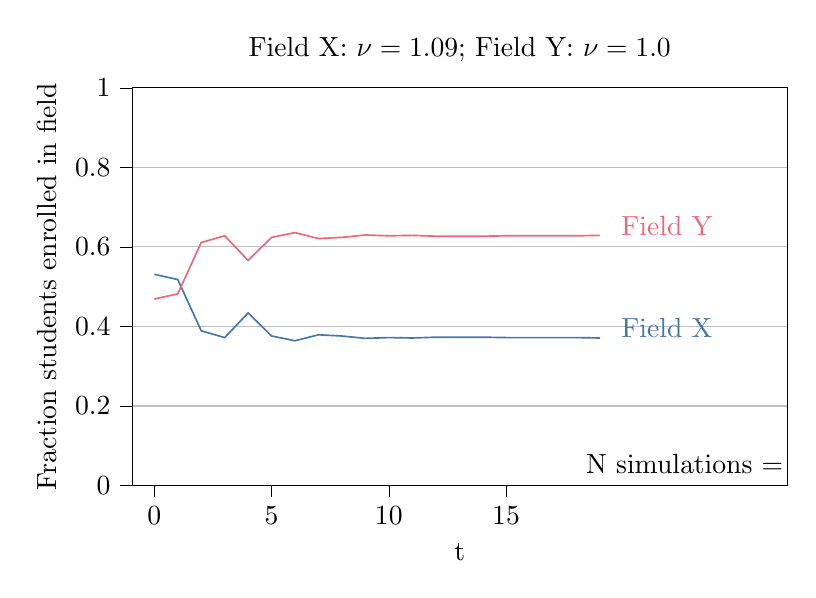
\begin{tikzpicture}

\definecolor{color0}{rgb}{0.266666666666667,0.466666666666667,0.666666666666667}
\definecolor{color1}{rgb}{0.933333333333333,0.4,0.466666666666667}

\begin{axis}[
height=6.6314113761540705cm,
tick align=outside,
tick pos=left,
title={Field X: \(\displaystyle \nu=1.09\); Field Y: \(\displaystyle \nu=1.0\)},
width=9.904475999999999cm,
x grid style={white!69.0196078431373!black},
xlabel={t},
xmin=-0.95, xmax=27,
xtick style={color=black},
xtick={0,5,10,15},
xticklabels={\(\displaystyle 0\),\(\displaystyle 5\),\(\displaystyle 10\),\(\displaystyle 15\)},
ylabel={Fraction students enrolled in field},
ymajorgrids,
ymin=0, ymax=1,
ytick style={color=black},
ytick={0,0.2,0.4,0.6,0.8,1},
yticklabels={\(\displaystyle 0\),\(\displaystyle 0.2\),\(\displaystyle 0.4\),\(\displaystyle 0.6\),\(\displaystyle 0.8\),\(\displaystyle 1\)}
]
\addplot [semithick, color0]
table {%
0 0.531000018119812
1 0.51800000667572
2 0.388999938964844
3 0.371999979019165
4 0.434000015258789
5 0.375999927520752
6 0.363999962806702
7 0.378999948501587
8 0.375999927520752
9 0.370000004768372
10 0.371999979019165
11 0.371000051498413
12 0.373000025749207
14 0.373000025749207
15 0.371999979019165
18 0.371999979019165
19 0.371000051498413
};
\addplot [semithick, color1]
table {%
0 0.468999981880188
1 0.48199999332428
2 0.611000061035156
3 0.628000020980835
4 0.565999984741211
5 0.624000072479248
6 0.635999917984009
7 0.621000051498413
8 0.624000072479248
9 0.629999995231628
10 0.628000020980835
11 0.628999948501587
12 0.626999974250793
14 0.626999974250793
15 0.628000020980835
18 0.628000020980835
19 0.628999948501587
};
\draw (axis cs:19.5,0.371) node[
  anchor=base west,
  text=color0,
  rotate=0.0
]{Field X};
\draw (axis cs:19.5,0.629) node[
  anchor=base west,
  text=color1,
  rotate=0.0
]{Field Y};
\draw (axis cs:18,0.03) node[
  anchor=base west,
  text=black,
  rotate=0.0
]{N simulations = 1000};
\end{axis}

\end{tikzpicture}

\end{figure}
\hyperlink{app_v_effects}{\beamerbutton{$\nu$ effects}}
\hyperlink{sim_beliefs}{\beamerbutton{Return: belief simulation}}

\end{frame}


%%%%%%%%%%%%%%%%%%%%%%%%%%%%%%%%%%%%%%%%%%%%%%%%%%%%%%%%%%%%%%%%%%%%%%%%%%%%%%%%
\begin{frame}{$\nu$ effects}\label{app_v_effects}

\begin{figure}
\centering
% This file was created by tikzplotlib v0.9.1.
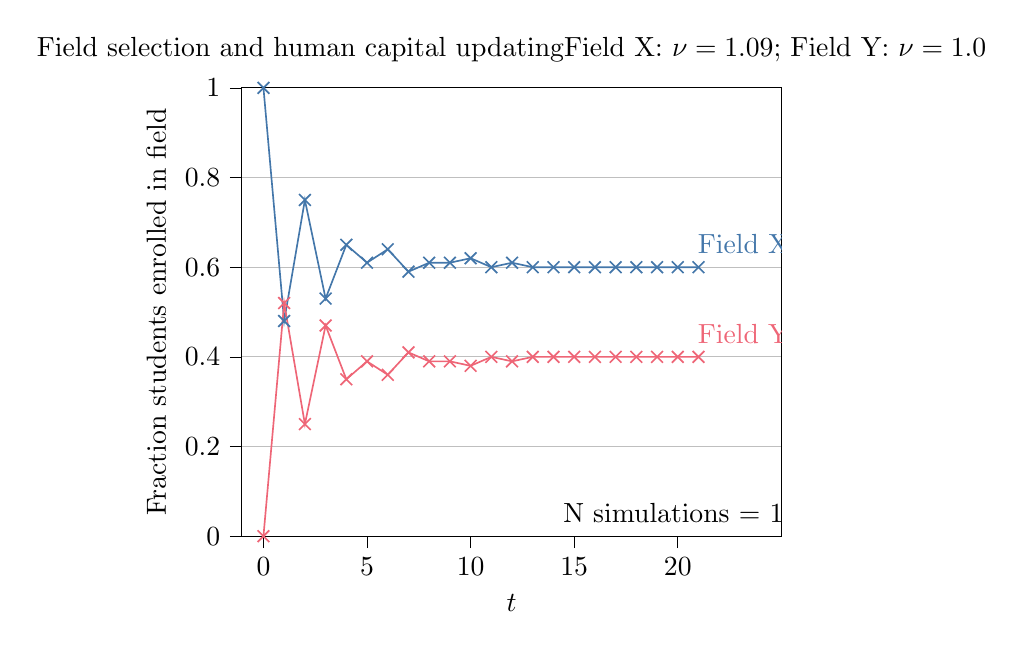
\begin{tikzpicture}

\definecolor{color0}{rgb}{0.266666666666667,0.466666666666667,0.666666666666667}
\definecolor{color1}{rgb}{0.933333333333333,0.4,0.466666666666667}

\begin{axis}[
height=207pt,
tick align=outside,
tick pos=left,
title={Field selection and human capital updating \\ Field X: \(\displaystyle \nu=1.09\); Field Y: \(\displaystyle \nu=1.0\)},
width=240pt,
x grid style={white!69.0196078431373!black},
xlabel={\(\displaystyle t\)},
xmin=-1.05, xmax=25,
xtick style={color=black},
xtick={0,5,10,15,20},
xticklabels={\(\displaystyle 0\),\(\displaystyle 5\),\(\displaystyle 10\),\(\displaystyle 15\),\(\displaystyle 20\)},
ylabel={Fraction students enrolled in field},
ymajorgrids,
ymin=0, ymax=1,
ytick style={color=black},
ytick={0,0.2,0.4,0.6,0.8,1},
yticklabels={\(\displaystyle 0\),\(\displaystyle 0.2\),\(\displaystyle 0.4\),\(\displaystyle 0.6\),\(\displaystyle 0.8\),\(\displaystyle 1\)}
]
\addplot [semithick, color0, mark=x, mark size=3, mark options={solid}]
table {%
0 1
1 0.48
2 0.75
3 0.53
4 0.65
5 0.61
6 0.64
7 0.59
8 0.61
9 0.61
10 0.62
11 0.6
12 0.61
13 0.6
14 0.6
15 0.6
16 0.6
17 0.6
18 0.6
19 0.6
20 0.6
21 0.6
};
\addplot [semithick, color1, mark=x, mark size=3, mark options={solid}]
table {%
0 0
1 0.52
2 0.25
3 0.47
4 0.35
5 0.39
6 0.36
7 0.41
8 0.39
9 0.39
10 0.38
11 0.4
12 0.39
13 0.4
14 0.4
15 0.4
16 0.4
17 0.4
18 0.4
19 0.4
20 0.4
21 0.4
};
\draw (axis cs:20.5,0.63) node[
  anchor=base west,
  text=color0,
  rotate=0.0
]{Field X};
\draw (axis cs:20.5,0.43) node[
  anchor=base west,
  text=color1,
  rotate=0.0
]{Field Y};
\draw (axis cs:14,0.03) node[
  anchor=base west,
  text=black,
  rotate=0.0
]{N simulations = 100};
\end{axis}

\end{tikzpicture}

\end{figure}
\hyperlink{app_ability_v_effect}{\beamerbutton{Return: $\alpha_{X0} \nu_X = \alpha_{Y0} \nu_Y$}}
\hyperlink{sim_beliefs}{\beamerbutton{Return: belief simulation}}
\hyperlink{sim_ability}{\beamerbutton{Return: ability simulation}}

\end{frame}
